\documentclass[11pt,a4paper]{article}
\usepackage{estilosexercicios}

% ---------------------------------------------------
\title{Álgebra Linear}
\author{MAT5730}
\date{2 semestre de 2019}

\begin{document}
\maketitle
\tableofcontents
\newpage
\begin{comment}

\begin{center}
\large\textbf{\textcolor{Floresta}{Lista 1}}\\
\end{center}

\end{comment}

\section{\textcolor{Floresta}{Lista 0}}

\exercicio{1} Seja
\[
\mathbb{Q}(\sqrt{2}) = \{ a + b \sqrt{2} \in \mathbb{R} : a,b \in \mathbb{Q} \}.
\]
\dividiritens{
\task[\pers{a}] Prove que $\mathbb{Q}(\sqrt{2})$ é um corpo.
\task[\pers{b}] Prove que $\mathbb{Q}(\sqrt{2})$ é um $\mathbb{Q}$-espaço vetorial e exiba uma base desse espaço vetorial sobre $\mathbb{Q}.$
\task[\pers{c}] Mostre que se $L$ e $K$ são corpos tais que $K \subset L,$ então $L$ é um $K$-espaço vetorial.
}
\exercicio{2} Seja $V$ um $K$-espaço vetorial e seja $\{u, v, w\} \subset V$ um conjunto linearmente independente.
Determine condições sobre $K$ para que o conjunto $\{u + v, u + w, v + w\}$ também seja linearmente independente.

\exercicio{3} Seja \(S\) um subconjunto de um espaço vetorial \(V\)
sobre um corpo \(K\). Recorde que o subespaço de \(V\) gerado por \(S\)
é definido por
\[\langle S\rangle\coloneqq\{\lambda_1v_1+\ldots+\lambda_nv_n\,\colon
  n\in\Naturals, \lambda_i\in K, v_i\in S\},\]
isto é, \(\langle S\rangle\) é o conjunto de todas as
combinações lineares de vetores em \(S\).

\dividiritens{
    \task[\pers{a}] Mostre que \(\langle S\rangle\) é um subespaço de \(V\).
   \task[\pers{b}] Seja \(W\) a interseção de todos os subespaços de \(V\) que
   contém \(S\). Mostre que \(W=\langle S\rangle\).
}

\solucao{
  \dividiritens{
    \task[\pers{a}]
     Primeiramente note que para qualquer conjunto \(S^\prime\subseteq S\) finito e \(\alpha\colon S^\prime\to\{0\}\) temos que
\(\sum_{x\in S^\prime}\alpha_x x=0\) e logo \(0\in\langle S\rangle\). Além disso, se \(\lambda\in K\)
e \(x\in\langle S\rangle\) temos que \(x=\sum_{x\in S^\prime}\alpha_xx\) para \(S^\prime\subseteq S\) finito e \(\alpha\colon B^\prime\to\Reals\). Então
\[\lambda x =\sum_{x\in S^\prime}(\lambda\alpha_x)x\in \langle S\rangle.\]

Por fim,  sejam \(x,y\in \langle S\rangle\). Então \(x=\sum_{I_x}\alpha_v v\)
e \(y=\sum_{I_y}\beta_v v\) para conjuntos \(I_x, I_y\) finitos e funções
\(\alpha\colon I_x\to\Reals\) e \(\beta\colon I_y\to\Reals\). Defina a função
\(\bar{\alpha}\colon I_x\cup I_y\to\Reals\) dada por \[\bar{\alpha}_v\coloneqq\begin{cases}\alpha_v\,\text{ se } v\in I_x;\\
0, \text{ caso contrário.}\end{cases}\] Similarmente, considere a função \(\bar{\beta}\colon I_x\cup I_y\to \Reals\) dada por \[\bar{\beta}_v\coloneqq\begin{cases}\beta_v\,\text{ se } v\in I_y;\\
0, \text{ caso contrário.}\end{cases}\]Então temos que 
\[x+y=\sum_{v\in I_x}\alpha_v v +\sum_{v\in I_y}\beta_v v=\sum_{v\in I_x\cup I_y}(\bar{\alpha}_v + \bar{\beta}_v) v.\] 
Como \(I_x\cup I_y\) é finito e \(\bar{\alpha}_v+\bar{\beta}_v\in\Reals\) para cada \(v\in I_x\cup I_y\) segue que \(x+y\in \langle S\rangle\).
Concluímos assim que \(0\in\langle S\rangle\), que \(\lambda s\in\langle S\rangle\) para cada \(\lambda\in K\) e cada \(s\in \langle S\rangle\) e que \(x+y\in\langle S\rangle\) sempre que \(x,y\in \langle S\rangle\).
Isto é, \(\langle S\rangle\) é um subespaço. 

     \task[\pers{b}] Considere o seguinte conjunto \[W\coloneqq\bigcap\{U\subseteq V\,\colon U \text{ é subespaço e } S\subseteq U\}.\]
Seja \(U\) um subespaço de \(V\) que contém \(S\). Pela definição de subespaço, obtemos que \(U\) contém todas as combinações lineares de elementos de \(S\). Logo, \(\langle S\rangle\subseteq U\). Concluímos assim que \(\langle S\rangle\) está contido em cada subespaço de \(V\) que contém \(S\) e portanto \(\langle S\rangle\subseteq W\).

 Por outro lado, se \(s\in W\) então \(s\) pertence a cada subespaço de \(V\) que contém \(S\). Pelo item a, temos que
\(\langle S\rangle\) é um subespaço de \(V\) e claramente contém \(S\). Portanto \(s\in\langle S\rangle\).

}}

\exercicio{4} Mostre que um subconjunto $B$ de um espaço vetorial é linearmente independente se, e somente se, todo subconjunto finito de $B$ é linearmente independente.
 

\exercicio{5} Sejam \(W_1\) e \(W_2\) subespaços de um espaço vetorial \(V\).
\dividiritens{ \task[\pers{a}] Dê um exemplo mostrando que \(W_1\cup W_2\) pode
  não ser um subespaço de \(V\).
  \task[\pers{b}] Prove que \(W_1\cup W_2\) é um subespaço se, e somente se
  \(W_1\subseteq W_2\) ou \(W_2\subseteq W_1\).
 \task[\pers{c}] Mostre que \(W_1+W_2\) é o subespaço gerado por \(W_1\cup W_2\).}

\solucao{
  \dividiritens{
    \task[\pers{a}]  Por exemplo, se \(V=\mathbb{R}^2\), \(W_1=\langle(1,0)\rangle\) e 
 \(W_2=\langle(0,1)\rangle\) então \(W_1\cup W_2 \) não é um 
 subespaço de \(V\).
    \task[\pers{b}] Primeiro, suponha sem perda de generalidade que
    \(W_1\subseteq W_2\). Neste caso, temos que \mbox{\(W_1\cup W_2=W_2\),} que é um
    subespaço por hipótese. A outra implicação é a contrapositiva da Proposição
    \ref{unotsubsp} das notas de aula. 
    \task[\pers{c}]  Primeiramente vamos mostrar que \(W_1+W_2\subseteq\langle W_1\cup W_2\rangle\). Se \(w_1+w_2\in W_1+W_2\), então claramente
  \[w_1+w_2=1w_1+1w_2 \text{ com } w_1\in W_1\text{ e }w_2\in W_2.\] 
  Por outro lado,
  seja \(w\in\langle W_1\cup W_2\rangle\). Então podemos escrever \[w=\sum_{v\in I_1\cup I_2}\alpha_vv=\sum_{v\in I_1}\alpha_vv+\sum_{v\in I_2}\alpha_vv,\]
  onde \(I_1\subseteq W_1\) e \(I_2\subseteq W_2\), e \(\alpha\colon I_1\cup I_2\to\mathbb{R}\).  Como \(W_1\) e \(W_2\) são subespaços temos que \(\sum_{v\in I_1}\alpha_v v\in W_1\)
  e \(\sum_{v\in I_2}\alpha_vv\in W_2\) e portanto \(w\in W_1 + W_2\).

}}

\exercicio{6} Considere o $\mathbb{R}$-espaço vetorial $\mathcal{M}_2(\mathbb{R})$ das matrizes de $2 \times 2$ sobre $\mathbb{R}$ e os seguintes subconjuntos de $\mathcal{M}_2(\mathbb{R}):$
\[
W_1 = \left\{ \begin{bmatrix} x & -x \\ y & z \end{bmatrix} : x,y,z \in \mathbb{R} \right\} \quad \mbox{e} \quad W_2 = \left\{ \begin{bmatrix} a & b \\ -a & c \end{bmatrix} : a,b,c \in \mathbb{R} \right\}
\]
\dividiritens{
\task[\pers{a}] Mostre que $W_1$ e $W_2$ são subespaços de $\mathcal{M}_2(\mathbb{R}).$
\task[\pers{b}] Encontre as dimensões de $W_1, W_2, W_1 + W_2$ e $W_1 \cap W_2.$
}

\exercicio{7} Seja \(\mathcal{F}=\{S_i\,\colon i \in I\}\) uma
família não vazia de subespaços distintos de um \(K\)-espaço vetorial \(V\).
Mostre que são equivalentes:
\dividiritens{ \task[\pers{i}]
  Para cada \(i\in I\), temos que \(S_i\cap \Big(\sum\limits_{i\neq j} S_j\Big)=\{0\}\).
  \task[\pers{ii}]
  O vetor nulo não pode ser escrito como uma soma
  de vetores não nulos, cada um pertencendo a um subespaço distinto
  de \(\mathcal{F}\).
  \task[\pers{iii}]
  Todo vetor não nulo de \(\sum_{i\in I}S_i\) tem,
  a menos da ordem, uma decomposição única como soma de vetores não nulos
  \(v=s_1+\ldots +s_n\), com os vetores \(s_1,\ldots , s_n\)
  pertencendo a subespaços distintos de \(\mathcal{F}\).
}
\textbf{Observação:} Segue deste exercício que \(V=\sum\limits_{i\in I}S_i\) é uma
soma direta se, e somente se, uma das condições (i)-(iii) é satisfeita.

\solucao{
  \dividiritens{\task[\pers{a}] \textbf{(i)$\implies$(ii)}: Assuma que existe uma família de elementos
              não nulos \(v_i\in S_i\) tais que \mbox{\(\sum\limits_{i\in I}v_i=0\).} Seja
              \(i_0\in I\) e note que \(v_{i_0}=-\sum\limits_{i\in I\setminus\{i_0\}}v_i\). Como \(S_i\) é um
              subespaço para cada \(i\in I\) concluímos que
              \(v_{i_0}\in\sum\limits_{i\in I\setminus\{i_0\}}S_i\). Como temos que
              \(v_{i_0}\in S_{i_0}\) por construção, concluímos que \(0\neq
              v_{i_0}\in S_{i_0}\cap \Big(\sum\limits_{i\neq i_0}S_i\Big)\) e portanto  a afirmação (i) é falsa.
            \task[\pers{b}] \textbf{(ii) $\implies$ (i)}: Assuma que existe
            \(i_0\in I\) tal que existe
            \(0\neq v_{i_0}\in S_{i_0}\cap\Big(\sum\limits_{i\neq  i_0}S_i\Big).\)
            Neste caso, temos que existe uma família \(\{-v_i\}_{i\in
              I\setminus\{i_0\}}\) com \(v_i\in S_i\) para cada \(i\in
            I\setminus\{i_0\}\) e \(\sum\limits_{i\in I\setminus\{i_0\}}v_i=v_{i_0}\). Dessa forma, temos que a família \(\{v_{i_0}\}\cup\{v_i\}_{i\in
              I\setminus\{i_0\}}\) é uma família não nula com \(v_i\in S_i\)
            para cada \(i\in I\) e \(\sum\limits_{i\in I}v_i=0\). Isto é, a afirmação
            (ii) é falsa.
              \task[\pers{c}]\textbf{(iii) $\implies$ (i)}: Seja \(0\not=s\in\sum\limits_{i\in I}S_i\) e seja
            \(\{s_i\}_{i\in I}\) a única decomposição
            de \(S\). Assuma que existe
            \(0\not =v\in S_{i_0}\cap(\sum\limits_{j\in I\setminus\{i_0\}}S_j)\) para
            algum \(i_0\in I\).
            Neste caso segue que
    \[s=\sum\limits_{i\in I}s_i=(s_{i_0}+v)+\sum\limits_{j\in I\setminus\{i_0\}}s_i -v.\]
    Isto é, \(s\) tem duas decomposições, o que
    é uma contradição.
           \task[\pers{d}]\textbf{(i) $\implies$ (iii)}: Seja \(0\neq
           s\in\sum\limits_{i\in I}S_i\) e assuma que existem duas famílias
           \(\{s_i\}_{i\in I}\) e \(\{v_i\}_{i\in I}\) distintas tais
           que \[\sum\limits_{i\in I} s_i=\sum\limits_{i\in I}v_i=s.\].
           Seja \(i_0\in I\) tal que \(s_{i_0}\neq
           v_{i_0}\). Então \begin{align*}0\not=v_{i_0}-s_{i_0}&=
      \sum\limits_{i\in I\setminus\{i_0\}}s_i-\sum\limits_{i\in I\setminus\{i_0\}}v_i
                              \\&=\sum\limits_{i\in I\setminus\{i_0\}}s_i-v_i.
                            \end{align*}
Assim concluímos que \(0\neq v_{i_0}-s_{i_0}\in S_{i_0}\cap                                                             \Big(\sum\limits_{i\neq
                                                               i_0} S_i\Big)\).
                                                             Isto é, a afirmação (i) é falsa.
          
                                                             \task[\pers{e}]\textbf{(ii) $\implies$ (iii)}: Seja
                                                      \(0\neq s\in V\) e
          assuma que existem duas famílias distintas \(\{v_i\}_{i\in I}\) e
          \(\{s_i\}_{i\in I}\) tais que \[\sum\limits_{i\in I} v_i=\sum\limits_{i\in
              I}s_i=s.\] Neste caso, obtemos que \begin{align*}
                                                   0=s-s&=\sum\limits_{i\in I}s_i-\sum\limits_{i\in I}v_i\\&=\sum\limits_{i \in I}s_i-v_i.
                                                 \end{align*}
                                                 Assim escrevemos o vetor nulo
                                                 como uma soma não nula de
                                                 vetores, cada um pertencendo a
                                                 um subespaço \(S_i\). Isso
                                                 implica que a afirmação (ii) é falsa.
                                                 \task[\pers{f}]\textbf{(iii)$\implies$ (ii)}:
                       Seja \(0\neq v\in V\), seja \(\{v_i\}_{i\in I}\) a única
                       família tal que \(v_i\in S_i\) para cada \(i\in I\)e
                       \(\sum\limits_{i\in I}v_i=v\). Assuma que existe uma
           família \(\{s_i\}_{i\in I}\) não nula de vetores onde \(s_i\in S_i\)
           para cada \(i\in I\) e \(\sum\limits_{i\in I}s_i=0\). Então temos
           que \[v=v+0=\sum\limits_{i\in I}v_i+s_i=\sum\limits_{i\in I}v_i-s_i=v-0=v,\]
           o que nos da uma contradição.
          
         }}

\exercicio{8} Seja  \(V\) um \(K\)-espaço vetorial e seja \(S\) um subconjunto
linearmente independente de \(V\). Mostre que, se \(v\in V\) não for combinação
linear dos elementos de \(S\), então \(S\cup\{v\}\) é linearmente independente.

\solucao{Assuma que \(v\) é combinação linear dos elementos de \(S\). Neste caso
existe \(S^\prime\subseteq S\) finito e uma função \(\alpha\colon S^\prime\to\Reals\) tal que 
\(\sum\limits_{s\in S^\prime}\alpha_s s=v\). Defina \(\bar{\alpha}\colon S^\prime\cup\{v\}\to\Reals\) tal que
\(\bar{\alpha}_s=\alpha_s\) para cada \(s\in S^\prime\) e \(\bar{\alpha}_v=-1\). Então segue que \(\sum\limits_{s\in S^\prime\cup\{v\}}\bar{\alpha}_ss=0.\) Isto é, \(S\cup\{v\}\) é Linearmente dependente.
}

\exercicio{9} Seja \(V\) um \(K\)-espaço vetorial de dimensão finita e sejam
\(U\) e \(W\) subespaços de \(V\) tais que \(V=U+W\). Mostre que \(V=U\oplus
W\), se e somente se, \(\dim (V)=\dim (U)+\dim (W).\)
\solucao{ Utilizando o fato de
  que \[\text{dim}(V)=\text{dim}(W)+\text{dim}(U)-\text{dim}(U\cap W)\]
  e o Exercício 7,
  vemos que as seguintes afirmações são equivalentes:
  \begin{enumerate}
  \item \(V=U\oplus W\);
  \item \(\dim(V)=\dim(U)+\dim(W)\);
  \item \(V=U+W\) e \(\dim(U\cap W)=0\);
  \end{enumerate}
}
\exercicio{10} Seja \(V\) um \(K\)-espaço vetorial e seja \(W\) um subespaço de
\(V\). Mostre que \(W\) possui complemento em \(V\), isto é, que existe um
subespaço \(U\) de \(V\) tal que \(V=U\oplus W\).

\solucao{  Seja \(B_1\) uma base de \(W\). Como \(B_1\) é L.I temos pelo Teorema 1
  das notas de aula que existe uma base \(B\) de \(V\) tal que \(B_1\subseteq B\). Considere
  o conjunto \(B_2\coloneqq B\setminus B_1\) e o subespaço \(U\coloneqq\langle B_2\rangle\). Pelo exercício 3 temos
  que \(U\) é um subespaço e ainda temos do exercício 5 que \mbox{\(V= W+U\)}.
  Resta mostrar que \(U\cap W=\{0\}\). Assuma que existe \(0\not= v\in U|cap
  W\). Neste caso temos que existem conjuntos finitos \(B_1^\prime\subseteq
  B_1\) e \(B_2^\prime\) e funções \(\alpha\colon B_1^\prime\to\Reals\) e
  \(\beta\colon B_2\prime\to\Reals\) tais que
  \[v=\sum\limits_{b\in B_1^\prime}\alpha_bb=\sum\limits_{b\in B_2^\prime}\beta_bb.\]
  Seja \(i_0\in B_1^\prime\) tal que \(\alpha_{i_0}\neq 0 \), então
  \[b_{i_0}=\frac{1}{\alpha_{i_0}}\Big(\sum_{b\in B_2^\prime}\beta_bw-\sum_{i\in
      B_1^\prime\setminus\{i_0\}}\Big),\]
que, pelo exercício 8 implica que \(B_1\cup B_2\) não é L.I. Contradição.
}

\exercicio{11} Seja $V \neq \{0\}$ um espaço vetorial sobre um corpo infinito $K.$ Mostre que $V$ não é uma união de um número finito de subespaços próprios. E se $K$ for finito?\\
\textbf{Sugestão:} Suponha que $V = W_1 \cup W_2 \cup \ldots \cup W_n$ e que $W_1 \nsubseteq W_2 \cup \ldots \cup W_n.$ Sejam $w \in W_1 \setminus(W2 \cup \ldots \cup W_n)$ e $v \notin W_1.$ Seja $A = \{aw + v : a \in K\}$ e mostre que cada $W_i$ contém no máximo um elemento de $A.$)



\exercicio{12} (Lei modular) Seja \(V\) um espaço vetorial. Sejam \(S,U,T\) subespaços de
\(V\). Mostre que se \(U\subseteq S\), então:
\[S\cap(T+U)=(S\cap T)+(S\cap U).\]
\solucao{
  Primeiro, note que como \(U\subseteq S\) temos que \(S\cap U=U\) e portanto é
  suficiente mostrar que \[S\cap(T+U)=(S\cap T)+ U.\]
  Como \( U\subseteq U+T\) e \(U\subseteq S\) temos que
  \begin{equation}\label{0.12.1}U\subseteq (U+T)\cap S.\end{equation} Além disso, como \(T\subseteq U+T\)
  temos que \begin{equation}\label{0.12.2}T\cap S\subseteq (U+T)\cap
    S.\end{equation}
  Assim, juntando as Equações \ref{0.12.1} e \ref{0.12.2} obtemos que \(U+(T\cap
  S)\subseteq (U+T)\cap S.\) Por outro lado, considere \(y\in (U+T)\cap S\).
  Isto é, \(y=u+t=s\) para alguns \(u\in U\), \(t\in T\), e \(s\in S\). Como
  \(U\subseteq S\) e \(S\) é subespaço, obtemos que \(t=s-u\in S\) e concluímos
  que \(t\in T\cap S\). Dessa forma segue que \(y=u+t\in U+(T\cap S).\)  
}

\exercicio{13} Para quais espaços vetoriais \(V\) a lei distributiva
\[S\cap(T+U)=(S\cap T)+(S\cap U)\]
é verdadeira para todos os subespaços \(S,T,U\) de \(V\)?
\solucao{
Vamos iniciar notando que se \(\dim (V)\leq 1\) o resultado vale trivialmente.
Se \(\dim (V)\geq 2\), tomamos dois vetores \(v_t\) e \(v_u\) linearmente
independentes e consideramos \(T\coloneqq\langle v_t\rangle\),
\(U\coloneqq\langle v_u\rangle\) e \(S\coloneqq\langle v_u+v_t\rangle\). Dessa
forma temos \(S\subseteq U+T\) e portanto \(S\cap (U+T)=S\), mas por outro lado
\((S\cap T)=(S\cap U)= 0.\)
}

\exercicio{14} Sejam \(U\) e \(V\) \(K\)-espaços vetoriais e seja \(T\colon U\to
V\) uma transformação linear.
\dividiritens{
    \task[\pers{a}] Prove que \(T\) é injetora se, e somente se, \(T\) leva todo
    subconjunto linearmente independente de \(U\) em um conjunto linearmente
    independente de \(V\).
   \task[\pers{b}] Prove que se o subconjunto \(\{T(u_1),\ldots , T(u_n)\}\) de \(V\) for
   linearmente independente, então \(\{u_1,\ldots , u_n\}\) é um subconjunto
   linearmente independente de \(U\).
}
   
\solucao{}

\exercicio{15} Sejam $U$ e $V$ $K$-espaços vetoriais de dimensão finita tais que $\dim U = \dim V$ e seja $T \colon U \to V$ uma transformação linear. Mostre que as seguintes afirmações são equivalentes:

\dividiritens{
\task[\pers{i}] $T$ é um isomorfismo;
\task[\pers{ii}] $T$ é sobrejetora;
\task[\pers{iii}] $T$ é injetora.
}
\solucao{}
\exercicio{16} Sejam $U$ e $V$ $K$-espaços e seja $T \colon U \to V$ um isomorfismo. Mostre que $T^{-1} \colon V \to U$ também é linear e, portanto, é um isomorfismo.
\solucao{}
\exercicio{17} Seja $V$ um $K$-espaço vetorial e seja $T$ um operador linear de $V$ tal que $T^2 = T$ (um operador
com essa propriedade é chamado de \emph{projeção}). Mostre que \[V = \Ker T \oplus \mbox{Im} T\]
\solucao{}
\exercicio{18} Seja $V$ um $K$-espaço vetorial de dimensão finita e seja $T$ um operador linear de $V.$ Mostre que as seguintes afirmações são equivalentes:
\dividiritens{
\task[\pers{i}] $\Ker^2 T = \Ker T;$
\task[\pers{ii}] $\mbox{Im}^2 T = \mbox{Im } T;$
\task[\pers{iii}] $V = \Ker T \oplus \mbox{Im } T.$
}

\solucao{%https://www.ime.usp.br/~leila/2011p1.pdf 
}
\exercicio{19} Seja $V$ um $K$-espaço vetorial de dimensão finita e seja $T \colon V \to V$ uma transformação linear tal que $\mbox{posto} T^2 = \mbox{posto} T.$ Prove que $\Ker T \cap \mbox{Im } T = \{0\}.$
\solucao{}
\exercicio{20} Seja $V$ um $K$-espaço vetorial e sejam $S, T \in \mathcal{L}(V).$ Mostre que
\[
T(\Ker(S \circ T)) = \Ker S \cap \mbox{Im } T
\]
\solucao{}
\exercicio{21} Sejam $V$ e $W$ dois espaços vetoriais sobre o corpo $K$ e sejam $S$ e $T$ duas transformações lineares de $V$ em $W,$ ambas de posto finito. Mostre que $S + T$ tem posto finito e que
\[
\abs{\mbox{posto } S - \mbox{posto } T} \le \mbox{posto }(T + S) \le \mbox{posto } S + \mbox{posto } T
\]
\solucao{}
\exercicio{22} Seja $V$ um espaço vetorial de dimensão $n$ sobre o corpo $K$ e sejam $S$ e $T$ dois operadores
lineares em $V$. Suponha que $S \circ T = 0$ e que $S + T$ é sobrejetora. Mostre que 
\[
\mbox{posto } T + \mbox{posto } S = n
\]
\solucao{}
\exercicio{23} Seja $T$ um operador linear de posto $1$ em um espaço vetorial $V.$ Mostre que existe um único
escalar $\alpha$ tal que $T^2 = \alpha T.$ Prove que se $\alpha \neq 1,$ então $I- T$ é inversível.

\solucao{}
\exercicio{24}  Seja $V$ um espaço vetorial sobre um corpo $K$ de característica diferente de $2$ e seja $T$ um
operador linear em $V$ tal que $T^2 = I.$ Prove que ou $T = I,$ ou $T = -I,$ ou existe uma base $B$ base de $V$ tal que
\[
[T]_{B} = \begin{bmatrix}
1 & 0 \\
0 & -1
\end{bmatrix}
\]
Dê um exemplo para mostrar que a hipótese $\mbox{char}(K) \neq 2$ é necessária.
\solucao{}
\exercicio{25} Seja $V$ um espaço vetorial sobre um corpo $K$ de característica diferente de $2$ e seja $T$ um
operador linear em $V$ tal que $T^2 = I.$ Sejam 
\[W = \{v \in V : T(v) = v\} \quad \mbox{e} \quad U = \{v \in V : T(v) = -v\}.\] Prove que 
\[V = W \oplus U.\] 
\solucao{}
\exercicio{26} Seja $V$ um $K$-espaço vetorial de dimensão $n$ e seja $T$ um operador linear em $V$ tal que $T^n = 0$ e $T^{n-1} \neq 0$. Seja $v \in V$ tal que $T^{n-1}(v) \neq 0.$ Prove que o conjunto
\[\mathcal{B} = \{v, T(v), T^2(v), \ldots, T^{n-1}(v) \}\]
é uma base de $V$. Qual é a matriz $[T]_{\mathcal{B}}?$ 

\solucao{}
\exercicio{27} Sejam $f_1, \ldots , f_m \in (K^n)^{*}.$ Considere a função $T \colon K^n \to K^m$ definida por
\[T(v) = (f_1(v), f_2(v), \ldots,f_m(v)). \]
Mostre que $T \in \mathcal{L}(K^n, K^m)$ e que toda transformação linear em $\mathcal{L}(K^n, K^m)$ tem essa forma, para alguma escolha adequada de $f_1, \ldots , f_m \in (K^n)^{*}.$
\solucao{}
\exercicio{28} Seja $V$ um $K$-espaço vetorial e seja \[B = \{v_i
: i \in I\}\] uma base de $V$. Para cada $i \in I,$ seja $f_i \in V^*$ tal que $f_i(v_j) = \delta_{ij},$ para todo $j \in I.$
\dividiritens{
\task[\pers{a}] Mostre que \[C = {f_i
: i \in I} \] é linearmente independente.
\task[\pers{b}]) Mostre que $C$ é uma base de $V^{*}$ se, e somente se, $I$ é finito. 
}
\solucao{}
\exercicio{29} Seja $V$ um $K$-espaço vetorial e seja $f \in V^{*}$ um funcional linear não nulo. Mostre que existe $v \in V$ tal que $V = \Ker f \oplus \prin{v}.$
\solucao{}
\exercicio{30} Seja $V$ um $K$-espaço vetorial e sejam $f,g \in V^{*}.$ Mostre que se $\Ker f = \Ker g,$ então existe $\lambda \in K,$ tal que $f(v) = \lambda g(v),$ para todo $v \in V.$ 
\solucao{}
\exercicio{31} Seja $K$ um corpo infinito e seja $V$ um espaço vetorial de dimensão finita sobre $K.$ Sejam $v_1, v_2, \ldots v_m$ vetores não nulos de $V.$ Prove que existe um funcional linear $f \in V^{*}$ tal que $f(v_i)\neq 0$ para todo $i = 1, 2, \ldots ,m.$ 
\solucao{}
\exercicio{32} Seja $V$ um $K$-espaço vetorial. Mostre que $v \in V$ é o vetor nulo se, e somente se $f(v) = 0,$ para todo $f \in V^{*}.$
\solucao{}
\exercicio{33} Seja $\tr: \mathcal{M}_n(K) \to K$ a função traço definida por
\[
\tr(A) = \displaystyle\sum\limits_{i=1}^n a_{ii},
\]
para $A = [a_{ij}]_{1\le,j\le n}$.
\dividiritens{
\task[\pers{a}] Mostre que $\tr$ é linear e que \[\tr(AB) = \tr(BA),\] para quaisquer $A, B \in \mathcal{M}_n(K).$
\task[\pers{b}] Mostre que matrizes semelhantes possuem o mesmo traço.
\task[\pers{c}] Prove que o traço em $\mathcal{M}_n(K)$ é único no seguinte sentido: Se $f \in (\mathcal{M}_n(K))^{*}$ é tal que $f(AB) = f(BA),$ para quaisquer matrizes $A, B \in \mathcal{M}_n(K),$ então existe $\alpha \in K$ tal que $f = \alpha \tr.$ Se, além disso, $f(I_n) = n$ e a característica de $K$ é zero, então $f = \tr.$
}
\solucao{}
\exercicio{34} Sejam $U$ e $W$ subespaços de um $K$-espaço vetorial $V$. Prove que $U = W$ se, e somente se, $U^{0} = W^{0}.$

\solucao{}
\exercicio{35} Sejam $U$ e $W$ subespaços de um $K$-espaço de dimensão finita $V$. Prove que: 
\dividiritens{
\task[\pers{a}] $(U + W)^0= U^0 \cap W^0;$
\task[\pers{b}] $(U \cap W)^{0} = U^0 + W^0.$
}
A condição sobre a dimensão de $V$ é necessária?
\solucao{}
\exercicio{36} Seja $V$ um $K$-espaço de dimensão finita. Mostre que a função $T \mapsto T^t$ é um isomosfismo de $\mathcal{L}(V)$ em $\mathcal{L}(V^{*}).$
\solucao{}
\exercicio{37} Seja $V = \mathcal{P}_n(\mathbb{R}).$ Determine $T^t$ uma base de $\Ker T^t$ para os seguintes operadores lineares $T$ de $V:$
\dividiritens{
\task[\pers{a}] $T$ é o operador derivação em $V;$
\task[\pers{b}] $T(p(t)) = p(t+1),$ para todo $p \in V.$
}
\solucao{}
\newpage
\section{\textcolor{Floresta}{Lista 1}}


\exercicio{1} Sejam $V$ um $K$-espaço vetorial e $W$ um subespaço de $V.$ Seja $S = \{v_i\}_{i\in I} \subset V$ tal que $\overline{S} = \{v_i + W\}_{i\in I}$ é linearmente independente no espaço quociente $V/W.$ Mostre que se $A$ é um conjunto linearmente independente de $W$ então $S \cup A$ é um conjunto linearmente independente de $V.$
\solucao{Se $\overline{S} = \{\overline{v_i} = v_i + W\}_{i\in I}$ é LI em $V/W,$ isso significa que, para todo $M \subseteq I$ finito, temos que, para $\alpha_m \in K,$ com $m \in M,$ ocorre
\[
\sum\limits_{m \in M} \alpha_m \overline{v_m} = 0 \Rightarrow \alpha_m = 0 \ \forall \ m \in M
\]

Seja $A = \{ w_j \}_{j \in J}.$ Por hipótese, sabemos também que $A$ é um conjunto linearmente independente, ou seja, para todo $N \subseteq I$ finito, temos que, para $\alpha_n \in K,$ com $n \in N,$ ocorre
\[
\sum\limits_{n \in N} \alpha_n w_n = 0 \Rightarrow \alpha_n = 0, \ \forall \ n \in N
\]

Para mostrar que $S \cup A = \{v_i\}_{i\in I} \cup \{ w_j \}_{j \in J} = \{ u_p \}_{p \in I \cup J}$ é um conjunto linearmente independente de $V,$ precisamos mostrar que, para todo $L \subset I \cup J$ finito, temos que, para $\alpha_\ell \in K,$ com $\ell \in L,$ ocorre
\[
\sum\limits_{\ell \in L} \alpha_\ell u_\ell = 0 \Rightarrow \alpha_\ell = 0, \ \forall \ \ell \in L
\]

Para fazer isso, precisamos antes verificar se existem vetores que são comuns aos dois subconjuntos, ou seja, calcular $S \cap A.$ Observe que
\[
s \in S \Rightarrow \overline{s} \in \overline{S} 
\]
Como $\overline{S}$ é um conjunto linearmente independente em $W,$ temos que $\overline{s} \neq \overline{0}.$ Portanto, segue que $s - 0 \notin W \Rightarrow s \notin W.$
Mas como $A \subseteq W,$ então isso quer dizer que $s \notin A.$ Portanto, concluímos que $S \cap A = \emptyset.$ Isso quer dizer que todos os $v_i$'s são diferentes dos $w_j$'s, e mais ainda, que $I \cup J$ é uma união disjunta.

Logo, considerando novamente $S \cup A = \{v_i\}_{i\in I} \cup \{ w_j \}_{j \in J}$, para todo $L \subseteq I \cup J$ finito, existem $I^{\prime} \subseteq I$ e $J^{\prime} \subseteq J$ tais que $I^{\prime} \cup J^{\prime} = L.$ Desse modo, temos que
\[
\sum\limits_{\ell \in L} \alpha_\ell u_\ell = 0 \Rightarrow
\]
\[
\sum\limits_{i \in I^{\prime}} \alpha_i v_i + \sum\limits_{j \in J^{\prime}} \alpha_j w_j = 0 \quad \mbox{em } V \Rightarrow 
\]\[
\overline{\sum\limits_{i \in I^{\prime}} \alpha_i v_i + \sum\limits_{j \in J^{\prime}} \alpha_j w_j} = \overline{0} \quad \mbox{em } V/W \Rightarrow 
\]
\[
\sum\limits_{i \in I^{\prime}} \alpha_i \overline{v_i} + \underbrace{\sum\limits_{j \in J^{\prime}} \alpha_j \overline{w_j}}_{= 0, \mbox{ pois } w_j \in W}  = \overline{0} \Rightarrow \sum\limits_{i \in I^{\prime}} \alpha_i \overline{v_i} = \overline{0} \Rightarrow \alpha_i = 0 \ \forall \ i \in I^{\prime},
\]
pois $\{v_i\}_{i \in I^{\prime}} \subseteq \overline{S}$ é um conjunto linearmente independente.

Assim, usando agora o fato de que $\{w_j\}_{j \in J^{\prime}} \subseteq A$ é um conjunto linearmente independente em $W,$ temos que
\[
\textcolor{red}{\sum\limits_{i \in I^{\prime}} \alpha_i v_i} + \sum\limits_{j \in J^{\prime}} \alpha_j w_j = 0 \Rightarrow \textcolor{red}{0} + \sum\limits_{j \in J^{\prime}} \alpha_j w_j = 0 \Rightarrow  \sum\limits_{j \in J^{\prime}} \alpha_j w_j = 0 \Rightarrow \alpha_j = 0 \ \forall \ j \in  J^{\prime}
\]
Concluímos portanto que
\[
\sum\limits_{\ell \in L} \alpha_\ell u_\ell = 0 \Rightarrow \alpha_\ell = 0 \ \forall \ \ell \in L
\]
Daí, $S \cup A$ é um conjunto linearmente independente em $V.$
}

\exercicio{2} Sejam $V$ um $K$-espaço vetorial e $W$ um subespaço de $V.$ Seja $S = \{v_i\}_{i \in I} \subset V$ tal que $S = \{v_i + W\}_{i \in I}$ gera o espaço quociente $V/W.$ Mostre que se $A$ é um conjunto gerador de
$W$ então $S \cup A$ é um conjunto gerador de $V$.
\solucao{
Se $\overline{S} = \{\overline{v_i} = v_i + W\}_{i\in I}$ gera em $V/W,$ isso significa que, para todo $\overline{v} \in V/W,$ existem $M \subseteq I$ finito e $\alpha_m \in K,$ com $m \in M,$ tais que
\[
\overline{v} = \sum\limits_{m \in M} \alpha_m \overline{v_m}
\]

Seja $A = \{ w_j \}_{j \in J}.$ Por hipótese, sabemos também que $A$ gera $W$, ou seja, para todo $w \in W,$ existem $N \subseteq J$ finito e $\alpha_n \in K,$ com $n \in N,$ tais que
\[
w = \sum\limits_{n \in N} \alpha_n w_n
\]

Precisamos mostrar que $S \cup A = \{v_i\}_{i\in I} \cup \{ w_j \}_{j \in J} = \{ u_p \}_{p \in I \cup J}$ é um conjunto gerador para $V,$ ou seja, que para todo $v \in V,$ existem $L \subset I \cup J$ finito e $\alpha_\ell \in K,$ com $\ell \in L,$ tais que
\[
v = \sum\limits_{\ell \in L} \alpha_\ell u_\ell
\]
Note que, como $\overline{S}$ é um conjunto gerador de $V/W,$ temos como já foi explicitado acima que, para $\overline{v} \in V/W,$
\[
\overline{v} = \sum\limits_{m \in M} \alpha_m \overline{v_m} \Rightarrow \overline{v} - \sum\limits_{m \in M} \alpha_m \overline{v_m} = \overline{0} \Rightarrow v - \sum\limits_{m \in M} \alpha_m v_m \in W
\]
Como $A = \{ w_j \}_{j \in J}$ é conjunto gerador para $W,$ temos que existem $N \subseteq J$ finito e $\alpha_n \in K,$ com $n \in N,$ tais que
\[
v - \sum\limits_{m \in M} \alpha_m v_m  = \sum\limits_{n \in N} \alpha_n w_n
\]
Assim, tomando $L = N \cup M$:
\[
v  = \sum\limits_{m \in M} \alpha_m v_m + \sum\limits_{n \in N} \alpha_n w_n \Rightarrow v = \sum\limits_{\ell \in L} \alpha_\ell u_\ell
\]
Portanto, $S \cup A$ é um conjunto gerador para $V.$
}

\exercicio{3} Seja $V$ um $K$-espaço vetorial e sejam $U$ e $W$ subespaços de $V.$ Prove:
\dividiritens{
    \task[\pers{a}] O Segundo Teorema do Isomorfismo:
    \[
    \frac{U + W}{W} \cong \frac{U}{U \cap W}.
    \]
        \task[\pers{b}] O Terceiro Teorema do Isomorfismo: Se $U \subset W,$
        \[
        \frac{V}{W} \cong \frac{V/U}{W/U}
        \]
}

\solucao{
\dividiritens{
    \task[\pers{a}] A intenção será encontrar uma transformação linear adequada para poder aplicar o Primeiro Teorema do Isomorfismo e concluir o resultado desejado. Considere a aplicação
    \[
\fullfunction{T}{U}{\frac{U + W}{W}}{u}{T(u) = \overline{u} = u + W}
    \]
    
    Observe que $T$ é uma transformação linear. De fato, segue trivialmente que:
    \begin{itemize}
        \item[$\clubsuit$] $\forall u, v \in V,$ temos que
        \[
        T(u + v) = \overline{u + v} = (u+v) + W = \textcolor{Green}{u + W} + \textcolor{Blue}{v + W} = \textcolor{Green}{\overline{u}} + \textcolor{Blue}{\overline{v}} = T(u) + T(v)  \]
        
        \item[$\textcolor{Red}{\varheart}$] $\forall u \in W, \forall \alpha \in K,$ temos que
        \[
        T(\alpha u) = \overline{\alpha u} = \alpha u + W = \alpha(\textcolor{Laranja}{u + W}) = \alpha(\textcolor{Laranja}{\overline{u}}) = \alpha T(u)
        \]
    \end{itemize}
    
    Sendo $T$ uma transformação linear, temos do Primeiro Teorema do Isomorfismo que
    \[
    \frac{V/U}{\Ker T} \cong \mbox{Im } T
    \]
    Calculemos $\Ker T$ e $\mbox{Im } T:$
    \begin{itemize}
        \item[$\spadesuit$] $\mbox{Im } T = \frac{U + W}{W}.$ Mostremos que $T$ é sobrejetora:
        
        Para $a \in \frac{U + W}{W},$ dado por $a = \overline{u + w},$ onde $u \in U$ e $w \in W,$ temos que
        \[
        a = \overline{u+ w} = (u+w) + W = (u+W) + \textcolor{DarkOrchid}{(w+W)} = (u + W) + \textcolor{DarkOrchid}{(0 + W)} = \]\[(u + 0) + W = u + W = \overline{u} = T(u)\]
        
        Logo, para todo $a  \in \frac{U + W}{W},$ existe um $u \in U$ tal que $T(u) = a.$ Logo, $T$ é sobrejetora, e portanto $\mbox{Im } T = \frac{U + W}{W}.$
        \item[$\textcolor{Red}{\vardiamond}$] $\Ker T = U \cap W.$ Claramente, sabemos que, como $\Ker T = \{ u \in U : T(u) = \overline{0} \},$ temos que $\Ker T \subset U.$ Mas também temos que, para $a \in \Ker T,$ segue que $a \in U,$ e
        \[
        T(a) = \overline{0} = 0 + W \Rightarrow a - 0 \in W \Rightarrow a \in W
        \]
        Portanto, segue que $a \in U \cap W.$ Daí, $\Ker T = U \cap W.$
    \end{itemize}
    Finalmente, obtemos do Primeiro Teorema do Isomorfismo que
    \[
    \frac{U}{\textcolor{Mahogany}{\Ker T}} \cong \textcolor{NavyBlue}{\mbox{Im } T} \Rightarrow \frac{U}{\textcolor{Mahogany}{U \cap W}} \cong \textcolor{NavyBlue}{\frac{U + W}{W}}.
    \]
    
    \task[\pers{b}] Utilizando a mesma estratégia do item (a), considere a aplicação
    \[
    \fullfunction{T}{\frac{V}{U}}{\frac{V}{W}}{v + U}{T(v + U) = v + W}
    \]
    }
    Vejamos que $T$ está bem-definida, ou seja, representantes de uma mesma classe de equivalência no domínio correspondem a representantes de uma mesma classe de equivalência na imagem. Temos, para $\overline{v_1} = v_1 + U, \overline{v_2} = v_2 + U \in \frac{V}{U},$ que
    
    \[
    \overline{v_1} = \overline{v_2} \Rightarrow v_1 - v_2 \in U \subset W \Rightarrow v_1 - v_2 \in W \Rightarrow v_1 + W = v_2 + W.
    \]
    
    Note que utilizamos fortemente o fato de que $U \subset W$ para mostrar que $T$ está bem-definida. Além disso, $T$ é uma transformação linear. De fato:
    \begin{itemize}
        \item[$\clubsuit$] $\forall v_1 + U, v_2 + U \in \frac{V}{U},$ temos que
        \[  T((v_1 + U) + (v_2 + U)) = T((v_1 + v_2) + U) = (v_1 + v_2) + W = \]\[\textcolor{Green}{(v_1 + W)} + \textcolor{Blue}{(v_2 + W)} = \textcolor{Green}{T(v_1 + U)} + \textcolor{Blue}{T(v_2 + U)} \]
        
        \item[$\textcolor{Red}{\varheart}$] $\forall v + U \in \frac{V}{U}, \forall \alpha \in K,$ temos que
        \[
        T(\alpha v + U) =  \alpha v + W  = \alpha \textcolor{Laranja}{(v + W)} =   \alpha \textcolor{Laranja}{T(v + U)}
        \]
    \end{itemize}
    
    Sendo $T$ uma transformação linear, temos do Primeiro Teorema do Isomorfismo que
    \[
    \frac{U}{\Ker T} \cong \mbox{Im } T
    \]
    Calculemos $\Ker T$ e $\mbox{Im } T:$
    \begin{itemize}
        \item[$\spadesuit$] $\mbox{Im } T = \frac{V}{W}.$ Claramente $T$ é sobrejetora:
        
        Para $v + W \in \frac{V}{W},$ temos que
        \[
        v + W = T(v + U)\]
        
        Logo, para todo $v + W  \in \frac{V}{W},$ existe um $v + U \in \frac{V}{U}$ tal que $T(v + U) = v + W.$ Logo, $T$ é sobrejetora, e portanto $\mbox{Im } T = \frac{V}{W}.$
        \item[$\textcolor{Red}{\vardiamond}$] $\Ker T = \frac{W}{U}.$ Observe que
        \[
        v + U \in \Ker T \Leftrightarrow T(v + U) = v + W = 0 + W \Leftrightarrow v \in W \Leftrightarrow v + U \in \frac{W}{U}.
        \]
        Logo, $\Ker T = \frac{W}{U}.$
    \end{itemize}
    Finalmente, obtemos do Primeiro Teorema do Isomorfismo que
    \[
    \frac{V/U}{\textcolor{Mahogany}{\Ker T}} \cong \textcolor{NavyBlue}{\mbox{Im } T} \Rightarrow \frac{V/U}{\textcolor{Mahogany}{W/U}} \cong \textcolor{NavyBlue}{\frac{V}{W}}.
    \]
    
    
    



}

\exercicio{4} Seja $V$ um $K$-espaço vetorial e sejam $U$ e $W$ subespaços de $V$ tais que12 $\dim (V/U) = m$ e $\dim (V/W) = n.$ Prove que $\dim (V/(U \cap W)) \le m + n.$

\solucao{Das informações fornecidas no enunciado, sabemos que:
\[
\dim (V/U) = m \Rightarrow \dim(V) - \dim(U) = m
\]
\[
\dim (V/W) = n \Rightarrow \dim(V) - \dim(W) = n
\]
Somando essas duas equações obtemos:
\[
2\dim(V) - (m+n) = \dim(U) + \dim(W).
\]
Sabemos também que, se $U$ e $W$ são subespaços de $V,$ então
\[
\dim(U) + \dim(W) = \dim(U \cap W) + \dim(U + W)
\]

Estamos interessados em encontrar $\dim(V/(U \cap W)) = \dim(V) - \dim(U \cap W).$
Observe que, como $U$ e $W$ são subespaços de $V,$ então $\dim(V) \ge \dim(U + W).$ Desse modo,
\[
\dim(U) + \dim(W)  = \dim(U \cap W) + \textcolor{Blue}{\dim(U + W)} \le \dim(U \cap W) + \textcolor{Blue}{\dim(V)} 
\]
Então:
\[
\textcolor{Verde}{\dim(U) + \dim(W)} \le \dim(U \cap W) +\dim(V) \Rightarrow \textcolor{Verde}{2\dim(V) - (m+n) } \le \dim(U \cap W) +\dim(V) \Rightarrow \]\[-(m+n) \le \dim(U \cap W) - \dim(V) \Rightarrow \dim(V) -  \dim(U \cap W) \le m+n
\]
Portanto, concluímos que
\[
\dim(V/(U \cap W)) = dim(V) -  \dim(U \cap W) \le m+n \Rightarrow \boxed{\dim(V/(U \cap W))  \le m + n}
\]
}

\exercicio{5} Mostre que
\dividiritens{
    \task[\pers{a}] $W \oplus U= W^{\prime} \oplus U^{\prime} \ \mbox{e} \ W \cong W^{\prime} \nrightarrow U \cong U^{\prime}.$
   \task[\pers{b}] $V \cong V^{\prime}, V = W \oplus U \ \mbox{e} \ V^{\prime} = W \oplus U^{\prime} \nrightarrow U \cong U^{\prime}.$
}


\solucao{
\dividiritens{
    \task[\pers{a}] Considere $K$ um corpo, e seja
    \[
    V = \bigoplus_{i=1}^\infty Ke_i
    \]
Considere 
\[
    W = \bigoplus_{i=1}^\infty Ke_{2i}
\]
Observe que $W \subseteq V,$ e além disso, $W \cong V.$ Temos também que 
\[
V = W \oplus \left(  \bigoplus_{i=1}^\infty Ke_{2i+1} \right)
\]
}
Portanto, tomando
\[
W = \bigoplus_{i=1}^\infty Ke_{2i}, \ U = \bigoplus_{i=1}^\infty Ke_{2i+1}, \ W^{\prime} = V, \ \mbox{e} \ U^{\prime} = \{ 0 \},
\]
temos que
\[
\left( \bigoplus_{i=1}^\infty Ke_{2i} \right) \oplus \left(  \bigoplus_{i=1}^\infty Ke_{2i+1} \right) \cong V \cong V \oplus \{ 0 \} \Rightarrow W \oplus U= W^{\prime} \oplus U^{\prime}
\]
e
\[
\bigoplus_{i=1}^\infty Ke_{2i} \cong \bigoplus_{i=1}^\infty Ke_i \Rightarrow W \cong W \prime,
\]
mas
\[
\bigoplus_{i=1}^\infty Ke_{2i+1} \ncong \{ 0 \} \Rightarrow U \ncong U^{\prime}
\]

\dividiritens{
        \task[\pers{b}] Considere $K^\mathbb{N} = \{ (a_0, a_1, a_2, \ldots ) | a_i \in K \},$ e sejam:
        \[
        V_i = \{ (0, a_1, 0, a_3, \ldots ) | a_{2i+1} \in K \} \quad \mbox{e} \quad V_p = \{ (a_0,0, a_2, 0, \ldots ) | a_{2i} \in K \}.
        \]
        Tome $V = K^\mathbb{N},$ $V^{\prime} = V_i,$ $U = V_p$ e $U^{\prime} = \{ 0 \}.$ 
        Temos então que $V \cong V^{\prime},$ pois $K^\mathbb{N} \cong V_i,$ e também \[V = V_i \oplus V_p = W \oplus U \quad \mbox{e} \quad V^{\prime} = V_i \oplus \{ 0 \} = W \oplus U^{\prime},\] mas \[V_p \ncong \{ 0 \} \Rightarrow U \ncong U^{\prime}.\] Portanto, temos que
        \[
        \left.\begin{array}{l}
        V \cong V^{\prime} \\ V = W \oplus U \\ V^{\prime} = W \oplus U^{\prime}\\
        \end{array} \right \} \nRightarrow U \cong U^{\prime}
        \]
    }
\textbf{Observação:} Cabe salientar que ambos os itens dessa questão são válidos quando $V$ é um espaço vetorial de dimensão finita.
}

\exercicio{6} Seja $V$ um espaço vetorial e seja $W$ um subespaço de $V.$ Suponha que $V = V_1 \oplus \ldots \oplus V_n$ e $S = S_1 \oplus \ldots \oplus S_n,$ com $S_i \subseteq V_i$ subespaços de $V$ para todo $i = 1, \ldots, n.$ Mostre que
\[
\frac{V}{S} \cong \frac{V_1}{S_1} \oplus \ldots \oplus \frac{V_n}{S_n}.
\]
\solucao{
Sabemos que, se $V$ é soma direta de $ V_1 \oplus \ldots \oplus V_n,$ então todo $v \in V$ pode ser escrito como soma de elementos de $V_i$ \textbf{de maneira única}. Podemos escrever então
\[v = \sum\limits_{i = 1}^n v_i\]

O mesmo se aplica a $S.$ Dito isso, considere a aplicação
\[
\fullfunction{T}{V = \bigoplus\limits_{i=1}^n V_i = V_1 \oplus \ldots \oplus V_n}{\bigoplus\limits_{i=1}^n  \frac{V_i}{S_i} =  \frac{V_1}{S_1} \oplus \ldots \oplus \frac{V_n}{S_n} }{v = \sum\limits_{i = 1}^n v_i}{T(v) = \sum\limits_{i = 1}^n (v_i + S_i)}
\]
Verifiquemos que $T$ é uma transformação linear:
\begin{itemize}
    \item Para todo $u, v \in V,$ podemos escrever de maneira única $u = \sum\limits_{i =1}^n u_i$ e $v = \sum\limits_{i =1}^n v_i$. Portanto, temos
    \[T(u) + T(v) = T\left(\sum\limits_{i=1}^n u_i \right) + T\left(\sum\limits_{i=1}^n v_i \right) = \sum\limits_{i=1}^n (u_i + S_i) +  \sum\limits_{i=1}^n (v_i + S_i) =  \]\[\sum\limits_{i=1}^n ((u_i + S_i) + (v_i + S_i)) = T(u + v) \Rightarrow T(u) + T(v) = T(u+v).\]
    \item Para todo $v \in V,$ podemos escrever de maneira única $v = \sum\limits_{i =1}^n v_i;$ assim, para $\alpha \in K:$
    \[
    T(\alpha v) = T\left(\alpha \sum\limits_{i=1}^n v_i \right) =   T\left( \sum\limits_{i=1}^n \alpha v_i \right) = T\left( \sum\limits_{i=1}^n \alpha v_i \right) = \sum\limits_{i=1}^n (\alpha v_i + S_i) = \]\[ \sum\limits_{i=1}^n \alpha (v_i + S_i)  = \alpha \sum\limits_{i=1}^n (v_i + S_i) = \alpha T(v) \Rightarrow T(\alpha v) = \alpha T(v) 
    \]
\end{itemize}
Logo, $T$ é uma transformação linear. Vamos utilizar o Primeiro Teorema do Isomorfismo em $T.$ Para isso, calculemos o núcleo e a imagem de $T:$
\begin{itemize}
    \item $\mbox{Im} (T):$ Dado $u \in \bigoplus\limits_{i=1}^n  \frac{V_i}{S_i},$ temos que esse elemento pode ser escrito de maneira única como 
    \[
    u = \sum\limits_{i = 1}^n (u_i + S_i),
    \]
    onde $u_i \in V_i.$ Então temos que
        \[
    u = \sum\limits_{i = 1}^n (u_i + S_i) = T\left(  \sum\limits_{i = 1}^n u_i \right).
    \]
    Logo, $T$ é sobrejetora, e 
    \[
    \mbox{Im}(T) = \bigoplus\limits_{i=1}^n  \frac{V_i}{S_i} =  \frac{V_1}{S_1} \oplus \ldots \oplus \frac{V_n}{S_n} 
    \]
    \item $\mbox{Ker} (T):$ Considere $v \in \mbox{Ker}(T).$ Então, tomando $v = \sum\limits_{i=1}^n v_i,$ temos que
    \[
 v \in \mbox{Ker}(T) \Rightarrow T(v) = 0 \Rightarrow T\left(\sum\limits_{i=1}^n v_i \right) = 0 \Rightarrow \sum\limits_{i=1}^n (v_i + S_i) = 0 \Rightarrow \]\[v_i + S_i = 0, \ \forall i \in  \{1, \ldots, n\} \Rightarrow v_i \in S_i , \ \forall i \in  \{1, \ldots, n\} \Rightarrow v \in S
    \]
    Assim, $\mbox{Ker}(T) \subseteq S.$
    Agora, tome $s \in S.$ Então, como $S = \bigoplus\limits_{i=1}^n S_i,$ então podemos escrever $s$ de maneira única como
    \[
    s = \sum\limits_{i = 1}^n s_i,
    \]
    onde $s_i \in S_i,$ para $i = 1, \dots, n.$
    Desse modo,
    \[
    T(s) = T\left(  \sum\limits_{i = 1}^n s_i \right) = \sum\limits_{i = 1}^n (s_i + S_i) = \underbrace{\sum\limits_{i = 1}^n (0 + S_i)}_{\mbox{pois } s_i \in S_i \ \forall i} = 0.
    \]
    Assim, $S \subseteq \mbox{Ker}(T).$
    Concluímos que $\mbox{Ker}(T) = S.$
\end{itemize}

Pelo Primeiro Teorema do Isomorfismo, temos que
\[
    \frac{V}{\textcolor{Blue}{\mbox{Ker}(T)}} \cong \textcolor{Verde}{\mbox{Im}(T)} \Rightarrow  \frac{V}{\textcolor{Blue}{S}} \cong \textcolor{Verde}{ \bigoplus\limits_{i=1}^n  \frac{V_i}{S_i}} 
\]
Então:
\[
\frac{V}{S} \cong \frac{V_1}{S_1} \oplus \ldots \oplus \frac{V_n}{S_n},
\]
como queríamos.
}

\exercicio{7} Seja $V$ um $K$-espaço vetorial e seja $W$ um subespaço de $V.$ Seja $T \in \mathcal{L}(V)$ e defina $\overline{T} \colon V/W \to V/W$ por
\[
\overline{T}(v+ W) = T(v) + W, \mbox{ para todo } v + W \in V/W.
\]
\dividiritens{
    \task[\pers{a}]  Determine uma condição necessária e suficiente sobre $W$ para que $\overline{T}$ esteja bem definida.
   \task[\pers{b}]  Se $\overline{T}$ estiver bem definida, mostre que ela é linear e determine seu núcleo e sua imagem.
}
\solucao{
\dividiritens{
    \task[\pers{a}] Seja
    \[   \fullfunction{\pi}{V}{V/W}{v}{\pi(v) = v +W}\]
    A projeção canônica de $V$ em $V/W.$ Então, podemos considerar o seguinte diagrama:
    

\begin{center}

\tikzset{every picture/.style={line width=0.75pt}} %set default line width to 0.75pt        

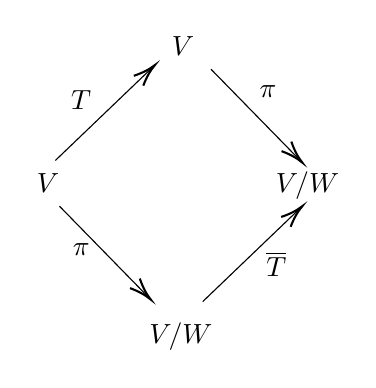
\begin{tikzpicture}[x=0.75pt,y=0.75pt,yscale=-1,xscale=1]
%uncomment if require: \path (0,300); %set diagram left start at 0, and has height of 300

%Straight Lines [id:da34889049551168805] 
\draw    (62.5,94) -- (109.06,49.38) ;
\draw [shift={(110.5,48)}, rotate = 496.22] [color={rgb, 255:red, 0; green, 0; blue, 0 }  ][line width=0.75]    (10.93,-3.29) .. controls (6.95,-1.4) and (3.31,-0.3) .. (0,0) .. controls (3.31,0.3) and (6.95,1.4) .. (10.93,3.29)   ;

%Straight Lines [id:da3558445685185325] 
\draw    (133.5,162) -- (180.06,117.38) ;
\draw [shift={(181.5,116)}, rotate = 496.22] [color={rgb, 255:red, 0; green, 0; blue, 0 }  ][line width=0.75]    (10.93,-3.29) .. controls (6.95,-1.4) and (3.31,-0.3) .. (0,0) .. controls (3.31,0.3) and (6.95,1.4) .. (10.93,3.29)   ;

%Straight Lines [id:da04986735852274893] 
\draw    (137.5,50) -- (180.1,93.57) ;
\draw [shift={(181.5,95)}, rotate = 225.64] [color={rgb, 255:red, 0; green, 0; blue, 0 }  ][line width=0.75]    (10.93,-3.29) .. controls (6.95,-1.4) and (3.31,-0.3) .. (0,0) .. controls (3.31,0.3) and (6.95,1.4) .. (10.93,3.29)   ;

%Straight Lines [id:da9800428074288963] 
\draw    (64.5,116) -- (107.1,159.57) ;
\draw [shift={(108.5,161)}, rotate = 225.64] [color={rgb, 255:red, 0; green, 0; blue, 0 }  ][line width=0.75]    (10.93,-3.29) .. controls (6.95,-1.4) and (3.31,-0.3) .. (0,0) .. controls (3.31,0.3) and (6.95,1.4) .. (10.93,3.29)   ;


% Text Node
\draw (124,39) node  [align=left] {$V$};
% Text Node
\draw (59,105) node  [align=left] {$V$};
% Text Node
\draw (184,106) node  [align=left] {$V/W$};
% Text Node
\draw (123,179) node  [align=left] {$V/W$};
% Text Node
\draw (75,65) node  [align=left] {$T$};
% Text Node
\draw (165,61) node  [align=left] {$\displaystyle \pi $};
% Text Node
\draw (75,137) node  [align=left] {$\displaystyle \pi $};
% Text Node
\draw (169,144) node  [align=left] {$\displaystyle \overline{T}$};


\end{tikzpicture}

\end{center}
Note que $\pi \circ T = \overline{T} \circ \pi.$ Daí, $\overline{T}$ estará bem-definida se $\Ker(\pi) \subseteq \Ker(\pi \circ T).$ Claramente, temos que $\Ker(\pi) = W.$ Vamos calcular $ \Ker(\pi \circ T).$ Temos que
\[v \in \Ker(\pi \circ T) \Leftrightarrow  \pi ( T(v)) = \overline{0} \Leftrightarrow T(v) \in W \Leftrightarrow v \in T^{-1}\]

Logo, temos que 
\[\textcolor{Blue}{\Ker(\pi)} \subseteq \textcolor{Verde}{\Ker(\pi \circ T)} \Rightarrow \textcolor{Blue}{W} \subseteq \textcolor{Verde}{T^{-1}(W)} \Rightarrow T[W] \subseteq W.\]
Portanto, uma condição necessária e suficiente para $\overline{T}$ estar bem definida é que para todo $v \in W,$ tenhamos $T(v) \in W,$ ou seja, $T(W) \subseteq W.$

Em outras palavras, $\overline{T}$ está bem definida se $W$ for um subespaço $T$-invariante de $V.$
    \task[\pers{b}] Verifiquemos que $\overline{T}$ é uma transformação linear. Temos:
    \begin{itemize}
        \item[$\textcolor{red}{\vardiamond}$] Para todos $u + W, v + W \in V/W,$ lembrando que $T$ é linear, temos que
     \[        \overline{T}((u+W) + (v + W)) = \overline{T}((u+v)+ W) = \textcolor{RawSienna}{T(u+v)} + W = \textcolor{RawSienna}{T(u)+T(v)}+ W = \]\[\textcolor{red}{(T(u) + W)} + \textcolor{Laranja}{(T(v) + W)} = \textcolor{red}{\overline{T}(u+W)} + \textcolor{Laranja}{\overline{T}(v+W)}      \]
        Logo, $\overline{T}(\overline{u}+\overline{v}) = \overline{T}(\overline{u})+ \overline{T}(\overline{v}).$
        \end{itemize}
        }
        \newpage
        \begin{itemize}
       \item[$\clubsuit$] Para todo $v + W \in V/W,$ e para todo $\alpha \in K,$ temos que
       \[         \overline{T}(\alpha(v+W)) = \overline{T}( (\alpha v)+W) = \textcolor{RawSienna}{T(\alpha v)} + W = \textcolor{RawSienna}{\alpha T(v)} + W =  \]\[ \alpha \textcolor{Laranja}{(T(v) +W)} = \alpha \textcolor{Laranja}{\overline{T}(v + W)}       \]
        Portanto, $\overline{T}(\alpha \overline{v}) = \alpha \overline{T}(\overline{v}).$
    \end{itemize}
    
    Vamos encontrar o núcleo e a imagem de $\overline{T}.$
    \begin{itemize}
        \item[$\textcolor{red}{\varheart}$] Sendo $\overline{v} = v + W \in V/W,$ observe que
        \[
        \overline{T}(\overline{v}) = 0 \Rightarrow \overline{T(v)}=0 \Rightarrow T(v) \in W \Rightarrow v \in T^{-1}(W).
        \]
        Portanto, temos que
        \[
        \Ker(\overline{T}) = \{ \overline{v} | v \in T^{-1}(W) \}.
        \]
        
     \item[$\spadesuit$] Vamos verificar que $\overline{T}$ é sobrejetora. Sabemos que $\pi$ é sobrejetora. Então, temos que
     \[
     \begin{array}{lcr}
     \mbox{Im}(\overline{T}) &=&    \mbox{Im}(\overline{T} \circ \pi) \\
     &=&    \mbox{Im}(\pi \circ T) \\
     &=&    \{ \pi(T(v)) : v \in V \} \\
     &=&    \{ \overline{T(v)} : v \in V \} \\
     \end{array}
     \]
     Portanto, temos que
     \[
     \mbox{Im}(\overline{T}) = V/W.
     \]
    \end{itemize}

    }

\exercicio{8} Seja $T \in \mathcal{L}(\mathbb{R}^3)$ o operador linear definido por $T(x, y, z) = (x, x, x).$ Seja $T \colon \mathbb{R}^3/W \to \mathbb{R}^3/W$
tal que $\overline{T}((x, y, z) + W) = T(x, y, z) + W,$ em que $W = \mbox{Ker } T.$ Descreva $\overline{T}.$

\solucao{Veja que $\overline{T}$ está bem definida, pois $W = \Ker (T)$ é um subespaço $T$-invariante de $V.$ Vamos encontrar o núcleo e a imagem de $\overline{T}.$
\begin{itemize}
    \item Do exercício anterior, temos que
            \[
        \Ker(\overline{T}) = \{ \overline{v} | v \in T^{-1}(W) \}.
        \]
        Em particular,
                    \[  \Ker(\overline{T}) = \{ \overline{v} | v \in T^{-1}(\Ker T) \} = \{ \overline{v} | v \in T^{-1}(\Ker T) \} \]
        Então segue que
        \[
        v \in T^{-1}(\Ker T)  \Rightarrow T(v) \in \Ker(T) \Leftrightarrow T(T(v)) = 0.
        \]
        Mas $T(T(v)) = T(v).$ De fato, para $v = (x,y,z) \in \mathbb{R}^3,$ temos 
        \[
        T(T(v)) = T(\textcolor{Cyan}{T(x,y,z)}) = T(\textcolor{Cyan}{x,x,x}) = (x,x,x) = T(x,y,z) = T(v)
        \]
        Daí, como para $v \in T^{-1}(\Ker T),$ temos $T(T(v)) = 0,$
        \[
        \textcolor{Emerald}{T(T(v))} = 0 \Rightarrow  \textcolor{Emerald}{T(v)} = 0
        \]
        
    Além disso, se $v \in \Ker (T) = W,$ temos $\overline{v} = 0.$
    
    Portanto, concluímos que $\Ker (\overline{T}) = \{ 0 \},$ ou seja, $\overline{T}$ é injetora.
    \item Do exercício anterior, temos
       \[
     \mbox{Im}(\overline{T}) = V/W.
     \]
     Logo, $\mbox{Im}(\overline{T}) = \mathbb{R}^3/\Ker T.$
     Podemos também descrever $\mbox{Im}(\overline{T})$ da seguinte maneira:
     \[
     \begin{array}{rcl}
     \mbox{Im}(\overline{T}) &=& \{ \overline{T(v)} : v \in V \} \\
     &=& \{ T(v) + \Ker T | v = (x,y,z) \in \mathbb{R}^3 \} \\
     &=& \{ (x,x,x) +  \textcolor{PineGreen}{\Ker T} | x \in \mathbb{R} \} \\
     &=& \{ (x, x,x) + \textcolor{PineGreen}{(0,y,z)} | x,y,z \in \mathbb{R} \} \\
        &=& \{ (x, x+y,x+z) | x,y,z \in \mathbb{R} \} \\  
     \end{array}
     \]
\end{itemize}

}

\exercicio{9} Sejam $V$ e $U$ $K$-espaços vetoriais. Seja $W$ um subespaço de $V$ e $\pi \colon V \to V/W$ a projeção canônica. Mostre que a função $\mathcal{L}(V/W, U) \to \mathcal{L}(V, U),$ dada por $T \to T \circ \pi,$ é injetora.

\solucao{
Temos a função\[\fullfunction{\varphi}{\mathcal{L}(V/W, U)}{ \mathcal{L}(V, U)}{T}{T \circ \pi}\]Para mostrar que $\varphi$ é injetora, precisamos verificar que, para $T \in \mathcal{L}(V/W, U),$ se $\varphi(T) = 0,$ então $T \cong 0.$ Note que
\[
\varphi(T) = 0 \Rightarrow T \circ \pi = 0 \Rightarrow T(\pi(v)) = 0.
\]
Vamos mostrar que $T(u) = 0 \ \forall u \in V/W.$ Sabemos que $\pi$ é sobrejetora. Assim, dado $u \in V/W,$ existe $v \in V$ tal que $u = \pi(v).$ Logo,
\[
T(\textcolor{Green}{u}) = T(\textcolor{Green}{ \pi(v)}) = (T \circ \pi)(v) = 0.
\]
Portanto, $T(u) = 0 \ \forall u \in V/W.$ Daí, $\Ker (\varphi) = \{ 0 \}.$

Concluímos que $\varphi$ é injetora.

%Verifiquemos primeiramente que $\varphi$ é uma transformação linear:\[(\varphi(S) - \varphi(T))(v) = \varphi(S - T)(v) = ((S - T) \circ \pi)(v) = (S-T)(\pi(v)) = S\]
}

\exercicio{10} Seja $V$ um $K$-espaço vetorial e seja $W$ um subespaço de $V.$ Mostre que $(V/W)^{*} \cong W^{0}$ e que $V^{*}/W^{0} \cong W^{*}.$

\solucao{Mostremos que $(V/W)^{*} \cong W^{0}.$ Para isso, a ideia será utilizar a aplicação canônica de $V$ em $V/W$ e sua transposta, e depois aplicar o Primeiro Teorema do Isomorfismo para obter o resultado desejado. Comecemos considerando a aplicação canônica
\[
\fullfunction{T}{V}{V/W}{v}{T(v) = v + W}
\]
Veja que $T$ é sobrejetora (isto é, $\mbox{Im } T = V/W$), e $\mbox{Ker } T = W.$ Consideremos a aplicação transposta
\[\fullfunction{T^t}{(V/W)^{*}}{V^{*}}{f}{T^t(f) = f \circ T}
\]
Das propriedades da transformação transposta, sabemos que
\[
\mbox{Ker } T^t = (\textcolor{Laranja}{\mbox{Im } T})^{0} = (\textcolor{Laranja}{V/W})^{0} = \{0\}
\]
\[
\mbox{Im } T^t = (\textcolor{Rosadif}{\mbox{Ker } T})^{0} = \textcolor{Rosadif}{W}^{0}
\]
Pelo Primeiro Teorema do Isomorfismo, temos que
\[
\frac{(V/W)^{*}}{\textcolor{Laranja}{\mbox{Ker } T^t}} \cong \textcolor{Rosadif}{\mbox{Im } T^t } \Rightarrow \frac{(V/W)^{*}}{\textcolor{Laranja}{\{ 0 \}}} \cong \textcolor{Rosadif}{W^{0}} \Rightarrow \boxed{ (V/W)^{*} \cong W^0}
\]

Mostremos agora que $V^{*}/W^{0} \cong W^{*}.$ Utilizaremos a mesma estratégia, mas considerando agora a inclusão. Tome a inclusão de $W$ em $V,$ isto é:
\[
\fullfunction{\iota}{W}{V}{w}{\iota(w) = w}
\]
Note que $\mbox{Ker }\iota = \{ 0 \}$ e $\mbox{Im } \iota = W.$
Seja
\[
\fullfunction{\iota^t}{V^{*}}{W^{*}}{f}{\iota(f) = f \circ \iota}
\]
a transposta de $\iota.$ Observe que
\[
\mbox{Ker } \iota^t = (\textcolor{Laranja}{\mbox{Im } \iota})^{0} = \textcolor{Laranja}{W}^{0} 
\]
\[
\mbox{Im } \iota^t = (\textcolor{Rosadif}{\mbox{Ker } \iota})^{0} = \textcolor{Rosadif}{\{0\}}^{0} = W^{*}\]
Pelo Primeiro Teorema do Isomorfismo,
\[\frac{V^{*}}{\textcolor{Laranja}{\mbox{Ker } \iota^t}} \cong \textcolor{Rosadif}{\mbox{Im }\iota^t }\Rightarrow \frac{V^{*}}{\textcolor{Laranja}{W^{0}}} \cong \textcolor{Rosadif}{W^{*}} \Rightarrow \boxed{ V^{*}/W^0 \cong W^{*}}\]
}

\exercicio{11} Sejam $A,B,C \in \mathcal{M}_n(K).$ Prove que
\[
\det \left[ \begin{array}{cc} 0 & C \\ A & B \end{array} \right] = (-1)^n \det(A) \det(C).
\]
\solucao{Considere
\[
\fullfunction{F_1}{\mathcal{M}_n(K)}{K}{X}{F_1(X) = \det \begin{bmatrix} 0 & X \\ A & B \end{bmatrix}}
\]
Observe que $F_1$ é $n$-linear e alternada nas linhas de $X.$ Logo, existe um $\lambda_1 \in K$ tal que
\[
F_1(X) = \lambda_1 \det(X).
\]
Em particular,
\[
\lambda_1 = \lambda_1 \cdot \textcolor{RubineRed}{1} = \lambda_1 \textcolor{RubineRed}{\det (I_n)} = F_1(I_n) = \det \begin{bmatrix} 0 & I_n \\ A & B \end{bmatrix} \Rightarrow \boxed{\lambda_1 =\det \begin{bmatrix} 0 & I_n \\ A & B \end{bmatrix}}
\]
Considere agora
\[
\fullfunction{F_2}{\mathcal{M}_n(K)}{K}{Y}{F_2(Y) = \det \begin{bmatrix} 0 & I_n \\ Y & B \end{bmatrix}}
\]
Temos que $F_2$ é $n$-linear e alternada nas colunas de $Y.$ Logo, existe um $\lambda_2 \in K$ tal que 
\[
F_2(Y) = \lambda_2 \det(Y).
\]
Além disso,
\[
\lambda_2 = \lambda_2 \cdot \textcolor{RubineRed}{1} = \lambda_2 \textcolor{RubineRed}{\det (I_n)} = F_2(I_n) = \det \begin{bmatrix} 0 & I_n \\ I_n & B \end{bmatrix} = (-1)^n \Rightarrow \boxed{\lambda_2 = (-1)^n}
\]

Logo,
\[
\lambda_1 = \det \begin{bmatrix} 0 & I_n \\ A & B \end{bmatrix} = F_2(A) = \textcolor{OliveGreen}{\lambda_2} \det(A) = \textcolor{OliveGreen}{(-1)^n}\det(A)
\]
Consequentemente,
\[
 \det \begin{bmatrix} 0 & C \\ A & B \end{bmatrix} = F_1(C) = \textcolor{RawSienna}{\lambda_1} \det(C) = \textcolor{RawSienna}{(-1)^n \det(A)} \det(C)
\]
Portanto, concluímos que 
\[
\det \left[ \begin{array}{cc} 0 & C \\ A & B \end{array} \right] = (-1)^n \det(A) \det(C).
\]
\textbf{Observação:} Mas porquê $\det \begin{bmatrix} 0 & I_n \\ I_n & B \end{bmatrix} = (-1)^n?$ Vamos explicitar essa matriz:
\[M = \begin{bmatrix} 0 & \textcolor{Green}{I_n} \\ \textcolor{Red}{I_n} & B \end{bmatrix} =
 \left[\begin{array}{ccccc|ccccc} 0 & 0 & 0 & \ldots & 0 & \textcolor{Green}{1} & \textcolor{Green}{0} & \textcolor{Green}{0} & \textcolor{Green}{\ldots} & \textcolor{Green}{0} \\ 
 0 & 0 & 0 & \ldots & 0 & \textcolor{Green}{0} & \textcolor{Green}{1} & \textcolor{Green}{0} & \textcolor{Green}{\ldots} & \textcolor{Green}{0} \\ 
 0 & 0 & 0 & \ldots & 0 & \textcolor{Green}{0} & \textcolor{Green}{0} & \textcolor{Green}{1} & \textcolor{Green}{\ldots} & \textcolor{Green}{0} \\
 \vdots & \vdots & \vdots & \ddots & \vdots & \textcolor{Green}{\vdots}& \textcolor{Green}{\vdots} & \textcolor{Green}{\vdots} & \textcolor{Green}{\ddots} & \textcolor{Green}{\vdots} \\ 
  0 & 0 & 0 & \ldots & 0 & \textcolor{Green}{0} & \textcolor{Green}{0} & \textcolor{Green}{0} & \textcolor{Green}{\ldots} & \textcolor{Green}{1} \\ \hline
  
  \textcolor{Red}{1} & \textcolor{Red}{0} & \textcolor{Red}{0} & \textcolor{Red}{\ldots} & \textcolor{Red}{0} & b_{11} & b_{12} & b_{13} & \ldots & b_{1n} \\
\textcolor{Red}{0} & \textcolor{Red}{1} & \textcolor{Red}{0} & \textcolor{Red}{\ldots} & \textcolor{Red}{0} & b_{21} & b_{22} & b_{23} & \ldots & b_{2n} \\ 
\textcolor{Red}{0} & \textcolor{Red}{0} & \textcolor{Red}{1} & \textcolor{Red}{\ldots} & \textcolor{Red}{0} & b_{31} & b_{32} & b_{33} & \ldots & b_{3n} \\ 
\textcolor{Red}{\vdots} &\textcolor{Red}{\vdots} & \textcolor{Red}{\vdots} & \textcolor{Red}{\ddots} & \textcolor{Red}{\vdots} & \vdots & \vdots & \vdots & \ddots & \vdots \\ 
\textcolor{Red}{0} & \textcolor{Red}{0} & \textcolor{Red}{0} & \textcolor{Red}{\ldots} & \textcolor{Red}{1} & b_{n1} & b_{n2} & b_{n3} & \ldots & b_{nn} \\ 
 \end{array}\right]\]
Por definição, temos que \[\det M = \sum\limits_{\sigma \in S_{2n}} \sgn(\sigma) m_{1\sigma(1)} m_{2 \sigma(2)} \ldots m_{2n \sigma(2n)}.\]
Mas observe que $m_{1 \sigma(1)} \neq 0$ apenas quando $\sigma(1) = n + 1.$ Também temos que  $m_{2 \sigma(2)} \neq 0$ apenas quando $\sigma(2) = n + 2.$ Analogamente, concluímos que, para todo $k \le n,$
\[
m_{k \sigma(k)} = \begin{cases}
1, & \mbox{se } \sigma(k) = n + k;\\
0, & \mbox{caso contrário.}
\end{cases},
\]
já que $m_{k \sigma(k)}$ estará na área em \textcolor{Green}{verde} na matriz. Portanto, os somandos serão não nulos somente para as permutações que satisfazem $\sigma(k) = n + k,$ para $k \le n.$ Então, temos  que para $n < \ell \le 2n,$ $\sigma(\ell) = p,$ onde $p \in \{1, 2, \ldots, n \}$
Agora, veja que $m_{\ell \sigma(\ell)}$ se encontrará na área em \textcolor{Red}{vermelho} na matriz, e portanto
\[
m_{\ell \sigma(\ell)} = \begin{cases}
1, & \mbox{se } \sigma(\ell) = \ell - n;\\
0, & \mbox{caso contrário.}
\end{cases}
\]
Logo, a única permutação para a qual $m_{g \sigma(g)} \neq 0 \ \forall g \in \{1, 2, \ldots, 2n \}$ será a permutação
\[
\rho = (1 \ \ n+1) (2 \ \ n+2) \ldots (n \ \ 2n),
\]
que é composta por uma quantidade ímpar de transposições, se $n $ é ímpar, ou por uma quantidade par de transposições, se $n$ é par. Logo, $\sgn(\rho) = (-1)^n.$ Portanto, concluímos que
 \[\det M = \sum\limits_{\sigma \in S_{2n}} \sgn(\sigma) m_{1\sigma(1)} m_{2 \sigma(2)} \ldots m_{2n \sigma(2n)} = \textcolor{Magenta}{\sgn(\rho)} m_{1 \textcolor{Magenta}{\rho(1)}} m_{2 \textcolor{Magenta}{\rho(2)}} \ldots m_{2n \textcolor{Magenta}{\rho(2n)}} =\]\[ \textcolor{Magenta}{(-1)^n} m_{1 \textcolor{Magenta}{(n+1)}} m_{2 \textcolor{Magenta}{(n+2)}} \ldots m_{2n \textcolor{Magenta}{(n)}} = (-1)^n \]
}

\exercicio{12} Calcule o determinante da matriz de Vandermonde, isto é, prove que
\[
\det \left[ \begin{array}{cccc} 1 & 1 & \ldots & 1 \\ c_1 & c_2 & \ldots & c_n \\ \vdots & \vdots & \ddots & \vdots \\ c_1^{n-1} & c_2^{n-1} & \ldots & c_n^{n-1} \end{array} \right] = \prod\limits_{1 \le i < j \le n} (c_j - c_i)
\]
\solucao{
Vamos provar o resultado por indução sobre $n \ge 2.$ Para $n = 2,$ é fácil ver que
\[
\det \left[ \begin{array}{cc} 1 & 1 \\ c_1 & c_2 \end{array} \right] = c_2 - c_1 = \prod\limits_{1 \le i < j \le 2} (c_j - c_i)
\]
Assuma o resultado válido para $n - 1,$ ou seja, 
\[
\det \left[ \begin{array}{cccc} 1 & 1 & \ldots & 1 \\ c_1 & c_2 & \ldots & c_n \\ \vdots & \vdots & \ddots & \vdots \\ c_1^{n-2} & c_2^{n-2} & \ldots & c_n^{n-2} \end{array} \right] = \prod\limits_{1 \le i < j \le n-1} (c_j - c_i) = \prod\limits_{1 \le i < j \le n-1} (c_j - c_i)
\]
Provemos para a matriz $n \times n.$ Utilizando a matriz transposta, vamos aplicar operações nas colunas da matriz de modo a obter zeros na primeira linha. Para isso, vamos multiplicar cada coluna $C_i$ por $-c_1$ e somaremos com a coluna $C_{i+1},$ obtendo
\[\begin{bmatrix} 
\textcolor{Laranja}{1} & \textcolor{Verde}{c_1} & \textcolor{Blue}{c_1^2} & \textcolor{RawSienna}{\dots} & \textcolor{Purple}{c_1^{n-1}}\\
\textcolor{Laranja}{1} & \textcolor{Verde}{c_2} & \textcolor{Blue}{c_2^2} & \textcolor{RawSienna}{\dots}  & \textcolor{Purple}{c_2^{n-1}}\\ 
\textcolor{Laranja}{1} & \textcolor{Verde}{c_3} & \textcolor{Blue}{c_3^2} & \textcolor{RawSienna}{\dots}  &  \textcolor{Purple}{c_3^{n-1}}\\ 
\textcolor{Laranja}{\vdots} & \textcolor{Verde}{\vdots} & \vdots &\textcolor{RawSienna}{\ddots}  &\vdots \\ 
\textcolor{Laranja}{1} & \textcolor{Verde}{c_n} & \textcolor{Blue}{c_n^2} & \textcolor{RawSienna}{\dots}  &  \textcolor{Purple}{c_n^{n-1}}\\ \end{bmatrix} \xrightarrow{C_{i+1} = C_{i+1} - \textcolor{red}{c_1}C_i} \begin{bmatrix} \textcolor{Laranja}{1} & \textcolor{Verde}{c_1} - \textcolor{red}{c_1}\textcolor{Laranja}{1}  & \textcolor{Blue}{c_1^2} - \textcolor{red}{c_1}\textcolor{Verde}{c_1} & \textcolor{RawSienna}{\dots}  & \textcolor{Purple}{c_1^{n-1}} - \textcolor{red}{c_1}\textcolor{RawSienna}{c_1^{n-2}}\\ 
\textcolor{Laranja}{1} & \textcolor{Verde}{c_2}  - \textcolor{red}{c_1}\textcolor{Laranja}{1}  &  \textcolor{Blue}{c_2^2} - \textcolor{red}{c_1}\textcolor{Verde}{c_2}  & \textcolor{RawSienna}{\dots}  & \textcolor{Purple}{c_2^{n-1}} - \textcolor{red}{c_1}\textcolor{RawSienna}{c_2^{n-2}}\\ 
\textcolor{Laranja}{1} &  \textcolor{Verde}{c_3}  - \textcolor{red}{c_1}\textcolor{Laranja}{1} & \textcolor{Blue}{c_3^2} - \textcolor{red}{c_1}\textcolor{Verde}{c_3}  & \textcolor{RawSienna}{\dots}  & \textcolor{Purple}{c_3^{n-1}} - \textcolor{red}{c_1}\textcolor{RawSienna}{c_3^{n-2}}\\
\vdots & \vdots & \vdots & \ddots  &\vdots \\ 
\textcolor{Laranja}{1} &  \textcolor{Verde}{c_n}  - \textcolor{red}{c_1}\textcolor{Laranja}{1}  & \textcolor{Blue}{c_n^2} - \textcolor{red}{c_1}\textcolor{Verde}{c_n} & \textcolor{RawSienna}{\dots}  & \textcolor{Purple}{c_n^{n-1}} - \textcolor{red}{c_1}\textcolor{RawSienna}{c_n^{n-2}}\\ \end{bmatrix}=\]
\[\begin{bmatrix} 1 & 0 & 0 & \dots & 0\\ 1 & c_2-c_1 & c_2(c_2-c_1) & \dots & c_2^{n-2}(c_2-c_1)\\ 1 & c_3-c_1 & c_3(c_3-c_1) & \dots & c_3^{n-2}(c_3-c_1)\\ \vdots & \vdots & \vdots & \ddots &\vdots \\ 1 & c_n-c_1 & c_n(c_n-c_1) & \dots & c_n^{n-2}(c_n-c_1)\\ \end{bmatrix}\]

Utilizando o Teorema de Laplace, temos que
\[
\det \left[\begin{array}{c|cccc} 1 & 0 & 0 & \dots & 0\\ \hline 1 & c_2-c_1 & c_2(c_2-c_1) & \dots & c_2^{n-2}(c_2-c_1)\\ 1 & c_3-c_1 & c_3(c_3-c_1) & \dots & c_3^{n-2}(c_3-c_1)\\ \vdots & \vdots & \vdots & \ddots &\vdots \\ 1 & c_n-c_1 & c_n(c_n-c_1) & \dots & c_n^{n-2}(c_n-c_1)\\ \end{array}\right] =\]\[ \det \left[\begin{array}{cccc}   c_2-c_1 & c_2(c_2-c_1) & \dots & c_2^{n-2}(c_2-c_1)\\  c_3-c_1 & c_3(c_3-c_1) & \dots & c_3^{n-2}(c_3-c_1)\\  \vdots & \vdots & \ddots &\vdots \\ c_n-c_1 & c_n(c_n-c_1) & \dots & c_n^{n-2}(c_n-c_1)\\ \end{array}\right]
\]
Como cada linha está multiplicada por $c_i - c_1,$ por propriedades do determinante, temos que
\[
\det \left[\begin{array}{cccc}   \textcolor{Verde}{c_2-c_1} & c_2\textcolor{Verde}{(c_2-c_1)} & \dots & c_2^{n-2}\textcolor{Verde}{(c_2-c_1)}\\  \textcolor{Blue}{c_3-c_1} & c_3\textcolor{Blue}{(c_3-c_1)} & \dots & c_3^{n-2}\textcolor{Blue}{(c_3-c_1)}\\  \vdots & \vdots & \ddots &\vdots \\ \textcolor{Red}{c_n-c_1} & c_n\textcolor{Red}{(c_n-c_1)} & \dots & c_n^{n-2}\textcolor{Red}{(c_n-c_1)}\\ \end{array}\right] =\]\[
\textcolor{Verde}{(c_2-c_1)}\textcolor{Blue}{(c_3-c_1)} \cdot \ldots \cdot  \textcolor{Red}{(c_n-c_1)}  \det \left[\begin{array}{ccccc}   1& c_2 & c_2^2 & \dots & c_2^{n-2}\\  1 & c_3 & c_3^2 & \dots & c_3^{n-2} \\  1 & c_4 & c_4^2 & \dots & c_4^{n-2}\\  \vdots & \vdots & \ddots &\vdots \\ 1 & c_n & c_n^2 & \dots & c_n^{n-2}\\ \end{array}\right] = \]\[
\prod\limits_{j = 2}^n (c_j - c_1)  \det \left[\begin{array}{ccccc}   1& c_2 & c_2^2 & \dots & c_2^{n-2}\\  1 & c_3 & c_3^2 & \dots & c_3^{n-2} \\  1 & c_4 & c_4^2 & \dots & c_4^{n-2}\\  \vdots & \vdots & \ddots &\vdots \\ 1 & c_n & c_n^2 & \dots & c_n^{n-2}\\ \end{array}\right] 
\]
Como a matriz resultante tem tamanho $n-1 \times n-1,$ da hipótese de indução, vem
\[
 \det \left[\begin{array}{ccccc}   1& c_2 & c_2^2 & \dots & c_2^{n-2}\\  1 & c_3 & c_3^2 & \dots & c_3^{n-2} \\  1 & c_4 & c_4^2 & \dots & c_4^{n-2}\\  \vdots & \vdots & \ddots &\vdots \\ 1 & c_n & c_n^2 & \dots & c_n^{n-2}\\ \end{array}\right] =  \prod\limits_{2 \le i < j \le n} (c_j - c_i).
\]
Daí,
\[
\left(\prod\limits_{j = 2}^n (c_j - c_1) \right) \textcolor{red}{\det \left[\begin{array}{ccccc}   1& c_2 & c_2^2 & \dots & c_2^{n-2}\\  1 & c_3 & c_3^2 & \dots & c_3^{n-2} \\  1 & c_4 & c_4^2 & \dots & c_4^{n-2}\\  \vdots & \vdots & \ddots &\vdots \\ 1 & c_n & c_n^2 & \dots & c_n^{n-2}\\ \end{array}\right]} = \]\[\left(\prod\limits_{j = 2}^n (c_j - c_1) \right) \textcolor{red}{\left(\prod\limits_{2 \le i < j \le n} (c_j - c_i) \right)} = \prod\limits_{1 \le i < j \le n} (c_j - c_i) 
\]
Assim, segue o resultado.
}

\exercicio{13} Mostre que
\[
\det \left[ \begin{array}{cccc} a & -b & -c & -d \\ b & a & -d & c \\ c & d & a & -b \\ d & -c & b & a \end{array} \right] = (a^2 + b^2 + c^2 + d^2)^2
\]
\solucao{ 
Considere
\[
A = \begin{bmatrix} a & -b \\ b & a \end{bmatrix} \quad \mbox{ e } \quad B = \begin{bmatrix} c & d \\ d & -c \end{bmatrix},
\]
e seja
\[
C  = \det \begin{bmatrix} A & -B \\ B & A \end{bmatrix}
\]
Observe que a matriz $CC^t$ é diagonal, já que as colunas são ortogonais. Como $\det(C) = \det(C^t),$ temos que
\[
\det(C^2) = \det(C) \textcolor{Red}{\det(C)} = \det(C) \textcolor{Red}{\det(C^t)} = \det(CC^t)
\]
De fato, temos que
\[
CC^t = \left(\begin{matrix}
a^2+b^2+c^2+d^2 & 0 & 0 & 0 \\
0 & a^2+b^2+c^2+d^2 & 0 & 0 \\
0 & 0 & a^2+b^2+c^2+d^2 & 0 \\
0 & 0 & 0 & a^2+b^2+c^2+d^2
\end{matrix}\right)
\]
Daí, 
\[
\det(CC^t) = (a^2+b^2+c^2+d^2)^4
\]
Portanto, 
\[
(\det(C))^2 = \det(CC^t) = (a^2+b^2+c^2+d^2)^4 \Rightarrow \det(C) = \pm (a^2+b^2+c^2+d^2)^2.
\]
Mas observe que o coeficiente de $a^4$ no determinante de $C$ deve ser $1,$ o que impossibilita a opção $\det(C) = - (a^2+b^2+c^2+d^2)^2,$ já que nesse caso o coeficiente de $a^4$ seria $-1$. Logo, segue que 
\[
\det(C) = (a^2+b^2+c^2+d^2)^2
\]
}



\textbf{\textcolor{Red}{Outra solução:}} (assumindo $K = \mathbb{C}$) Primeiramente, vamos mostrar que, para $A, B \in \mathcal{M}_n(\mathbb{C}),$ temos que
\[
\det \begin{bmatrix} A & -B \\ B & A \end{bmatrix} = \abs{\det(A + Bi)}^2
\]
De fato:
\[\det \left(\begin{array}{cc} A & -B\\B & A\end{array}\right)=\det\left(\begin{array}{cc} A-iB & -B\\B+iA & A\end{array}\right)= \det\left(\begin{array}{cc} A - iB & -B\\i(A - iB) & A\end{array}\right)= \]\[\det\left(\begin{array}{cc} A - iB & -B\\i  (A - iB) -i (A - iB) & A +i B\end{array}\right)= \det \left(\begin{array}{cc}  A - iB & -B\\0 &  A + iB\end{array}\right)=\abs{\det(A + Bi)}^2\]
Portanto, escrevendo
\[
A = \begin{bmatrix} a & -b \\ b & a \end{bmatrix} \quad \mbox{ e } \quad B = \begin{bmatrix} c & d \\ d & -c \end{bmatrix},
\]
segue que 
\[
\det \left[ \begin{array}{cccc} a & -b & -c & -d \\ b & a & -d & c \\ c & d & a & -b \\ d & -c & b & a \end{array} \right] = \det \begin{bmatrix} A & -B \\ B & A \end{bmatrix} = \abs{\det(A + Bi)}^2.\]
Como 
\[
A + Bi =  \begin{bmatrix} a & -b \\ b & a \end{bmatrix} + \begin{bmatrix} c & d \\ d & -c \end{bmatrix}i =  \begin{bmatrix} a + ci & -b + di \\ b+di & a - ci \end{bmatrix},
\]
temos que
\[
\abs{\det(A + Bi)}^2 = \abs{\det \begin{bmatrix} a + ci & -b + di \\ b+di & a - ci \end{bmatrix}}^2 = \abs{(a+ci)(a-ci) - (di - b)(di+b)}^2  = \]\[\abs{a^2 + c^2 - (- b^2 - d^2)}^2 = \abs{a^2 + c^2 + b^2 + d^2}^2 = (a^2 + b^2 + c^2 + d^2)^2
\]


\exercicio{14} Sejam $A, B \in \mathcal{M}_n(K).$ Mostre que se $A$ é inversível então existem no máximo $n$ escalares $c$
tais que $cA + B$ não é inversível. 

\solucao{
Se $cA + B$ é inversível, isso quer dizer que 
\[
(cA + B)A^{-1} = cI + BA^{-1}
\]
é inversível.\footnote{De fato, $cA + B$ é inversível se e somente se $cI + BA^{-1}$ é inversível.} 

Considere portanto a função
\[
\fullfunction{p}{K}{K}{c}{p(c) = \det(cI + BA^{-1})}
\]
Veja que essa função na verdade é um polinômio de grau $n$ na variável $c.$ De fato, chamando
\[
A^{-1} = \begin{pmatrix}
a_{11} & a_{12} & a_{13} & \ldots & a_{1n} \\
a_{21} & a_{22} & a_{23} & \ldots & a_{2n} \\
a_{31} & a_{32} & a_{33} & \ldots & a_{3n} \\
\vdots & \vdots & \vdots & \ddots & \vdots \\
a_{n1} & a_{n2} & a_{n3} & \ldots & a_{nn} \\
\end{pmatrix} \quad \mbox{e} \quad B = \begin{pmatrix}
b_{11} & b_{12} & b_{13} & \ldots & b_{1n} \\
b_{21} & b_{22} & b_{23} & \ldots & b_{2n} \\
b_{31} & b_{32} & b_{33} & \ldots & b_{3n} \\
\vdots & \vdots & \vdots & \ddots & \vdots \\
b_{n1} & b_{n2} & b_{n3} & \ldots & b_{nn} \\
\end{pmatrix},
\]
temos que
\[
cI + BA^{-1} =
\begin{pmatrix}
c & 0 & 0 & \ldots & 0 \\
0 & c & 0 & \ldots & 0 \\
0 & 0 & c & \ldots & 0 \\
\vdots & \vdots & \vdots & \ddots & \vdots \\
0 & 0 & 0 & \ldots & c \\
\end{pmatrix} +  \begin{pmatrix}
\sum\limits_{k = 1}^n b_{1k}a_{k1} & \sum\limits_{k = 1}^n b_{1k}a_{k2}  &\sum\limits_{k = 1}^n b_{1k}a_{k3}  & \ldots &\sum\limits_{k = 1}^n b_{1k}a_{kn}  \\
\sum\limits_{k = 1}^n b_{2k}a_{k1} & \sum\limits_{k = 1}^n b_{2k}a_{k2}  &\sum\limits_{k = 1}^n b_{2k}a_{k3}  & \ldots &\sum\limits_{k = 1}^n b_{2k}a_{kn}  \\
\sum\limits_{k = 1}^n b_{3k}a_{k1} & \sum\limits_{k = 1}^n b_{3k}a_{k2}  &\sum\limits_{k = 1}^n b_{3k}a_{k3}  & \ldots &\sum\limits_{k = 1}^n b_{3k}a_{kn} \\
\vdots & \vdots & \vdots & \ddots & \vdots \\
\sum\limits_{k = 1}^n b_{nk}a_{k1} & \sum\limits_{k = 1}^n b_{nk}a_{k2}  &\sum\limits_{k = 1}^n b_{nk}a_{k3}  & \ldots &\sum\limits_{k = 1}^n b_{nk}a_{kn} \\
\end{pmatrix} = \]\[ \begin{pmatrix}
c + \sum\limits_{k = 1}^n b_{1k}a_{k1} & \sum\limits_{k = 1}^n b_{1k}a_{k2}  &\sum\limits_{k = 1}^n b_{1k}a_{k3}  & \ldots &\sum\limits_{k = 1}^n b_{1k}a_{kn}  \\
\sum\limits_{k = 1}^n b_{2k}a_{k1} & c + \sum\limits_{k = 1}^n b_{2k}a_{k2}  &\sum\limits_{k = 1}^n b_{2k}a_{k3}  & \ldots &\sum\limits_{k = 1}^n b_{2k}a_{kn}  \\
\sum\limits_{k = 1}^n b_{3k}a_{k1} & \sum\limits_{k = 1}^n b_{3k}a_{k2}  &c + \sum\limits_{k = 1}^n b_{3k}a_{k3}  & \ldots &\sum\limits_{k = 1}^n b_{3k}a_{kn} \\
\vdots & \vdots & \vdots & \ddots & \vdots \\
\sum\limits_{k = 1}^n b_{nk}a_{k1} & \sum\limits_{k = 1}^n b_{nk}a_{k2}  &\sum\limits_{k = 1}^n b_{nk}a_{k3}  & \ldots &c + \sum\limits_{k = 1}^n b_{nk}a_{kn} \\
\end{pmatrix}
\]
Assim, temos que
\[
\det(cI + BA^{-1}) = \det \begin{pmatrix}
c + \sum\limits_{k = 1}^n b_{1k}a_{k1} & \sum\limits_{k = 1}^n b_{1k}a_{k2}  &\sum\limits_{k = 1}^n b_{1k}a_{k3}  & \ldots &\sum\limits_{k = 1}^n b_{1k}a_{kn}  \\
\sum\limits_{k = 1}^n b_{2k}a_{k1} & c + \sum\limits_{k = 1}^n b_{2k}a_{k2}  &\sum\limits_{k = 1}^n b_{2k}a_{k3}  & \ldots &\sum\limits_{k = 1}^n b_{2k}a_{kn}  \\
\sum\limits_{k = 1}^n b_{3k}a_{k1} & \sum\limits_{k = 1}^n b_{3k}a_{k2}  &c + \sum\limits_{k = 1}^n b_{3k}a_{k3}  & \ldots &\sum\limits_{k = 1}^n b_{3k}a_{kn} \\
\vdots & \vdots & \vdots & \ddots & \vdots \\
\sum\limits_{k = 1}^n b_{nk}a_{k1} & \sum\limits_{k = 1}^n b_{nk}a_{k2}  &\sum\limits_{k = 1}^n b_{nk}a_{k3}  & \ldots &c + \sum\limits_{k = 1}^n b_{nk}a_{kn} \\
\end{pmatrix} = 
\]
\[
\sum\limits_{\sigma \in S_n} \sgn(\sigma) \alpha_{1\sigma(1)}\alpha_{2\sigma(2)} \ldots \alpha_{n \sigma(n)} = \alpha_{11}\alpha_{22} \ldots \alpha_{nn} + \sum\limits_{\substack{\sigma \in S_n \\ \sigma \neq 1}} \sgn(\sigma) \alpha_{1\sigma(1)}\alpha_{2\sigma(2)} \ldots \alpha_{n \sigma(n)} =
\]
\[
\left( c + \sum\limits_{k = 1}^n b_{1k}a_{k1} \right)\left( c + \sum\limits_{k = 1}^n b_{2k}a_{k2} \right)\ldots\left( c + \sum\limits_{k = 1}^n b_{nk}a_{kn} \right) + \sum\limits_{\substack{\sigma \in S_n \\ \sigma \neq 1}} \sgn(\sigma) \alpha_{1\sigma(1)}\alpha_{2\sigma(2)} \ldots \alpha_{n \sigma(n)} = \]\[c^n + \left(  \sum\limits_{m = 1}^n  \left(\sum\limits_{k = 1}^n b_{mk}a_{km}\right) \right)c^{n-1} + \ldots +  \left(  \prod\limits_{m = 1}^n  \left(\sum\limits_{k = 1}^n b_{mk}a_{km}\right)\right) + \sum\limits_{\substack{\sigma \in S_n \\ \sigma \neq 1}} \sgn(\sigma) \prod\limits_{r = 1}^n \alpha_{r\sigma(r)}
\]
Logo, $p$ é um polinômio de grau $n$ com coeficientes no corpo $K.$ 

Observe que $cA + B$ não será inversível quando $\det(cI + BA^{-1}) = 0,$ ou seja, quando $c$ for uma raiz de $p.$ Como o grau de $p$ é $n,$ segue que este possui no máximo $n$ raízes em $K,$ e daí temos que existem no máximo $c$ escalares tais que $cA + B$ não é inversível.
}

\exercicio{15} Sejam $A, B, C, D\in \mathcal{M}_n(K)$ com $D$ inversível.

\dividiritens{
    \task[\pers{a}] Mostre que
\[\det \left[ \begin{array}{cc} A & B \\ C & D \end{array} \right] = \det(AD - BD^{-1}CD)\]
   \task[\pers{b}] Se $CD = DC,$ mostre que
\[\det \left[ \begin{array}{cc} A & B \\ C & D \end{array} \right] = \det(AD - BC).\] O que acontece quando $D$ não é inversível?
\task[\pers{c}] Se $DB = BD,$ calcule $\det \left[ \begin{array}{cc} A & B \\ C & D \end{array} \right].$
}

\solucao{Pelo Teorema de Binet, sabemos que o determinante de um produto de duas matrizes quadradas é o produto de seus determinantes, ou seja, se $X, Y \in \mathcal{M}_n(K),$ então
    \[
    \det (X) \det(Y) = \det(XY)
    \]
    Além disso, lembramos que, para $U, V, X, Y \in \mathcal{M}_n(K),$ temos
    \[
    \det \begin{bmatrix} U & 0 \\ X & Y \end{bmatrix} = \det U \det Y
    \]
    e
     \[
    \det \begin{bmatrix} U & V \\ 0 & Y \end{bmatrix} = \det U \det Y
    \]
    Feitas essas observações, estamos aptos a resolver a questão.
\dividiritens{
    \task[\pers{a}] Para obter o resultado desejado, a ideia será multiplicar a matriz em questão por uma matriz conveniente cujo determinante é $1.$ Dessa forma, utilizando as observações acima, sendo $I_n$ a notação para a matriz identidade $n \times n,$ e lembrando que $D$ é invertível, temos que
\[ \left( \begin{array}{cc} A & B \\ C & D \end{array} \right)  \left( \begin{array}{cc} I_n & 0 \\ -D^{-1}C & I_n \end{array} \right) = \left( \begin{array}{cc} A - BD^{-1}C & B \\ 0 & D \end{array} \right)
    \]
    }

Calculando os determinantes, vem
\[
\det \left( \left[ \begin{array}{cc} A & B \\ C & D \end{array} \right] \left[ \begin{array}{cc} I_n & 0 \\ -D^{-1}C & I_n \end{array} \right] \right) = \det \left( \begin{array}{cc} A - BD^{-1}C & B \\ 0 & D \end{array} \right) \Rightarrow
\]
\[
\det \left( \left[ \begin{array}{cc} A & B \\ C & D \end{array} \right] \right) \cdot \textcolor{Blue}{ \det \left(\left[ \begin{array}{cc} I_n & 0 \\ -D^{-1}C & I_n \end{array} \right] \right) } = \textcolor{Verde}{ \det \left( \begin{array}{cc} A - BD^{-1}C & B \\ 0 & D \end{array} \right)} \Rightarrow
\]
\[
\det \left( \left[ \begin{array}{cc} A & B \\ C & D \end{array} \right] \right) \cdot \textcolor{Blue}{ \det I_n  \cdot \det I_n} = \textcolor{Verde}{ \det \left(A - BD^{-1}C \right) \det (D)} \Rightarrow
\]
\[
\det \left( \left[ \begin{array}{cc} A & B \\ C & D \end{array} \right] \right) \cdot \det (I_n I_n) =  \det \left((A - BD^{-1}C)D \right) \Rightarrow \]\[\det \left( \left[ \begin{array}{cc} A & B \\ C & D \end{array} \right] \right) \cdot \det (I_n) =  \det (AD - BD^{-1}CD) \Rightarrow 
\]
\[
\boxed{\det \left[ \begin{array}{cc} A & B \\ C & D \end{array} \right] =  \det \left(AD - BD^{-1}CD \right)}
\]
    \dividiritens{
    \task[\pers{b}] Utilizando as observações acima, sendo $I_n$ a notação para a matriz identidade $n \times n,$ e usando o fato de que $CD = DC,$ temos que
    \[
   \left( \begin{array}{cc} A & B \\ C & D \end{array} \right)  \left( \begin{array}{cc} D & 0 \\ -C & I_n \end{array} \right) = \left( \begin{array}{cc} AD - BC & B \\ \textcolor{red}{CD - DC} & D \end{array} \right) = \left( \begin{array}{cc} AD - BC & B \\ \textcolor{red}{0} & D \end{array} \right) 
    \]
    Como $D$ é invertível, temos $\det D \neq 0.$ Portanto, segue que 
    \[
       \det \left(\left[ \begin{array}{cc} A & B \\ C & D \end{array} \right]  \left[ \begin{array}{cc} D & 0 \\ -C & I_n \end{array} \right] \right) = \det \left( \begin{array}{cc} AD - BC & B \\ 0 & D \end{array} \right) \Rightarrow \]
       \[\det \left(\left[ \begin{array}{cc} A & B \\ C & D \end{array} \right]\right)  \cdot \textcolor{Blue}{\det \left( \left[ \begin{array}{cc} D & 0 \\ -C & I_n \end{array} \right] \right)} = \textcolor{Verde}{ \det \left( \begin{array}{cc} AD - BC & B \\ 0 & D \end{array} \right)} \Rightarrow \]
       \[\det \left(\left[ \begin{array}{cc} A & B \\ C & D \end{array} \right]\right)  \cdot \textcolor{Blue}{\det(D) \det(I_n)} = \textcolor{Verde}{ \det (AD - BC) \det(D)}\Rightarrow \]
       \[   \det \left[ \begin{array}{cc} A & B \\ C & D \end{array} \right]= \det (AD - BC) \det(D)\cdot \frac{1}{\det(D)} \Rightarrow  \]
       \[  \boxed{\det \left[ \begin{array}{cc} A & B \\ C & D \end{array} \right] = \det (AD - BC)  } \]
           \task[\pers{c}] Para resolver este item, vamos utilizar as propriedades das matrizes transpostas. Lembrando que, se $X, Y \in \mathcal{M}_n(K),$ então
           \begin{itemize}
           \item $(X^t)^t = X;$
               \item $(X + Y)^t = X^t + Y^t;$
               \item $(XY)^t = Y^tX^t;$
               \item $\det(X^t) = \det(X).$
           \end{itemize}
           }
           De posse dessas propriedades, observe que
           \[
            \left[ \begin{array}{cc} A & B \\ C & D \end{array} \right]^t =   \left[ \begin{array}{cc} A^t & C^t \\ B^t & D^t \end{array} \right]
           \]
           Daí, utilizando a notação $I_n$ para a matriz identidade $n \times n,$ e usando o fato de que $DB = BD,$
               \[
   \left( \begin{array}{cc} A^t & C^t \\ B^t & D^t \end{array} \right)  \left( \begin{array}{cc} D^t & 0 \\ -B^t & I_n \end{array} \right) = \left( \begin{array}{cc} A^tD^t - B^tC^t & C^t \\ B^tD^t - D^tB^t & D^t \end{array} \right) = \left( \begin{array}{cc} (DA)^t - (CB)^t & C^t \\ (DB)^t - (BD)^t & D^t \end{array} \right) = \]\[\left( \begin{array}{cc} (DA - CB)^t & C^t \\ \textcolor{red}{(DB - BD)^t} & D^t \end{array} \right) = \left( \begin{array}{cc} (DA - CB)^t & C^t \\ \textcolor{red}{0} & D^t \end{array} \right) 
    \]
    Novamente, sendo $D$ invertível, então $D^t$ também é invertível. Logo, temos
                   \[
   \det\left( \left[\begin{array}{cc} A^t & C^t \\ B^t & D^t \end{array} \right]  \left[ \begin{array}{cc} D^t & 0 \\ -B^t & I_n \end{array} \right] \right) = \det \left( \begin{array}{cc} (DA - CB)^t & C^t \\ 0 & D^t \end{array} \right) \Rightarrow
    \]
    \[
       \det\left( \left[\begin{array}{cc} A^t & C^t \\ B^t & D^t \end{array} \right] \right) \textcolor{Blue}{\det \left( \left[ \begin{array}{cc} D^t & 0 \\ -B^t & I_n \end{array} \right] \right)} = \textcolor{Verde}{\det \left( \begin{array}{cc} (DA - CB)^t & C^t \\ 0 & D^t \end{array} \right)} \Rightarrow
    \]
        \[
       \det\left( \left[\begin{array}{cc} A^t & C^t \\ B^t & D^t \end{array} \right] \right) \textcolor{Blue}{\det (D^t) \det(I_n)} = \textcolor{Verde}{\det \left((DA - CB)^t \right) \det\left(D^t \right)} \Rightarrow
    \]
            \[
       \det \left[\begin{array}{cc} A^t & C^t \\ B^t & D^t \end{array} \right] = \det \left((DA - CB)^t \right) \det\left(D^t \right)\cdot \frac{1}{\det\left(D^t \right)} \Rightarrow
    \]
                \[
       \det \left[\begin{array}{cc} A^t & C^t \\ B^t & D^t \end{array} \right] = \det \left((DA - CB)^t \right) \Rightarrow \boxed{  \det \left[\begin{array}{cc} A^t & C^t \\ B^t & D^t \end{array} \right] = \det \left(DA - CB \right)}
    \]
    }

\exercicio{16} Seja $A \in \mathcal{M}_{m \times n}(K).$ Prove que
\[
\det(I_m + AA^t) = \det(I_n + A^tA)
\]

Observação: Tal identidade é um caso particular da conhecida como \emph{identidade de Weinstein-Aronszajn}.
\solucao{
Se $A$ é uma matriz:
\[
\begin{pmatrix}I_m&0\\A^T&I_n\end{pmatrix}\begin{pmatrix}I_m+AA^T&A\\0&I_n\end{pmatrix}\begin{pmatrix}I_m&0\\-A^T&I_n\end{pmatrix}=\begin{pmatrix}I_m&A\\0&I_n+A^TA\end{pmatrix}.
\]
Desse modo,
\[\det\left(  \begin{pmatrix}I_m&0\\A^T&I_n\end{pmatrix}\begin{pmatrix}I_m+AA^T&A\\0&I_n\end{pmatrix}\begin{pmatrix}I_m&0\\-A^T&I_n\end{pmatrix} \right) = \det\begin{pmatrix}I_m&A\\0&I_n+A^TA\end{pmatrix} \Rightarrow\]\[ \textcolor{Verde}{\det \begin{pmatrix}I_m&0\\A^T&I_n\end{pmatrix}}  \textcolor{Blue}{\det \begin{pmatrix}I_m+AA^T&A\\0&I_n\end{pmatrix}} \textcolor{Laranja}{\det \begin{pmatrix}I_m&0\\-A^T&I_n\end{pmatrix}}  = \textcolor{Rhodamine}{\det\begin{pmatrix}I_m&A\\0&I_n+A^TA\end{pmatrix} } \Rightarrow \]\[\textcolor{Verde}{\det(I_m) \det(I_n)}  \textcolor{Blue}{\det \left(I_m+AA^T\right) \det(I_n)} \textcolor{Laranja}{\det(I_m) \det(I_n)}  = \textcolor{Rhodamine}{\det(I_m) \det(I_n+A^TA)} \Rightarrow \]\[ \boxed{\det \left(I_m+AA^T\right) = \det(I_n+A^TA)}\]
}
\textbf{\textcolor{Red}{Outra solução:}} Vamos utilizar uma versão estendida do item a do exercício 15: Sendo $A \in \mathcal{M}_{n}(K)$ $B \in \mathcal{M}_{m \times n}(K),$ $C \in \mathcal{M}_{n \times m}(K)$ e $D \in \mathcal{M}_{n},$ com $D$ invertível, temos que
\[\det \left[ \begin{array}{cc} A & B \\ C & D \end{array} \right] = \det(D) \det(A - BD^{-1}C)\]
Daí, tomando $A = I_m,$ $B = A,$ $C = -A^t$ e $D = I_n,$ temos que

\[\det \left[ \begin{array}{cc} \textcolor{JungleGreen}{I_m} & \textcolor{Magenta}{A} \\ \textcolor{MidnightBlue}{-A^t} & \textcolor{Bittersweet}{I_n} \end{array} \right] = 
\det(\textcolor{Bittersweet}{I_n}) \det(\textcolor{JungleGreen}{I_m} -  \textcolor{Magenta}{A}\textcolor{Bittersweet}{I_n}^{-1}\textcolor{MidnightBlue}{(-A^t)}) = \underbrace{\det(I_n)}_{= 1}\det(I_m + AA^t) = \det(I_m + AA^t)\]

Por outro lado, observando que
\[
\det \begin{bmatrix} A & B \\ C & D \end{bmatrix} = \det \begin{bmatrix} D & C \\ B & A \end{bmatrix}, 
\]
temos
\[\det \left[ \begin{array}{cc} \textcolor{Bittersweet}{I_n}  & \textcolor{MidnightBlue}{-A^t} \\ \textcolor{Magenta}{A}  & \textcolor{JungleGreen}{I_m} \end{array} \right] = \det(\textcolor{JungleGreen}{I_m}) \det(\textcolor{Bittersweet}{I_n} - \textcolor{MidnightBlue}{(-A^t)}\textcolor{JungleGreen}{I_m}^{-1}\textcolor{Magenta}{A}) = \underbrace{\det(I_m)}_{= 1}\det(I_n + A^tA) = \det(I_n + A^tA)\]

Portanto, concluímos que $\det(I_m + AA^t) =\det(I_n + A^tA).$

\exercicio{17} Seja $\sigma \in S_n$ e defina 
\[
\fullfunction{T_\sigma}{K^n}{K^n}{e_i}{T_\sigma(e_i) = e_{\sigma(i)}},
\]
para $i = \{ 1, 2, \ldots, n \}$ e $\{e_1, e_2, \ldots, e_n\}$ é a base canônica de $K^n.$ Calcule $\det(T_\sigma).$
\solucao{
Observe que $T_\sigma$ está permutando as colunas da matriz cujas colunas são os elementos da base canônica. Assim, para cada coluna $i,$ vamos associar o vetor $e_{\sigma(i)}.$ Então, sendo $A$ a matriz de $T_{\sigma}$ na base canônica, temos que $a_{\ell k} = 1$ se e somente se $k = \sigma (\ell)$. Da definição de determinante, sabemos que
\[
\det A = \sum\limits_{\tau \in S_n} \sgn(\tau) a_{1 \tau(1)} a_{2 \tau(2)} \ldots a_{n \tau(n)}
\]
Mas observe que os somandos acima serão todos não nulos apenas se $\tau = \sigma.$ Então,
\[
\det A = \sum\limits_{\tau \in S_n} \sgn(\tau) a_{1 \tau(1)} a_{2 \tau(2)} \ldots a_{n \tau(n)} = \sgn(\sigma) a_{1 \sigma(1)} a_{2 \sigma(2)} \ldots a_{n \sigma(n)} = \sgn(\sigma) 1 \cdot  1 \cdot \ldots \cdot 1 = \sgn(\sigma).
\]

Portanto, $\det(T_{\sigma}) = \sgn(\sigma).$


}

\exercicio{18} Seja $C \in \mathcal{M}_n(K)$ a matriz
\[
\left[ \begin{array}{cccccc} x & 0 & 0 & \ldots & 0 & c_0 \\ -1 & x & 0 & \ldots & 0 & c_1 \\0 & -1 & x & \ldots & 0 & c_2 \\ \vdots & \vdots & \vdots & \ddots & \vdots & \vdots \\  0 & 0 & 0 & \ldots & x & c_{n-2}  \\  0 & 0 & 0 & \ldots & -1 & x + c_{n-1}\end{array} \right]
\]

Prove que $\det C = x^n + c_{n-1}x^{n-1} + \ldots + c_1x + c_0.$
\solucao{ Vamos provar o resultado por indução sobre $n \ge 2.$

Para $n = 2,$ temos que\[ C = \left[ \begin{array}{cc} x & c_0 \\ -1 & x+c_1 \end{array} \right].\] Portanto,
\[
\det C = x(x+c_1) + c_0 = x^2 + c_1x + c_0.
\]
Seja agora $n > 2$ e admita que o resultado é verdadeiro para matrizes $n - 1 \times n-1$ desse tipo.

Usando o desenvolvimento de $\det C$ por Laplace, pela primeira linha, temos que
\[
\det \left[ \begin{array}{c|cccc|c} \textcolor{red}{x} & 0 & 0 & \ldots & 0 & \textcolor{Verde}{c_0} \\ \hline \textcolor{red}{-1} & \textcolor{blue}{x} & \textcolor{blue}{0} & \textcolor{blue}{\ldots} & \textcolor{blue}{0} & \textcolor{Verde}{c_1} \\ \textcolor{red}{0} & \textcolor{blue}{-1} & \textcolor{blue}{x} & \textcolor{blue}{\ldots} & \textcolor{blue}{0} & \textcolor{Verde}{c_2} \\ \vdots & \textcolor{blue}{\vdots} & \textcolor{blue}{\vdots} & \textcolor{blue}{\ddots} & \textcolor{blue}{\vdots} & \textcolor{Verde}{\vdots} \\  \textcolor{red}{0} & \textcolor{blue}{0} & \textcolor{blue}{0} & \textcolor{blue}{\ldots} & \textcolor{blue}{x} & \textcolor{Verde}{c_{n-2}}  \\  \textcolor{red}{0} & \textcolor{blue}{0} & \textcolor{blue}{0} & \textcolor{blue}{\ldots} & \textcolor{blue}{-1} & \textcolor{Verde}{x + c_{n-1}}\end{array} \right] = \]\[
\textcolor{red}{x} \cdot \det
\left[ \begin{array}{ccccc} \textcolor{blue}{x} & \textcolor{blue}{0} & \textcolor{blue}{\ldots} & \textcolor{blue}{0} & \textcolor{Verde}{c_1} \\ \textcolor{blue}{-1} & \textcolor{blue}{x} & \textcolor{blue}{\ldots} & \textcolor{blue}{0} & \textcolor{Verde}{c_2} \\ \textcolor{blue}{0} & \textcolor{blue}{-1} & \textcolor{blue}{\ldots} & \textcolor{blue}{0} & \textcolor{Verde}{c_3} \\ \textcolor{blue}{\vdots} & \textcolor{blue}{\vdots} & \textcolor{blue}{\ddots} & \textcolor{blue}{\vdots} & \textcolor{Verde}{\vdots} \\  \textcolor{blue}{0} & \textcolor{blue}{0} & \textcolor{blue}{\ldots} & \textcolor{blue}{x} & \textcolor{Verde}{c_{n-2}}  \\  \textcolor{blue}{0} & \textcolor{blue}{0} & \ldots & \textcolor{blue}{-1} & \textcolor{Verde}{x + c_{n-1}}\end{array} \right] + (-1)^{n+1} \textcolor{Verde}{c_0} \det
\left[ \begin{array}{cccccc} \textcolor{red}{-1} & \textcolor{blue}{x} &\textcolor{blue}{0} & \textcolor{blue}{\ldots} & \textcolor{blue}{0} & \textcolor{blue}{0}  \\ \textcolor{red}{0} & \textcolor{blue}{-1} & \textcolor{blue}{x} & \textcolor{blue}{\ldots} & \textcolor{blue}{0} & \textcolor{blue}{0} \\ \textcolor{red}{0} & \textcolor{blue}{0} & \textcolor{blue}{-1} & \textcolor{blue}{\ldots} & \textcolor{blue}{0} & \textcolor{blue}{0} \\ \textcolor{red}{\vdots} & \textcolor{blue}{\vdots} & \textcolor{blue}{\vdots} & \textcolor{blue}{\ddots} & \textcolor{blue}{\vdots} & \textcolor{blue}{\vdots} \\  \textcolor{red}{0} & \textcolor{blue}{0} & \textcolor{blue}{0} & \textcolor{blue}{\ldots} & \textcolor{blue}{-1} & \textcolor{blue}{x}  \\  \textcolor{red}{0} & \textcolor{blue}{0} & \textcolor{blue}{0} & \textcolor{blue}{\ldots} & \textcolor{blue}{0} & \textcolor{blue}{-1} \end{array} \right]
\]
Pela hipótese de indução, segue que\[ \det C = x(x^{n-1} + c_{n-1}x^{n-2} + \ldots + c_2x + c_1) + (-1)^{n+1} c_0 (-1)^{n-1} = x^n + c_{n-1}x^{n-1} + \ldots + c_1x + c_0,\]
como queríamos.



}

\exercicio{19} Seja $K$ um corpo e $A_1, \ldots, A_n$ matrizes quadradas sobre $K$. Seja $B$ a matriz triangular por blocos 
\[
 \left[ \begin{array}{cccc} A_1 & * & \ldots & * \\ 0 & A_2 & \ddots & * \\ \vdots & \ddots & \ddots & \vdots  \\ 0 & \ldots & 0 & A_n \end{array} \right]
\]

Mostre que $\det B = \det(A_1)\det(A_2)\ldots \det(A_n).$
\solucao{A demonstração de tal resultado se dará por indução em $n.$ Para $n = 2,$ temos a matriz
\[
 \left[ \begin{array}{cc} A_1 & *  \\ 0 & A_2 \end{array} \right],
\]
na qual sabemos que seu determinante é $\det(A_1)\det(A_2).$

Suponha que o resultado é verdadeiro para certo $n = k.$ Dessa forma, temos que
\[\det \begin{bmatrix}
  A_1 &*  &*    &\ldots &*  \\
   0& A_2 &*   &\ldots &*  \\
   0&  0& A_3  &\ldots &*  \\
   \vdots& \vdots& \vdots& \ddots &*  \\
   0&  0&  0&\ldots & A_k
\end{bmatrix}= \det(A_1)\det(A_2) \ldots \det(A_k) = \prod\limits_{i=1}^k \det(A_i)
\]

Calculemos o determinante de $B$ para $n = k +1.$ Dividindo a matriz em blocos, e utilizando que, para $U \in \mathcal{M}_\ell(K),$ $V \in \mathcal{M}_{\ell \times m}(K), Y \in \mathcal{M}_m(K),$ temos que
\[
\det \begin{pmatrix} U & V \\ 0 & Y \end{pmatrix} = \det (U) \det (Y),
\]
Em particular, tomando $\ell = k$ e $m = 1,$ podemos considerar
\[
\det \left[ \begin{array}{ccccc|c}   
\textcolor{PineGreen}{A_1} &\textcolor{PineGreen}{*}  &\textcolor{PineGreen}{*}   &\textcolor{PineGreen}{\ldots} & \textcolor{PineGreen}{*} & \textcolor{Mulberry}{*} \\
\textcolor{PineGreen}{0}& \textcolor{PineGreen}{A_2} &\textcolor{PineGreen}{*}   &\textcolor{PineGreen}{\ldots} &\textcolor{PineGreen}{*} &\textcolor{Mulberry}{*}   \\
\textcolor{PineGreen}{0} &  \textcolor{PineGreen}{0}& \textcolor{PineGreen}{A_3}  &\textcolor{PineGreen}{\ldots}  &\textcolor{PineGreen}{*} &\textcolor{Mulberry}{*}   \\
\textcolor{PineGreen}{\vdots}&  \textcolor{PineGreen}{\vdots}& \textcolor{PineGreen}{\vdots} & \textcolor{PineGreen}{\ddots} &\textcolor{PineGreen}{\vdots}  &\textcolor{Mulberry}{\vdots} \\
\textcolor{PineGreen}{0}& \textcolor{PineGreen}{0}&  \textcolor{PineGreen}{0}&  \ldots & \textcolor{PineGreen}{A_k} &\textcolor{Mulberry}{*}  \\ \hline
\textcolor{Magenta}{0}&  \textcolor{Magenta}{0}&  \textcolor{Magenta}{0} & \textcolor{Magenta}{\ldots} & \textcolor{Magenta}{0} &\textcolor{NavyBlue}{A_{k+1}} \\ 
   \end{array} \right] = \det \begin{pmatrix} \textcolor{PineGreen}{U} & \textcolor{Mulberry}{V} \\ \textcolor{Magenta}{0} & \textcolor{NavyBlue}{Y} \end{pmatrix} = \det (\textcolor{PineGreen}{U}) \det (\textcolor{NavyBlue}{Y})  = \]\[ \textcolor{Red}{\det \begin{bmatrix}
  A_1 &*  &*    &\ldots &*  \\
   0& A_2 &*   &\ldots &*  \\
   0&  0& A_3  &\ldots &*  \\
   \vdots& \vdots& \vdots& \ddots &*  \\
   0&  0&  0&\ldots & A_k
\end{bmatrix} }\det (A_{k+1}) = \textcolor{red}{\left(  \prod\limits_{i=1}^k \det(A_i) \right)} \cdot \det (A_{k+1}) = \]\[ \prod\limits_{i=1}^{k+1} \det(A_i) = \det(A_1)\det(A_2) \ldots \det(A_k)\det(A_{k+1})\]
Segue então o resultado desejado.
}

\exercicio{20} Seja $K$ um corpo e $a,b,c,d,e,f,g \in K.$ Mostre que
\[\det \left[ \begin{array}{ccc} a & b & b \\ c & d & e \\ f & g & g \end{array} \right] + \det \left[ \begin{array}{ccc} a & b & b \\ e & c & d \\ f & g & g \end{array} \right] + \det \left[ \begin{array}{ccc} a & b & b \\ d & e & c \\  f & g & g \end{array} \right] = 0\]
\solucao{
Temos que o determinante é uma forma $3$-linear das linhas da matriz, então:
\[
\det \left[ \begin{array}{ccc} a & b & b \\ c & d & e \\ f & g & g \end{array} \right] + \det \left[ \begin{array}{ccc} a & b & b \\ e & c & d \\ f & g & g \end{array} \right] + \det \left[ \begin{array}{ccc} a & b & b \\ d & e & c \\  f & g & g \end{array} \right]  = \det \left[ \begin{array}{ccc} a & b & b \\ c+d+e & d+c+e & e+d+c \\  f & g & g \end{array} \right]
\]
Note que a segunda e a terceira coluna são iguais. Como o determinante é $3$-linear e alternado nas colunas da matriz, segue que
\[
\det \left[ \begin{array}{ccc} a & b & b \\ c+d+e & d+c+e & e+d+c \\  f & g & g \end{array} \right] = 0.
\]
}

\exercicio{21} Sabendo que os números inteiros $23028, 31882, 86469, 6327$ e $61902$ são todos múltiplos de $19,$ mostre que o número inteiro \[\det  \left[ \begin{array}{ccccc} 2 & 3 &0  & 2 & 8\\ 3 & 1 & 8 & 8 & 2 \\ 8 & 6 & 4 & 6 & 9 \\ 0 & 6 & 3 & 2 & 7 \\ 6 & 1 & 9 & 0 & 2 \end{array} \right]\] é múltiplo de 19.
%https://books.google.com.br/books?id=inwjR-k1dlkC&pg=PA242&lpg=PA242&dq=23028,+31882,+86469&source=bl&ots=9peJhWmo1w&sig=ACfU3U0pxcrdGJBTCNMNptIQAfjTI03V0A&hl=pt-BR&sa=X&ved=2ahUKEwia2ZCapI3kAhXWK7kGHSZxCDsQ6AEwAHoECAkQAQ#v=onepage&q=23028%2C%2031882%2C%2086469&f=false  The Linear Algebra a Beginning Graduate Student Ought to Know Por Jonathan S. Gola
\solucao{
Utilizaremos as propriedades dos determinantes. Multiplicando a primeira coluna por $10^4,$ a segunda por $10^3,$ a terceira por $10^2,$ e a quarta por $10,$ chamando
\[A =  \left[ \begin{array}{ccccc} 2 & 3 &0  & 2 & 8\\ 3 & 1 & 8 & 8 & 2 \\ 8 & 6 & 4 & 6 & 9 \\ 0 & 6 & 3 & 2 & 7 \\ 6 & 1 & 9 & 0 & 2 \end{array} \right],\]
temos que
\[
\det \left[ \begin{array}{ccccc} 20000 & 3000 &0  & 20 & 8\\ 30000 & 1000 & 800 & 80 & 2 \\ 80000 & 6000 & 400 & 60 & 9 \\ 0 & 6000 & 300 & 20 & 7 \\ 60000 & 1000 & 900 & 0 & 2 \end{array} \right] =
\det 
\left[ \begin{array}{ccccc} 2 \cdot \textcolor{Blue}{10^4} & 3\cdot \textcolor{Verde}{10^3} &0 \cdot \textcolor{Red}{10^2}  & 2\cdot \textcolor{Laranja}{10} & 8\\ 3\cdot \textcolor{Blue}{10^4} & 1\cdot \textcolor{Verde}{10^3}  & 8\cdot \textcolor{Red}{10^2} & 8\cdot \textcolor{Laranja}{10} & 2 \\ 8\cdot \textcolor{Blue}{10^4} & 6\cdot \textcolor{Verde}{10^3}  & 4\cdot \textcolor{Red}{10^2} & 6\cdot \textcolor{Laranja}{10} & 9 \\ 0\cdot \textcolor{Blue}{10^4} & 6\cdot \textcolor{Verde}{10^3}  & 3\cdot \textcolor{Red}{10^2} & 2\cdot \textcolor{Laranja}{10} & 7 \\ 6\cdot \textcolor{Blue}{10^4} & 1\cdot \textcolor{Verde}{10^3}  & 9 \cdot \textcolor{Red}{10^2} & 0 \cdot \textcolor{Laranja}{10}& 2 \end{array} \right] =\]\[ \textcolor{Blue}{10^4} \cdot \textcolor{Verde}{10^3} \cdot  \textcolor{Red}{10^2} \cdot \textcolor{Laranja}{10} \det A = 10^{10} \det A
\]
Agora, somando as quatro primeiras colunas à quinta coluna, isso não altera o valor do determinante, e como todos os elementos são múltiplos de $19,$ temos
\[
\det \left[ \begin{array}{ccccc} 20000 & 3000 &0  & 20 & 23028 \\ 30000 & 1000 & 800 & 80 & 31882 \\ 80000 & 6000 & 400 & 60 & 86469 \\ 0 & 6000 & 300 & 20 & 6327 \\ 60000 & 1000 & 900 & 0 & 61902 \end{array} \right] = 10^{10} \det A \Rightarrow \]\[\det \left[ \begin{array}{ccccc} 20000 & 3000 &0  & 20 & 23028 \\ 30000 & 1000 & 800 & 80 & 31882 \\ 80000 & 6000 & 400 & 60 & 86469 \\ 0 & 6000 & 300 & 20 & 6327 \\ 60000 & 1000 & 900 & 0 & 61902 \end{array} \right] = 10^{10} \det A \Rightarrow
\]
\[\det \left[ \begin{array}{ccccc} 20000 & 3000 &0  & 20 & \textcolor{Purple}{19} \cdot 1212 \\ 30000 & 1000 & 800 & 80 & \textcolor{Purple}{19} \cdot 1678 \\ 80000 & 6000 & 400 & 60 & \textcolor{Purple}{19} \cdot 4551 \\ 0 & 6000 & 300 & 20 & \textcolor{Purple}{19} \cdot 333 \\ 60000 & 1000 & 900 & 0 & \textcolor{Purple}{19} \cdot 3258 \end{array} \right] = 10^{10} \det A \Rightarrow
\]
\[\textcolor{Purple}{19} \det \left[ \begin{array}{ccccc} 20000 & 3000 &0  & 20 & 1212 \\ 30000 & 1000 & 800 & 80 & 1678 \\ 80000 & 6000 & 400 & 60 & 4551 \\ 0 & 6000 & 300 & 20 & 333 \\ 60000 & 1000 & 900 & 0 & 3258 \end{array} \right] = 10^{10} \det A 
\]
Desse modo, temos que $19 \mid 10^{10} \det A,$ mas como $\mdc(10^{10}, 19) = 1,$ ou seja, $19$ e $10^{10}$ são primos entre si, temos que $19 \mid \det A.$ Portanto, o determinante de $A$ é um múltiplo de $19.$
}


\exercicio{22} Seja $K$ corpo e $a,b,c \in K.$ Usando a matriz $ \left[ \begin{array}{ccc} b & c & 0\\ a & 0 & c \\ 0 & a & b \end{array} \right],$ calcule 
\[\det \left[ \begin{array}{ccc} b^2 + c^2 & ab & ac\\ab & a^2 + c^2 & bc \\ ac & bc & a^2 + b^2 \end{array} \right]\]
\solucao{
Chamando
\[
A =  \left[ \begin{array}{ccc} b & c & 0\\ a & 0 & c \\ 0 & a & b \end{array} \right] \quad \mbox{e} \quad B = \left[ \begin{array}{ccc} b^2 + c^2 & ab & ac\\ab & a^2 + c^2 & bc \\ ac & bc & a^2 + b^2 \end{array} \right],
\]
observe que
\[
AA^t = \left[ \begin{array}{ccc} b & c & 0\\ a & 0 & c \\ 0 & a & b \end{array} \right]  \cdot \left[ \begin{array}{ccc} b & a & 0\\ c & 0 & a \\ 0 & c & b \end{array} \right] = \left[ \begin{array}{ccc} b^2 + c^2 & ab & ac\\ab & a^2 + c^2 & bc \\ ac & bc & a^2 + b^2 \end{array} \right] = B.
\]
Logo, temos que
\[
\det(B) = \det(AA^t) \Rightarrow \det(B) = \det(A)\det(A^t) \Rightarrow \]\[ \det(B) = \det(A)\det(A) \Rightarrow \boxed{ \det(B) = (\det(A))^2}
\]
}


\exercicio{23} Seja $K$ um corpo e $n$ um inteiro positivo. Dadas matrizes $A, B \in \mathcal{M}_n(K)$ mostre que
\[
\det \left[ \begin{array}{cc} A & B \\B & A \end{array} \right] = \det(A+B) \det(A-B)
\]

\solucao{Como somar elementos das colunas e somar elementos das linhas não altera o determinante da matriz, temos que
\[
\det \begin{pmatrix}
A & B \\ B & A 
\end{pmatrix} = \det \begin{pmatrix}
A \textcolor{Green}{+B} & B \\ B  \textcolor{Green}{+A} & A 
\end{pmatrix} = \det \begin{pmatrix}
A + B & B \\ B + A \textcolor{red}{-(A+B)}& A \textcolor{red}{-B}
\end{pmatrix} = \det \begin{pmatrix}
A + B & B \\ 0& A-B
\end{pmatrix} 
\]
Utilizando o fato de que, para $U, V, X, Y \in \mathcal{M}_n(K),$ temos
     \[
    \det \begin{bmatrix} U & V \\ 0 & Y \end{bmatrix} = \det U \det Y
    \]
    Ficamos com 
    \[
    \det \begin{pmatrix}
A + B & B \\ 0& A-B
\end{pmatrix} = \det(A+B) \det(A-B) \Rightarrow \det \left[ \begin{array}{cc} A & B \\B & A \end{array} \right] = \det(A+B) \det(A-B)
    \]
}

\exercicio{24} Seja $K$ um corpo e $V$ um espaço vetorial de dimensão finita $n.$ Sejam $B = (e_1,\ldots ,e_n)$ e $C = (d_1, \ldots , d_n)$ duas bases de $V.$ Sejam $\varphi$ a única forma $n$-linear tal que $\varphi(e_1, \ldots ,e_n) = 1$ e $\psi$ a única forma $n$-linear tal que $\psi(d_1, \ldots, d_n) = 1.$ Qual o valor de $\psi(e_1, \ldots ,e_n)$ e de $\varphi(d_1, \ldots, d_n)?$ Use isso para dar uma relação entre $\psi$ e $\varphi.$
%\solucao{Sabemos que, se $\varphi \colon V^n \to K$ é uma forma $n$-linear, então\[F_{\varphi} = \sum\limits_{\sigma \in S_n} \sgn(\sigma)(\sigma \varphi) \]é uma forma $n$-linear alternada. Além disso, se $F_{\varphi}$ é uma forma $n$-linear alternada e $\{e_1, \ldots, e_n \}$ é uma base de $V,$ então esta é completamente determinada pelo valor $F_{\varphi}(e_1, \ldots, e_n),$ ou seja, para $v_1, \ldots v_n \in V,$ com $v_i = \sum\limits_{j = 1}^n \alpha_{ij} e_{j},$ $i = 1, \ldots, n$ e $\alpha_{ij} \in K,$ \[F_{\varphi}(v_1, \ldots, v_n) = \sum\limits_{\sigma \in S_n} \alpha_{1 \sigma(1)} \ldots \alpha_{n \sigma(n)} F_{\varphi}(e_1, \ldots, e_n)\]Observe que\[F_{\varphi}(e_1, \ldots, e_n) = \sum\limits_{\sigma \in S_n} \sgn(\sigma)(\sigma \varphi)(e_1, \ldots, e_n) = \sum\limits_{\sigma \in S_n} \sgn(\sigma)\varphi(e_{\sigma(1)}, \ldots, e_{\sigma(n)})\]Vamos calcular $\varphi(d_1, \ldots, d_n).$ Temos que $d_i = \sum\limits_{j = 1}^n \alpha_{ij} e_j,$ com $i = 1, \ldots, n$ e $\alpha_{ij} \in K.$ Então\[F_{\varphi}(d_1, \ldots, d_n) = \sum\limits_{\sigma \in S_n} \alpha_{1 \sigma(1)} \ldots \alpha_{n \sigma(n)} \textcolor{Brown}{F_{\varphi}(e_1, \ldots, e_n)} =\]\[ \sum\limits_{\sigma \in S_n} \alpha_{1 \sigma(1)} \ldots \alpha_{n \sigma(n)} \textcolor{Brown}{ \sum\limits_{\sigma \in S_n} \sgn(\sigma)\varphi(e_{\sigma(1)}, \ldots, e_{\sigma(n)})}=\]\[\sum\limits_{\sigma \in S_n} \sgn(\sigma) \alpha_{1 \sigma(1)} \ldots \alpha_{n \sigma(n)} \varphi(e_{\sigma(1)}, \ldots, e_{\sigma(n)})\]}

\exercicio{25} Seja $K$ um corpo, $n$ um inteiro positivo e $K_n[t]$ o conjunto de polinômios de grau menor ou igual que $n$ com coeficientes em $K.$ Sejam $t_1,  \ldots, t_{n+1} \in K$ dois a dois distintos. Considere para $i = 1, \ldots, n+1$ as funções de avaliação
\[\fullfunction{\tau_i}{K_n[t]}{K}{p(t)}{\tau_i(p(t)) = p(t_i)}\]

\dividiritens{
    \task[\pers{a}] Mostre que $\mathcal{B} = \{ \tau_1, \ldots, \tau_{n+1}\}$ é base de $K_n[t]^{*}.$ (Sugestão: use o exercício 12.)
   \task[\pers{b}] Mostre que os \emph{polinômios de Lagrange}
\[L_i(t) = \prod\limits_{j \neq i} \frac{t-t_j}{t_i - t_j}, i = 1, \ldots, n+1,\] formam uma base dual de $\mathcal{B}.$
\task[\pers{c}] Mostre que para quaisquer $a_1,\ldots , a_{n+1} \in K$ existe um único polinômio $p(t)$ de grau menor o igual que $n$ tal que $p(t_i) = a_i,$ para $i=1, \ldots, n+1.$ (O resultado do item (c) é a conhecida \emph{Fórmula de Interpolação de Lagrange})
}
\solucao{
\dividiritens{
    \task[\pers{a}] Como $K_n[t]$ é um $K$-espaço vetorial de dimensão finita, temos que $\dim K_n[t]^{*} = \dim K_n[t] = n+ 1.$ Logo, para provar que $\mathcal{B}$ é base, basta mostrar que $\mathcal{B}$ é LI. 
    
    Sejam $\alpha_1, \ldots, \alpha_{n+1} \in K$ tais que
    \[
    \sum\limits_{i = 1}^{n+1} \alpha_i \tau_i = \alpha_1 \tau_1 + \ldots + \alpha_{n+1} \tau_{n+1} = 0
    \]
    Vamos mostrar que $\alpha_i = 0 \ \forall i \in \{1, \ldots, n+1 \}.$ Avaliemos $ \sum\limits_{i = 1}^{n+1} \alpha_i \tau_i $ em $1,t, \ldots, t^n:$
    \[   \left\{ \begin{array}{l}      \sum\limits_{i = 1}^{n+1} \alpha_i \textcolor{red}{\tau_i(1)} = \alpha_1 \textcolor{red}{\tau_1(1)} + \ldots + \alpha_{n+1} \textcolor{red}{\tau_{n+1}(1)} = 0 \\
            \sum\limits_{i = 1}^{n+1} \alpha_i \textcolor{Green}{\tau_i(t)} = \alpha_1 \textcolor{Green}{\tau_1(t)} + \ldots + \alpha_{n+1} \textcolor{Green}{\tau_{n+1}(t)} = 0 \\
            \vdots \\  \sum\limits_{i = 1}^{n+1} \alpha_i \textcolor{Blue}{\tau_i(t^n)} = \alpha_1 \textcolor{Blue}{\tau_1(t^n)} + \ldots + \alpha_{n+1} \textcolor{Blue}{\tau_{n+1}(t^n)} = 0 \\
    \end{array} \right. \Rightarrow    \left\{ \begin{array}{l} 
      \alpha_1 \textcolor{red}{1} + \ldots + \alpha_{n+1} \textcolor{red}{1} = 0 \\
      \alpha_1 \textcolor{Green}{t_1} + \ldots + \alpha_{n+1} \textcolor{Green}{t_{n+1}} = 0  \\
      \vdots \\ 
            \alpha_1 \textcolor{Blue}{t_1^n} + \ldots + \alpha_{n+1} \textcolor{Blue}{t_{n+1}^n} = 0  \\ \end{array} \right.
    \]
    
    Logo, $(\alpha_1, \alpha_2, \ldots, \alpha_{n+1})$ é solução do sistema homogêneo
    \[
    \left( \begin{array}{cccc} \textcolor{red}{1} & \textcolor{red}{1} & \textcolor{red}{\ldots} & \textcolor{red}{1} \\ \textcolor{Green}{t_1} & \textcolor{Green}{t_2} & \textcolor{Green}{\ldots} & \textcolor{Green}{t_{n+1}} \\ \vdots & \vdots & \ddots & \vdots \\ \textcolor{Blue}{t_1^n} & \textcolor{Blue}{t_2^n} & \textcolor{Blue}{\ldots} & \textcolor{Blue}{t_{n+1}^n} \end{array}\right)\left( \begin{array}{c} x_1 \\ x_2 \\ \vdots \\ x_{n+1} \end{array}\right) =  \left( \begin{array}{c} 0\\ 0 \\ \vdots \\ 0 \end{array}\right)
    \]
    
   Como $t_1, t_2, \ldots, t_{n+1}$ são diferentes, observe que a matriz obtida é uma matriz de Vandermonde. Assim, pela questão 12, temos que \[\det \left( \begin{array}{cccc} 1 & 1 & \ldots & 1 \\ t_1 & t_2 & \ldots & t_{n+1} \\ \vdots & \vdots & \ddots & \vdots \\ t_1^n & t_2^n & \ldots & t_{n+1}^n \end{array}\right) = \prod\limits_{1 \le i < j \le n+1} (t_j - t_i) \neq 0,  \] o que resulta que a única solução possível para este sistema é a trivial. Consequentemente, temos $t_1 = t_2 = \ldots = t_{n+1} =0.$ Daí, $\mathcal{B}$ é LI, e portanto uma base para $K_n[t]^{*}.$
    }

}

\exercicio{26} Seja $n > 1$ um inteiro e $I \subseteq \mathbb{R}$ um intervalo aberto. Seja $\mathcal{C}^{(n-1)}(I, \mathbb{R})$ o conjunto das funções de classe $n - 1,$ i.e. deriváveis $n - 1$ vezes com derivada $n - 1$ contínua. Dadas $f_1,\ldots, f_n \in \mathcal{C}^{(n-1)}(I, \mathbb{R}),$ o \emph{Wronskiano} de $f_1,\ldots, f_n $ é a função
\[
\fullfunction{W(f_1,\ldots, f_n)}{I}{\mathbb{R}}{t}{(W(f_1,\ldots, f_n))(t)}\]
definida como
\[
(W(f_1,\ldots, f_n))(t) = \det \left[ \begin{array}{cccc} f_1(t) & f_2(t) & \ldots & f_n(t) \\ f_1^{\prime}(t) & f_2^{\prime}(t) & \ldots & f_n^{\prime}(t) \\ \vdots & \vdots & \ddots & \vdots \\ f_1^{(n-1)}(t) & f_2^{(n-1)}(t)  & \ldots & f_n^{(n-1)}(t)  \end{array} \right]
\]
Mostre que se existir $t \in I$ tal que $(W(f_1,\ldots, f_n))(t) \neq 0$ então $\{ ff_1,\ldots, f_n \} \subset \mathcal{C}^{(n-1)}(I, \mathbb{R})$ é $\mathbb{R}$-linearmente independente.

Observe que a recíproca não é verdadeira. Por exemplo, seja $ I = (-1, 1), f_1  \colon t \to t^3, f_2 \colon t \to \abs{t^3}.$ O conjunto $\{ f_1, f_2 \}$ é $\mathbb{R}$-linearmente independente, mas $(W(f_1, f_2))(t) = 0$ para todo $t \in (-1, 1).$

\solucao{}

\exercicio{27} Seja $V$ um $K$-espaço vetorial de dimensão finita $n$ e sejam $f_1, f_2, \ldots, f_r \in V^{*}.$ Defina
\[f_1 \wedge f_2 \wedge \ldots \wedge f_r \colon V \times V \times \ldots \times V \to K\]
por $f_1 \wedge f_2 \wedge \ldots \wedge f_r (v_1, v_2, \ldots, v_r) = \det f_i(v_j).$
\dividiritens{
    \task[\pers{a}] Verifique que $f_1 \wedge f_2 \wedge \ldots \wedge f_r $ é $r$-linear e alternada.
    \task[\pers{b}] Mostre que $f_1 \wedge f_2 \wedge \ldots \wedge f_r  \neq 0$ se, e somente se $\{ f_1, f_2, \ldots, f_r\}$ é linearmente independente. 
        \task[\pers{c}] Prove que se $\{ f_1, f_2, \ldots, f_n\}$é uma base de $V^{*}$ então o conjunto
        \[
        \{f_J = f_{j_1} \wedge f_{j_2} \wedge \ldots \wedge f_{j_r} \}, \mbox{ para todo } J = \{j_1 < j_2 < \ldots j_r \} \subset \{1,2, \ldots, n \} \}
        \]
        é uma base de $\mathcal{A}_r(V).$
                \task[\pers{d}]  Sejam $B$ de uma base de $V$ e $B^{*} =  \{ f_1, f_2, \ldots,  f_n\}$ sua base dual. Descreva a base de $\mathcal{A}_r(V)$ que obtemos usando o item anterior. (A forma linear $f_1 \wedge f_2 \wedge \ldots \wedge f_r$ é chamada de \emph{produto exterior} dos funcionais $f_1, f_2, \ldots, f_r.$)
    }
    
    \solucao{}


\textbf{\textcolor{Red}{Questões Suplementares}}


\exercicio{28} Considere a matriz
\[
A = \left(\begin{array}{ccccc} \frac{1}{x_1 + y_1} & \frac{1}{x_1 + y_2} & \frac{1}{x_1 + y_3} & \ldots & \frac{1}{x_1 + y_n} \\
\frac{1}{x_2 + y_1} & \frac{1}{x_2 + y_2} & \frac{1}{x_2 + y_3} & \ldots & \frac{1}{x_2 + y_n} \\
\frac{1}{x_3 + y_1} & \frac{1}{x_3 + y_2} & \frac{1}{x_3 + y_3} & \ldots & \frac{1}{x_3 + y_n} \\
\vdots & \vdots & \vdots & \ddots & \vdots \\
\frac{1}{x_n + y_1} & \frac{1}{x_n + y_2} & \frac{1}{x_n + y_3} & \ldots & \frac{1}{x_n + y_n} \\
\end{array} \right),
\]
onde $x_i + y_j \neq 0$ para $1 \le i,j \le n.$ Mostre que o determinante dessa matriz, conhecido por \emph{determinante de Cauchy}, é dado por
\[
\det A = \frac{\prod\limits_{i > j}^n (x_i - x_j)(y_i - y_j)}{\prod\limits_{i,j = 1}^n (x_i + y_j)}
\]
%https://books.google.com.br/books?id=CSDbVU1Eg3UC&pg=PA59&lpg=PA59&dq=%3Ddet(AD+-+BD%5E%7B-1%7DCD)&source=bl&ots=lBFjYGdw_d&sig=ACfU3U1E0lDFdZ5q_sA832oS704PaHrcTQ&hl=pt-BR&sa=X&ved=2ahUKEwi5wdrOpovkAhWNLLkGHQd9AwQQ6AEwCnoECAgQAQ#v=onepage&q&f=false -ex26 pg 61
\solucao{}

\exercicio{29} O determinante da \emph{matriz circulante} $n \times n$ é dado por
\[
\det \begin{bmatrix} a_1 & a_2 & a_3 & \ldots & a_n \\
a_n & a_1 & a_2 & \ldots & a_{n-1} \\
\vdots & \vdots & \vdots & \ddots & \vdots \\
a_3 & a_4 & a_5 & \ldots & a_2 \\
a_2 & a_3 & a_4 & \ldots & a_1
\end{bmatrix} = (-1)^{n-1} \prod\limits_{j = 0}^{n-1} \left( \sum\limits_{k = 1}^n \zeta^{jk} a_k \right),
\]
onde $\zeta = e^{\frac{2 \pi i}{n}}.$ Encontre o determinante da matriz circulante $n \times n$ dada por
\[
A = \begin{bmatrix} 1 & 4 & 9 & \ldots & n^2  \\
n^2 & 1 & 4 & \ldots & (n-1)^2 \\
\vdots & \vdots & \vdots & \ddots & \vdots \\
9 & 16 & 25 & \ldots & 4 \\
4& 9 & 16 & \ldots & 1
\end{bmatrix}.
\]
%https://books.google.com.br/books?id=CSDbVU1Eg3UC&pg=PA59&lpg=PA59&dq=%3Ddet(AD+-+BD%5E%7B-1%7DCD)&source=bl&ots=lBFjYGdw_d&sig=ACfU3U1E0lDFdZ5q_sA832oS704PaHrcTQ&hl=pt-BR&sa=X&ved=2ahUKEwi5wdrOpovkAhWNLLkGHQd9AwQQ6AEwCnoECAgQAQ#v=onepage&q&f=false - ex29 - pg63

%Problems and Solutions in Introductory and Advanced Matrix Calculus Por W.-H. Steeb, Willi-Hans Steeb

%https://books.google.com.br/books?id=CSDbVU1Eg3UC&pg=PA59&lpg=PA59&dq=%3Ddet(AD+-+BD%5E%7B-1%7DCD)&source=bl&ots=lBFjYGdw_d&sig=ACfU3U1E0lDFdZ5q_sA832oS704PaHrcTQ&hl=pt-BR&sa=X&ved=2ahUKEwi5wdrOpovkAhWNLLkGHQd9AwQQ6AEwCnoECAgQAQ#v=onepage&q&f=false problema 8 - pg50 Csansky algorithm eingevector and eigenvalue

\solucao{}

\exercicio{30} Sejam $A, B \in \mathcal{M}_n(K)$ duas matrizes invertíveis, tais que
\[
A^{-1} + B^{-1} = (A + B)^{-1}
\]
\dividiritens{
    \task[\pers{a}] Se $K = \mathbb{R},$ mostre que $\det A = \det B.$
    \task[\pers{b}] Se $K = \mathbb{C},$ mostre que pode ocorrer $\det A \neq \det B,$ mas é válido que $\abs{det A} = \abs{\det B}.$
    }
    %https://math.stackexchange.com/questions/3062983/let-a-b-be-n-times-n-with-n-ge-2-nonsingular-matrices-with-real-entries-s
    \solucao{}
    \exercicio{31} Prove a identidade de Woodbury: para $A \in \mathcal{M}_n(K),$ $U \in \mathcal{M}_{n \times m}(K),$ $C \in \mathcal{M}_{m \times m}(K)$ e $V \in \mathcal{M}_{m \times n}(K),$ temos que
    \[\left(A + UCV \right)^{-1} = A^{-1} - A^{-1}U \left(C^{-1} + VA^{-1}U \right)^{-1} VA^{-1}
    \]
    %https://en.wikipedia.org/wiki/Woodbury_matrix_identity
    \solucao{}
    \exercicio{32} [Teorema do Determinante de Gasper] 
    Seja $M \in \mathcal{M}_n(\mathbb{R}),$ $s$ a soma das entradas da matriz e $q$ a soma dos quadrados das entradas dessa matriz. Considere $\alpha = \frac{s}{n}$ e $\beta = \frac{q}{n}.$ O Teorema do Determinante de Gasper afirma que $\abs{\det A} \le \beta^{\frac{n}{2}},$ e no caso em que $\alpha^2 \ge \beta:$
    \[
    \abs{\det A} \le \abs{\alpha} \left(  \frac{n \beta - \alpha^2 }{n-1} \right)^{\frac{n-1}{2}}
    \]
    %https://arxiv.org/abs/1804.02897
        \solucao{}
    \exercicio{33} Considere a matriz quadrada $A_n$ cujas entradas são os $n^2$ primeiros números primos. 
    
    \dividiritens{
    \task[\pers{a}] Mostre que o maior valor possível para $\det(A_2)$ é um número primo.
    \task[\pers{b}] Encontre todos os valores de $n$ para os quais o maior determinante possível para $\det(A_n)$ é um número primo.
    %https://math.stackexchange.com/questions/1291083/matrix-with-prime-entries-and-largest-possible-determinant
    }
        \solucao{}
        
\exercicio{34}
Sejam $x_1,x_2,x_3 \in \mathbb{R},$ e considere duas matrizes reais $A$ e $B$, dadas por
 \[
 A = \begin{bmatrix}
x_3 & -x_1 & -x_2 & 0 \\
x_1 & x_3 & 0 & x_2 \\
x_2 & 0 & x_3 & -x_1 \\
0 & -x_2 & x_1 & x_3
\end{bmatrix} \quad \mbox{e} \quad B = \begin{bmatrix}
0 & -x_1 & -x_3 & -x_2 \\
x_1 & x_3 & 0 & 0 \\
x_3 & 0 & x_2 & 0\\
x_2 & 0 & 0 & x_1
\end{bmatrix}
 \]
  \dividiritens{
  \task[\pers{a}] Encontre $\det(A)$ e $\det(B).$
  \task[\pers{b}] Mostre que, se $x_i = \sen^2 \left( \frac{2^{3-i} \pi}{7} \right),$ então $\det(A) = 3 \det(B).$
  \task[\pers{c}] Prove que $\det(A) \ge 3 \det(B).$
  }
        \begin{comment}
    \exercicio{34} Sejam $x_1,x_2,x_3 \in \mathbb{R},$ e considere duas matrizes reais $A$ e $B$, com entradas dadas por
    \[
    a_{ij} = \begin{cases}
    x_3, & \mbox{se }i=j\\
    0, & \mbox{se } i+j=5,\\
    (-1)^i x_{\abs{i-j}}, &\mbox{se } i+j \notin \{ 0, 5 \} \mbox{ e } i < 3;\\
    (-1)^{j+1} x_{\abs{i-j}}, &\mbox{se } i+j \notin \{ 0, 5 \} \mbox{ e }i > 2. 
    %i^{k-j+\abs{j-k}-1} x_{\abs{j-k}} &\mbox{se } j+k \notin \{ 0, 5 \} 
    \end{cases} \quad \mbox{e} \quad b_{ij} = \begin{cases}
    -x_{j-1}, & \mbox{se } i=1 \mbox{ e } i-j \neq 0; \\
     x_{i-1}, & \mbox{se } j=1  \mbox{ e } j-i \neq 0;    \\
 x_{n}, & \mbox{se } i = j = n  \mbox{ e } 2 \le n < 4 \\
  x_{1}, & \mbox{se } i = j = 4 \\
     0, & \mbox{caso contrário.}
    \end{cases}
    \]
\dividiritens{
\task[\pers{a}] Calcule $\det(A)$ e $\det(B)$ em função de $x_1, x_2$ e $x_3.$

\task[\pers{b}] Mostre que, se $x_i = \sen^2 \left( \frac{2^{3-i} \pi}{7} \right),$ então $\det(A) = 3 \det(B).$
}
\solucao{
\dividiritens{
\task[\pers{a}] Vamos calcular as entradas de $A:$
\[
\begin{array}{lll}
a_{11} = x_3; & a_{12} = (-1)^{1} x_{\abs{1-2}} = -x_1;&  a_{13} = (-1)^{1} x_{\abs{1-3}} = -x_2; \\  
a_{14} = 0; & a_{21} =  (-1)^2  x_{\abs{2-1}} = x_1; & a_{22} = x_3; \\
a_{23} = 0; & a_{24} = (-1)^2  x_{\abs{2-4}} = x_2; &
a_{31} = (-1)^{1+1}x_{\abs{3-1}} = x_2; \\
a_{32} = 0; &a_{33} = x_3;&a_{34} = (-1)^{4+1}x_{\abs{3-4}} = -x_1 \\
a_{41} = 0; & a_{42} = (-1)^{2+1}x_{\abs{4-2}} = - x_2; &a_{43} = (-1)^{3+1}x_{\abs{4-3}} = x_1; \\ a_{44} = x_3
\end{array}
\]
Então:
\[
A = \begin{bmatrix}
x_3 & -x_1 & -x_2 & 0 \\
x_1 & x_3 & 0 & x_2 \\
x_2 & 0 & x_3 & -x_1 \\
0 & -x_2 & x_1 & x_3
\end{bmatrix}
\]
Para $B,$ temos:
\[
\begin{array}{llll}
b_{11} = 0; & b_{12} = -x_{2-1}=-x_1; &b_{13} = -x_{3-1} = -x_2; & b_{14} = -x_{4-1} = -x_3; \\
b_{21} = x_{2-1} = x_1; & b_{22} = x_2; & b_{23} = 0; & b_{24} = 0;\\
b_{31} = x_{3-1} = x_2; & b_{32} = 0; & b_{33} = x_3; & b_{34} = 0; \\
b_{41} = x_{4-1} = x_3; & b_{42} = 0; & b_{43} = 0; &b_{44} =x_1
\end{array}
\]
Logo,
\[
B = \begin{bmatrix}
0 & -x_1 & -x_2 & -x_3 \\
x_1 & x_2 & 0 & 0 \\
x_2 & 0 & x_3 & 0\\
x_3 & 0 & 0 & x_1
\end{bmatrix}
\]
Calculando os determinantes utilizando o Teorema de Laplace, por exemplo, temos que
\[
\det(A) = (x_1^2 + x_2^2 + x_3^2)^2 \quad \mbox{e} \quad \det(B) = x_1^3x_2 + x_2^3x_3 + x_3^3x_1
\]
\task[\pers{b}] Observe que 
\[
x_1 = \sen^2 \left( \frac{4 \pi}{7} \right), x_2 = \sen^2 \left( \frac{2 \pi}{7} \right) \mbox{ e } x_3 = \sen^2 \left( \frac{\pi}{7} \right)
\]
Faça $\alpha = \mbox{cis}\left(\frac{\pi}{7}\right) = \cos\left(\frac{\pi}{7}\right) + i \sen \left(\frac{\pi}{7}\right).$ Note que $\alpha^{7} = -1$ e $\alpha^{14} = 1.$ Assim, $\alpha^{-n} = \alpha^{14-n}.$ Temos também que
\[
\sen \left(\frac{\pi}{7}\right) = \frac{\alpha - \alpha^{-1}}{2i}
\]
Portanto, 
\[
\left(x_1^2 + x_2^2 + x_3^2\right)^2 = 
\left(\left(\frac{\alpha^4 - \alpha^{-4}}{2i}  \right)^2 + \left(\frac{\alpha^2 - \alpha^{-2}}{2i}  \right)^2 + \left(\frac{\alpha - \alpha^{-1}}{2i}  \right)^2 \right)^2 =\]\[
\left( \frac{\alpha^8 - 2 + \alpha^{-8}}{-4} + \frac{\alpha^4 - 2 + \alpha^{-4}}{-4} + \frac{\alpha^2 - 2 + \alpha^{-2}}{-4}
\right)^2 = \]\[
\left( \frac{\alpha^8 - 2 + \alpha^{-8} + \alpha^4 - 2 + \alpha^{-4}}{-4} + \alpha^2 - 2 + \alpha^{-2}
\right)^2 = \]\[
\left( \frac{\alpha^{12} + \alpha^{10} + \alpha^8 + \alpha^{6} + \alpha^4 -6}{-4}\right)^2 = \frac{(\alpha^{12} + \alpha^{10} + \alpha^8 + \alpha^{6} + \alpha^4 -6)^2}{16}.
\]
Por outro lado,
\[
3 \left(\left(\frac{\alpha^4 - \alpha^{-4}}{2i}  \right)^3\left(\frac{\alpha^2 - \alpha^{-2}}{2i}  \right) + \left(\frac{\alpha^2 - \alpha^{-2}}{2i}  \right)^3\left(\frac{\alpha - \alpha^{-1}}{2i}  \right) + \left(\frac{\alpha - \alpha^{-1}}{2i}  \right)^3\left(\frac{\alpha^4 - \alpha^{-4}}{2i}  \right)\right) = \]\[
3 \left(\left(\frac{\alpha^{12} - 3\alpha^4 + 3\alpha^{-4} - \alpha^{-12}}{-8i}  \right)\left(\frac{\alpha^2 - \alpha^{-2}}{2i}  \right) \right. + \]\[   \left(\frac{\alpha^6 - 3\alpha^{2} + 3\alpha^{-2} - \alpha^{-6}}{-8i}  \right)\left(\frac{\alpha - \alpha^{-1}}{2i}  \right) + \]\[ \left. 
\left(\frac{\alpha^3 - 3\alpha + 3\alpha^{-1} - \alpha^{-3}}{-8i}  \right)\left(\frac{\alpha^4 - \alpha^{-4}}{2i}  \right) \right) = \]\[3 \left(\left(\frac{(\alpha^4 -1)^4 (\alpha^4 + 1)^3}{16 \alpha^{14}}  \right) +  \left(\frac{(\alpha^2 -1)^4 (\alpha^2+1)^3}{16\alpha^7}  \right) + \left(\frac{(\alpha^2 -1)^4 (\alpha^6 + \alpha^4+\alpha^2+1)^3}{16\alpha^7}  \right) \right) = \]\[3 \left(\left(\frac{(\alpha^4 -1)^4 (\alpha^4 + 1)^3}{16}  \right) +  \left(\frac{(\alpha^2 -1)^4 (\alpha^2+1)^3}{-16}  \right) + \left(\frac{(\alpha^2 -1)^4 (\alpha^6 + \alpha^4+\alpha^2+1)^3}{-16}  \right) \right) =\]\[3 \left(\frac{(\alpha^4 -1)^4 (\alpha^4 + 1)^3 - (\alpha^2 -1)^4 (\alpha^2+1)^3 - (\alpha^2 -1)^4 (\alpha^6 + \alpha^4+\alpha^2+1)^3}{16}  \right) =
\]
}
}
 \end{comment}
 
\newpage
\section{\textcolor{Floresta}{Lista 2}}

\exercicio{1} Seja $V$ um espaço vetorial sobre um corpo $K$ e $T \in \mathcal{L}(V).$ Sejam $\lambda \in K$ um autovalor de $T$ e $f(t) \in K[t].$ Mostre que $f(\lambda)$ é um autovalor de $f(T).$
\solucao{

Considere $f(t) = \alpha^n t^n + \alpha^{n-1} t^{n-1} + \ldots + \alpha_0.$ Sendo $\lambda$ um autovalor de $T,$ sabemos que existem um $v \neq 0$ tal que $T(v) = \lambda v.$ Lembrando que $T^n(v) = \lambda^n v,$ temos que
\[
\begin{array}{rcl}
(f(T))(v) &=& (\alpha^n T^n + \alpha^{n-1} T^{n-1} + \ldots + \alpha_1T + \alpha_0)(v)\\&=&
\alpha^n \textcolor{Blue}{T^n(v)} + \alpha^{n-1} \textcolor{Green}{T^{n-1}(v)}+ \ldots + \alpha_1 \textcolor{Red}{T(v)} + \alpha_0 \textcolor{Violet}{I(v)}\\&=&
\alpha^n \textcolor{Blue}{\lambda^n v} + \alpha^{n-1} \textcolor{Green}{\lambda^{n-1} v}+ \ldots + \alpha_1 \textcolor{Red}{\lambda v} + \alpha_0 \textcolor{Violet}{\lambda^0 v}\\&=&
\alpha^n \lambda^n v + \alpha^{n-1} \lambda^{n-1} v+ \ldots + \alpha_1 \lambda v + \alpha_0 \lambda^0 v\\&=& 
(\alpha^n \lambda^n  + \alpha^{n-1} \lambda^{n-1} + \ldots + \alpha_1 \lambda + \alpha_0)v = f(\lambda) v
\end{array}
\]
Portanto, concluímos que $(f(T))(v) = f(\lambda) v.$ Como $v \neq 0,$ temos que $f(\lambda)$ é autovalor de $f(T).$

}
 
\exercicio{2} Seja $V$ um $K$-espaço de dimensão finita $n$ e seja $T \colon V \to V$ um operador linear. Mostre que se $T$ tem $n$ autovalores distintos então $T$ é diagonalizável.
\solucao{

Sejam $\lambda_1,\dots,\lambda_n$ autovalores distintos. Para cada $i$ existe um $v_i\neq 0$ tal que $T(v_i)=\lambda_i v_i$.

\medskip
\noindent
Se:
\[
\alpha_1v_1+\dots\alpha_nv_n=0,
\]
então para todo polinômio $p\in K[t]$ temos:
\[
p(T)(\alpha_1v_1+\dots\alpha_nv_n)=p(T)(0),
\]
aí:
\[
\alpha_1p(T)(v_1)+\dots\alpha_np(T)(v_n)=0,
\]
aí, pelo exercício 1 temos:
\[
\alpha_1p(\lambda_1)v_1+\dots\alpha_np(\lambda_n)v_n=0.
\]
Seria muito bom podermos encontrar um polinômio $p$ tal que:
\[
p(\lambda_1)=1,\quad p(\lambda_2)=0,\quad \dots,\quad p(\lambda_n)=0.
\]
Sabemos que o polinômio:
\[
q(t)=(x-\lambda_2)\dots(x-\lambda_n)
\]
satisfaz:
\[
q(\lambda_2)=0,\quad \dots,\quad q(\lambda_n)=0.
\]
O valor de $q(\lambda_1)$ pode não ser $1$, mas sabemos que $q(\lambda_1)\neq 0$, aí basta considerarmos:
\[
p(t)=\frac{q(t)}{q(\lambda_1)}.
\]
Aplicando este $p$ na equação:
\[
\alpha_1p(\lambda_1)v_1+\dots\alpha_np(\lambda_n)v_n=0,
\]
então obtemos:
\[
\alpha_1v_1=0,
\]
mas $v_1\neq 0$, assim $\alpha_1=0$. Analogamente $\alpha_2=\dots=\alpha_n$. Logo a sequência $(v_1,\dots,v_n)$ é linearmente independente, mas $\dim V=n$, aí o conjunto $\{v_1,\dots,v_n\}$ forma uma base de $V$. Logo $T$ é diagonalizável.

}
 
\exercicio{3} Sejam $V$ um $K$-espaço de dimensão finita, $T \in\mathcal{L}(V)$ e $\lambda \in K$ um autovalor de $T.$ Chamamos de \emph{multiplicidade algébrica} de $\lambda$ ao maior inteiro $m$ tal que $(t - \lambda)^m$ divida o polinômio característico $p_T(t)$ de $T.$ A dimensão do autoespaço $V_T(\lambda)$ é a \emph{multiplicidade geométrica} de $\lambda.$
\dividiritens{
\task[\pers{a}] Mostre que a multiplicidade geométrica de $\lambda$ é sempre menor ou igual à multiplicidade algébrica de $\lambda$.
\task[\pers{b}] Mostre que $T$ é diagonalizável se, e somente se, $p_T(t)$ é produto de fatores lineares e, para cada autovalor $\lambda$ de $T$, as multiplicidades algébrica e geométrica de $\lambda$ coincidem.
}
\solucao{
\dividiritens{
\task[\pers{a}]  Seja $m$ a multiplicidade geométrica de $\lambda$. Então $V_T(\lambda)$ tem uma base $\{e_1,\dots,e_m\}$. Podemos completar para a base $B=\{e_1,\dots,e_m,e_{m+1},\dots,e_n\}$ de $V$. Assim temos:
\[
[T]_B=
\begin{pmatrix}
\lambda I_m&X\\0&Y
\end{pmatrix},
\]
Calculando o polinômio característico de $T,$ temos
\[
p_T(t)= \det(tI - [T]_B) = \det \left( \begin{pmatrix}
 t I_m&0\\0&tI
\end{pmatrix}  - \begin{pmatrix}
\lambda I_m&X\\0&Y
\end{pmatrix} \right) =
\]
\[
\det\begin{pmatrix}
(t-\lambda)I_m&X\\0&tI-Y
\end{pmatrix}=(t-\lambda)^m\det(tI-Y),
\]
então $(t-\lambda)^m\mid p_T(t)$, e portanto $m$ é menor ou igual à multiplicidade algébrica de $\lambda$.

\task[\pers{b}]  $(\Rightarrow)$ Se $T$ é diagonalizável, então, sendo $\lambda_1,\dots,\lambda_k$ os autovalores distintos, existe uma base:
\[
B=\{v_{1,1},\dots,v_{1,m_1},\dots,v_{k,1},\dots,v_{k,m_k}\}
\]
de autovetores tais que $T(v_{l,j})=\lambda_lv_{l,j}$ para todo $l=1,\dots,k$ e $j=1,\dots,m_l$, e portanto:}
\[
p_T(t)=(t-\lambda_1)^{m_1}\dots(t-\lambda_k)^{m_k},
\]
aí para $i=1,\dots,k$, para $v$ tal que $T(v)=\lambda_iv$, sendo:
\[
v=\sum_{l=1}^k\sum_{j=1}^{m_l}\alpha_{l,j}v_{l,j},
\]
então temos:
\[
T(\textcolor{Green}{v}) = T\left(\textcolor{Green}{\sum_{l=1}^k\sum_{j=1}^{m_l}\alpha_{l,j}v_{l,j}}\right)=\lambda_i \left(\sum_{l=1}^k\sum_{j=1}^{m_l}\alpha_{l,j}v_{l,j}\right) \Rightarrow \]\[
\sum_{l=1}^k\sum_{j=1}^{m_l}\alpha_{l,j}T\left(v_{l,j}\right)=\sum_{l=1}^k\sum_{j=1}^{m_l}\alpha_{l,j}\lambda_iv_{l,j} \Rightarrow\]\[
\sum_{l=1}^k\sum_{j=1}^{m_l}\alpha_{l,j}\lambda_lv_{l,j}=\sum_{l=1}^k\sum_{j=1}^{m_l}\alpha_{l,j}\lambda_iv_{l,j} \Rightarrow
\] \[
\sum_{l=1}^k\sum_{j=1}^{m_l}\alpha_{l,j}\left(\lambda_l-\lambda_i\right)v_{l,j}=0,
\]
e portanto para $l\neq i$ temos $\lambda_l\neq\lambda_i$, temos $\alpha_{l,j}(\lambda_l-\lambda_i)=0$, o que acarreta $\alpha_{l,j}=0$. Daí:
\[
v=\sum_{j=1}^{m_i}\alpha_{i,j}v_{i,j}.
\]
Com isso podemos concluir que o conjunto:
\[
\{v_{i,1},\dots,v_{i,m_i}\}
\]
é uma base de $V_T(\lambda_i)$, ou seja, $m_i=\dim V_T(\lambda_i)$.

\bigskip
\noindent
$(\Leftarrow)$ Por outro lado, se:
\[
p_T(t)=(t-\lambda_1)^{m_1}\dots(t-\lambda_k)^{m_k}
\]
e $m_i=\dim V_T(\lambda_i)$, então seja:
\[
\{v_{i,1},\dots,v_{i,m_i}\}
\]
uma base de $V_T(\lambda_i)$. Como $m_1+\dots+m_k=n$, basta mostrarmos que o conjunto
\[
B=\{v_{1,1},\dots,v_{1,m_1},\dots,v_{k,1},\dots,v_{k,m_k}\}
\]
é linearmente independente. De fato, para quaisquer escalares $\alpha_{1,1},\dots,\alpha_{1,m_1},\dots,\alpha_{k,1},\dots,\alpha_{k,m_k}\in K,$ se
\[
\sum_{l=1}^k\sum_{j=1}^{m_l}\alpha_{l,j}v_{l,j}=0,
\]
então, para todo $i=1,\dots,k$, seguindo a ideia do exercício 2, podemos considerar o polinômio
\[
q(t)=\prod_{l\neq i}(x-\lambda_l) = (x - \lambda_1)(x - \lambda_2) \ldots (x - \lambda_{i-1}) (x - \lambda_{i+1}) \ldots (x - \lambda_k)
\]
e depois:
\[
p(t)=\frac{q(t)}{q(\lambda_i)},
\]
assim, aplicando $p(T)$, obtemos:
\[
p(T)\left(\sum_{l=1}^k\sum_{j=1}^{m_l}\alpha_{l,j}v_{l,j}\right)=0 \Rightarrow
\sum_{l=1}^k\sum_{j=1}^{m_l}\alpha_{l,j}p(T)\left(v_{l,j}\right)=0 \Rightarrow\]\[
\sum_{l=1}^k\sum_{j=1}^{m_l}\alpha_{l,j}p(\lambda_l)\left(v_{l,j}\right)=0,
\]
aí, como $p(\lambda_i)=1$ e $p(\lambda_l)=0$ para $l\neq i$, então:
\[
\sum_{j=1}^{m_l}\alpha_{i,j}\left(v_{i,j}\right)=0,
\]
mas o conjunto:
\[
\{v_{i,1},\dots,v_{i,m_i}\}
\]
é linearmente independente, assim:
\[
\alpha_{i,1}=\dots=\alpha_{i,m_i}=0;
\]
logo temos:
\[
\alpha_{1,1}=\dots=\alpha_{1,m_1}=\dots=\alpha_{k,1}=\dots=\alpha_{k,m_k}=0.
\]
Assim, $B$ é linearmente independente.
}
   
\exercicio{4}  Seja
\[
A = \begin{bmatrix} 1 & 2 \\ 4 & 3 \end{bmatrix}
\]
Calcule $A^{2019}.$
    
\solucao{Calculemos o polinômio característico de $A:$
\[
p_A(\lambda) = \det(A - \lambda I) = \det \left(  \begin{bmatrix} 1 & 2 \\ 4 & 3 \end{bmatrix} - \begin{bmatrix} \lambda & 0 \\ 0 & \lambda \end{bmatrix} \right) = 
\]\[
\det \left(  \begin{bmatrix} 1-\lambda & 2 \\ 4 & 3-\lambda \end{bmatrix}  \right) = \lambda^2 - 4\lambda -5
\]
Pelo Teorema de Cayley-Hamilton, temos que $p_A(A) = 0.$ Daí:
\[
\textcolor{RawSienna}{p_A(A)} = 0 \Rightarrow \textcolor{RawSienna}{A^2 - 4A - 5} = 0 \Rightarrow A^2 = 4A + 5I.
\]
Portanto, podemos utilizar essa identidade para obter $A^{n}$ em função de $A.$ Por exemplo:
\[
A^3 = \textcolor{Laranja}{A^2} \cdot A = \textcolor{Laranja}{(4A + 5I)} \cdot A = 4\textcolor{Emerald}{A^2} + 5A = 4\textcolor{Emerald}{(4A + 5I)} + 5A = 21A + 20I
\]
\[
A^4 = \textcolor{Laranja}{A^3} \cdot A = \textcolor{Laranja}{(21A + 20I)} \cdot A = 21\textcolor{Emerald}{A^2} + 20A = 21\textcolor{Emerald}{(4A + 5I)} + 20A = 104A + 105I
\]
\[
A^5 = \textcolor{Laranja}{A^4} \cdot A = \textcolor{Laranja}{(104A + 105I)} \cdot A = 104\textcolor{Emerald}{A^2} + 105A = 104\textcolor{Emerald}{(4A + 5I)} + 105A = 521A + 520I
\]
%\[A^6 = \textcolor{Laranja}{A^5} \cdot A = \textcolor{Laranja}{(521A + 520)} \cdot A = 521\textcolor{Emerald}{A^2} + 520A = 521\textcolor{Emerald}{(4A + 5)} + 520A = 521A + 520\]

Em geral, pode-se verificar por indução que
\[
A^n = \left(\frac{5^n + 5(-1)^n}{6} + 1 \right)A + \frac{5^n + 5(-1)^n}{6}
\]
Logo, temos que
\[
A^{2019} = \left(\frac{5^{2019} - 5}{6} + 1 \right)A + \frac{5^{2019} - 5}{6}
\]

\textbf{\textcolor{Red}{Outra solução:}} Observe que a matriz $A$ é diagonalizável, e portanto podemos obter $P$ invertível e $D$ diagonal tal que $A = PDP^{-1}.$ Daí, teremos que $A^n = PD^{n}P^{-1}.$ Realizando os cálculos, obtemos 
\[
P = \begin{bmatrix}
-1 & \frac{1}{2} \\ 1 & 1 
\end{bmatrix} \quad \mbox{e} \quad D = \begin{bmatrix}
-1 &0 \\ 0 & 5 
\end{bmatrix},
\]
e portanto,
\[
A^n = \begin{bmatrix}
-1 & \frac{1}{2} \\ 1 & 1 
\end{bmatrix}  \begin{bmatrix}
(-1)^n &0 \\ 0 & 5^n 
\end{bmatrix} \begin{bmatrix}
-\frac{2}{3} & \frac{1}{3} \\ \frac{2}{3} &  \frac{2}{3} 
\end{bmatrix}
\]
Logo,
\[
A^{2019} = \begin{bmatrix}
-1 & \frac{1}{2} \\ 1 & 1 
\end{bmatrix}  \begin{bmatrix}
-1 &0 \\ 0 & 5^{2019} 
\end{bmatrix} \begin{bmatrix}
-\frac{2}{3} & \frac{1}{3} \\ \frac{2}{3} &  \frac{2}{3} 
\end{bmatrix}
\]
}
   
\exercicio{5}  Seja $V$ um espaço vetorial de dimensão finita e seja $T \colon V \to V$ um operador linear inversível. Prove que:
\dividiritens{
\task[\pers{a}] Se $\lambda$ é um valor próprio de $T,$ então $\lambda \neq 0.$
\task[\pers{b}] $\lambda$ é um valor próprio de $T$ se, e somente se, $\lambda^{-1}$ é um valor próprio de $T^{-1}$ (onde $T^{-1}$ é o operador inverso de $T$).   
\task[\pers{c}]  Se $\lambda$ é um valor próprio de $T,$ mostre que a multiplicidade algébrica de $\lambda$ é igual à multiplicidade algébrica de $\frac{1}{\lambda}.$
}

\solucao{
\dividiritens{
\task[\pers{a}] Se $\lambda$ é um autovalor de $T,$ então sabemos que existe $ \neq 0$ tal que $Tv = \lambda v.$ Como $T$ é inversível, temos que
\[
T^{-1}(T(v)) = T^{-1}(\lambda v)\Rightarrow v = \lambda T^{-1}(v)
\]
Sendo $v \neq 0,$ temos que $\lambda T^{-1}(v) \neq 0,$ o que implica $\lambda \neq 0.$
     
\task[\pers{b}]
\begin{itemize}
\item[$(\Rightarrow)$] Se $\lambda$ é autovalor de $T,$ existe $v \neq 0$ tal que $Tv = \lambda v.$ Temos então que
\[
T^{-1}(T(v)) = T^{-1}(\lambda v)\Rightarrow v = \lambda T^{-1}(v) \Rightarrow \lambda^{-1} v = \lambda^{-1} ( \lambda T^{-1}(v)) \Rightarrow T^{-1}(v) = \lambda^{-1} v
\]
Portanto, como $v \neq 0$ é tal que $T^{-1}(v) \lambda^{-1} v,$ temos que $\lambda^{-1}$ é autovalor de $T^{-1}.$
\item[$(\Leftarrow)$] A recíproca é análoga.
\end{itemize}

\task[\pers{c}] Se $\lambda$ é autovalor de $T$ então, sendo $B$ uma base e $A=[T]_B$, então seja:
\[
p_T(t)=(t-\lambda)^mq(t),\quad q(\lambda)\neq 0,
\]
então:
\[
\begin{array}{rcl}
\det(tI-A)&=&(t-\lambda)^mq(t)
\\\det\left(\frac{1}{t}I-A\right)&=&\left(\frac{1}{t}-\lambda\right)^mq\left(\frac{1}{t}\right)
\\\frac{1}{t^n}\det\left(I-tA\right)&=&\left(\frac{1}{t}-\lambda\right)^mq\left(\frac{1}{t}\right)
\\\det\left(A^{-1}-tI\right)\det(A)&=&t^n\left(\frac{1}{t}-\lambda\right)^mq\left(\frac{1}{t}\right)
\\\det\left(tI-A^{-1}\right)&=&\frac{(-1)^{n-m}t^{n-m}\left(t-\frac{1}{\lambda}\right)^mq(\frac{1}{t})}{\lambda^m\det(A)}
\end{array}
\]
aí sendo:
\[
r(t)=t^{n-m}q\left(\frac{1}{t}\right),
\]
então $r$ é um polinômio e aí:
\[
\det\left(tI-A^{-1}\right)=\frac{(-1)^{n-m}\left(t-\frac{1}{\lambda}\right)^mr(t)}{\lambda^m\det(A)}
\]
e também:
\[
r\left(\frac{1}{\lambda}\right)=\left(\frac{1}{\lambda}\right)^{n-m}q\left(\frac{1}{\frac{1}{\lambda}}\right)=\left(\frac{1}{\lambda}\right)^{n-m}q(\lambda)\neq 0.
\]
}
}
   
\exercicio{6} Seja $V$ um espaço vetorial de dimensão $n$ e seja $T \in \mathcal{L}(V)$ de posto $1.$ Prove que ou $T$ é diagonalizável ou $T$ é nilpotente. 
    
\solucao{Como $T$ tem posto $1$, então existe uma base $\{e_1\}$ de $T[V]$. Assim podemos completar uma base $B=\{e_1,\dots,e_n\}$ de $V$, e aí para cada $i$ existe $c_i$ tal que $T(e_i)=c_ie_1$. Temos dois casos a considerar:
\begin{itemize}
    \item Se $c_1=0$, então para todo $i$ temos:
\[
T(T(e_i))=T(c_ie_1)=c_iT(e_1)=c_ic_1e_1=0;
\]
logo $T^2=0$, aí $T$ é nilpotente.

\item  Se $c_1\neq 0$, então consideremos a matriz:
\[
A=[T]_B=\begin{pmatrix}
c_1&c_2&&c_n\\0&0&&0\\&&\ddots&\\0&0&&0
\end{pmatrix}.
\]
É fácil ver que $A$ tem posto $1$, aí $A$ tem nulidade $n-1$, e consequentemente a multiplicidade geométrica de $0$ é $n-1$. Também temos:
\[
p_A(x)=\begin{pmatrix}
x-c_1&-c_2&&-c_n\\0&x&&0\\&&\ddots&\\0&0&&x
\end{pmatrix}=x^{n-1}(x-c_1).
\]
\end{itemize}
Portanto os autovalores são $0$ e $c_1$ com multiplicidades algébricas respectvamente $n-1$ e $1$. Assim $T$ é diagonalizável.

}
%https://math.stackexchange.com/questions/1295305/a-linear-operator-of-rank-1

\exercicio{7} Seja $A = (a_{ij}) \in \mathcal{M}_n(K)$ a matriz em que $a_{ij} = a \neq 0$ para todo $1 \le i, j \le n.$ A matriz $A$ é diagonalizável? Qual é o seu polinômio minimal?
    
\solucao{
\dividiritens{
\task[\pers{a}] Se $n\geq 2$, então a matriz é diagonalizável se e só se $na\neq 0$. De fato, sendo:
\[
A=\begin{pmatrix}
a&a&&a\\a&a&&a\\&&\ddots&\\a&a&&a
\end{pmatrix}
\]
com $a\neq 0$, então é fácil ver que $A$ tem posto $1$, aí a multiplicidade geométrica de $0$ é $n-1$. Além disso:
\[
\begin{array}{rcl}
p_A(x)&=&\det\begin{pmatrix}
x-a&-a&&-a\\-a&x-a&&-a\\&&\ddots&\\-a&-a&&x-a
\end{pmatrix}\\&=&
\det\begin{pmatrix}
x-na&-a&&-a\\x-na&x-a&&-a\\&&\ddots&\\x-na&-a&&x-a
\end{pmatrix}\\&=&
(x-na)\det\begin{pmatrix}
1&-a&&-a\\1&x-a&&-a\\&&\ddots&\\1&-a&&x-a
\end{pmatrix}\\&=&
(x-na)\det\begin{pmatrix}
1&-a&&-a\\0&x&&\\&&\ddots&\\0&0&&x
\end{pmatrix}\\&=&
(x-na)x^{n-1}.
\end{array}
\]
Assim:
\begin{itemize}
\item Se $na\neq 0$, então a multiplicidade algébrica de $0$ é $n-1$, aí $A$ é diagonalizável.
\item Se $na=0$, então a multiplicidade algébrica de $0$ é $n$, aí $A$ não é diagonalizável.
\end{itemize}
\task[\pers{b}] Se $n\geq 2$, então o polinômio minimal de $A$ é $x^2-nax$. De fato, $A$ não é múltiplo de identidade, aí o polinômio minimal deve ter grau pelo menos $2$. Porém temos o seguinte:
\[
A^2=\begin{pmatrix}
a&&a\\&\ddots&\\a&&a
\end{pmatrix}\begin{pmatrix}
a&&a\\&\ddots&\\a&&a
\end{pmatrix}=\begin{pmatrix}
na^2&&na^2\\&\ddots&\\na^2&&na^2
\end{pmatrix}=naA,
\]
assim $A^2-naA=0$. Assim o polinômio minimal de $A$ é $x^2-nax$.
}
}
   
\exercicio{8} Seja $A \in \mathcal{M}_{n \times 1}(K).$ A matriz $AA^t$ é diagonalizável?
    
\solucao{

Seja:
\[
A=\begin{pmatrix}
a_1\\\vdots\\a_n
\end{pmatrix}.
\]
Se $n\geq 2$ e $A\neq 0$, então mostraremos que $AA^t$ é diagonalizável se e só se $a_1^2+\dots+a_n^2\neq 0$. De fato:
\[
AA^t=\begin{pmatrix}
a_1^2&a_1a_2&&a_1a_n\\a_2a_1&a_2^2&&a_2a_n\\&&\ddots&\\a_na_1&a_na_2&&a_na_n
\end{pmatrix}.
\]
É fácil ver que $AA^t$ tem posto $1$, aí $A$ tem nulidade $n-1$, aí a multiplicidade geométrica de $0$ é $n-1$. Além disso, se tivermos $a_i\neq 0$ para todo $i$, então:
\[
\begin{array}{rcl}
p_{AA^t}(x)&=&
\det\begin{pmatrix}
x-a_1^2&-a_1a_2&&-a_1a_n\\-a_2a_1&x-a_2^2&&-a_2a_n\\&&\ddots&\\-a_na_1&-a_na_2&&x-a_n^2
\end{pmatrix}\\&=&
a_1\dots a_n\det\begin{pmatrix}
\frac{x}{a_1}-a_1&-a_2&&-a_n\\-a_1&\frac{x}{a_2}-a_2&&-a_n\\&&\ddots&\\-a_1&-a_2&&\frac{x}{a_n}-a_n
\end{pmatrix}\\&=&
a_1\dots a_n\det\begin{pmatrix}
\frac{x}{a_1}-a_1&-a_2&&-a_n\\-\frac{x}{a_1}&\frac{x}{a_2}&&0\\&&\ddots&\\-\frac{x}{a_1}&0&&\frac{x}{a_n}
\end{pmatrix}\\&=&
\det\begin{pmatrix}
x-a_1^2&-a_2^2&&-a_n^2\\-x&x&&0\\&&\ddots&\\-x&0&&x
\end{pmatrix}\\&=&
\det\begin{pmatrix}
x-(a_1^2+a_2^2+\dots+a_n^2)&-a_2^2&&-a_n^2\\0&x&&0\\&&\ddots&\\0&0&&x
\end{pmatrix}\\&=&
\left(x-\left(a_1^2+a_2^2+\dots+a_n^2\right)\right)x^{n-1}.
\end{array}
\]
Agora, no caso em que $a_i=0$ para algum $i$, então seja $B$ a matriz obtida de $A$ retirando-se todas as entradas nulas, suponhamos que sejam $k$ entradas, então é fácil ver que:
\[
p_{AA^t}(x)=p_{BB^t}(x)x^k=\left(x-\sum_{a_i\neq 0}a_i^2\right)x^{n-k-1}x^k=\left(x-\sum_{i=1}^na_i^2\right)x^{n-1}.
\]
De qualquer modo temos:
\[
p_{AA^t}(x)=\left(x-\left(a_1^2+a_2^2+\dots+a_n^2\right)\right)x^{n-1}.
\]
Assim, temos o seguinte:
\begin{itemize}
\item Se $a_1^2+\dots+a_n^2\neq 0$, então a multiplicidade algébrica de $0$ é $n-1$, aí $AA^t$ é diagonalizável.
\item Se $a_1^2+\dots+a_n^2=0$, então a multiplicidade algébrica de $0$ é $n$, aí $AA^t$ não é diagonalizável.
\end{itemize}

Um contraexemplo é o seguinte: considere $A \in \mathcal{M}_2(\mathbb{C}),$ dada por
\[
A = \begin{pmatrix}1 \\i
\end{pmatrix}
\]
Então
\[
AA^t = \begin{pmatrix}
1 & i \\ i & -1
\end{pmatrix},
\]
mas essa matriz não é diagonalizável.
}
   
\exercicio{9} Sejam $A, B \in \mathcal{M}_n(K).$ Prove que se $I - AB$ é inversível, então $I - BA$ é inversível e que
\[
(I - BA)^{-1} = I + B(I-AB)^{-1}A.
\]
    
\solucao{Suponha que  $I - AB$ é inversível. Vamos mostrar que $B(I-AB)^{-1}A+I$ é o inverso de $I - BA$. De fato,
\begin{equation*} 
\begin{split}
(I-BA)(B(I-AB)^{-1}A+I) & = B(I-AB)^{-1}A+I-BAB(I-AB)^{-1}A-BA	 \\
 & = B((I-AB)^{-1}-AB(I-AB)^{-1})A+I-BA \\
 & = B((I-AB)(I-AB)^{-1})A+I-BA \\
 & = BA+I-BA	 \\
  & = I
\end{split}
\end{equation*}
Analogamente, mostra-se que $(B(I-AB)^{-1}A+I)(I-BA) = I.$ Logo, $I - BA$ é inversível.}
   
\exercicio{10}  Sejam $A, B \in \mathcal{M}_n(K).$ Prove que $AB$ e $BA$ têm os mesmos autovalores em $K.$ Elas têm o
mesmo polinômio característico? E o minimal?
\solucao{
\dividiritens{
\task[\pers{a}] Mostraremos que $AB$ e $BA$ têm os mesmos autovalores. O item (b) fornecerá uma outra demonstração disso. De fato, se $\lambda$ é autovalor de $AB$, então existe um $v\neq 0$ tal que $ABv=\lambda v$, aí $BABv=B(\lambda v)=\lambda Bv$, assim: (i) se $Bv\neq 0$, então $\lambda$ é um autovalor de $BA$; (ii) se $Bv=0$, então $\lambda v=ABv=0$, aí $\lambda=0$ e $\det(AB)=0$, aí $\det(A)\det(B)=0$, aí $\det(B)\det(A)=0$, aí $\det(BA)=0$, aí existe $u\neq 0$ tal que $BAu=0=\lambda u$, aí $\lambda$ é autovalor de $BA$; de qualquer modo $\lambda$ é autovalor de $BA$. A recíproca é análoga.
\task[\pers{b}] Mostraremos que $AB$ e $BA$ têm o mesmo polinômio característico. De fato, existem matrizes inversíveis $P$ e $Q$ tais que:
\[
A=P\begin{pmatrix}
I_k&0\\0&0
\end{pmatrix}Q,
\]
aí seja:
\[
B=Q^{-1}\begin{pmatrix}
X&Y\\Z&W
\end{pmatrix}P^{-1},
\]
então temos:
\[
AB=P\begin{pmatrix}
X&Y\\0&0
\end{pmatrix}P^{-1}\quad\text{e}\quad
BA=Q^{-1}\begin{pmatrix}
X&0\\Z&0
\end{pmatrix}Q,
\]
assim:
\[
p_{AB}(x)=p_X(x)x^{n-k}\quad\text{e}\quad p_{BA}(x)=p_X(x)x^{n-k}.
\]
\task[\pers{c}] Nem sempre $AB$ e $BA$ têm o mesmo polinômio minimal. De fato, seja:
\[
A=\begin{pmatrix}
1&0\\0&0
\end{pmatrix}\quad\text{e}\quad B=\begin{pmatrix}
0&1\\0&0
\end{pmatrix}.
\]
Então:
\[
AB=\begin{pmatrix}
1&0\\0&0
\end{pmatrix}\quad\text{e}\quad BA=\begin{pmatrix}
0&0\\0&0
\end{pmatrix}.
\]
Assim $AB\neq 0$ e $BA=0$, e $m_{AB}(t) = t^2$, mas $m_{BA}(t) = t.$

\task[\pers{d}] \textbf{(Bônus)} Se $A$ é inversível, então $AB$ e $BA$ têm o mesmo polinômio minimal. De fato temos $A(BA)^n=(AB)^nA$ para todo $n$, aí:
\[
\begin{array}{rcl}
m_{AB}(BA)&=&A^{-1}Am_{AB}(BA)\\&=&A^{-1}m_{AB}(AB)A\\&=&0,
\end{array}
\]
de modo que $m_{BA}(x)\mid m_{AB}(x)$, e também:
\[
\begin{array}{rcl}
m_{BA}(AB)&=&m_{BA}(AB)AA^{-1}\\&=&Am_{BA}(BA)A^{-1}\\&=&0,
\end{array}
\]
de modo que $m_{AB}(x)\mid m_{BA}(x)$, assim concluímos que $m_{AB}(x)=m_{BA}(x)$. Analogamente, se $B$ é inversível, então $AB$ e $BA$ têm o mesmo polinômio minimal.
}
\textbf{\textcolor{Red}{Outra solução:}} Se uma das matrizes é inversível, digamos $A$ por exemplo, então $AB$ e $BA$ são semelhantes. Então \[BA = A^{-1}(AB)A.\]
Neste caso, $AB$ e $BA$ possuirão o mesmo polinômio característico e o mesmo polinômio minimal.

Caso contrário, considere as matrizes
\[
C = \begin{bmatrix}
tI & A \\ B & I
\end{bmatrix} \quad \mbox{e} \quad \begin{bmatrix}
I & A \\ B & tI
\end{bmatrix}
\]
Temos que
\[
CD =  \begin{bmatrix}
tI-AB & tA \\ 0 & tI
\end{bmatrix}   \quad \mbox{e} \quad DC = \begin{bmatrix}
tI & A \\ 0 & -BA + tI
\end{bmatrix} 
\]
Então veja que
\[
\det(CD) = \det(DC) \Rightarrow t^n \textcolor{Green}{\det(tI - AB)} = t^n \textcolor{Blue}{\det(tI-BA)} \Rightarrow t^n \textcolor{Green}{p_{AB}(t)} = t^n \textcolor{Blue}{p_{BA}(t)} \Rightarrow \boxed{p_{AB}(t) = p_{BA}(t)}.
\]
}

\exercicio{11} Seja $A \in \mathcal{M}_n(K)$ uma matriz diagonalizável. Mostre que $A^r$ é diagonalizável para todo inteiro $r \ge 1.$ Exiba uma matriz \emph{não diagonalizável} tal que $A^2$ é diagonalizável.
\solucao{
\dividiritens{
\task[\pers{a}] Se $A$ é diagonalizável, então $K^n$ tem uma base $\{v_1,\dots,v_n\}$ tal que para todo $i$ exista $\lambda_i$ tal que $Av_i=\lambda_iv_i$, aí $A^r(v_i)=\lambda_i^rv_i$; logo $A^r$ é diagonalizável.
\task[\pers{b}] Seja:
\[
A=\begin{pmatrix}
0&1\\0&0
\end{pmatrix}.
\]
Então $A$ tem posto $1$, aí tem nulidade $1$, aí a multiplicidade geométrica de $0$ é $1$, mas:
\[
p_A(x)=\det\begin{pmatrix}
x&-1\\0&x
\end{pmatrix}=x^2,
\]
aí a multiplicidade algébrica de $0$ é $2$, aí $A$ não é diagonalizável. Porém, é fácil ver que $A^2=0$, de modo que $A^2$ é diagonalizável.
}
}

\exercicio{12} Seja $D \in \mathcal{M}_n(K)$ uma matriz diagonal com polinômio característico
\[p_D(t) = (t - c_1)^{d_1} \cdots (t - c_k)^{d_k},
\]
em que $c_1, \ldots , c_k$ são distintos. Seja
\[W = {A \in \mathcal{M}_n(K) : DA = AD}.\]
Prove que 
\[\dim W = d_1^2 + \ldots + d_k^2.\]

\solucao{
Como $D$ é diagonal e $p_D(x) = (x - c_1)^{d_1} \cdots (x - c_k)^{d_k}$, sendo a matriz representada assim:
\[
D=\begin{pmatrix}
d_1&&&\\&d_2&&\\&&\ddots&\\&&&d_n
\end{pmatrix},
\]
então devemos ter:
\[
\{1,\dots,n\}=X_1\cup\dots\cup X_k,
\]
em que:
\[
X_i=\{r\in\{1,\dots,n\}:d_r=c_i\}.
\]
Para todo $A\in W$, então na entrada $(r,s)$ devemos ter $(DA)_{r,s}=(AD)_{r,s}$, aí $d_ra_{r,s}=a_{r,s}d_s$, aí $(d_r-d_s)a_{r,s}=0$, aí $d_r=d_s$ ou $a_{r,s}=0$. Assim, para $i,j$ com $i\neq j$, então para $r\in X_i$ e $s\in X_j$ devemos ter $d_r=c_i\neq c_j=d_s$, aí $a_{r,s}=0$. Assim, sendo $E_{r,s}$ a matriz que vale $1$ na entrada $(r,s)$ e $0$ nas outras, então é fácil ver que $A$ deve ser combinação linear do conjunto:
\[
M=\bigcup_{i=1}^k\{E_{r,s}:r,s\in X_i\},
\]
que tem $d_1^2+\dots+d_n^2$ elementos e é linearmente independente. Por outro lado, é fácil ver que qualquer combinação linear de $M$ está em $W$. Assim a conclusão segue.
}

\exercicio{13} Seja $D \in \mathcal{L}(P_n(\mathbb{R}))$ o operador derivação. Encontre o polinômio minimal de $D.$ 
\solucao{
É fácil ver que $D^{n+1}=0$. Além disso, para todo:
\[
p(t)=a_nt^n+\dots+a_0,
\]
então:
\[
\begin{array}{rcl}
p(D)(x^n)&=&(a_nD^n+a_{n-1}D^{n-1}+a_{n-2}D^{n-2}+\dots+a_0I)(x^n)\\
&=&a_nD^n(x^n)+a_{n-1}D^{n-1}(x^n)+a_{n-2}D^{n-2}(x^n)+\dots+a_0I(x^n)\\
&=&a_n\frac{n!}{0!}+a_{n-1}\frac{n!}{1!}x+a_{n-2}\frac{n!}{2!}x^2+\dots+a_0\frac{n!}{n!}x^n,
\end{array}
\]
assim se $p(t)\neq 0$, então $p(D)(x^n)\neq 0$, aí $p(D)\neq 0$. Logo o polinômio minimal deve ter grau $\geq n+1$, aí deve ser igual a $x^{n+1}$.
}

\exercicio{14} Determine o polinômio minimal de cada uma das seguintes matrizes: 
\dividiritensdiv{5}{     
\task[\pers{a}]
$\begin{pmatrix}
2 & -1 \\ 1 & 0
\end{pmatrix}$
\task[\pers{b}]
$\begin{pmatrix}
2 & 1 \\ 0 & 1
\end{pmatrix}$
\task[\pers{c}]
$\begin{pmatrix}
1& 0 & 1 \\ 0 & 1 & 0 \\ 1 & 0 & 1
\end{pmatrix}$
\task[\pers{d}]
$\begin{pmatrix}
1& 1 & 1 \\ 0 & 1 & 1 \\ 0 & 0 & 1
\end{pmatrix}$
\task[\pers{e}]
$\begin{pmatrix}
a& b & c \\ 0 & a & b \\ 0 & 0 & a
\end{pmatrix}$
}

\solucao{
\dividiritens{     
\task[\pers{a}]
\[
A=\begin{pmatrix}
2 & -1 \\ 1 & 0
\end{pmatrix}
\]
Temos o seguinte:
\[
p_A(x)=\det\begin{pmatrix}
x-2 & 1 \\ -1 & x
\end{pmatrix}=x(x-2)-1(-1)=x^2-2x+1=(x-1)^2.
\]
Assim $m_A(x)\mid(x-1)^2$, porém $A-I\neq 0$, aí $m_A(x)=(x-1)^2$.
\task[\pers{b}]
\[
A=\begin{pmatrix}
2 & 1 \\ 0 & 1
\end{pmatrix}
\]
Temos o seguinte:
\[
p_A(x)=\det\begin{pmatrix}
x-2 & -1 \\ 0 & x-1
\end{pmatrix}=(x-2)(x-1).
\]
Assim é fácil ver que $m_A(x)=(x-2)(x-1)$.
\task[\pers{c}]
\[
A=\begin{pmatrix}
1& 0 & 1 \\ 0 & 1 & 0 \\ 1 & 0 & 1
\end{pmatrix}
\]
Temos o seguinte:
\[
p_A(x)=\det\begin{pmatrix}
x-1& 0 & -1 \\ 0 & x-1 & 0 \\ -1 & 0 & x-1
\end{pmatrix}=x(x-1)(x-2).
\]
Assim é fácil ver que $m_A(x)=x(x-1)(x-2)$.
\task[\pers{d}]
\[
A=\begin{pmatrix}
1& 1 & 1 \\ 0 & 1 & 1 \\ 0 & 0 & 1
\end{pmatrix}
\]
Temos o seguinte:
\[
p_A(x)=\det\begin{pmatrix}
x-1& -1 & -1 \\ 0 & x-1 & -1 \\ 0 & 0 & x-1
\end{pmatrix}=(x-1)^3.
\]
Assim $m_A(x)\mid(x-1)^3$. Porém:
\[
(A-I)^2=\begin{pmatrix}
0 & 0 & 1 \\ 0 & 0 & 0 \\ 0 & 0 & 0
\end{pmatrix},
\]
que não é nulo, assim $m_A(x)=(x-1)^3$.
\task[\pers{e}]
\[
A=\begin{pmatrix}
a & b & c \\ 0 & a & b \\ 0 & 0 & a
\end{pmatrix}
\]
Temos o seguinte:
\[
p_A(x)=\det\begin{pmatrix}
x-a & -b & -c \\ 0 & x-a & -b \\ 0 & 0 & -a
\end{pmatrix}=(x-a)^3.
\]
Assim $m_A(x)\mid(x-a)^3$. Porém:
\[
(A-aI)^2=\begin{pmatrix}
0 & 0 & b^2 \\ 0 & 0 & 0 \\ 0 & 0 & 0
\end{pmatrix},
\]
assim:
\begin{itemize}
\item Se $b=0$ e $c=0$, então $m_A(x)=x-a$.
\item Se $b=0$ e $c\neq 0$, então $m_A(x)=(x-a)^2$.
\item Se $b\neq 0$ e $c\neq 0$, então $m_A(x)=(x-a)^3$.
\end{itemize}
}
}

\exercicio{15} Seja $C \in \mathcal{M}_n(K)$ a matriz
\[
\begin{bmatrix}
0& 0 & 0 & \ldots & 0 & -c_0 \\ 
1& 0 & 0 & \ldots & 0 & -c_1 \\ 
0& 1 & 0 & \ldots & 0 & -c_2 \\ 
\vdots& \vdots & \vdots & \ddots & \vdots & \vdots \\ 
0& 0 & 0 & \ldots & 0 & -c_{n-2} \\ 
0& 0 & 0 & \ldots & 1 & -c_{n-1} \\ 
\end{bmatrix}
\]
Prove que o polinômio característico de $C$ é 
\[
p_C(t) = t^n + c_{n-1}t^{n-1} + \ldots + c_1t + c_0.
\]
Mostre que este é também o polinômio minimal de $C.$ A matriz $C$ é chamada de \textbf{matriz companheira} do polinômio $c_0 + c_1t + \ldots + c_{n-1}t^{n-1} + t^n.$
\solucao{
\dividiritens{
\task[\pers{a}] Fazendo o desenvolvimento de Laplace sobre a linha superior e ``repetindo'' o processo, temos o seguinte:
\[
\begin{array}{rcl}
p_C(x)&=&\det\begin{pmatrix}
x& 0 & 0 & \ldots & 0 & c_0 \\ 
-1& x & 0 & \ldots & 0 & c_1 \\ 
0& -1 & x & \ldots & 0 & c_2 \\ 
\vdots& \vdots & \vdots & \ddots & \vdots & \vdots \\ 
0& 0 & 0 & \ldots & x & c_{n-2} \\ 
0& 0 & 0 & \ldots & -1 & x+c_{n-1} \\ 
\end{pmatrix}\\&=&
x\det\begin{pmatrix}
x & 0 & \ldots & 0 & c_1 \\ 
-1 & x & \ldots & 0 & c_2 \\ 
\vdots & \vdots & \ddots & \vdots & \vdots \\ 
0 & 0 & \ldots & x & c_{n-2} \\ 
0 & 0 & \ldots & -1 & x+c_{n-1} \\ 
\end{pmatrix}+(-1)^{n+1}c_0\det\begin{pmatrix}
-1& x & 0 & \ldots & 0  \\ 
0& -1 & x & \ldots & 0  \\ 
\vdots& \vdots & \vdots & \ddots & \vdots  \\ 
0& 0 & 0 & \ldots & x  \\ 
0& 0 & 0 & \ldots & -1  \\ 
\end{pmatrix}\\&=&
x\det\begin{pmatrix}
x & 0 & \ldots & 0 & c_1 \\ 
-1 & x & \ldots & 0 & c_2 \\ 
\vdots & \vdots & \ddots & \vdots & \vdots \\ 
0 & 0 & \ldots & x & c_{n-2} \\ 
0 & 0 & \ldots & -1 & x+c_{n-1} \\ 
\end{pmatrix}+(-1)^{n+1}c_0(-1)^{n-1}\\&=&
x\det\begin{pmatrix}
x & 0 & \ldots & 0 & c_1 \\ 
-1 & x & \ldots & 0 & c_2 \\ 
\vdots & \vdots & \ddots & \vdots & \vdots \\ 
0 & 0 & \ldots & x & c_{n-2} \\ 
0 & 0 & \ldots & -1 & x+c_{n-1} \\ 
\end{pmatrix}+c_0\\&=&
x\left(x\det\begin{pmatrix}
x & \ldots & 0 & c_2 \\ 
\vdots & \ddots & \vdots & \vdots \\ 
0 & \ldots & x & c_{n-2} \\ 
0 & \ldots & -1 & x+c_{n-1} \\ 
\end{pmatrix}+c_1\right)+c_0\\&=&
\dots\\&=&
x^n + c_{n-1}x^{n-1} + \ldots + c_1x + c_0
\end{array}
\]
\task[\pers{b}] Consideremos a base canônica $\{e_0,\dots,e_{n-1}\}$ de $K^n$. Então temos:
\[
\begin{array}{lcl}
C(e_0)&=&e_1\\
C(e_1)&=&e_2\\
&\vdots&\\
C(e_{n-2})&=&e_{n-1}\\
C(e_{n-1})&=&-c_{n-1}e_{n-1}-c_{n-2}e_{c-2}-\dots-c_0e_0.
\end{array}
\]
Para $p(x)=a_{n-1}x^{n-1}+\dots+a_0$ temos:
\[
\begin{array}{rcl}
p(C)(e_0)&=&(a_{n-1}C^{n-1}+\dots+a_0)(e_0)\\
&=&a_{n-1}C^{n-1}(e_0)+\dots+a_0e_0\\
&=&a_{n-1}e_{n-1}+\dots+a_0e_0,
\end{array}
\]
aí se $p(x)\neq 0$ então $p(C)(e_0)\neq 0$, aí $p(C)\neq 0$. Logo o polinômio minimal deve ter grau $\geq n$, aí ele deve ser igual ao polinômio característico.
}
}
   
\exercicio{16} \textit{Verdadeiro ou falso?}\footnote{Só de perguntar isso tem uma grande chance de ser falso XD} Se $A \in \mathcal{M}_n(K)$ é uma matriz triangular superior e $A$ é diagonalizável, então $A$ já é uma matriz diagonal.

\solucao{Falso. De fato, considere a matriz:
\[
A=\begin{pmatrix}
1&1\\0&0
\end{pmatrix}.
\]
É fácil ver que $A$ tem posto $1$, portanto nulidade $1$ e aí a multiplicidade algébrica de $0$ é $1$. Além disso:
\[
p_A(x)=\det\begin{pmatrix}
x-1&-1\\0&x
\end{pmatrix}=(x-1)x,
\]
de modo que a multiplicidade algébrica de $0$ é $1$. Assim $A$ é triangular superior e diagonalizável, mas não é diagonal.
}

\bigskip
\noindent
\textbf{\textcolor{Red}{Comentário:}}

\medskip
\noindent
Apesar da resposta ao exercício, ainda podemos concluir que, se $A=(a_{xy})$ é uma matriz triangular superior, então $A$ é diagonalizável se e só se, para $r<s$ tais que $a_{rr}=a_{ss}$, tivermos $a_{rs}=0$.

\medskip
\noindent
De fato, sejam $c_1,\dots,c_k$ os valores distintos que aparecem na diagonal. Então devemos ter:
\[
\{1,\dots,n\}=X_1\cup\dots\cup X_k,
\]
em que:
\[
X_i=\{r\in\{1,\dots,n\}:d_r=c_i\}.
\]
Para $i$, seja $d_i=\abs{X_i}$. Então o polinômio característico de $A$ é:
\[
p_A(x)=(x-c_1)^{d_i}\dots(x-c_k)^{d_k},
\]
de modo que para cada $i$ então a multiplicidade algébrica de $c_i$ é $d_i$. Para cada $i$, então é fácil ver que a matriz $A-c_iI$, ao ser escalonada, terá nulidade $d_i$ se e só se para $r,s\in X_i$ tais que $r<s$ tivermos $a_{r,s}=0$. Nisso a conclusão segue.

\exercicio{17} Sejam $K$ um corpo, $n$ um inteiro positivo e $A \in \mathcal{M}_n(K)$ uma matriz de posto $r \le n.$ Mostre que o polinômio minimal de $A$ tem grau menor ou igual a $r + 1.$ 

\solucao{
Se $A\in\mathcal{M}_n(K)$ tem posto $r\leq n$, então consideremos a imagem da transformação $x\mapsto Ax$, então ela tem uma base $\{b_1,\dots,b_r\}$, aí completemos uma base $B=\{b_1,\dots,b_r,b_{r+1},\dots,b_n\}$ de $K^n$, aí, sendo $C=[A]_B$, existe uma matriz inversível $P$ tal que $C=PAP^{-1}$, e também temos:
\[
C=\begin{pmatrix}
X&Y\\0&0
\end{pmatrix}.
\]
É fácil provar por indução que para todo $n\geq 0$ temos:
\[
C^{n+1}=\begin{pmatrix}
X^{n+1}&X^nY\\0&0
\end{pmatrix}.
\]
Assim, sendo $p(x)=a_rx^r+\dots+a_0$ o polinômio característico da matriz $X$, então, pelo teorema de Cayley-Hamilton, temos $p(X)=0$, aí:
\[
\begin{array}{rcl}
p(C)C&=&\sum\limits_{k=0}^ra_kC^{k+1}\\
&=&\sum\limits_{k=0}^ra_k\begin{pmatrix}
X^{k+1}&X^kY\\0&0
\end{pmatrix}\\
&=&\begin{pmatrix}
\sum\limits_{k=0}^ra_kX^{k+1}&\sum\limits_{k=0}^ra_kX^kY\\0&0
\end{pmatrix}\\
&=&\begin{pmatrix}
p(X)X&p(X)Y\\0&0
\end{pmatrix}\\
&=&\begin{pmatrix}
0&0\\0&0
\end{pmatrix},
\end{array}
\]
assim $p(C)C=0$, aí $p(A)A=0$, logo, como $p(x)x$ é um polinômio de grau $r+1$, então o polinômio minimal de $A$ tem grau  menor ou igual a $r+1$.
}

\exercicio{18} Seja $K$ um corpo de característica diferente de $2$ e $T \colon \m{n}{K} \to  \m{n}{K}$ o operador linear
definido por $T(A) = A^t$. Mostre que $T$ é diagonalizável, determine os autovalores de $T,$ as dimensões dos autoespaços e uma base de $\m{n}{K}$ formada por autovetores de $T.$
\solucao{
Seja $V_+$ o conjunto das matrizes simétricas e seja $V_-$ o conjunto das matrizes antissimétricas. Seja $E_{i,j}$ a matriz que vale $1$ na entrada $(i,j)$ e $0$ nas demais. Então é fácil ver que o conjunto:
\[
B_+=\{E_{i,i}:1\leq i\leq n\}\cup\{E_{i,j}+E_{j,i}:1\leq i<j\leq n\}
\]
tem $\frac{n^2+n}{2}$ elementos e é uma base de $V_+$, e, como a característica do corpo é diferente de $2$, então é fácil ver que o conjunto:
\[
B_-=\{E_{i,j}-E_{j,i}:1\leq i<j\leq n\}
\]
tem $\frac{n^2-n}{2}$ elementos e é uma base de $V_-$. Além disso, para cada $A\in V_+\cap V_-$, então $A=A^t=-A$, aí $2A=0$, aí $A=0$. Logo $V_+$ e $V_-$ são independentes. Assim $B_+\cup B_-$ é uma base de $n^2$ elementos do espaço $V_++V_-$. Porém a dimensão de $\m{n}{K}$ é $n^2$, assim $\m{n}{K}=V_++V_-$. Com isso temos as respostas para todas as questões do exercício. Mais especificamente, $T$ é diagonalizável, os autovalores são $1$ e $-1$, a dimensão dos autoespaços $V_T(1)$ e $V_T(-1)$ são respectivamente $\frac{n^2+n}{2}$ e $\frac{n^2-n}{2}$, e $B_+\cup B_-$ é uma base de autovetores de $T$.
}

\exercicio{19} Mostre que uma matriz $A \in \m{n}{K}$ é inversível se, e somente se, o termo constante de seu polinômio minimal é diferente de zero.
\solucao{Temos o seguinte:
\[
\begin{array}{rcl}
A\text{ não é inversível}
&\Leftrightarrow&-A\text{ não é inversível}\\
&\Leftrightarrow&\det(-A)=0\\
&\Leftrightarrow&\det(0I-A)=0\\
&\Leftrightarrow&p_A(0)=0\\
&\Leftrightarrow&m_A(0)=0.
\end{array}
\]
}
   
\exercicio{20}  Seja $A \in \m{n}{K}$ uma matriz inversível. 
\dividiritensdiv{1}{     
\task[\pers{a}] Mostre que existe um polinômio $p(t) \in K[t]$ tal que $A^{-1} = p(A).$
\task[\pers{b}] Seja
\[
A = \begin{pmatrix}
2 & 1 & 4 \\ 3 & 0 & 1 \\ 2 & 0 & 1
\end{pmatrix}
\]
Encontre $p(t)$ tal que $p(A) = A^{-1}.$
}
\solucao{
\dividiritensdiv{1}{     
\task[\pers{a}] Sabemos que a soma dos autovalores de uma matriz corresponde à seu traço, e o produto dos autovalores corresponde ao determinante. Pelo Teorema de Cayley-Hamilton, também é conhecido que $p_A(A) = 0.$ Assim, seja o polinômio caracerístico dado por:
\[
p_A(t) = t^n + a_{n-1}t^{n-1} + a_{n-2}t^{n-2} + \ldots + a_{1}t + a_0.
\]
Sendo $A$ invertível, então $a_0=p_A(0)=\det(-A)=(-1)^n\det(A)\neq 0$ e também:
\[
A^n + a_{n-1}A^{n-1} + \ldots + a_0I = 0,
\]
portanto temos:
\[
A\cdot\textcolor{PineGreen}{\frac{-1}{a_0}\left(A^{n-1} + a_{n-1}A^{n-2} + \cdots a_1\right)} = I.
\]
Logo, considerando o polinômio $p(t)\in K[t]$ dado por
\[
p(t) = \frac{-1}{a_0}\left(t^{n-1} + a_{n-1}t^{n-2} + a_{n-2}t^{n-3} + \ldots + a_{1}\right),
\]
então:
\[
A\cdot\textcolor{PineGreen}{p(A)} = I,
\]
de modo que:
\[
p(A) = A^{-1}.
\]
\task[\pers{b}] Encontremos primeiramente o polinômio característico de $A:$
\[
\begin{array}{rcl}
p_A(x) &=& \det(xI-A) \\
&=&  \det\begin{pmatrix}
x-2 & -1 & -4 \\ -3 & x & -1 \\ -2 & 0 & x-1
\end{pmatrix} \\
&=& x^3 - 3x^2-9x +1,
\end{array}
\]
ou seja,
\[
p_A(x) =  x^3 - 3x^2-9x + 1.
\]
Pelo item anterior, o polinômio $p(t)$ procurado é
\[
p(t) = \frac{-1}{1}(t^2 - 3t - 9) \Rightarrow p(t) = \boxed{p(t) = -t^2 + 3t + 9}
\]
De fato, temos que
\[
\begin{array}{rcl}
p(A) &=& - \textcolor{Magenta}{A}^2 + 3\textcolor{Magenta}{A} + 9 \\
&=& - \textcolor{Magenta}{      \begin{pmatrix}2 & 1 & 4 \\ 3 & 0 & 1 \\ 2 & 0 & 1
\end{pmatrix} }^2 + 3\textcolor{Magenta}{      \begin{pmatrix}
2 & 1 & 4 \\ 3 & 0 & 1 \\ 2 & 0 & 1
\end{pmatrix} } + 9 \textcolor{Magenta}{      \begin{pmatrix}
1 &0 & 0 \\ 0 & 1 & 0 \\ 0 & 0 & 1
\end{pmatrix} } \\
&=& - \begin{pmatrix}
15 & 2 & 13 \\ 8 & 3 & 13 \\ 6 & 2 & 9
\end{pmatrix} +    \begin{pmatrix}
6 & 3 & 12 \\ 9 & 0 & 3\\ 6 & 0 & 3
\end{pmatrix}  +   \begin{pmatrix}
9 &0 & 0 \\ 0 & 9 & 0 \\ 0 & 0 & 9
\end{pmatrix} \\
&=& \begin{pmatrix}
0 &1 & -1 \\ 1 & 6 & -10 \\ 0 & -2 &3 
\end{pmatrix},
\end{array}
\]
e basta verificar que a matriz é inversa de $A$.
}
}

\exercicio{21}  Determine todas as matrizes $A \in \m{2}{\mathbb{R}}$ nilpotentes e calcule  $\det(A + I)$ e $\det(A - I).$
\solucao{
Se $A$ é nilpotente, então existe $k\geq 1$ tal que $A^k=0$, aí o polinômio minimal deve ser da forma $m_A(x)=x^l$ com $l\leq k$, mas, pelo teorema de Cayley-Hamilton, o grau de $m_A(x)$ deve ser $\leq 2$, aí $l\leq 2$, aí $A^2=0$. Agora, sendo:
\[
A=\begin{pmatrix}
\alpha&\beta\\\gamma&\delta
\end{pmatrix},
\]
então:
\[
A^2=\begin{pmatrix}
\alpha^2+\beta\gamma&\beta(\alpha+\delta)\\\gamma(\alpha+\delta)&\beta\gamma+\delta^2
\end{pmatrix},
\]
assim é fácil ver que $A^2=0$ se e somente se $\alpha+\delta=0$ e $\alpha^2+\beta\gamma=0$. Assim, as matrizes nilpotentes em $\m{2}{\mathbb{R}}$ são as matrizes da forma:
\[
A=\begin{pmatrix}\alpha & \beta \\ \gamma & -\alpha\end{pmatrix},\quad \alpha \in\mathbb{R},\quad \beta \gamma=-\alpha^2. 
\]
Calculemos $\det(A + I)$ e $\det(A - I):$
\begin{itemize}
\item Temos \[\det(A + I) = \det\left( \begin{pmatrix}\alpha & \beta \\ \gamma & -\alpha\end{pmatrix} + \begin{pmatrix}1&0\\ 0& 1\end{pmatrix} \right) =  \det\left( \begin{pmatrix}\alpha+1 & \beta \\ \gamma & -\alpha+1\end{pmatrix} \right) = \]\[ \textcolor{Green}{(\alpha + 1)(1 - \alpha)} - \textcolor{Blue}{\beta \gamma} = \textcolor{Green}{1 - \alpha^2} - \textcolor{Blue}{(-\alpha^2)} =1 - \alpha^2 + \alpha^2 = 1 \Rightarrow \boxed{\det(A + I) = 1}\]
\item  Temos\[\det(A - I) = \det\left( \begin{pmatrix}\alpha & \beta \\ \gamma & -\alpha\end{pmatrix} - \begin{pmatrix}1&0\\ 0& 1\end{pmatrix} \right) =  \det\left( \begin{pmatrix}\alpha-1 & \beta \\ \gamma & -\alpha-1\end{pmatrix} \right) = \]\[ \textcolor{Green}{(\alpha - 1)(-1 - \alpha)} - \textcolor{Blue}{\beta \gamma} = \textcolor{Green}{1 - \alpha^2} - \textcolor{Blue}{(-\alpha^2)} =1 - \alpha^2 + \alpha^2 = 1 \Rightarrow \boxed{\det(A - I) = 1}\]
\end{itemize}
}

\exercicio{22} Sejam $V$ um espaço vetorial sobre $\mathbb{R}$ e $\{e_1,e_2,e_3\}$ uma base de $V.$ Seja $T \colon V \to V$ o operador linear definido por
\[T(e_1) = e_2 - e_1, T(e_2) = e_3 - e_1, T(e_3) = e_3 - e_2.\]
\dividiritensdiv{1}{
\task[\pers{a}] Mostre que $T$ não é diagonalizável.
\task[\pers{b}] Calcule $T^{212}$ (Dica: utilize o Teorema de Cayley-Hamilton)
}
\solucao{
\dividiritensdiv{1}{
\task[\pers{a}] Em relação à base canônica, temos:
\[
T=\begin{pmatrix}
-1&-1&0\\1&0&-1\\&1&1
\end{pmatrix}.
\]
Assim temos:
\[
p_T(x)=\det\begin{pmatrix}
x+1&1&0\\-1&x&+1\\0&-1&x-1
\end{pmatrix}=x(x^2+1).
\]
Assim é fácil ver que $T$ não é diagonalizável sobre $\mathbb{R}$, pois o polinômio característico não se decompõe em fatores lineares.
\task[\pers{b}] Pelo teorema de Cayley-Hamilton, temos $T(T^2+1)=0$, assim $T^3=-T$, desse modo para todo $n\geq 1$ temos $T^{n+2}=-T^n$. Temos:
\[
T^2=\begin{pmatrix}
0&1&1\\-1&-2&-1\\1&1&0
\end{pmatrix},
\]
de modo que $T^{212}=-T^{210}=T^{208}=\dots=T^4=-T^2$, assim:
\[
T^{212}=\begin{pmatrix}
0&-1&-1\\1&2&1\\-1&-1&0
\end{pmatrix},
\]
}
}

\bigskip
\noindent
\textbf{\textcolor{Red}{Aviso:}}

\medskip
\noindent
De agora em diante, utilizaremos o fato de que um operador $T$ sobre um espaço $V$ de dimensão finita é diagonalizável se e somente se o polinômio minimal é produto de fatores lineares distintos.

\exercicio{23} Seja $T \in \mathcal{L}(V)$ um operador diagonalizável e seja $W$ um subespaço de $V$ $T$-invariante. Prove que a restrição de $T$ a $W,$ $T\upharpoonright_W \in \mathcal{L}(W)$ é diagonalizável.

\solucao{
É fácil ver que um operador é diagonalizável se e somente se todo elemento $v\in V$ for uma soma de autovetores. Se $T$ é um operador diagonalizável e $W$ for um subespaço $T$-invariante, então basta mostrar que se $v_1,\dots,v_n$ são autovetores associados a autovalores distintos $c_1,\dots,c_n$ e $v_1+\dots+v_n\in W$, então $v_1\in W$ e $\dots$ e $v_n\in W$. Faremos isto por indução em $n$. Se $n=1$, então é fácil. Se é válida para $n-1$, então para $v_1,\dots,v_{n-1},v_n$ autovetores associados a autovalores distintos $c_1,\dots,c_{n-1},c_n$, se:
\[
w=v_1+\dots+v_{n-1}+v_n\in W,
\]
então temos:
\[
T(w)=T(v_1)+\dots+T(v_{n-1})+T(v_n),
\]
aí:
\[
T(w)=c_1v_1+\dots+c_{n-1}v_{n-1}+c_nv_n,
\]
assim:
\[
T(w)-c_nw=(c_1-c_n)v_1+\dots+(c_{n-1}-c_n)v_{n-1},
\]
mas $T(w)-c_nw\in W$ e os $(c_1-c_n)v_1,\dots,(c_{n-1}-c_n)v_{n-1}$ são autovetores associados a autovalores distintos $c_1,\dots,c_{n-1}$, aí pela hipótese de indução temos $(c_1-c_n)v_1\in W,\dots,(c_{n-1}-c_n)v_{n-1}\in W$, mas $c_1-c_n\neq 0,\dots,c_{n-1}-c_n\neq 0$, aí $v_1\in W,\dots,v_{n-1}\in W$, aí $v_n=w-(v_1+\dots+v_{n-1})\in W$. Assim todo elemento $w\in W$ é soma de autovetores de $T\upharpoonright_W$. Logo $T\upharpoonright_W$ é diagonalizável.
}

\bigskip
\noindent
\textbf{\textcolor{Red}{Solução alternativa:}} \textbf{(Válida somente para espaços de dimensão finita)}

\medskip
\noindent
Seja $B'=\{e_1,\dots,e_m\}$ uma base de $W$ e completemos uma base $B=\{e_1,\dots,e_m,e_{m+1},\dots,e_n\}$ de $V$. Então o operador $T$ está representado por uma matriz da forma:
\[
T=\begin{pmatrix}
X&?\\0&Y
\end{pmatrix}.
\]
É fácil provar por indução que, para todo $n$ então $T^n$ é uma matriz da forma:
\[
\begin{pmatrix}
X^n&?\\0&Y^n
\end{pmatrix},
\]
assim para todo polinômio $p(x)$ temos:
\[
p(T)=\begin{pmatrix}
p(X)&?\\0&p(Y)
\end{pmatrix},
\]
em particular temos:
\[
0=m_T(T)=\begin{pmatrix}
m_T(X)&?\\0&m_T(Y)
\end{pmatrix},
\]
logo temos $m_T(X)=0$, aí $m_X(x)\mid m_T(x)$. Assim, se $T$ é diagonalizável, então $m_T(x)$ é um produto de fatores lineares distintos, aí $m_X(x)$ é um produto de fatores lineares disintos, mas $X$ representa a transformação $T\upharpoonright_W$, aí $T\upharpoonright_W$ é diagonalizável.

\exercicio{24} Seja $T \in \mathcal{L}(V)$ um operador linear tal que todo subespaço de $V$ é $T$-invariante. Mostre que $T$ é um múltiplo do operador identidade.
\solucao{
Seja $B$ uma base de $V$.

\medskip
\noindent
Para $b\in B$ então $Kb$ é $T$-invariante, aí existe um único $\lambda_b\in K$ tal que $T(b)=\lambda_bb$.

\medskip
\noindent
Para $b,c\in B$ tais que $b\neq c$, então $K(b+c)$ é $T$-invariante, aí existe um $\lambda\in K$ tal que $T(b+c)=\lambda(b+c)$, aí $T(b)+T(c)=\lambda b+\lambda c$, aí $\lambda_bb+\lambda_cc=\lambda b+\lambda c$, aí $\lambda_b=\lambda$ e $\lambda_c=\lambda$, aí $\lambda_b=\lambda_c$.

\medskip
\noindent
Logo existe um $\lambda\in K$ tal que $\forall b\in B:\lambda_b=\lambda$, aí para todo $b\in B$ temos $T(b)=\lambda b$; logo $T=\lambda I$.
}

\exercicio{25} Seja $T \in \mathcal{L}(V)$ um operador linear e seja $W$ um subespaço de $V.$ Prove que $W$ é $T$-invariante se, e somente se, $W^0$ é $T^t$-invariante.

\solucao{
Primeiramente, lembremos que
\[
W^0 = \{ f \in V^{*} \mid \forall w \in W:f(w) = 0\}
\]
\dividiritens{
\task[\pers{a}] Se $W$ é $T$-invariante, então temos que $T(W) \subseteq W.$ Dado $f \in W^0,$ veja que
\[
T^t(f) = f \circ T
\]
e temos também para $w \in W:$
\[
(f \circ T)(w) = f(T(w)) \in f(T(W)) \subseteq f(W) = 0,
\]
aí:
\[
(f \circ T)(w) = 0;
\]
logo:
\[
T^t(W^0) \subseteq W^0.
\]
Logo, $W^0$ é $T^t$-invariante.

\task[\pers{b}] Se $W^0$ é $T^t$-invariante, então 
\[
T^t(W^0) \subseteq W^0 = \{ f \in \mathcal{L}(V) \mid f(W) = 0\}.
\]
Seja $w\in W$. Para $f \in W^0,$ temos $T^t(f) \in W^0$, aí $f \circ T \in W^0$, aí $(f \circ T)(w) = 0.$ Ou seja, $\forall f\in W^0:f(T(w))=0.$ Suponhamos por absurdo que $T(w) \notin W.$ Consideremos $(v_i)_{i\in J}$ uma base para $W$ e completemo-la para uma base $(v_i)_{i\in I}$ de $V.$ Seja:
\[
T(w) = \sum\limits_{j\in K} \alpha_j v_j,
\]
em que $K$ seja um subconjunto finito de $I$. Tome $k \in K\setminus J$ tal que $\alpha_k \neq 0$, que existe, pois $T(w) \notin W.$ Considere $\varphi_k \colon V \to K$ tal que:
\[
\varphi(v_i) = \begin{cases} 1, & \mbox{se } i = k \\
0, & \mbox{se } i \neq k.\end{cases}
\]
Note que $\varphi_k \in W^0$. Mas teremos o seguinte:
\[
\varphi_k(T(w)) = \varphi_k \left( \sum\limits_{j\in K} \alpha_j v_j \right) =  \sum\limits_{j\in K} \alpha_j \varphi_k(v_j) = \alpha_k \neq 0.
\]
}
}

\exercicio{26} Seja $V$ um espaço vetorial de dimensão finita sobre um corpo algebricamente fechado e seja $T \in \mathcal{L}(V).$ Prove que $T$ é diagonalizável se, e somente se, para todo subespaço $T$-invariante $W$ de $V$ existe um subespaço $T$-invariante $U$ tal que 
\[
V = W \oplus U
\]

\textbf{Observação:} Um operador linear $T$ é dito \emph{semi-simples} quando todo subespaço $T$-invariante de $V$ tem um complemento que é também $T$-invariante.
\solucao{
\dividiritens{
\task[\pers{a}] Se $T$ é diagonalizável, então seja $B$ uma base de autovetores, aí, para subespaço $W$ que seja $T$-invariante, seja $C$ uma base de $W$. Então existe uma base $E$ de $V$ tal que $C\subseteq E\subseteq B\cup C$, aí para $e\in E\setminus C$ então $e\in B$, aí $e$ é autovetor. Assim seja $U$ o subespaço gerado por $E\setminus C$, então para $e\in E\setminus C$ então $e\in B$, aí existe $\lambda\in K$ tal que $T(e)=\lambda e$, aí $T(e)\in U$; logo $U$ é $T$-invariante, e além disso é fácil ver que $V=W\oplus U$.
\task[\pers{b}] Se todo subespaço $T$-invariante tiver complemento vetorial $T$-invariante então sejam $\lambda_1,\dots,\lambda_k$ os autovalores distintos, e seja:
\[
W=V_T(\lambda_1)+\dots+V_T(\lambda_k),
\]
então $W$ é $T$-invariante, aí existe $U$ subespaço $T$-invariante tal que $V=W\oplus U$, aí existe uma base $B$ tal que:
\[
[T]_B=\begin{pmatrix}
X&0\\0&Y
\end{pmatrix},
\]
aí $p_T(x)=p_X(x)p_Y(x)$, mas:
\[
p_T(x)=(x-\lambda_1)^{r_1}\dots(x-\lambda_k)^{r_k},
\]
aí:
\[
p_Y(x)=(x-\lambda_1)^{s_1}\dots(x-\lambda_k)^{s_k}
\]
com $s_i\leq r_i$ para todo $i$, aí se existe $i$ tal que $s_i>0$ então $p_Y(\lambda_i)=0$, aí existe $u\neq 0$ tal que $u\in U$ e $T(u)=\lambda_i u$, aí $u\in W$, contradição; logo $\forall i:s_i=0$, aí $p_Y(x)=1$, aí $U=0$, aí $W=V$, aí $T$ é diagonalizável.
}
}

\exercicio{27} Seja $V$ um espaço vetorial de dimensão finita sobre $\mathbb{C}$ e seja $T \in \mathcal{L}(V).$ Prove que as seguintes afirmações são equivalentes:
\dividiritensdiv{1}{
\task[\pers{a}] $T$ é diagonalizável e $T^{2n} = T^n.$
\task[\pers{b}] $T^{n+1} = T.$
}
\solucao{
\dividiritens{
\task[\pers{a}] Se $T$ é diagonalizável e $T^{2n}=T^n$, então existe uma base $B$ tal que $T$ seja representada pela matriz:
\[
T=
\begin{pmatrix}
c_1&&&\\&c_2&&\\&&\ddots&\\&&&c_k
\end{pmatrix}.
\]
Como $T^{2n}=T^n$, então para todo $i$ temos $c_i^{2n}=c_i^n$, aí $c_i^{n+1}=c_i$; logo $T^{n+1}=T$.
\task[\pers{b}] Se $T^{n+1}=T$, então, sendo $m_T(x)$ o polinômio minimal de $T$, temos:
\[
m_T(x)\mid x^{n+1}-x=x(x^n-1)=x\prod_{k=0}^{n-1}\left(x-\mathrm{cis}\left(\frac{2k\pi}{n}\right)\right),
\]
assim $m_T(x)$ é produto de fatores lineares distintos, aí $T$ é diagonalizável.
}
}

\exercicio{28} Seja $A \in \m{n}{K}$ e o operador
\[
\fullfunction{T_A}{\m{n}{K}}{\m{n}{K}}{M}{T_A(M) = AM - MA}
\]
Prove que se $A$ é diagonalizável então $T_A$ é diagonalizável.
\solucao{
Se $A$ é diagonalizável, então existem uma matriz inversível $P$ e uma matriz diagonal $D$ tais que $A=PDP^{-1}$. Consideremos primeiro o operador $T_D$. Seja:
\[
D=\begin{pmatrix}
d_1&&&\\&d_2&&\\&&\ddots&\\&&&d_n
\end{pmatrix}.
\]
Então, para matriz $M=(m_{i,j})$ e para $i,j=1,\dots,n$, a entrada $(i,j)$ da matriz $DM-MD$ é $(d_i-d_j)m_{i,j}$; assim, para $i,j=1,\dots,n$, sendo $E_{i,j}$ a matriz que vale $1$ na entrada $(i,j)$ e $0$ nas demais, então é fácil ver que $T_D(E_{i,j})=(d_i-d_j)E_{i,j}$, assim $E_{i,j}$ é autovetor de $T_D$. Porém, para $M\in\m{n}{K}$, temos o seguinte:
\[
\begin{array}{rcl}
T_A(M)&=&AM-MA\\
&=&PDP^{-1}M-MPDP^{-1}\\
&=&P(DP^{-1}MP-P^{-1}MPD)P^{-1}\\
&=&PT_D(P^{-1}MP)P^{-1}.
\end{array}
\]
Logo, para $i,j=1,\dots,n$, é fácil ver que $PE_{i,j}P^{-1}$ é autovetor de $T_A$. Além disso, as matrizes $PE_{i,j}P^{-1}$ em que $i,j=1,\dots,n$ formam uma base de $\m{n}{K}$. Portanto $T_A$ é diagonalizável.
}

\exercicio{29} Seja $V$ um $K$-espaço de dimensão finita e sejam $E_1, E_2, \ldots E_k \in \mathcal{L}(V)$ tais que $E_1 + E_2 + \ldots + E_k = I.$
\dividiritensdiv{1}{     
\task[\pers{a}] Prove que se $E_iE_j = 0,$ para $i \neq j,$ então $E_i^2 = E_i$ para todo $i = 1, 2, \ldots, k.$
\task[\pers{b}] Prove que se $E_i^2 = E_i$ para todo $i = 1, 2, \ldots, k$ e a característica de $K$ é zero, então $E_iE_j= 0,$ sempre que $i \neq j.$
}
   
\solucao{
\dividiritens{
\task[\pers{a}] Se $E_iE_j=0$ para $i\neq j$, então para todo $i$ temos:
\[
\begin{array}{rcl}
E_i&=&E_iI\\
&=&E_i(E_1+\dots+E_n)\\
&=&E_iE_1+\dots+E_iE_n\\
&=&E_iE_i,
\end{array}
\]
ou seja, $E_i^2=E_i$.
\task[\pers{b}] Se $E_i^2 = E_i$ para todo $i = 1, 2, \ldots, k$ e a característica de $K$ é zero, então seja $P_i=\mathrm{Im}(E_i)$ e $K_i=\mathrm{Ker}(E_i)$, então é fácil ver que $V=P_i\oplus K_i$, aí existe base $B_i$ de $V$ tal que:
\[
[E_i]_{B_i}=\begin{pmatrix}
I&0\\0&0
\end{pmatrix},
\]
de modo que $\mathrm{tr}(E_i)=\dim(P_i)\cdot 1_K$. Além disso, $\mathrm{tr}(I)=\dim(V)\cdot 1_K$. Como:
\[
I=E_1+\dots+E_k,
\]
então:
\[
V=P_1+\dots+P_k
\]
e também:
\[
\mathrm{tr}(I)=\mathrm{tr}(E_1)+\dots+\mathrm{tr}(E_k),
\]
aí:
\[
\dim(V)\cdot 1_K=\dim(P_1)\cdot 1_K+\dots+\dim(P_k)\cdot 1_K,
\]
mas a característica de $K$ é zero, aí:
\[
\dim(V)=\dim(P_1)+\dots+\dim(P_k).
\]
Portanto, para $k$, temos o seguinte:
\[
\begin{array}{rcl}
\dim(V)&=&\dim(\sum_iP_i)\\
&=&\dim(P_k)+\dim(\sum_{i\neq k}P_i)-\dim(P_k\cap\sum_{i\neq k}P_i)\\
&\leq&\dim(P_k)+\sum_{i\neq k}\dim(P_i)-\dim(P_k\cap\sum_{i\neq k}P_i)\\
&=&\sum_i\dim(P_i)-\dim(P_k\cap\sum_{i\neq k}P_i)\\
&=&\dim(V)-\dim(P_k\cap\sum_{i\neq k}P_i),
\end{array}
\]
aí:
\[
\dim(P_k\cap\sum_{i\neq k}P_i)\leq 0,
\]
aí:
\[
P_k\cap\sum_{i\neq k}P_i=0;
\]
logo:
\[
V=P_1\oplus\dots\oplus P_k.
\]
Assim, para $i\neq j$, então para $v$ temos:
\[
E_j(v)=E_1E_j(v)+\dots+E_kE_j(v),
\]
aí:
\[
0=\sum_{l\neq j}E_iE_j(v),
\]
mas:
\[
\forall l\neq j:E_iE_j(v)\in P_l,
\]
aí:
\[
\forall l\neq j:E_lE_j(v)=0,
\]
aí:
\[
E_iE_j(v)=0;
\]
logo:
\[
E_iE_j=0.
\]
}
}
   
\exercicio{30} Seja $A \in \m{n}{K}$ e seja 
\[p_A(t) = t^n + a_{n-1}t^{n-1} + \ldots + a_1t + a_0\] o polinômio característico de $A.$ Mostre que $a_{n-1} = - \mbox{tr}(A),$ o traço de $A,$ e $a_0 = (-1)^n \det(A).$
    
\solucao{
Temos o seguinte:
\[
p_A(x)=\sum_{\sigma\in S_n}\sgn(\sigma)\prod_{i=1}^n\left(x\delta_{i,\sigma(i)}-a_{i,\sigma(i)}\right)
\]
Para $\sigma\in S_n$, se $\sigma\neq I$, então existe $j$ tal que $\sigma(j)\neq j$, aí sendo $k=\sigma(j)$ temos $j\neq k$ e $\sigma(j)\neq j$ e $\sigma(k)\neq k$, assim temos:
\[
\sgn(\sigma)\prod_{i=1}^n\left(x\delta_{i,\sigma(i)}-a_{i,\sigma(i)}\right)=\sgn(\sigma)a_{j,\sigma(j)}a_{k,\sigma(k)}\prod_{i\neq j,k}\left(x\delta_{i,\sigma(i)}-a_{i,\sigma(i)}\right),
\]
que tem grau no máximo $n-2$. Assim, o coeficiente de grau $n-1$ do polinômio:
\[
\sum_{\sigma\in S_n}\sgn(\sigma)\prod_{i=1}^n\left(x\delta_{i,\sigma(i)}-a_{i,\sigma(i)}\right)
\]
é igual ao coeficiente de grau $n-1$ do polinômio:
\[
\sgn(I)\prod_{i=1}^n\left(x\delta_{i,I(i)}-a_{i,I(i)}\right)=\prod_{i=1}^n\left(x-a_{i,i}\right),
\]
que é igual a $-(a_1+\dots+a_n)$, que é $-\mathrm{tr}(A)$. Além disso, é fácil ver que:
\[
a_0=p_A(0)=\det(0I-A)=\det(-A)=(-1)^n\det(A).
\]
}

\bigskip
\noindent
\textbf{\textcolor{Red}{Questões Suplementares}}
\exercicio{31} [Algoritmo de Faddeev-LeVerrier] Nesse exercício, vamos apresentar um algoritmo para o cálculo direto dos coeficientes do polinômio característico de uma matriz $A \in \mathcal{M}_n(K),$ conhecido como Algoritmo de Faddeev-LeVerrier.\footnote{A título de curiosidade, Urbain Le Verrier (1811-1877) foi quem descobriu Netuno, ao prever sua existência matematicamente.}
%https://en.wikipedia.org/wiki/Faddeev%E2%80%93LeVerrier_algorithm
\solucao{}
\exercicio{32} Seja $K = \frac{\mathbb{Z}_2[x]}{\langle x^3 + x + 1 \rangle}.$ Dada a matriz

encontre uma matriz inversível $P$ e uma matriz diagonal $D$ em $\mathbb{M}_3(K)$ tais que $PAP^{-1} = D.$

\solucao{}

\exercicio{33} Seja $A \in \mathcal{M}_3(\mathbb{K}).$ Prove que
\[
P_A(x)=\frac{1}{6}[\tr^3(A)+2\tr(A^3)-3\tr(A)\tr(A^2)]-\frac{1}{2}[\tr^2(A)-\tr(A^2)]x+\tr(A)x^2-x^3,
\]
onde $P_A(x)$ denota o polinômio característico de $A.$
%https://math.stackexchange.com/questions/2592041/how-to-derive-this-formula-involving-the-characteristic-polynomial-of-a-square-m
%https://math.stackexchange.com/questions/2592041/how-to-derive-this-formula-involving-the-characteristic-polynomial-of-a-square-m
\solucao{}

\exercicio{34} Seja $A \in \mathcal{M}_3(\mathbb{C})$ uma matriz não inversível tal que $\tr(A^2) = \tr(A^3).$ Prove que se $\tr(A)$ é um número natural maior do que $1,$ então $\tr(A^3) \in \mathbb{Q}.$
\solucao{}

\exercicio{35} Considere a matriz 
\[
A = \begin{bmatrix}
1 & 1 & 1 & \ldots & 1 \\
1 & 1 & 1 & \ldots & 1 \\
1 & 1 & 1 & \ldots & 1 \\
\vdots & \vdots & \vdots & \ddots & \vdots \\
1 & 1 & 1 & \ldots & 1 \\
\end{bmatrix} \in \mathcal{M}_n(\mathbb{R}).
\]
\dividiritens{
\task[\pers{a}] Prove que $A$ é semelhante à matriz
\[
N = \begin{bmatrix}
n & 0 & 0 & \ldots & 0 \\
0 & 0 & 0 & \ldots & 0 \\
0 & 0 & 0 & \ldots & 0 \\
\vdots & \vdots & \vdots & \ddots & \vdots \\
0 & 0 & 0 & \ldots & 0 \\
\end{bmatrix} 
\]
\task[\pers{b}] Encontre uma matriz $P \in \mathcal{M}_n(\mathbb{R})$ tal que $PAP^{-1} = N$ e satisfaz as seguintes condições: a soma dos elementos de $P$ é $n$, $\tr(P) = 1$ e $\det(P) = -(n^{n-1}).$
}

\solucao{}
\newpage
\section{\textcolor{Floresta}{Lista 3}}

\noindent
\textbf{\textcolor{Red}{Aviso:}}

\medskip
\noindent
De agora em diante, utilizaremos o fato de que um operador $T$ sobre um espaço $V$ de dimensão finita é triangularizável se e somente se o polinômio minimal é produto de fatores lineares.

\exercicio{1} Seja
\[
A = \begin{bmatrix} 6 & -3 & -2 \\
4 & -1 & -2 \\
10 & -5 & -3 
\end{bmatrix} \in \mathcal{M}_3(\mathbb{R}).
\]
Seja $T \in \mathcal{L}(\mathbb{R}^3)$ tal que $[T]_{can} = A.$ Encontre a decomposição primária de $T.$
\solucao{
Para encontrar a decomposição primária de $T,$ precisamos encontrar seu polinômio característico, escrevê-lo na forma $p(t) = p_1^{n_1} \cdot p_2^{n_2} \cdot \ldots \cdot p_k^{n_k},$ com $p_1,\dots,p_k$ irredutíveis mônicos distintos. %e teremos $V = \bigoplus\limits_{i=1}^k p_i^{n_i}.$

\dividiritens{
\task[\pers{a}] Encontrando o polinômio característico de $A:$
\[
\begin{array}{rcl}
p(\lambda) &=& \det\left( \lambda I - A \right) \\
&=& \det\left( \begin{bmatrix} \lambda & 0 & 0 \\
0 & \lambda& 0 \\
0 &0 & \lambda 
\end{bmatrix} - \begin{bmatrix} 6 & -3 & -2 \\
4 & -1 & -2 \\
10 & -5 & -3 
\end{bmatrix} \right) \\
&=& \det\left( \begin{bmatrix} \lambda-6 & 3 & 2 \\
-4 & \lambda+1 & 2 \\
-10 & 5 & \lambda+3 
\end{bmatrix}  \right) \\
&=& \lambda^3 - 2\lambda^2  + \lambda - 2 \\
&=& (\lambda-2)(\lambda^2 + 1)
\end{array}
\]

\task[\pers{b}] Decompondo $V = \mathbb{R}^3$ em soma direta:
Como $p(\lambda) = (\lambda-2)(\lambda^2 + 1),$ podemos escrever
\[
\mathbb{R}^{3} = V_1 \oplus V_2,
\]
onde $V_1 = \Ker(A - 2I)$ e $V_2=\Ker(A^2 + I).$

\task[\pers{c}] Encontrando geradores para $V_1$ e $V_2:$
Temos que
\[
\begin{bmatrix}
4 & -3 & -2 \\ 4 & -3 & -2 \\ 10 & -5 & -5
\end{bmatrix} \begin{bmatrix}
x_1 \\ x_2 \\ x_3
\end{bmatrix} = \begin{bmatrix}
0 \\ 0 \\ 0
\end{bmatrix} \Rightarrow \begin{cases} 4x_1 - 3x_2 - 2x_3 = 0 \\ 10x_1 - 5x_2 - 5x_3 = 0 \end{cases} \Rightarrow x_1 = \frac{x_3}{2}, x_2 = 0.
\]
Logo, se $v \in V_1 = \Ker(A - 2I),$ temos:
$v = \left(\frac{x_3}{2}, 0, x_3\right) = \left(\frac{1}{2}, 0, 1\right).$

\medskip
\noindent
Podemos tomar $v_1 = \left(\frac{1}{2}, 0, 1\right),$ e temos que $V_1 = \langle v_1 \rangle,$ o que mostra que $V_1$ tem dimensão $2.$

\medskip
\noindent
E também temos que:
\[
\begin{bmatrix}
5 & -5 & 0 \\ 0 & 0 & 0 \\ 10 & -10 & 0
\end{bmatrix} \begin{bmatrix}
x_1 \\ x_2 \\ x_3
\end{bmatrix} = \begin{bmatrix}
0 \\ 0 \\ 0
\end{bmatrix} \Rightarrow \begin{cases} 5x_1 - 5x_2 = 0 \\ 10x_1 - 10x_2 = 0 \end{cases} \Rightarrow x_1 = x_2
\]
Logo, se $v \in V_1 = \Ker(A^2 + I),$ temos:
\[
v = (x_2,x_2,x_3) = x_2(1,1,0) + x_3(0,0,1).
\]
Daí, podemos escolher os vetores
\[
v_2 = (1,1,0) \quad \mbox{e} \quad v_3 = (0,0,1). 
\]
E então $V_2 = \langle v_2, v_3 \rangle.$ Além disso, $V_2$ tem dimensão $2.$ 

\task[\pers{d}] Compor uma base com os geradores de $V_1$ e $V_2$ e escrever a matriz de $T$ nessa base:

Podemos considerar a base
\[
B = \{ v_1, v_2, v_3 \} = \{ (\frac{1}{2}, 0, 1), (1,1,0), (0,0,1) \}
\]
Calculemos $T$ nessa base:
\[
\begin{bmatrix}
6 & -3 & -2 \\ 4 & -1 & -2 \\ 10 & -5 & -3 
\end{bmatrix} \begin{bmatrix}
\frac{1}{2} \\ 0 \\ 1
\end{bmatrix} = \begin{bmatrix}
1 \\ 0 \\ 2
\end{bmatrix} = 2v_1 + 0v_2  + 0v_3
\]
\[
\begin{bmatrix}
6 & -3 & -2 \\ 4 & -1 & -2 \\ 10 & -5 & -3 
\end{bmatrix} \begin{bmatrix}
1 \\ 1 \\ 0
\end{bmatrix} = \begin{bmatrix}
3 \\ 3 \\ 5
\end{bmatrix} = 0v_1 + 3v_2 + 5v_3
\]
\[
\begin{bmatrix}
6 & -3 & -2 \\ 4 & -1 & -2 \\ 10 & -5 & -3 
\end{bmatrix} \begin{bmatrix}
0 \\ 0 \\ 1
\end{bmatrix} = \begin{bmatrix}
-2 \\ -2 \\ -3
\end{bmatrix} = 0v_1 - 2v_2 - 3v_3
\]
Logo, temos a representação de $T$ na base $B$ como uma matriz diagonal em blocos como se vê abaixo:
\[
[T]_B = \left[\begin{array}{c|cc}
2 & 0 & 0 \\ \hline
0 & 3 & -2 \\
0 & 5 & -3
\end{array}\right]
\]
O bloco $(2)$ corresponde à restrição de $T$ ao subespaço invariante $V_1 = \Ker(T - 2I),$ enquanto o bloco
\[
\begin{pmatrix}
3 & -2 \\
5 & -3
\end{pmatrix}
\]
é produzido pela restrição de $T$ ao subespaço invariante $V_2 = \Ker(T^2 + I).$
}
}

\exercicio{2} Seja $V$ um espaço vetorial de dimensão finita sobre o corpo $K.$ Seja $\mathcal{F}$ uma família de operadores triangularizáveis que comutam. Prove que:
\dividiritens{     
\task[\pers{a}] Existe um autovetor comum a todos os operadores de $\mathcal{F},$ isto é, existe $v \in V$ não nulo
tal que, para cada $T \in \mathcal{F}, T(v) = \lambda_Tv,$ para algum $\lambda_T \in K.$
(\emph{Sugestão:} Use indução na dimensão de $V.$)
\task[\pers{b}] Mostre que a família 
\[
\mathcal{G} = \{T^t \in \mathcal{L}(V^*) | T \in \mathcal{F} \} 
\] é uma família de operadores lineares que comutam.
\task[\pers{c}] Use o item (a) para obter $f \in V^*$ autovetor comum à família $\mathcal{G}.$ Prove que $\ker f$ é
invariante sob $T,$ para todo $T \in \mathcal{F}.$
\task[\pers{d}] Use indução na dimensão de $V$ (e o item (c)) para provar que existe uma base $B$ de $V$ tal que $[T]_B$ é triangular, para todo $T \in \mathcal{F}.$
}
 
\solucao{
\dividiritens{
\task[\pers{a}] Suponhamos a afirmação para espaços vetoriais de dimensão menor que $n$. Seja $V$ um espaço com $\dim(V)=n$. Seja $\mathcal{F}$ conjunto de operadores triangularizáveis que comutam. Se todo elemento de $\mathcal{F}$ é múltiplo da identidade, então acaba. Senão, então existe $T\in\mathcal{F}$ que não é múltiplo da identidade, então, como $T$ é triangularizável, então existe um autovalor $c$, aí, sendo $W=\Ker(T-cI)$, então $W\neq 0$ e $\dim(W)<n$, aí, como os elementos de $\mathcal{F}$ se comutam, então $W$ é invariante para todo elemento de $\mathcal{F}$. Para $U\in\mathcal{F}$, então $m_U$ é produto de fatores lineares, aí, como $m_{U\upharpoonright W}\mid m_U$, então $m_{U\upharpoonright W}$ é produto de fatores lineares, aí $U\upharpoonright W$ é triangularizável. Como $\dim(W)<n$, então existe um $v\in W$ não nulo tal que para cada $U\in\mathcal{F}$ exista um $\lambda\in K$ tal que $(U\upharpoonright W)(v)=\lambda v$, aí $U(v)=\lambda v$; aí acaba.

\task[\pers{b}] Para $T,U\in\mathcal{F}$ temos $T\circ U=U\circ T$, aí para $f\in V^*$ temos:
\[
\begin{array}{rcl}
T^t(U^t(f))&=&T^t(f\circ U)\\
&=&(f\circ U)\circ T\\
&=&f\circ(U\circ T)\\
&=&f\circ(T\circ U)\\
&=&(f\circ T)\circ U\\
&=&U^t(f\circ T)\\
&=&U^t(T^t(f));
\end{array}
\]
logo $T^tU^t=U^tT^t$. Além disso, para todo $T\in\mathcal{F}$, então é fácil ver que $T^t$ é triangularizável.

\task[\pers{c}] Pelo item (a), então existe $f\in V^*$ não nulo tal que para todo $T\in\mathcal{F}$ exista $\lambda\in K$ tal que $T^t(f)=\lambda f$, aí $f\circ T=\lambda f$, aí para $v\in\Ker(f)$ então $f(v)=0$, aí $\lambda f(v)=0$, aí $f(T(v))=0$, aí $T(v)\in\Ker(f)$; aí $\Ker(f)$ é $T$-invariante.

\task[\pers{d}] Suponhamos a afirmação válida para espaços com dimensão menor que $n$. Seja $V$ tal que $\dim(V)=n$. Pegue um $f\in V^*$ não nulo tal que $\Ker(f)$ seja invariante para todo elemento de $\mathcal{F}$, aí seja $W=\Ker(f)$, então temos $n=\dim(V)=\dim(\Ker(f))+\dim(\mathrm{Im}(f))=\dim(W)+1$, aí $\dim(W)=n-1$. Para $T\in\mathcal{F}$, então $m_T$ é produto de fatores lineares, mas $m_{T\upharpoonright W}\mid m_T$, aí $m_{T\upharpoonright W}$ é produto de fatores lineares, aí $T\upharpoonright W$ é triangularizável. Assim pela hipótese de indução existe base $B$ de $\Ker(f)$ tal que para todo $T\in\mathcal{F}$ então $[T\upharpoonright W]_B$ seja triangular, aí pegando um $e_n$ tal que $e_n\notin W$, então $C=B\cup\{e_n\}$ é uma base e aí para todo $T\in\mathcal{F}$ existe um $\lambda\in K$ tal que:
\[
[T]_C=\begin{pmatrix}
[T\upharpoonright W]_B&*\\0&\lambda
\end{pmatrix},
\]
aí $[T]_C$ é triangular.
}
}

\exercicio{3} Sejam $V$ um $K$-espaço vetorial de dimensão finita e $T \in \mathcal{L}(V)$ um operador linear que comuta com todo operador diagonalizável de $\mathcal{L}(V).$ Prove que $T$ é um múltiplo escalar do operador identidade.

\solucao{
Seja $A\in M_n(K)$ uma matriz que comute com toda matriz diagonalizável.

\medskip
\noindent
Para todo $i$, considerando a matriz:
\[
B_i=\begin{pmatrix}
0&&0&&0\\&\ddots&&\ddots&\\0&&1&&0\\&\ddots&&\ddots&\\0&&0&&0
\end{pmatrix}
\]
que vale $1$ na entrada $(i,i)$ e $0$ nas outras, então $B_i$ é diagonal, aí $B_iA=AB_i$, mas:
\[
B_iA=\begin{pmatrix}
0&&0&&0\\&\ddots&&\ddots&\\a_{i,1}&&a_{i,i}&&a_{i,n}\\&\ddots&&\ddots&\\0&&0&&0
\end{pmatrix}
\]
e
\[
AB_i=\begin{pmatrix}
0&&a_{1,i}&&0\\&\ddots&&\ddots&\\0&&a_{i,i}&&0\\&\ddots&&\ddots&\\0&&a_{n,i}&&0
\end{pmatrix},
\]
assim para todo $j\neq i$ temos $a_{i,j}=0$ e $a_{j,i}=0$. Portanto $A$ é uma matriz diagonal:
\[
A=\begin{pmatrix}
a_1&&0\\&\ddots&\\0&&a_n
\end{pmatrix},
\]
aí para $i,j$ tais que $i<j$, consideremos a matriz:
\[
C_{i,j}=\begin{pmatrix}
0&&0&&0&&0\\&\ddots&&\ddots&&\ddots&\\0&&1&&1&&0\\&\ddots&&\ddots&&\ddots&\\0&&0&&0&&0\\&\ddots&&\ddots&&\ddots&\\0&&0&&0&&0
\end{pmatrix},
\]
que vale $1$ nas entradas $(i,i)$ e $(i,j)$ e vale $0$ nas outras, então $C_{i,j}$ é diagonalizável, aí $C_{i,j}A=AC_{i,j}$, mas:
\[
C_{i,j}A=\begin{pmatrix}
0&&0&&0&&0\\&\ddots&&\ddots&&\ddots&\\0&&a_{i}&&a_{j}&&0\\&\ddots&&\ddots&&\ddots&\\0&&0&&0&&0\\&\ddots&&\ddots&&\ddots&\\0&&0&&0&&0
\end{pmatrix}
\]
e
\[
AC_{i,j}=\begin{pmatrix}
0&&0&&0&&0\\&\ddots&&\ddots&&\ddots&\\0&&a_{i}&&a_{i}&&0\\&\ddots&&\ddots&&\ddots&\\0&&0&&0&&0\\&\ddots&&\ddots&&\ddots&\\0&&0&&0&&0
\end{pmatrix},
\]
aí $a_i=a_j$. Logo $A$ é múltiplo da identidade.
}
  
\exercicio{4} Seja $A \in \mathcal{M}_3(\mathbb{R})$ uma matriz não nula tal que $A^3 = -A.$ Mostre que $A$ é semelhante à matriz
\[
\begin{bmatrix}
0 & 0 & 0 \\
0 & 0 & -1 \\
0 & 1 & 0
\end{bmatrix}
\]
\solucao{
Considerando o polinômio $f(x)=x^3+x$, então $f(A)=0$. Aí, como a decomposição em fatores irredutíveis é $f(x)=x(x^2+1)$, então seja $V_1=\Ker(A)$ e $V_2=\Ker(A^2+I)$, então pela decomposição primária temos $\mathcal{M}_3(\mathbb{R})=V_1\oplus V_2$ e os subespaços $V_1$ e $V_2$ são $A$-invariantes. Assim sejam $A_1=A\upharpoonright V_1$ e $A_2=\upharpoonright V_2$. Como $A\neq 0$, então $V_1\neq V$, aí $\dim(V_1)\leq 2$, aí $\dim(V_2)\geq 1$. Além disso, temos $A_2^2+I=0$, aí $A_2^2=-I$, aí $\det(A_2)^2=(-1)^{\dim(V_2)}$, aí $\dim(V_2)$ deve ser par, aí $\dim(V_2)=2$, aí $\dim(V_1)=1$. Logo, pegue um $u\in V_1$ não nulo qualquer, então $\{u\}$ é base de $V_1$. Pegue $e\in V_2$ não nulo, então mostraremos que $\{e,A_2(e)\}$ é base de $V_2$. De fato, para $a,b\in\mathbb{R}$, se $ae+bA_2(e)=0$, então $A_2(ae+bA_2(e))=0$, aí $-be+A_2(e)=0$, aí:
\[
0=a0-b0=a(ae+bA_2(e))-b(-be+A_2(e))=(a^2+b^2)e,
\]
aí $a^2+b^2=0$, aí $a=b=0$. Assim temos uma base $B$ tal que:
\[
[A]_B=\begin{pmatrix}
0&0&0\\0&0&-1\\0&1&0
\end{pmatrix}.
\]
}
  
\exercicio{5} Sejam $V$ um $K$-espaço vetorial de dimensão $n$ e $T \in \mathcal{L}(V)$ com polinômio minimal
\[m_T(t) = p_1(t)^{m_1} \cdot \ldots \cdot p_k(t)^{m_k}, \]
onde $p_i(t)$ são distintos e irredutíveis em $K[t].$ Seja $V = V_1 \oplus \ldots \oplus V_k$ a decomposição primária de $V,$ isto é, $V_i = \Ker(p_i(T)^{m_i}).$ Seja $W$ um subespaço $T$-invariante de $V.$ Mostre que
\[W = (W \cap V_1) \oplus \ldots \oplus (W \cap V_k).\]
\solucao{
Seja:
\[
f_i(t)=\frac{m_T(t)}{p_i(t)^{m_i}}.
\]
Então $f_1,\dots,f_k$ são primos entre si, aí existem $g_1,\dots,g_k$ tais que:
\[
f_1g_1+\dots+f_kg_k=1.
\]
Assim, para $w\in W$, então:
\[
w=f_1(T)g_1(T)(w)+\dots+f_k(T)g_k(T)(w),
\]
e também:
\[
p_i(T)^{m_i}f_i(T)g_i(T)(w)=m_T(T)g_i(T)(w)=0,
\]
aí:
\[
f_i(T)g_i(T)(w)\in V_i,
\]
mas $W$ é $T$-invariante, aí:
\[
f_i(T)g_i(T)(w)\in W,
\]
aí:
\[
f_i(T)g_i(T)(w)\in W\cap V_i.
\]
Portanto:
\[W = (W \cap V_1) + \ldots + (W \cap V_k),\]
e é fácil ver que esta soma é direta.
}
  
\exercicio{6} Sejam $V$ um $K$-espaço vetorial de dimensão $n$ e $T \in \mathcal{L}(V)$ com polinômio característico
  \[
p_T(t) = (t - \lambda_1)^{n_1} (t -\lambda_2)^{n_2} \cdot \ldots \cdot  (t - \lambda_k)^{n_k}\]
e polinômio minimal
\[m_T(t) = (t - \lambda_1)^{m_1} (t -\lambda_2)^{m_2} \cdot \ldots \cdot  (t - \lambda_k)^{m_k}, \]
com $\lambda_i$ distintos.
\dividiritensdiv{1}{     
\task[\pers{a}] Prove que, para cada $i = 1, 2, \ldots , k,$ temos que 
\[\dim \Ker(T - \lambda_iI)^{m_i} = n_i.\]
\task[\pers{b}] Seja
\[
W_i = \{ v \in V : (T- \lambda_iI)^t(v) = 0, \mbox{ para algum inteiro } r \ge 0 \}.
\]
Prove que $W_i = \Ker(T-\lambda_iI)^{m_i},$ para todo $i = 1, \ldots, k.$
}

\solucao{
\dividiritens{
\task[\pers{a}]
Sendo $V_i=\Ker(T-\lambda_iI)^{m_i}$, então pela decomposição primária temos $V=V_1\oplus\dots\oplus V_k$ e cada $V_i$ é $T$-invariante. Além disso, sendo $V'_i=\Ker(T-\lambda_iI)^{n_i}$, então pela decomposição primária temos $V=V'_1\oplus\dots\oplus V'_k$ e cada $V'_i$ é $T$-invariante. Mas também temos $V_i\subseteq V'_i$ para cada $i$. Logo é fácil ver que $V_i=V'_i$ para todo $i$. Para cada $i$ seja $T_i=T\upharpoonright V_i$. Então $p_T=p_{T_1}\dots p_{T_k}$. Além disso, para cada $i$ temos $m_{T_i}(t)=(t-\lambda_i)^{m_i}$. Assim $\lambda_i$ é o único autovalor de $T_i$ em $V_i$, mas $p_{T_i}$ é produto de fatores lineares, assim $p_{T_i}(t)=(t-\lambda_i)^{r_i}$ para algum $r_i$. Assim $p_T(t)=(t-\lambda_1)^{r_1}\dots(t-\lambda_k)^{r_k}$, aí, pela fatoração única de polinômios, para todo $i$ temos $r_i=n_i$, aí $p_{T_i}=(t-\lambda_i)^{n_i}$, aí $\dim(V_i)=n_i$, aí $\dim(\Ker(T-\lambda_iI)^{m_i})=n_i$.
\task[\pers{b}]
É fácil ver que para todo $i$ temos $V_i\subseteq W_i$. Agora, para cada $i$, então para $v\in W_i$ então existe $r$ tal que $(T-\lambda_iI)^r(v)=0$, mas seja $v=v_1+\dots+v_k$ com $v_j\in V_j$, então $0=\sum_{j}(T-\lambda_iI)^r(v_j)$ e para todo $j$ temos $(T-\lambda_iI)^r(v_j)\in V_j$, aí para todo $j\neq i$ temos $(T-\lambda_iI)^r(v_j)=0$, mas $(T-\lambda_jI)^{m_j}(v_j)=0$ e $(t-\lambda_i)^r$ e $(t-\lambda_j)^{m_j}$ são primos entre si, aí por Bézout temos $v_j=0$; logo $v=v_i$, aí $v\in V_i$. Logo, $V_i=W_i$, ou seja, $W_i=\Ker(T-\lambda_iI)^{m_i}$.
}
}
  
\exercicio{7} Seja $N$ um operador linear nilpotente em um espaço vetorial de dimensão finita $n$. Prove
que o polinômio característico de $N$ é $p_N(t) = t^n.$

\solucao{Seja $N$ um operador linear nilpotente. Então existe um $r\geq 1$ tal que $N^r=0$.

\medskip
\noindent
Primeiro mostraremos que, se $W$ é um subespaço tal que $W\neq V$, então existe um $\alpha\in V$ tal que $\alpha\notin W$ e $N(\alpha)\in W$. De fato, pegue um $\beta\in V$ tal que $\beta\notin W$, aí seja $s$ o menor tal que $N^s(\beta)\in W$, então $s\geq 1$ e também $s\leq r$, assim $N^{s-1}(\beta)\notin W$ e $N(N^{s-1}(\beta))\in W$.

\medskip
\noindent
Agora, apliquemos repetidamente o discurso do parágrafo anterior para chegarmos numa base ordenada $(a_1,\dots,a_n)$. Seja $W_0=0$. Se $W_0\neq V$, então pegue um $\alpha_1\in V$ tal que $\alpha_1\notin W_0$ e $N(\alpha_1)\in W_0$, e aí seja $W_1$ o subespaço gerado por $\alpha_1$. Se $W_1\neq V$, então pegue um $\alpha_2\in V$ tal que $\alpha_2\notin W_1$ e $N(\alpha_2)\in W_1$, e aí seja $W_2$ o subespaço gerado por $\alpha_1,\alpha_2$. Continue dessa maneira até obtermos $n$ vetores $\alpha_1,\dots,\alpha_n$. É fácil ver que, sendo $B=(\alpha_1,\dots,\alpha_n)$ a base ordenada obtida, então $[N]_B$ é uma matriz estritamente triangular, assim seu polinômio característico é $t^n$.
}

\bigskip
\noindent
\textcolor{red}{Solução Alternativa 1:} Faremos a resolução por indução na dimensão de $V$. Suponhamos o exercício válido para $\dim(V)<n$. Seja $V$ espaço vetorial tal que $\dim(V)=n$ e seja $N\in L(V)$ tal que exista $r$ tal que $N^r=0$. Se $V=0$, é fácil. Senão, então tome um $v\neq 0$ qualquer. Consideremos:
\[
m_{N,v}(t)=t^m+\alpha_{m-1}t^{m-1}+\dots+\alpha_1 t+\alpha_0,
\]
o polinômio mônico de menor grau tal que \(m_{N,v}(N)(v)=0\). Então \(B_1=\{v,N(v),\ldots, N^{m-1}(v)\}\) é linearmente independente. Além disso, como \(N^r(v)=0\), então $m_{N,v}(t)\mid t^r$, aí $m_{N,v}(t)=t^m$. Seja \(W\) o subespaço gerado por ele. Note que \(W\) é \(N\)-invariante e ainda:
\[[N\upharpoonright_W]_{B_1}=\begin{pmatrix}
0 & 0 & \ldots& 0 & 0
\\ 1 & 0 & \ldots & 0 & 0
\\ 0 & 1 & \ldots & 0 & 0
\\ \ldots & \ldots  & \ldots  & \ldots  & \ldots \
\\ 0 & 0 & \ldots & 1 & 0
\end{pmatrix},\]
assim $p_{N\upharpoonright_W}(t)=t^m$. Seja $B$ uma base de $V$ tal que $B_1\subseteq B$ e seja $B_2=\{\overline{b}:b\in B\setminus B_1\}$. Então $B_2$ é uma base de $V/W$ e, sendo $\overline{N}\in L(V/W)$ o operador induzido, temos:
\[
[N]_B=
\begin{pmatrix}
[N\upharpoonright_W]_{B_1}&*\\0&[\overline{N}]_{B_2}
\end{pmatrix},
\]
assim é fácil ver que $p_N(t)=p_{N\upharpoonright_W}(t)p_{\overline{N}}(t)$, mas também é fácil ver que $\overline{N}^r=0$, aí por hipótese de indução temos $p_{\overline{N}}(t)=t^{n-m}$, aí $p_N(t)=t^n.$

\bigskip
\noindent
\textcolor{red}{Solução Alternativa 2:} Seja $K$ um corpo algebricamente fechado. Nesse caso, sendo $N$ a matriz que representa este operador nilpotente, temos que $N^r = 0$ para algum $r\geq 1.$ Então, sendo $\lambda$ um autovalor de $N,$ para $v \neq 0,$ temos
\[
N(v) = \lambda v \Rightarrow \textcolor{Magenta}{N^r(v)} = \lambda^r v  \Rightarrow \textcolor{Magenta}{0} = \lambda^r v \Rightarrow \lambda^r = 0 \Rightarrow \lambda = 0
\]
Portanto, todos os autovalores de $N$ são nulos, e o polinômio característico de $N$ será
\[
p_N(t) = (t - \lambda_1) \ldots (t  - \lambda_n) = t^n
\]

Se $K$ não for algebricamente fechado, podemos fazer uma extensão $L$ de $K$ de modo que $L$ seja algebricamente fechado, e considerar $N$ e seu respectivo polinômio característico nesse corpo.
   
\exercicio{8} Seja $V$ um $K$-espaço de dimensão finita e sejam $T, N \in L(V)$ tais que $N$ é nilpotente e
$TN = NT$. Prove que
\dividiritens{
\task[\pers{a}] $T$ é inversível se, e somente se, $T + N$ é inversível.
\task[\pers{b}] $\det(T) = \det(T + N)$ e $p_T(t) = p_{T+N}(t)$.
}
\solucao{
\dividiritens{
\task[\pers{a}]
}
$(\Rightarrow)$ Como $N$ é nilpotente, sabemos que existe $m > 0$ tal que $N^m = 0.$ Assumindo que $N \neq 0$ (pois do contrário não há o que demonstrar), então $m > 1.$ Se $T$ é inversível, podemos escrever
\[
T + N = T(I + T^{-1}N)
\]
Note também que 
\[
TN = NT \Rightarrow T^{-1}N = NT^{-1}.
\]
e consequentemente
\[
(-T^{-1}N)^m = (-1)^mT^{-m}N^m = 0.
\]
Lembrando da identidade polinomial
\[
x^m - 1 = (x - 1) \displaystyle \sum\limits_0^{m - 1} x^{m - 1 - i},
\]
que podemos reescrever como
\[
1 - x^m = (1 - x)  \displaystyle \sum_0^{m - 1} x^{m - 1 - i},
\]
podemos aplicá-la tomando $x = -T^{-1}N,$ obtendo
\[
1 - \textcolor{Green}{x}^m = (1 - \textcolor{Green}{x})  \displaystyle \sum_0^{m - 1} \textcolor{Green}{x}^{m - 1 - i} \Rightarrow 1 - \textcolor{Green}{(-T^{-1}N)}^m = (1 - \textcolor{Green}{(-T^{-1}N)})  \displaystyle \sum_0^{m - 1} \textcolor{Green}{(-T^{-1}N)}^{m - 1 - i} \Rightarrow  \]\[I - (-T^{-1}N)^m = (I + T^{-1}N) \displaystyle \sum_0^{m - 1} (-T^{-1}N)^{m - 1- i}.
\]
Mas por outro lado, temos que
\[
I - \textcolor{Mahogany}{(-T^{-1}N)^m} =  I - \textcolor{Mahogany}{0} = I,
\]
donde segue que
\[
\textcolor{Blue}{I - (-T^{-1}N)^m} = (I + T^{-1}N) \displaystyle \sum_0^{m - 1} (-T^{-1}N)^{m - 1- i} \Rightarrow  \textcolor{Blue}{I} = (I + T^{-1}N) \displaystyle \sum_0^{m - 1} (-T^{-1}N)^{m - 1- i}.
\]
Logo, isso mostra que $(I + T^{-1}N)$ possui uma inversa, respectivamente:
\[
\sum\limits_0^{m - 1} (-T^{-1}N)^{m - 1- i}.
\]
Daí, concluímos que ambos $T$ e $I + T^{-1}N$ são inversíveis; logo seu produto também o é. Mas
\[
T(I + T^{-1}N) = T + N.
\]
Portanto, segue que $T + N$ é inversível. \\

\medskip
\noindent
$(\Leftarrow)$ Se $T+N$ é inversível, como $-N$ é nilpotente e $(T+N)(-N)=(-N)(T+N)$, então basta aplica $(\Rightarrow)$ para $T+N$ e $-N$ em vez de $T$ e $N$ e concluir que $(T+N)-N$ é inversível, aí $T$ é inversível.
%https://math.mit.edu/~gs/linearalgebra/ila0205.pdf - pg 93
\dividiritens{
\task[\pers{b}]
}
Se $\det(T) = 0,$ então $T$ não é inversível, aí, pelo item (a), a matriz $T+N$ não é inversível, aí temos $\det(T+N)=0$, aí $\det(T)=\det(T+N)$. Se $\det(T)\neq 0$, então $T$ é inversível, aí utilizando que
\[
T + N= T(I + T^{-1}N),
\]
podemos inferir que:
\[
\det(T+N)=\det(T)\det(I+T^{-1}N),
\]
porém $TN=NT$ e $N$ é nilpotente, aí $T^{-1}N$ é nilpotente, assim, pela resolução do Exercício 7 da Lista 3, existe uma base $B$ tal que a matriz de $T^{-1}N$ seja estritamente triangular superior, assim $I+T^{-1}N$ é triangular superior com todas as entradas na diagonal valendo $1$, assim $\det(I+T^{-1}N)=1$, aí $\det(T+N)=\det(T)$.

\dividiritens{
\task[\pers{c}]
}
Para todo $t$, então $-N$ é nilpotente e também:
\[
(tI-T)(-N)=(-N)(tI-T),
\]
aí pelo item (b) temos:
\[
\begin{array}{rcl}
p_T(t) &=& \det(tI-T) \\
 &=& \det(tI-T-N) \\
&=& \det(ti-(T+N)) \\
&=& p_{T+N}(t)
\end{array}
\]
%https://math.stackexchange.com/questions/2757872/let-t-n-v-to-v-n-is-nilpotent-t-is-invertible-and-nt-tn-prove-nt
}

\exercicio{9} Seja
\[
A = \begin{bmatrix}
3 & 1 & -1 \\
2 & 2 & -1 \\
2 & 2 & 0
\end{bmatrix} \in \mathcal{M}_3(\mathbb{R}).
\]
Seja $T \in \mathcal{L}(\mathbb{R}^3)$ tal que $[T]_{can} = A.$ Escreva $T = D + N,$ com $D$ diagonalizável, $N$ nilpotente e $DN = ND.$
\solucao{Vamos encontrar a decomposição de Jordan-Chevalley de $A.$ Para isso, calculemos primeiramente o polinômio característico de $A:$
\[
\begin{array}{rcl}
p_A(\lambda) &=& \det(\lambda I - A)\\
&=&\det\left(\begin{bmatrix}
\lambda & 0 & 0 \\
0 & \lambda & 0 \\
0 & 0 & \lambda
\end{bmatrix}-\begin{bmatrix}
3 & 1 & -1 \\
2 & 2 & -1 \\
2 & 2 & 0
\end{bmatrix}\right)\\
&=&\det\left(\begin{bmatrix}
\lambda-3 & -1 & 1 \\
-2 & \lambda-2 & 1 \\
-2 & -2 & \lambda
\end{bmatrix}\right)\\
&=&\lambda^3 - 5\lambda^2+8\lambda -4\\
&=&(\lambda - 2)^2(\lambda-1).
\end{array}
\]
Logo, os autovalores são $\lambda_1 = 2$ e $\lambda_2 = 1.$ Consideremos então para cada autovalor $\lambda_i,$ com $i = 1, 2, \ldots, k,$ os polinômios da forma $W_i(t) = \prod\limits_{\substack{j =1 \\  j \neq i}}^k (t - \lambda_j)^{\alpha_j}.$ Temos então
\[
W_1(t) = (t - 1) \quad \mbox{e} \quad W_2(t) = (t - 2)^2
\]
Vamos encontrar agora polinômios $Q_1(t)$ e $Q_2(t)$ tais que $Q_1(t)W_1(t) + Q_2(t)W_2(t) = 1.$

\medskip
\noindent
Para este caso, observe que $(t-2)^2 = t^2 - 4t + 4 = (t-1)(t-3) + 1,$ o que pode ser obtido dividindo-se $W_2$ por $W_1.$ Daí, \[\textcolor{Blue}{(3-t)}(t-1) + \textcolor{Green}{1} \cdot (t-2)^2  = 1 \Rightarrow  \textcolor{Blue}{Q_1(t) = (3-t)} \quad \mbox{e} \quad \textcolor{Green}{Q_2(t) = 1}\]
Calculemos o polinômio $D(t) = \sum\limits_{i=1}^k \lambda_iQ_i(t)W_i(t)$. Temos para nosso caso:
\[
\begin{array}{rcl}
D(t) &=& \sum\limits_{i=1}^2 \lambda_iQ_i(t)W_i(t) \\
&=& \lambda_1 Q_1(t) W_1(t) + \lambda_2 Q_2(t) W_2(t) \\
&=& 2(3-t)(t-1) + 1 \cdot (t-2)^2 \cdot 1 \\
&=& -t^2 + 4t - 2
\end{array}
\]
Portanto, temos que
\[
D = D(A) = -A^2 + 4A - 2I = \begin{bmatrix}
-9 & -3 & 4 \\
-8 & -4 & 4 \\
-10 & -6 & 4
\end{bmatrix} + \begin{bmatrix}
12 & 4 & -4 \\
8 & 8 & -4 \\
8 & 8 & 0
\end{bmatrix} - \begin{bmatrix}
2 & 0 & 0 \\
0 & 2 & 0 \\
0 & 0 & 2
\end{bmatrix} =  \begin{bmatrix}
1 & 1 & 0 \\
0 & 2 & 0 \\
-2 & 2 & 2
\end{bmatrix}
\]
Daí,
\[
N = A - D =  \begin{bmatrix}
3 & 1 & -1 \\
2 & 2 & -1 \\
2 & 2 & 0
\end{bmatrix}  - \begin{bmatrix}
1 & 1 & 0 \\
0 & 2 & 0 \\
-2 & 2 & 2
\end{bmatrix} = \begin{bmatrix}
2 & 0 & -1 \\
2 & 0 & -1 \\
4 & 0 & -2\end{bmatrix}
\]
De fato, pode-se verificar que $N^2 = 0,$ e que $D$ é diagonalizável. Além disso,
\[
DN =  \begin{bmatrix}
1 & 1 & 0 \\
0 & 2 & 0 \\
-2 & 2 & 2
\end{bmatrix} \begin{bmatrix}
2 & 0 & -1 \\
2 & 0 & -1 \\
4 & 0 & -2\end{bmatrix} = \begin{bmatrix}
4 & 0 & -2 \\
4 & 0 & -2 \\
8 & 0 & -4\end{bmatrix} = \begin{bmatrix}
2 & 0 & -1 \\
2 & 0 & -1 \\
4 & 0 & -2\end{bmatrix} \begin{bmatrix}
1 & 1 & 0 \\
0 & 2 & 0 \\
-2 & 2 & 2
\end{bmatrix} = ND
\]
Portanto, $A = D + N.$

\bigskip
\noindent
\textbf{Observação:} Em resumo, o processo para se encontrar a decomposição de Jordan-Chevalley de uma matriz $A$ é o seguinte:
\begin{itemize}
\item[$\clubsuit$] Encontre o polinômio característico de $A$ e seus respectivos autovalores $\lambda_1, \lambda_2, \ldots \lambda_k;$
\item[$\textcolor{Red}{\varheart}$] Para cada autovalor $\lambda_i,$ escreva um polinômio da forma
\[
W_i(t) = \prod\limits_{\substack{j=1 \\ j \neq i}}^k (t - \lambda_j)^{\alpha_j} = (t - \lambda_1)^{\alpha_1} \cdot \ldots \cdot  (t - \lambda_{i-1})^{\alpha_{i-1}} \cdot  (t - \lambda_{i+1})^{\alpha_{i+1}} \cdot \ldots \cdot  (t - \lambda_k)^{\alpha_k}
\]
\item[$\spadesuit$] Encontre polinômios $Q_1(t), Q_2(t), \ldots, Q_r(t)$ tais que
\[
Q_1(t)W_1(t) + Q_2(t)W_2(t) + \ldots + Q_k(t)W_k(t) = 1
\]
\item[$\textcolor{Red}{\varheart}$] Determine o polinômio
\[
D(t) = \sum\limits_{i = 1}^k \lambda_i Q_i(t)W_i(t),
\]
e encontre $D = D(A).$
\item[$\maltese$] Calcule $N = A - D.$
\end{itemize}
}

\exercicio{10} Sejam $A \in \mathcal{M}_n(K)$ e $T_A \colon \mathcal{M}_n(K) \to \mathcal{M}_n(K)$ o operador definido por $T_A(M) = AM - MA.$
\dividiritensdiv{1}{     
\task[\pers{a}] Prove que se $A$ é nilpotente, então $T_A$ é nilpotente. Vale a recíproca?
\task[\pers{b}] Prove que se $K$ é algebricamente fechado e se $T_A$ é diagonalizável, então $A$ é diagonalizável.
(\emph{Sugestão}: Para cada matriz $M \in \mathcal{M}_n(K)$ seja $\tilde{M} \in \mathcal{L}(K^n)$ o operador tal que $[\tilde{M}]_{can} = M.$ Seja $v \in K^n$ um autovetor de $\tilde{A}.$ Considere a transformação linear $\varphi \colon \mathcal{M}_n(K) \to K^n$ definida por $\varphi(M) = \tilde{M}(v).$ Prove que $\varphi$ é sobrejetora.)
}

\solucao{
\dividiritensdiv{1}{
\task[\pers{a}] Se $A$ é nilpotente, então existe um $r > 0$ tal que $A^r = 0.$ Observe que
\[
\begin{array}{rcl}
T_A^2(M) &=& T_A(\textcolor{Laranja}{T_A(M)}) \\
&=& T_A(\textcolor{Laranja}{AM - MA}) \\
&=& A(\textcolor{Laranja}{AM - MA}) - ((\textcolor{Laranja}{AM - MA}))A \\
&=& A^2M - 2AMA + MA^2
\end{array}
\]
Também temos que
\[
\begin{array}{rcl}
T_A^3(M) &=& T_A(\textcolor{RawSienna}{TA^2(M)}) \\
&=& T_A(\textcolor{RawSienna}{A^2M - 2AMA + MA^2}) \\
&=& A(\textcolor{RawSienna}{A^2M - 2AMA + MA^2}) - (\textcolor{RawSienna}{A^2M - 2AMA + MA^2})A \\
&=& A^3M - 3A^2MA + 3AMA^2 - MA^3
\end{array}
\]
% \[ T_A^4(M) = T_A(\textcolor{RawSienna}{TA^3(M)}) = T_A(\textcolor{RawSienna}{A^3M - 3A^2MA + 3AMA^2 - MA^3}) = A(\textcolor{RawSienna}{A^3M - 3A^2MA + 3AMA^2 - MA^3}) - (\textcolor{RawSienna}{A^3M - 3A^2MA + 3AMA^2 - MA^3})A = A^4M - 4A^3MA + 6A^2MA^2 - 4AMA^3  +MA^4 \]
Em geral, procedendo analogamente, temos que
\[
T_A^k(M) = \sum\limits_{i = 0}^k (-1)^i \binom{k}{i} A^{k-i}MA^k
\]
Logo, a menor potência de $A$ que aparecerá em $T_A^k(M)$ será $\left\lfloor \frac{k}{2} \right \rfloor.$

\medskip
\noindent
Portanto, para $k \ge 2r,$ a menor potência de $A$ que aparecerá em $T_A^k(M)$ será no mínimo $\left\lfloor \frac{2r}{2} \right \rfloor = r.$ Portanto, teremos $T_A^k(M) = 0$ para todo $M,$ e portanto o operador $T_A$ será nilpotente.

Observe que a recíproca não é verdadeira. Tome por exemplo $A = I_n.$ Então nesse caso, temos que
\[
T_{I_n}(M) = I_n M - M I_n = 0.
\]
Logo, $T_{I_n} = 0,$ que obviamente é nilpotente, mas $A = I_n$ não é nilpotente.

\task[\pers{b}] Suponhamos que $A$ possua um autovalor $\lambda$ e $T_A$ seja diagonalizável. Seja $v\neq 0$ tal que $Av=\lambda v$. Sejam $\lambda_1,\dots,\lambda_r$ os autovalores de $T_A$. Para toda $M\in\m{n}{K}$, então existem $M_1,\dots,M_r$ tais que:
\[
M=M_1+\dots+M_r
\]
e para todo $i$ tenhamos:
\[
T_A(M_i)=\lambda_i M_i,
\]
assim temos:
\begin{align*}
T_A(M_i)v=\lambda_i M_iv
&\Rightarrow AM_iv-M_iAv=\lambda_i M_iv\\
&\Rightarrow AM_iv-\lambda M_iv=\lambda_i M_iv\\
&\Rightarrow AM_iv=(\lambda_i+\lambda)M_iv,
\end{align*}
aí $M_iv$ é autovetor de $A$; logo todo vetor da forma $Mv$ pode ser expresso como soma de autovetores de $A$. Além disso, como $v\neq 0$, então existe $j$ tal que $v_j\neq 0$, assim para $i$ seja $E_i\in\m{n}{K}$ a matriz que vale $v_j^{-1}$ na entrada $(i,j)$ e $0$ nas outras, então $E_iv=e_i$, em que $e_i\in K^n$ é o vetor que vale $1$ na entrada $i$ e $0$ nas demais. Portanto toda matriz em $\m{n}{K}$ é da forma $Mv$ para alguma $M\in\m{n}{K}$, aí pode ser expressa como soma de autovalores de $A$. Logo $A$ é diagonalizável.
}

\textbf{Observação:}  $T_A$ na verdade é um operador de derivação em $\mathcal{M}_n(K).$ Veja que $\forall M, N \in \mathcal{M}_n(K),$ temos que
\begin{itemize}
\item 
\[
\begin{array}{rcl}
T_A(M + N) &=& A(M+N) - (M + N)A \\
&=& AM - MA + AN - NA \\
&=& T_A(M) + T_A(N);
\end{array}
\]
\item 
\[
\begin{array}{rcl}
T_A(MN) &=& AMN - MNA \\
&=& AMN \textcolor{Emerald}{ - MAN + MAN} - MNA \\
&=& (AMN - MAN) + (MAN - MNA) \\
&=& T_A(M)N + MT_A(N).
\end{array}
\]
\end{itemize}
}

\exercicio{11} Encontre duas matrizes nilpotentes de ordem $4$ que tenham o mesmo polinômio minimal, mas que não sejam semelhantes.
\solucao{
Sejam
\[A=\begin{pmatrix}
0 &0 &0 &0\\
0& 0 & 0& 0\\
0& 0& 0 & 1 \\
0&0 & 0& 0 
\end{pmatrix}, \ \ B=\begin{pmatrix}0 & 1&0 &0 \\
0& 0 & 0&0 \\
0& 0& 0 & 1 \\
0&0 &0 & 0 \end{pmatrix}.\]
Observe que $A^2 = B^2 = 0,$ e $A$ e $B$ possuem o mesmo polinômio minimal, mas $A$ e $B$ não são semelhantes. De fato, para matriz $P\in M_4(K)$, sendo:
\[
P=\begin{pmatrix}
p_{11}&p_{12}&p_{13}&p_{14}\\
p_{21}&p_{22}&p_{23}&p_{24}\\
p_{31}&p_{32}&p_{33}&p_{34}\\
p_{41}&p_{42}&p_{43}&p_{44}
\end{pmatrix},
\]
}
então:
\[
PA=\begin{pmatrix}
p_{11}&p_{12}&p_{13}&p_{14}\\
p_{21}&p_{22}&p_{23}&p_{24}\\
p_{31}&p_{32}&p_{33}&p_{34}\\
p_{41}&p_{42}&p_{43}&p_{44}
\end{pmatrix}\begin{pmatrix}
0 & 0 & 0 & 0 \\
0 & 0 & 0 & 0\\
0 & 0 & 0 & 1 \\
0 & 0 & 0 & 0 
\end{pmatrix}=\begin{pmatrix}
0&0&0&p_{13}\\
0&0&0&p_{23}\\
0&0&0&p_{33}\\
0&0&0&p_{43}
\end{pmatrix}
\]
e
\[
BP=\begin{pmatrix}
0 & 1 & 0 & 0\\
0 & 0 & 0 & 0 \\
0 & 0 & 0 & 1 \\
0 & 0 & 0 & 0 \end{pmatrix}\begin{pmatrix}
p_{1,1}&p_{1,2}&p_{1,3}&p_{1,4}\\
p_{2,1}&p_{2,2}&p_{2,3}&p_{2,4}\\
p_{3,1}&p_{3,2}&p_{3,3}&p_{3,4}\\
p_{4,1}&p_{4,2}&p_{4,3}&p_{4,4}
\end{pmatrix}=\begin{pmatrix}
p_{21}&p_{22}&p_{23}&p_{24}\\
0&0&0&0\\
p_{41}&p_{42}&p_{43}&p_{44}\\
0&0&0&0
\end{pmatrix},
\]
assim, se $PA=BP$, então:
\[
p_{21}=p_{22}=p_{23}=p_{41}=p_{42}=p_{43}=0,\quad p_{13}=p_{24},\quad p_{33}=p_{44},
\]
logo $P$ deve ser da forma:
\[
P=\begin{pmatrix}
p_{11}&p_{12}&a&p_{14}\\
0&0&0&a\\
p_{31}&p_{32}&b&p_{34}\\
0&0&0&b
\end{pmatrix},
\]
aí fica fácil ver que $P$ não é inversível. Portanto, não existe matriz inversível $P$ tal que $PAP^{-1}=B$, ou seja, $A$ e $B$ não são semelhantes.

\bigskip
\noindent

\textbf{Observação:} Para ver que $A$ e $B$ não são semelhantes, também podemos olhar sua forma normal de Jordan e observar que elas possuem decomposições em blocos distintas.\\ \\
\textcolor{Red}{Questões Suplementares}

\exercicio{12} O teorema de Fine-Herstein estabelece que a quantidade de matrizes nilpotentes em $\mathbb{M}_n(\mathbb{F}_q)$ é $q^{n^2 -n}.$ Prove-o. %https://math.stackexchange.com/questions/1298453/the-number-of-3-times-3-nilpotent-matrices-over-mathbbf-q-using-the-orbit
\solucao{}

\exercicio{13} Encontre uma matriz nilpotente $A \in \mathcal{M}_3(\mathbb{R})$ de ordem $3$ que possui todas as entradas não-nulas.
\solucao{
        \[A = \begin{bmatrix}
         1 & 1 & 3\\
         5 & 2 & 6  \\
         -2 & -1 & -3 \\
         \end{bmatrix} \]
}

\exercicio{14}
Sejam $A, B \in \mathcal{M}_n(\mathbb{C})$ duas matrizes tais que
\[
A^2B + AB^2 = 2ABA
\]
\dividiritens{
\task[\pers{a}] Para
\[
A = \begin{pmatrix}
9 & 18 \\ -1 & 0
\end{pmatrix} \quad \mbox{e} \quad B = \begin{pmatrix}
0 & -9 \\ 2 & 9
\end{pmatrix}
\]
encontre $k \in \mathbb{N}$ tal que $(AB - BA)^k = 0.$
\task[\pers{b}] Prove que existe um inteiro $k$ tal que $(AB - BA)^k = 0.$
%http://www.imc-math.org.uk/imc2009/imc2009-day2-solutions.pdf
}
\solucao{
%Utilizando o operador do exercício 10.
}

\newpage
\section{\textcolor{Floresta}{Lista 4}}

\exercicio{1} Sejam $V$ um $K$-espaço vetorial de dimensão finita e $T \in \mathcal{L}(V).$

\dividiritens{
\task[\pers{a}] Prove que se existe um vetor cíclico para $T$ então todo subespaço próprio $T$-invariante de $V$ também tem um vetor cíclico.

\task[\pers{b}] Vale a recíproca do item (a)? (Isto é, se todo subespaço próprio $T$-invariante $W$ de $V$tem um vetor cíclico para $T_W,$ é verdade que existe um vetor cíclico para $T$?)
}

\solucao{
\dividiritens{  
\task[\pers{a}] Sabemos que um vetor $v \in V$ é cíclico se $Z(v, T) = V,$ onde 
\[
Z(v,T) = \{ g(T)(v) \mid g(t) \in K[t] \}.
\]
Para subespaço $W$ que seja $T$-invariante, então seja $\{e_1,\dots,e_m\}$ uma base de $W$. Para todo $i$ então existe um polinômio $p_i$ tal que $e_i=p_i(T)(v)$. Seja $p=\mathrm{mdc}(p_1,\dots,p_m)$. Então por Bézout existem polinômios $q_1,\dots,q_m$ tais que $p_1q_1+\dots+p_mq_m=p$, assim
\[
p(T)(v)=q_1(T)(e_1)+\dots+q_m(T)(e_m)\in W,
\]
aí, como $p\mid p_i$ para todo $i$, então, sendo $w=p(T)(v)$, temos $W=Z(w,T)$.
\task[\pers{b}] A recíproca não é verdadeira. Seja $V=K^2$ e $T=I$. Então para todo $v\in V$ temos $Z(v,T)=Kv$. Todo subespaço próprio $T$-invariante tem dimensão no máximo $1$, assim é da forma $Ke=Z(e,T)$. Por outro lado, é fácil ver que para todo $v\in V$ temos $Z(v,T)=Kv\neq V$.
}
}


\exercicio{2} Sejam $V$ um $K$-espaço vetorial de dimensão finita e $T \in \mathcal{L}(V).$ Prove que se $T^2$ tem um vetor
cíclico, então $T$ tem um vetor cíclico. Vale a recíproca?
  
\solucao{Seja $n = \dim V.$ Se $v$ é um vetor cíclico para $T^2,$ isso quer dizer que $V = Z(v,T^2).$ Vejamos que $Z(v, T^2) \subseteq Z(v, T). $
\[
Z(v,T^2) = \{ g(T^2)(v) \mid g(t) \in K[t] \} = \langle v, T^2(v), T^4(v), \ldots \rangle \subseteq  \langle v, T(v), T^2(v), \ldots\rangle = Z(v, T).
\]
Logo, concluímos que
\[
\textcolor{RawSienna}{Z(v,T^2)} \subseteq  Z(v, T) \Rightarrow \textcolor{RawSienna}{V} \subseteq  Z(v, T) \Rightarrow \boxed{Z(v,T) = V}
\]
Assim, $v$ é um vetor cíclico para $T.$

\medskip
\noindent
Observe que a recíproca não é verdadeira. Tome:
\[
T = \begin{bmatrix}
0 & 1 \\ 1 & 0 \end{bmatrix}.
\]
Então $v = (1,0)$ é um vetor cíclico para $T,$ mas $T^2 = I,$ que não possui um vetor cíclico.
}

\exercicio{3} Sejam $V$ um $K$-espaço vetorial de dimensão $n$ e $T \in \mathcal{L}(V)$ um operador diagonalizável.
\dividiritens{
\task[\pers{a}] Mostre que existe um vetor cíclico para $T$ se, e somente se, $T$ tem $n$ autovalores distintos.
\task[\pers{b}] Mostre que se $T$ tem $n$ autovalores distintos e se $\{v_1, \ldots , v_n\}$ é uma base de autovetores de $T,$ então $v = v_1 + v_2 + \ldots + v_n$ é um vetor cíclico para $T.$  
}
\solucao{
\dividiritens{
\task[\pers{a}] Se existe $v\in V$ tal que $V=Z(v,T)$, então $\{v,T(v),\dots,T^{n-1}(v)\}$ é base de $V$, aí $m_T$ tem grau $n$, e sendo $\lambda_1,\dots,\lambda_r$ os autovalores distintos, então
\[
m_T(t)=(t-\lambda_1)\dots(t-\lambda_r).
\]
Assim, concluímos que $m_T$ tem grau $r$. Logo, $r=n$ e $T$ tem $n$ autovalores distintos. A recíproca será resolvida no item (b).

\task[\pers{b}] Se $T$ tem $n$ autovalores distintos e se $\{v_1, \ldots , v_n\}$ é uma base de autovetores de $T,$ então para cada $i \in \{1, \ldots, n \}.$ existe $\lambda_i$ tal que $T(v_i)=\lambda_iv_i$; assim $\lambda_1,\dots,\lambda_n$ devem ser distintos. Agora, considere para cada $i \in \{1, \ldots, n \},$
\[
q_i(t)=\prod_{j\neq i}(t-\lambda_j)\quad \mbox{e} \quad p_i(t)=\frac{q_i(t)}{q_i(\lambda_i)},
\]
então:
\[
\begin{array}{rcl}
v_i&=&p_i(\lambda_1)v_1+\dots+p_i(\lambda_n)v_n\\
&=&p_i(T)v_1+\dots+p_i(T)v_n\\
&=&p_i(T)(v_1+\dots+v_n).
\end{array}
\]
Logo, $v_1+\dots+v_n$ é um vetor cíclico para $T$.
}
}

\exercicio{4} Prove que duas matrizes de ordem $3$ são semelhantes se, e somente se, elas têm o mesmo polinômio característico e o mesmo polinômio minimal.
\solucao{
A ideia é que, para naturais $1\leq k\leq n\leq 3$, o número de partições de $n$ que começam com $k$ é menor ou igual a $1$. De fato:

\medskip
\noindent
As partições de $1$ são:
\begin{itemize}
\item $(1)$
\end{itemize}

\noindent
As partições de $2$ são:
\begin{itemize}
\item $(2)$
\item $(1,1)$
\end{itemize}

\noindent
As partições de $3$ são:
\begin{itemize}
\item $(3)$
\item $(2,1)$
\item $(1,1,1)$
\end{itemize}

\noindent
Seja $A$ uma matriz de ordem $3$. Então o polinômio característico de $A$ é da forma:
\[
p_A=p_1^{e_1}\dots p_n^{e_n}
\]
}
em que $1\geq e_i\geq 3$ para $i=1,\dots,n$. Então o multiconjunto dos divisores elementares é da forma:
\[
(p_1^{e_{1,1}},\dots,p_1^{e_{1,k_1}};\dots;p_n^{e_{n,1}},\dots,p_n^{e_{n,k_n}}),
\]
em que para todo $i=1,\dots,n$ a sequência $(e_{i,1},\dots,e_{i,k_i})$ seja uma partição de $e_i$. Notemos que $m_A=p_1^{e_{1,1}}\dots p_n^{e_{n,1}}$. Assim o problema acaba.

\exercicio{5} Prove que toda matriz $A \in \mathcal{M}_n(K)$ é semelhante à sua transposta $A^t.$
\solucao{
\dividiritens{
\task[\pers{a}]
Suponhamos que $p_T=m_T$. Então, sendo:
\[
p_T=m_T=p_1^{e_1}\dots p_n^{e_n},
\]
os divisores elementares de $T$ são:
\[
p_1^{e_1},\dots,p_n^{e_n}.
\]
Como $p_T=p_{T^t}$ e $m_T=m_{T^t}$, então:
\[
p_{T^t}=m_{T^t}=p_1^{e_1}\dots p_n^{e_n},
\]
aí os divisores elementares de $T^t$ são:
\[
p_1^{e_1},\dots,p_n^{e_n}.
\]
Assim $T$ e $T^t$ são semelhantes.
\task[\pers{b}] Para $T$ qualquer, então pela forma racional existem $T_1,\dots,T_r$ companheiros de polinômios mônicos tais que:
\[
T=\begin{pmatrix}
T_1&&\\&\ddots&\\&&T_r
\end{pmatrix}
\]
e para todo $i$ tenhamos $p_{T_i}=m_{T_i}$, aí para todo $i$ então $T_i$ é semelhante a $T^t_i$; logo:
\[
T^t=\begin{pmatrix}
T_1^t&&\\&\ddots&\\&&T_r^t
\end{pmatrix}
\]
é semelhante a $T$.
}
%https://math.stackexchange.com/questions/94599/a-matrix-is-similar-to-its-transpose
}

\exercicio{6} Sejam $V$ um $K$-espaço vetorial de dimensão $n$ e $T \in \mathcal{L}(V).$
\dividiritens{
\task[\pers{a}] Prove que $\mbox{Im } T$ tem um complementar $T$-invariante se, e somente se, $\mbox{Im } T \cap \Ker T = 0.$
\task[\pers{b}] Se $\mbox{Im } T \cap \Ker T = 0,$ prove que $\Ker T$ é o único complementar de $\mbox{Im } T$ que é $T$-invariante.
}
\solucao{
\dividiritens{
\task[\pers{a}] Se $\mathrm{Im}(T)\cap\mathrm{Ker}(T)=0$, então pelo teorema do posto e da nulidade temos:
\[
\dim\left(\mathrm{Im}(T)+\mathrm{Ker}(T)\right)=\dim \ \mathrm{Im}(T)+\dim \ \mathrm{Ker}(T)=\dim \ V,
\]
aí $V=\mathrm{Im}(T)\oplus\mathrm{Ker}(T)$, além disso é fácil ver que $\mathrm{Ker}(T)$ é $T$-invariante. Faremos a recíproca no item (b).
\task[\pers{b}] Se $V=\mathrm{Im}(T)\oplus W$ e $T[W]\subseteq W$, então $\mathrm{Im}(T)\cap W=0$, aí $T[W]\subseteq\mathrm{Im}(T)\cap W=0$, aí $W\subseteq \mathrm{Ker}(T)$, mas pelo teorema do posto e da nulidade temos:
\[
\dim \ W=\dim \ V-\dim \ \mathrm{Im}(T)=\dim \ \mathrm{Ker}(T),
\]
aí $W=\mathrm{Ker}(T)$, aí $\mathrm{Im}(T)\cap\mathrm{Ker}(T)=0$.
}
}

\exercicio{7} 
Seja $A \in \mathcal{M}_n(\mathbb{R})$ a matriz
\[
A = \begin{bmatrix}
1 & 3 & 3 \\
3 & 1 & 3 \\
-3 & -3 & -5
\end{bmatrix}
\]
Encontre uma matriz inversível $P$ tal que $P^{-1}AP$ esteja na forma racional.
\solucao{
Primeiramente, encontremos o polinômio característico e o polinômio minimal de $A.$ Temos que
\[
\begin{array}{rcl}
p_A(\lambda)&=& \det \left(\lambda I- A \right)\\
&=& \det \left(\begin{pmatrix}
\lambda & 0 & 0 \\
0 & \lambda & 0 \\
0 & 0 & \lambda
\end{pmatrix} - \begin{pmatrix}
1 & 3 & 3 \\
3 & 1 & 3 \\
-3 & -3 & -5
\end{pmatrix} \right)\\
&=& \det \begin{pmatrix}
\lambda-1 & -3 & -3 \\
-3 & \lambda-1 & -3 \\
3 & 3 & \lambda+5
\end{pmatrix}\\
&=& \lambda^3+3\lambda^2-4\\
&=& (\lambda-1)(\lambda+2)^2
\end{array}
\]
O polinômio minimal será
\[
m_A(\lambda) = (\lambda-1)(\lambda+2) = \lambda^2 + \lambda - 2
\]
Dessa forma, temos que
\[
V = Z(v_1, A) \oplus Z(v_2, A)
\]
Como na decomposição cíclica, o $A$-anulador do primeiro vetor $v_1$ é o polinômio minimal, temos que 
\[
\dim(Z(v_1, A)) = \deg(m_A) = 2
\]
Portanto, na decomposição, aparece apenas mais um vetor $v_2,$ sendo 
\[
\dim(Z(v_2, A)) = 1,\] 
ou seja, $v_2$ é um vetor característico de $A$. O $A$-anulador de $v_2$ é $p_2 = \lambda - 2,$ pois $p_A = p_1p_2.$
A matriz que representa $Z(v_1, A)$ será portanto, a matriz companheira de $p_1(\lambda) = m_A(\lambda).$ Assim,
\[
A_1 = \begin{pmatrix}
0 & 2 \\
1 & -1
\end{pmatrix}
\]
A matriz que representa $Z(v_2, A)$ será a matriz companheira de $p_2(\lambda) = \lambda + 2.$ Assim,
\[A_2 = \begin{pmatrix}
-2 \end{pmatrix}
\]
Portanto, temos que a forma racional de $A$ é
\[
R = \begin{pmatrix}
\textcolor{Violet}{A_1} & 0 \\ 0 & \textcolor{PineGreen}{A_2}
\end{pmatrix} \Rightarrow R = \begin{pmatrix}
\textcolor{Violet}{0} & \textcolor{Violet}{2} & 0 \\ \textcolor{Violet}{1} & \textcolor{Violet}{-1} & 0 \\
0 & 0 & \textcolor{PineGreen}{-2}
\end{pmatrix} 
\]
Encontremos agora a matriz $P.$ Para isso, precisaremos encontrar bases para $Z(v_1, A)$ e $Z(v_2, A).$ 
Vamos primeiramente descrever $V_1 = \Ker(A - I)$ e $V_2 = \Ker(A + 2I).$ 
\begin{itemize}
\item Para encontrar uma base para $V_1$, seja $v = (x, y, z) \in V.$ Então, temos que:
\[
\begin{array}{rcl}
(A - I)v = 0 &\Rightarrow& \begin{pmatrix}
0 & 3 & 3 \\
3 & 0 & 3 \\
-3 & -3 & -6
\end{pmatrix} \begin{pmatrix}
x \\ y \\ z
\end{pmatrix} = \begin{pmatrix}
0 \\ 0 \\ 0
\end{pmatrix} \\&\Rightarrow& \begin{cases}
3y + 3z = 0 \\
3x+3z = 0 \\
-3x-3y-6z = 0
\end{cases} \\&\Rightarrow& v = z (-1,-1,1)
\end{array}
\]
Desse modo, temos que $V_1 = \Ker(A - I) = \langle (-1,-1,1) \rangle.$ Denotemos $u_1 = (-1,-1,1).$

\item Para encontrar uma base para $V_2$, seja $v = (x, y, z) \in V.$ Então, temos que
\[
\begin{array}{rcl}
(A + 2I)v = 0 &\Rightarrow& \begin{pmatrix}
3 & 3 & 3 \\
3 & 3 & 3 \\
-3 & -3 & -3
\end{pmatrix} \begin{pmatrix}
x \\ y \\ z
\end{pmatrix} = \begin{pmatrix}
0 \\ 0 \\ 0
\end{pmatrix} \\&\Rightarrow& \begin{cases}
3x + 3y + 3z = 0 \\
3x+3y+3z = 0 \\
-3x-3y-3z = 0
\end{cases} \\&\Rightarrow& v = y (-1,1,0) + z (-1,0,1)
\end{array}
\]
Desse modo, temos que $V_2 = \Ker(A + 2I) = \langle (-1,1,0), (-1,0,1) \rangle.$ Denotemos $u_2 = (-1,1,0)$ e $u_3 =  (-1,0,1).$ 
\end{itemize}

\noindent
Para encontrar $v_1,$ como $p_1 = m_A,$ precisamos escolher um vetor de $V_1$ e um de $V_2.$ Podemos então tomar $v_1 = u_1 + u_2$ (poderia ser $u_1 + u_3$ também), e assim
\[
v_1 = (-1,-1,1) + (-1,1,0) \Rightarrow v_1 = (-2,0,1).
\]
Sabemos que $\{ v_1, Av_1 \}$ é uma base para $Z(v_1, A).$ Então,
\[
Av_ 1 =  \begin{pmatrix}
1 & 3 & 3 \\
3 & 1 & 3 \\
-3 & -3 & -5
\end{pmatrix} \begin{pmatrix}
-2 \\ 0 \\ 1
\end{pmatrix} = \begin{pmatrix}
1 \\ -3 \\ 1
\end{pmatrix}
\]
Logo, $B_1 = \{ (-2,0,1),(1, -3 , 1)\} $ é base para $Z(v_1, A).$
Para encontrar $v_2,$ como $p_2 = \lambda + 2,$ podemos tomar $v_2 = u_3.$ Logo,
\[
v_2 = u_3 \Rightarrow v_2 =  (-1,0,1)
\]
Assim, temos que $B_2 = \{v_2 \} = \{ (-1,0,1) \}$ é base para $Z(v_2, A).$ A matriz $P$ será composta pelos vetores de $B_1$ e $B_2$ dispostos em suas colunas. Assim podemos escolher:
\[
P = \begin{pmatrix}
-2 & 1& -1\\
0 &-3 & 0\\
1 &1 &1
\end{pmatrix}.
\]
Com efeito, uma rápida verificação mostra que $P$ é inversível e também:
\[
AP = \begin{pmatrix}
1 & 3 & 3 \\
3 & 1 & 3 \\
-3 & -3 & -5
\end{pmatrix}\begin{pmatrix}
-2 & 1& -1\\
0 &-3 & 0\\
1 &1 &1
\end{pmatrix} = \begin{pmatrix}
1 & -5 & 2 \\
-3 & 3 & 0 \\
1 & 1 & -2
\end{pmatrix},
\]
e:
\[
PR = \begin{pmatrix}
-2 & 1& -1\\
0 &-3 & 0\\
1 &1 &1\end{pmatrix}\begin{pmatrix}
0 & 2 & 0 \\
1 & -1 & 0 \\
0 & 0 & -2
\end{pmatrix} = \begin{pmatrix}
1 & -5 & 2 \\
-3 & 3 & 0 \\
1 & 1 & -2
\end{pmatrix},
\]
de modo que $P^{-1}AP=R$.
}

\exercicio{8} Seja $A \in \mathcal{M}_n(\mathbb{R})$ a matriz
\[
A = \begin{bmatrix}
3 & -4 & -4 \\
-1 & 3 & 2 \\
2 & -4 & -3
\end{bmatrix}
\]
Encontre vetores $\{v_1, \ldots , v_r \}$ que satisfazem as condições do Teorema da Decomposição Cíclica.
\solucao{
O polinômio característico de $A$ é:
\[
p_A(x)=\det\begin{pmatrix}
x-3&4&4\\1&x-3&-2\\-2&4&x+3
\end{pmatrix}=(x-1)^3.
\]
Além disso, temos $A-I=0$ e $(A-I)^2=0$, de modo que o polinômio minimal é:
\[
m_A(x)=(x-1)^2.
\]
Assim os divisores elementares são:
\[
(x-1)^2,\quad (x-1).
\]
Assim a decomposição cíclica é:
\[
V=Z(v_1,A)\oplus Z(v_2,A),
\]
tal que o anulador de $v_1$ seja $(x-1)^2$ e o anulador de $v_2$ seja $x-1$. Para isso, precisaremos encontrar bases para $Z(v_1, A)$ e $Z(v_2, A).$

\medskip
\noindent
Como $m_A=(x-1)^2$, então $m_A$ é o anulador de um dos vetores canônicos:
\[
\begin{pmatrix}
1\\0\\0
\end{pmatrix},\quad\quad
\begin{pmatrix}
0\\1\\0
\end{pmatrix},\quad\quad
\begin{pmatrix}
0\\0\\1
\end{pmatrix}.
\]
De fato mostraremos que isso ocorre para:
\[
v_1=\begin{pmatrix}
1\\0\\0
\end{pmatrix}.
\]
Temos o seguinte:
\[
Av_1 = \begin{pmatrix}
3 & -4 & -4 \\
-1 & 3 & 2 \\
2 & -4 & -3
\end{pmatrix}\begin{pmatrix}
1\\0\\0
\end{pmatrix}=\begin{pmatrix}
3\\
-1\\
2
\end{pmatrix},
\]
e é fácil ver que $v_1$ e $Av_1$ são linearmente independentes, logo formam uma base de $Z(v_1,A)$.

\medskip
\noindent
Agora, como:
\[
\dim(Z(v_2,A))=1,
\]
então vamos descrever $\Ker(A - I)$. Para encontrar uma base para $\Ker(A - I)$, seja $v = (x, y, z) \in V.$ Então, temos que:
\[
\begin{array}{rcl}
(A - I)v = 0 &\Rightarrow& \begin{pmatrix}
2 & -4 & -4 \\
-1 & 2 & 2 \\
2 & -4 & -4
\end{pmatrix} \begin{pmatrix}
x \\ y \\ z
\end{pmatrix} = \begin{pmatrix}
0 \\ 0 \\ 0
\end{pmatrix} \\&\Rightarrow& \begin{cases}
2x-4y-4z = 0 \\
-x+2y+2z = 0 \\
2x-4y-4z = 0
\end{cases} \\&\Rightarrow& v = y(2,1,0)+z(2,0,1)
\end{array}
\]
Desse modo, temos que $\Ker(A - I) = \langle (2,1,0),(2,0,1) \rangle,$ aí basta escolher um dos vetores $(2,1,0),(2,0,1)$ que não esteja em $Z(v_1,A)$. É fácil ver que o vetor $v_2=(2,1,0)$ satisfaz o que queremos.

\medskip
\noindent
Ou seja, exemplos de vetores que satisfazem a decomposição cíclica são:
\[
v_1=(1,0,0),\quad\quad v_2=(2,1,0).
\]
}

\medskip
\noindent
\textcolor{red}{Comentário:}

\medskip
\noindent
De fato, se colocarmos:
\[
P = \begin{pmatrix}
1 & 3 & 2\\
0 & -1 & 1\\
0 & 2 & 0
\end{pmatrix},\quad\quad R=\begin{pmatrix}
0 & -1 & 0 \\
1 & 2 & 0 \\
0 & 0 & 1
\end{pmatrix}
\]
então $P$ é inversível e também:
\[
AP = \begin{pmatrix}
3 & -4 & -4 \\
-1 & 3 & 2 \\
2 & -4 & -3
\end{pmatrix}\begin{pmatrix}
1 & 3 & 2\\
0 & -1& 1\\
0 & 2 & 0
\end{pmatrix} = \begin{pmatrix}
3 & 5 & 2 \\
-1 & -2 & 1 \\
2 & 4 & 0
\end{pmatrix}
\]
\[
PR = \begin{pmatrix}
1 & 3 & 2\\
0 & -1& 1\\
0 & 2 & 0
\end{pmatrix}\begin{pmatrix}
0 & -1 & 0 \\
1 & 2 & 0 \\
0 & 0 & 1
\end{pmatrix} = \begin{pmatrix}
3 & 5 & 2 \\
-1 & -2 & 1 \\
2 & 4 & 0
\end{pmatrix}.
\]
de modo que:
\[
P^{-1}AP = R.
\]

\exercicio{9} Sejam $N_1$ e $N_2$ matrizes de ordem $6$ nilpotentes. Suponha que elas têm o mesmo polinômio
minimal e o mesmo posto. Prove que elas são semelhantes. Mostre que o mesmo resultado não é verdadeiro para matrizes de ordem $7.$
\solucao{
\dividiritens{
\task[\pers{a}]
A ideia é que, para natural $1\leq k\leq 6$ e para natural $1\leq l\leq 6$, o número de partições de $6$ que começam com $k$ e têm $l$ termos é menor ou igual a $1$. De fato, as partições de $6$ são:
\begin{itemize}
\item $(6)$
\item $(5,1)$
\item $(4,2)$
\item $(4,1,1)$
\item $(3,3)$
\item $(3,2,1)$
\item $(3,1,1,1)$
\item $(2,2,2)$
\item $(2,2,1,1)$
\item $(2,1,1,1,1)$
\item $(1,1,1,1,1,1)$
\end{itemize}

\noindent
Se $A$ é uma matriz nilpotente de ordem $6$, então o polinômio característico é:
\[
p_A(x)=x^6.
\]
Então o multiconjunto dos divisores elementares é da forma:
\[
(x^{n_1},x^{n_2},\dots,x^{n_l}),
\]
em que a sequência $(n_1,n_2,\dots,n_l)$ é uma partição de $6$. Notemos que $m_A(x)=x^{n_1}$ e $\mathrm{posto}(A)=6-l$. Assim o problema acaba.

\task[\pers{b}]
Consideremos as matrizes:
\[
A=\begin{pmatrix}
0&&&&&&\\1&0&&&&&\\&1&0&&&&\\&&&0&&&\\&&&1&0&&\\&&&&1&0&\\&&&&&&0
\end{pmatrix},\quad\quad
B=\begin{pmatrix}
0&&&&&&\\1&0&&&&&\\&1&0&&&&\\&&&0&&&\\&&&1&0&&\\&&&&&0&\\&&&&&1&0
\end{pmatrix}.
\]
Os divisores elementares de $A$ são:
\[
(x^3,x^3,x),
\]
de modo que $m_A(x)=x^3$ e $\mathrm{posto}(A)=4$.

\medskip
\noindent
Os divisores elementares de $B$ são:
\[
(x^3,x^2,x^2),
\]
de modo que $m_A(x)=x^3$ e $\mathrm{posto}(A)=4$.
}

%http://www.professores.uff.br/marco/wp-content/uploads/sites/37/2017/07/SolVE2-2012.pdf -  questão 2 
}
\exercicio{10} Seja $A \in \mathcal{M}_n(\mathbb{R}),$ tal que $A^2 + I = 0.$ Prove que $n = 2k$ e que $A$ é semelhante à matriz
\[
A = \begin{bmatrix}
0 & -I \\
I & 0
\end{bmatrix},
\]
onde $I \in \mathcal{M}_k(\mathbb{R})$ é a matriz identidade.
\solucao{
\dividiritens{
\task[\pers{a}]
Como $A^2+I=0$, então $A^2=-I$, aí $\det(A^2)=\det(-I)$, aí $(\det \ A)^2=(-1)^n$, aí $(-1)^n\geq 0$, e isso implica que $n$ seja par, ou seja, $n=2k.$
\task[\pers{b}] Como $A^2+I=0$, então o polinômio minimal é $m_T(x)=x^2+1$, pois $x^2+1$ é irredutível em $\mathbb{R}$, e aí pelo teorema de Cayley-Hamilton ao avesso temos $p_T(x)=(x^2+1)^k$, de modo que os divisores elementares de $T$ são:
\[
x^2+1,\dots,x^2+1.
\]
Assim existe uma base $B=(a_1,b_1,\dots,a_k,b_k)$ tal que:
\[
[T]_B=\begin{pmatrix}
C[x^2+1]&&\\&\ddots&\\&&C[x^2+1]
\end{pmatrix}=\begin{pmatrix}
\begin{matrix}0&-1\\1&0\end{matrix}&&\\&\ddots&\\&&\begin{matrix}0&-1\\1&0\end{matrix}
\end{pmatrix},
\]
de modo que, considerando a base ordenada $C=(a_1,\dots,a_k,b_1,\dots,b_k)$, temos:
\[
[T]_C=\begin{pmatrix}
0&-I\\I&0
\end{pmatrix}.
\]
}
}

\exercicio{11} Sejam $V$ um $K$-espaço vetorial de dimensão finita e $T \in \mathcal{L}(V).$ Prove que $T$ tem um vetor cíclico se, e somente se a seguinte afirmação é verdadeira: ``Todo operador linear que comuta com $T$ é um polinômio em $T.$''

\solucao{
\dividiritens{
\task[\pers{a}] Se $T$ tem um vetor cíclico $v$, então para $U\in\mathcal{L}(V)$, se $UT=TU$, então existe um $p\in K[t]$ tal que $U(v)=p(T)(v)$, aí para todo polinômio $q\in K[t]$ temos $Uq(T)=q(T)U$, aí $U(q(T)(v))=q(T)(U(v))=q(T)(p(T)(v))=p(T)(q(T)(v))$; logo, como $Z(v,T)$ é o conjunto dos vetores da forma $q(T)(v)$ em que $q\in K[t]$, concluímos que $U=q(T)$.

\task[\pers{b}] Se para todo operador $U$ tal que $UT=TU$ existe polinômio $p$ tal que $U=p(T)$, então pelo teorema da decomposição cíclica temos:
\[
V=Z(v_1,T)\oplus\dots\oplus Z(v_r,T),
\]
para vetores não nulos $v_1,\dots,v_r$ tais que $m_{T,v_r}\mid\dots\mid m_{T,v_1}$. Suponhamos que $r\geq 2$ e consideremos a projeção canônica $P:V\rightarrow Z(v_r,T)$. Para todo $v\in Z(v_r,T)$ temos $T(v)\in Z(v_r,T)$, aí $T(P(v))=T(v)=P(T(v))$. Para todo $i<r$ e para todo $v\in Z(v_i,T)$ temos $T(v)\in Z(v_i,T)$, aí $T(P(v))=T(0)=0=P(T(v))$. Logo $P$ comuta com $T$, aí existe um polinômio $p$ tal que $P=p(T)$, assim:
\[
p(T)(v_r)=P(v_r)=v_r,
\]
de modo que $m_{T,v_r}\mid p-1$, mas também:
\[
p(T)(v_1)=P(v_1)=0,
\]
de modo que $m_{T,v_r}\mid m_{T,v_1}\mid p$, assim $m_{T,v_r}\mid 1$, aí $v_r=0$, contradição. Logo $r=1$, aí $V=Z(v_1,T)$, aí $T$ tem vetor cíclico.
}
}

\exercicio{12} Sejam $V$ um $K$-espaço vetorial de dimensão finita e $T \in \mathcal{L}(V).$ Prove que todo vetor não
nulo $v \in V $é um vetor cíclico para $T$ se, e somente se, o polinômio característico de $T$ é irredutível em $K[t].$

\solucao{
\dividiritens{
\task[\pers{a}] Se $p_T$ é irredutível, então para todo $v\neq 0$, temos $p_T(T)(v)=0$, aí $m_{T,v}\mid p_T$, mas $m_{T,v}\neq 1$, aí $m_{T,v}=p_T$, aí $\mathrm{grau}(m_{T,v})=\mathrm{grau}(p_T)$, aí $\dim(Z(v,T))=\dim(V)$, aí $Z(v,T)=V$.

\task[\pers{b}] Se $p_T$ não é irredutível, então existem polinômios $a,b\in K[t]$ de graus menores tais que $p_T=ab$, aí pegue um $v\neq 0$ qualquer, então $p_T(T)(v)=0$, aí $a(T)(b(T)(v))=0$, aí: (i) se $b(T)(v)=0$, então $Z(v,T)\neq V$; (ii) se $b(T)(v)\neq 0$, como $a(T)(b(T)(v))=0$, então $Z(b(T)(v),T)\neq V$; de qualquer modo existirá um vetor não nulo que não é cíclico para $T$.
}
}

\exercicio{13} Sejam $V$ um $K$-espaço vetorial de dimensão finita e $T \in \mathcal{L}(V).$ Suponha que o polinômio
minimal de $T$ é igual ao polinômio característico de $T$ e é uma potência de um polinômio irredutível. Prove que nenhum subespaço não trivial de $V$ invariante sob $T$ tem um complementar que também é invariante sob $T.$  
\solucao{
Seja $p_T=m_T=p^r$. Suponhamos que $V=U\oplus W$ em que $U$ e $W$ são $T$-invariantes. Existe um $v\in V$ tal que $m_{T,v}=p^r$, aí $p(T)^r(v)=0$ e $p(T)^{r-1}(v)\neq 0$, aí existem $u\in U$ e $w\in W$ tais que $v=u+w$, aí:
\[
0=p(T)^r(v)=p(T)^r(u+w)=p(T)^r(u)+p(T)^r(w),
\]
mas $p(T)^r(u)\in U$ e $p(T)^r(w)\in W$, aí $p(T)^r(u)=0$ e $p(T)^r(w)=0$, mas:
\[
0\neq p(T)^{r-1}(v)=p(T)^{r-1}(u+w)=p(T)^{r-1}(u)+p(T)^{r-1}(w),
\]
aí $p(T)^{r-1}(u)\neq 0$ ou $p(T)^{r-1}(w)\neq 0$. Se $p(T)^{r-1}(u)\neq 0$, então $m_{T,u}=p^r$, mas $U$ é $T$-invariante, aí $V=Z(u,T)\subseteq U$, aí $V=U$. Analogamente, se $p(T)^{r-1}(w)\neq 0$, então $V=W$.
}
\exercicio{14} Determine a forma racional $R$ da matriz
\[
\begin{bmatrix}
1 & 2 & 0 & 4\\
4 & 1 & 2 & 0 \\
0 & 4 & 1 & 2 \\
2 & 0 & 4 & 1
\end{bmatrix} \in \mathcal{M}_4(\mathbb{R})
\]
e encontre uma matriz inversível $P$ tal que $P^{-1}AP = R.$  
\solucao{
O polinômio característico é:
\[
\begin{array}{rcl}
p_A(x)&=&\det\begin{pmatrix}
x-1 & -2 & 0 & -4 \\
-4 & x-1 & -2 & 0 \\
0 & -4 & x-1 & -2 \\
-2 & 0 & -4 & x-1
\end{pmatrix}\\&=&x^4-4x^3-26x^2+60x-115\\&=&(x-7)(x+5)(x^2-2x+5),
\end{array}
\]
assim $m_A=p_A$, de modo que a forma racional é:
\[
R=\begin{pmatrix}
0&0&0&175\\1&0&0&-60\\0&1&0&26\\0&0&1&4
\end{pmatrix}.
\]
Considerando:
\[
v=\begin{pmatrix}
1\\0\\0\\0
\end{pmatrix},
\]
então:
\[
Av=\begin{pmatrix}
1\\4\\0\\2
\end{pmatrix},
\]
e:
\[
A^2v=\begin{pmatrix}
17\\8\\20\\4
\end{pmatrix},
\]
e:
\[
A^3v=\begin{pmatrix}
49\\116\\60\\118
\end{pmatrix},
\]
e sendo:
\[
P=\begin{pmatrix}
1&1&17&49\\0&4&8&116\\0&0&20&60\\0&2&4&118
\end{pmatrix},
\]
então $\det(P)=4800\neq 0$, aí $P$ é inversível, e também temos $P^{-1}AP=R$.
}

\exercicio{15} Seja $T \in \mathcal{L}(K^6)$ com polinômio minimal $m_T(x) = (x^2 - 2)(x^2 + 1).$ Ache as possibilidades para a forma racional de $T$ para $K = \mathbb{Q}, K = \mathbb{R}$ e $K = \mathbb{C}.$ 
\solucao{
\dividiritens{
\task[\pers{a}]} Se $K=\mathbb{Q}$, então a fatoração de $m_T$ em fatores irredutíveis é:
\[
m_T(x)=(x^2-2)(x^2+1),
\]
de modo que temos as possibilidades:
\begin{itemize}
\item $p_T(x)=(x^2-2)^2(x^2+1)$, de modo que:
\[
R=\begin{pmatrix}
0&&&2&&\\1&0&&0&&\\&1&0&1&&\\&&1&0&&\\&&&&0&2\\&&&&1&0
\end{pmatrix}
\]
\item $p_T(x)=(x^2-2)(x^2+1)^2$, de modo que:
\[
R=\begin{pmatrix}
0&&&2&&\\1&0&&0&&\\&1&0&1&&\\&&1&0&&\\&&&&0&-1\\&&&&1&0
\end{pmatrix}
\]
\end{itemize}
\dividiritens{
\task[\pers{b}]} Se $K=\mathbb{R}$, então a fatoração de $m_T$ em fatores irredutíveis é:
\[
m_T(x)=(x-\sqrt{2})(x+\sqrt{2})(x^2+1),
\]
de modo que temos as possibilidades:
\begin{itemize}
\item $p_T(x)=(x-\sqrt{2})^3(x+\sqrt{2})(x^2+1)$, de modo que:
\[
R=\begin{pmatrix}
0&&&2&&\\1&0&&0&&\\&1&0&1&&\\&&1&0&&\\&&&&\sqrt{2}&\\&&&&&\sqrt{2}
\end{pmatrix}
\]
\item $p_T(x)=(x-\sqrt{2})^2(x+\sqrt{2})^2(x^2+1)$, de modo que:
\[
R=\begin{pmatrix}
0&&&2&&\\1&0&&0&&\\&1&0&1&&\\&&1&0&&\\&&&&0&2\\&&&&1&0
\end{pmatrix}
\]
\item $p_T(x)=(x-\sqrt{2})(x+\sqrt{2})^3(x^2+1)$, de modo que:
\[
R=\begin{pmatrix}
0&&&2&&\\1&0&&0&&\\&1&0&1&&\\&&1&0&&\\&&&&-\sqrt{2}&\\&&&&&-\sqrt{2}
\end{pmatrix}
\]
\item $p_T(x)=(x-\sqrt{2})(x+\sqrt{2})(x^2+1)^2$, de modo que:
\[
R=\begin{pmatrix}
0&&&2&&\\1&0&&0&&\\&1&0&1&&\\&&1&0&&\\&&&&0&-1\\&&&&1&0
\end{pmatrix}
\]
\end{itemize}
\dividiritens{
\task[\pers{c}]} Se $K=\mathbb{C}$, então a fatoração de $m_T$ em fatores irredutíveis é:
\[
m_T(x)=(x-\sqrt{2})(x+\sqrt{2})(x-i)(x+i),
\]
de modo que temos as possibilidades:
\begin{itemize}
\item $p_T(x)=(x-\sqrt{2})^3(x+\sqrt{2})(x-i)(x+i)$, de modo que:
\[
R=\begin{pmatrix}
0&&&2&&\\1&0&&0&&\\&1&0&1&&\\&&1&0&&\\&&&&\sqrt{2}&\\&&&&&\sqrt{2}
\end{pmatrix}
\]
\item $p_T(x)=(x-\sqrt{2})^2(x+\sqrt{2})^2(x-i)(x+i)$, de modo que:
\[
R=\begin{pmatrix}
0&&&2&&\\1&0&&0&&\\&1&0&1&&\\&&1&0&&\\&&&&0&2\\&&&&1&0
\end{pmatrix}
\]
\item $p_T(x)=(x-\sqrt{2})^2(x+\sqrt{2})(x-i)^2(x+i)$, de modo que:
\[
R=\begin{pmatrix}
0&&&2&&\\1&0&&0&&\\&1&0&1&&\\&&1&0&&\\&&&&0&-i\sqrt{2}\\&&&&1&\sqrt{2}+i
\end{pmatrix}
\]
\item $p_T(x)=(x-\sqrt{2})^2(x+\sqrt{2})(x-i)(x+i)^2$, de modo que:
\[
R=\begin{pmatrix}
0&&&2&&\\1&0&&0&&\\&1&0&1&&\\&&1&0&&\\&&&&0&i\sqrt{2}\\&&&&1&\sqrt{2}-i
\end{pmatrix}
\]
\item $p_T(x)=(x-\sqrt{2})(x+\sqrt{2})^3(x-i)(x+i)$, de modo que:
\[
R=\begin{pmatrix}
0&&&2&&\\1&0&&0&&\\&1&0&1&&\\&&1&0&&\\&&&&-\sqrt{2}&\\&&&&&-\sqrt{2}
\end{pmatrix}
\]
\item $p_T(x)=(x-\sqrt{2})(x+\sqrt{2})^2(x-i)^2(x+i)$, de modo que:
\[
R=\begin{pmatrix}
0&&&2&&\\1&0&&0&&\\&1&0&1&&\\&&1&0&&\\&&&&0&i\sqrt{2}\\&&&&1&-\sqrt{2}+i
\end{pmatrix}
\]
\item $p_T(x)=(x-\sqrt{2})(x+\sqrt{2})^2(x-i)(x+i)^2$, de modo que:
\[
R=\begin{pmatrix}
0&&&2&&\\1&0&&0&&\\&1&0&1&&\\&&1&0&&\\&&&&0&-i\sqrt{2}\\&&&&1&-\sqrt{2}-i
\end{pmatrix}
\]
\item $p_T(x)=(x-\sqrt{2})(x+\sqrt{2})(x-i)^3(x+i)$, de modo que:
\[
R=\begin{pmatrix}
0&&&2&&\\1&0&&0&&\\&1&0&1&&\\&&1&0&&\\&&&&i&\\&&&&&i
\end{pmatrix}
\]
\item $p_T(x)=(x-\sqrt{2})(x+\sqrt{2})(x-i)^2(x+i)^2$, de modo que:
\[
R=\begin{pmatrix}
0&&&2&&\\1&0&&0&&\\&1&0&1&&\\&&1&0&&\\&&&&0&-1\\&&&&1&0
\end{pmatrix}
\]
\item $p_T(x)=(x-\sqrt{2})(x+\sqrt{2})(x-i)(x+i)^3$, de modo que:
\[
R=\begin{pmatrix}
0&&&2&&\\1&0&&0&&\\&1&0&1&&\\&&1&0&&\\&&&&-i&\\&&&&&-i
\end{pmatrix}
\]
\end{itemize}
}

\exercicio{16} Seja $T \in \mathcal{L}(\mathbb{R}^4)$ um operador linear tal que $t^2 + 3$ é um divisor do polinômio minimal de $T$
e $1$ é o único autovalor de $T.$ Quais são as possíveis a formas racionais de $T?$
\solucao{
Temos:
\[
m_T(x)=(x^2+3)(x-1)q(x)
\]
para algum polinômio $q(x)$, mas $q(x)$ tem grau menor ou igual a $1$, aí temos dois casos:
\dividiritens{
\task[\pers{a}] $q(x)$ tem grau $1$. Nesse caso, $q(x)=x-\lambda$, aí $\lambda$ é autovalor de $T$, aí $\lambda=1$, assim:
\[
m_T(x)=(x^2+3)(x-1)^2
\]
e:
\[
p_T(x)=(x^2+3)(x-1)^2,
\]
de modo que a forma racional é:
\[
R=\begin{pmatrix}
0&&&-3\\1&0&&6\\&1&0&-4\\&&1&2
\end{pmatrix}.
\]
\task[\pers{b}] $q(x)$ tem grau $0$. Nesse caso, $q(x)=1$, aí:
\[
m_T(x)=(x^2+3)(x-1)
\]
e:
\[
p_T(x)=(x^2+3)(x-1)^2,
\]
de modo que a forma racional é:
\[
R=\begin{pmatrix}
0&&3&\\1&0&-3&\\&1&1&\\&&&1
\end{pmatrix}.
\]
}
}

\exercicio{17} Classifique, a menos de semelhança, as matrizes reais de ordem $6$ com polinômio minimal
\[(t - 1)^2(t + 1)(t - 2). \]
\solucao{
Temos as seguintes possibilidades:
\begin{itemize}
\item
\[
\begin{pmatrix}
1&&&&&\\1&1&&&&\\&&1&&&\\&&1&1&&\\&&&&-1&\\&&&&&2
\end{pmatrix}
\]
\item
\[
\begin{pmatrix}
1&&&&&\\1&1&&&&\\&&1&&&\\&&&1&&\\&&&&-1&\\&&&&&2
\end{pmatrix}
\]
\item
\[
\begin{pmatrix}
1&&&&&\\1&1&&&&\\&&1&&&\\&&&-1&&\\&&&&-1&\\&&&&&2
\end{pmatrix}
\]
\item
\[
\begin{pmatrix}
1&&&&&\\1&1&&&&\\&&1&&&\\&&&-1&&\\&&&&2&\\&&&&&2
\end{pmatrix}
\]
\item
\[
\begin{pmatrix}
1&&&&&\\1&1&&&&\\&&-1&&&\\&&&-1&&\\&&&&-1&\\&&&&&2
\end{pmatrix}
\]
\item
\[
\begin{pmatrix}
1&&&&&\\1&1&&&&\\&&-1&&&\\&&&-1&&\\&&&&2&\\&&&&&2
\end{pmatrix}
\]
\item
\[
\begin{pmatrix}
1&&&&&\\1&1&&&&\\&&-1&&&\\&&&2&&\\&&&&2&\\&&&&&2
\end{pmatrix}
\]
\end{itemize}
}

\exercicio{18} Determine quais das matrizes seguintes são semelhantes:
\[
A  =\begin{bmatrix}
-1 & 4 & 0 & 0\\
-1 & 3 & 0 & 0 \\
13 & -16 & 2 & -1 \\
-9 & -13 & 1 & 0
\end{bmatrix}, \quad B  =\begin{bmatrix}
3 & -8 & -6 & 0\\
-1 &5 & 3 & 0 \\
2 & -8 & -5& 0 \\
0 & 0 & 0 & 1
\end{bmatrix} \quad \mbox{e} \quad C  =\begin{bmatrix}
3 & 1 & 0& 0\\
-4 &-1 & 0 & 0 \\
0 & 0 & 3& 1 \\
0 & 0 & -4 & -1
\end{bmatrix}.
\]
\solucao{
Mostraremos que nenhuma matriz é semelhante a outra.

\dividiritens{\task[\pers{a}]}
Temos $p_A(x)=(x-1)^4$ e $m_A(x)=(x-1)^4$. Assim os divisores elementares de $A$ são:
\[
(x-1)^4.
\]

\dividiritens{\task[\pers{b}]}
Notemos que a matriz $B$ é soma direta das matrizes:
\[
B_1=\begin{pmatrix}
3 & -8 & -6\\
-1 & 5 & 3 \\
2 & -8 & -5
\end{pmatrix},\quad\quad
B_2=\begin{pmatrix}
1
\end{pmatrix}.
\]
Temos $p_{B_1}(x)=(x-1)^3$ e $m_{B_1}(x)=(x-1)^2$, de modo que os divisores elementares são:
\[
(x-1)^2,(x-1).
\]
Temos $p_{B_2}(x)=(x-1)$ e $m_{B_2}(x)=(x-1)$, de modo que os divisores elementares são:
\[
(x-1).
\]
Assim os divisores elementares de $B$ são:
\[
(x-1)^2,(x-1),(x-1).
\]

\dividiritens{\task[\pers{c}]}
Notemos que a matriz $C$ é soma direta $C_1\oplus C_1$, em que:
\[
C_1=\begin{pmatrix}
3 & 1 \\
-4 &-1
\end{pmatrix}.
\]
Temos $p_{C_1}(x)=(x-1)^2$ e $m_{C_1}(x)=(x-1)^2$, de modo que os divisores elementares são:
\[
(x-1)^2.
\]
Assim os divisores elementares de $B$ são:
\[
(x-1)^2,(x-1)^2.
\]

}

\exercicio{19}  Mostre que as matrizes complexas
\[
A  =\begin{bmatrix}
0 & 1 & 0 & 0\\
0 & 0 & 1 & 0 \\
0 & 0 & 0 & 1 \\
1 & 0 & 0 & 0
\end{bmatrix}, \quad \mbox{e} \quad B  =\begin{bmatrix}
1 & 0 & 0& 0\\
0 &-1 &0 & 0 \\
0 &0 & i& 0 \\
0 & 0 & 0 & -i
\end{bmatrix}
\]
são semelhantes.
\solucao{
Sabemos que duas matrizes são semelhantes se e somente possuem a mesma decomposição em blocos de Jordan. Calculemos então as formas de Jordan de $A$ e $B.$ Os polinômios característicos são
\[
\begin{array}{rcl}
p_A(\lambda) &=& \det(A - \lambda I ) \\&=& \det\left(\begin{bmatrix}
0 & 1 & 0 & 0\\
0 & 0 & 1 & 0 \\
0 & 0 & 0 & 1 \\
1 & 0 & 0 & 0
\end{bmatrix} - \begin{bmatrix}
\lambda & 0 & 0 & 0\\
0 & \lambda & 0 & 0 \\
0 & 0 & \lambda & 0 \\
0 & 0 & 0 & \lambda
\end{bmatrix}  \right) \\&=& \det\left(\begin{bmatrix}
-\lambda & 1 & 0 & 0\\
0 & -\lambda & 1 & 0 \\
0 & 0 & -\lambda & 1 \\
1 & 0 & 0 & -\lambda
\end{bmatrix} \right) \\&=& \lambda^4 - 1
\end{array}
\]
e
\[
\begin{array}{rcl}
p_B(\lambda) &=& \det(B - \lambda I ) \\&=& \det\left(\begin{bmatrix}
1 & 0 & 0& 0\\
0 &-1 &0 & 0 \\
0 &0 & i& 0 \\
0 & 0 & 0 & -i
\end{bmatrix} - \begin{bmatrix}
\lambda & 0 & 0 & 0\\
0 & \lambda & 0 & 0 \\
0 & 0 & \lambda & 0 \\
0 & 0 & 0 & \lambda
\end{bmatrix}  \right) \\&=& \det\left(\begin{bmatrix}
1-\lambda & 0 & 0& 0\\
0 &-1-\lambda &0 & 0 \\
0 &0 & i-\lambda& 0 \\
0 & 0 & 0 & -i-\lambda
\end{bmatrix} \right) \\&=& \lambda^4 - 1
\end{array}
\]
É fácil ver que $m_A(\lambda) = p_A(\lambda)$ e $m_B(\lambda) = p_B(\lambda),$ uma condição necessária para a semelhança das matrizes, mas \textbf{ainda não} suficiente. Como $x^4 - 1 = (x-1)(x+1)(x-i)(x+i),$ os autovalores são $\lambda_1 = 1, \lambda_2 = -1, \lambda_3 = i$ e $\lambda_4 = -i.$ Como a multiplicidade algébrica de cada um deles é igual a $1$, segue que cada um deles irá aparecer exatamente uma vez na diagonal da forma de Jordan. Logo, concluímos que
\[
\begin{bmatrix}
1 & 1 & 0 & 0\\
0 & 0 & 1 & 0 \\
0 & 0 & 0 & 1 \\
1 & 0 & 0 & 0
\end{bmatrix}  \sim \left[\begin{array}{c:c:c:c}
1 & 0 & 0 & 0\\ \hdashline
0 & -1 & 0 & 0 \\ \hdashline
0 & 0 & i & 0 \\ \hdashline
0 & 0 & 0 & -i
\end{array}\right] \quad \mbox{e} \quad \begin{bmatrix}
1 & 0 & 0& 0\\
0 &-1 &0 & 0 \\
0 &0 & i& 0 \\
0 & 0 & 0 & -i
\end{bmatrix} \sim \left[\begin{array}{c:c:c:c}
1 & 0 & 0 & 0\\ \hdashline
0 & -1 & 0 & 0 \\ \hdashline
0 & 0 & i & 0 \\ \hdashline
0 & 0 & 0 & -i
\end{array}\right] \]
}
Portanto, as matrizes $A$ e $B$ são semelhantes.

\exercicio{20} Classifique, a menos de semelhança, todas as matrizes de ordem $6$ nilpotentes.
\solucao{
A ideia é contarmos as partições de $6$. De fato, se uma matriz $A$ é nilpotente de ordem $6$, então pelo teorema de Cayley-Hamilton ao avesso, temos $p_A(x)=x^6$. Assim os divisores elementares são da forma:
\[
x^{n_1},\dots,x^{n_k},
\]
em que $(n_1,\dots,n_k)$ é uma partição de $6$. Desse modo temos as seguintes possibilidades:
\begin{itemize}
\item
\[
\begin{pmatrix}
0&&&&&\\1&0&&&&\\&1&0&&&\\&&1&0&&\\&&&1&0&\\&&&&1&0
\end{pmatrix}
\]
\item
\[
\begin{pmatrix}
0&&&&&\\1&0&&&&\\&1&0&&&\\&&1&0&&\\&&&1&0&\\&&&&&0
\end{pmatrix}
\]
\item
\[
\begin{pmatrix}
0&&&&&\\1&0&&&&\\&1&0&&&\\&&1&0&&\\&&&&0&\\&&&&1&0
\end{pmatrix}
\]
\item
\[
\begin{pmatrix}
0&&&&&\\1&0&&&&\\&1&0&&&\\&&1&0&&\\&&&&0&\\&&&&&0
\end{pmatrix}
\]
\item
\[
\begin{pmatrix}
0&&&&&\\1&0&&&&\\&1&0&&&\\&&&0&&\\&&&1&0&\\&&&&1&0
\end{pmatrix}
\]
\item
\[
\begin{pmatrix}
0&&&&&\\1&0&&&&\\&1&0&&&\\&&&0&&\\&&&1&0&\\&&&&&0
\end{pmatrix}
\]
\item
\[
\begin{pmatrix}
0&&&&&\\1&0&&&&\\&1&0&&&\\&&&0&&\\&&&&0&\\&&&&&0
\end{pmatrix}
\]
\item
\[
\begin{pmatrix}
0&&&&&\\1&0&&&&\\&&0&&&\\&&1&0&&\\&&&&0&\\&&&&1&0
\end{pmatrix}
\]
\item
\[
\begin{pmatrix}
0&&&&&\\1&0&&&&\\&&0&&&\\&&1&0&&\\&&&&0&\\&&&&&0
\end{pmatrix}
\]
\item
\[
\begin{pmatrix}
0&&&&&\\1&0&&&&\\&&0&&&\\&&&0&&\\&&&&0&\\&&&&&0
\end{pmatrix}
\]
\item
\[
\begin{pmatrix}
0&&&&&\\&0&&&&\\&&0&&&\\&&&0&&\\&&&&0&\\&&&&&0
\end{pmatrix}
\]
\end{itemize}
}

\exercicio{21} Encontre a forma de Jordan real $J$ da matriz    
\[
A = \begin{bmatrix}
1 & 1 & 1 & 1 & 0 & 0\\
-2 & -1 & 0 & -1 & 0 & 0\\
0 & 0 & -1 & -1 & 0 & 1\\
0 & 0 &  2 & 1 & 1 & 0\\
0 &0 & 0 & 0 & 1 & 2\\
0& 0 & 0 & 0 & -1 & -1\\
\end{bmatrix}
\]
e a matriz $P$ tal que $P^{
-1}AP = J.$
\solucao{
É fácil ver que:
\[
p_A(x)=m_A(x)=(x^2+1)^3,
\]
de modo que os divisores elementares são:
\[
(x^2+1)^3.
\]
Lembremo-nos de que, para $p(x)=(x-a)^2+b^2$ com $b\neq 0$, definimos $J[p]$ assim:
\[
J[p]=\begin{pmatrix}
a&b\\-b&a
\end{pmatrix},
\]
e definimos o bloco de Jordan real associado ao divisor elementar $p^r$ assim:
\[
\begin{pmatrix}
C[p]&&&\\I&C[p]&&\\&\ddots&\ddots&\\&&I&C[p]
\end{pmatrix}.
\]
Assim a forma de Jordan real $J$ é:
\[
\begin{pmatrix}
0&1&&&&\\-1&0&&&&\\1&0&0&1&&\\0&1&-1&0&&\\&&1&0&0&1\\&&0&1&-1&0
\end{pmatrix}.
\]
Agora queremos encontrar uma matriz inversível $P$ tal que $P^{-1}AP=J$. Isso equivale a $AP=PJ$, assim, representando $P$ em termos de colunas:
\[
P=(p_1,p_2,p_3,p_4,p_5,p_6),
\]
então é fácil ver que $AP=PJ$ equivale a:
\[
\begin{array}{rcl}
Ap_1&=&-p_2+p_3\\
Ap_2&=&p_1+p_4\\
Ap_3&=&-p_4+p_5\\
Ap_4&=&p_3+p_6\\
Ap_5&=&-p_6\\
Ap_6&=&p_5\\
\end{array}
\]
Para facilitar a busca às colunas de $P$, reformulamos as seis equações acima assim:
\[
\begin{array}{rcl}
\begin{pmatrix}
A&I\\-I&A
\end{pmatrix}\begin{pmatrix}
p_1\\p_2
\end{pmatrix}&=&\begin{pmatrix}
p_3\\p_4
\end{pmatrix}\\
\begin{pmatrix}
A&I\\-I&A
\end{pmatrix}\begin{pmatrix}
p_3\\p_4
\end{pmatrix}&=&\begin{pmatrix}
p_5\\p_6
\end{pmatrix}\\
\begin{pmatrix}
A&I\\-I&A
\end{pmatrix}\begin{pmatrix}
p_5\\p_6
\end{pmatrix}&=&\begin{pmatrix}
0\\0
\end{pmatrix}
\end{array}
\]
Ou seja, queremos encontrar uma solução do sistema de equações lineares:
\[
\begin{pmatrix}
A&I\\-I&A
\end{pmatrix}^3
\begin{pmatrix}
p_1\\p_2
\end{pmatrix}
=0
\]
tal que $p_1,p_2,p_3,p_4,p_5,p_6$ sejam linearmente independentes. Após um longo trabalho, notamos que uma base para o espaço das soluções do sistema de $12$ equações é:
\[
\begin{pmatrix}
1\\-2\\0\\0\\0\\0\\1\\0\\0\\0\\0\\0
\end{pmatrix},\quad\quad\begin{pmatrix}
1\\-1\\0\\0\\0\\0\\0\\1\\0\\0\\0\\0
\end{pmatrix},\quad\quad\begin{pmatrix}
0\\0\\-1\\2\\0\\0\\0\\0\\1\\0\\0\\0
\end{pmatrix},\quad\quad\begin{pmatrix}
0\\0\\-1\\1\\0\\0\\0\\0\\0\\1\\0\\0
\end{pmatrix},\quad\quad\begin{pmatrix}
0\\0\\0\\0\\1\\-1\\0\\0\\0\\0\\1\\0
\end{pmatrix},\quad\quad\begin{pmatrix}
0\\0\\0\\0\\2\\-1\\0\\0\\0\\0\\0\\1
\end{pmatrix}.
\]
Testaremos o candidato:
\[
\begin{pmatrix}
p_1\\p_2
\end{pmatrix}=\begin{pmatrix}
0\\0\\0\\0\\2\\-1\\0\\0\\0\\0\\0\\1
\end{pmatrix}.
\]
Obtemos o seguinte:
\[
\begin{pmatrix}
p_1\\p_2
\end{pmatrix}=\begin{pmatrix}
0\\0\\0\\0\\2\\-1\\0\\0\\0\\0\\0\\1
\end{pmatrix},\quad\quad\begin{pmatrix}
p_3\\p_4
\end{pmatrix}=\begin{pmatrix}
0\\0\\-1\\2\\0\\0\\0\\0\\1\\0\\0\\0
\end{pmatrix},\quad\quad\begin{pmatrix}
p_5\\p_6
\end{pmatrix}=\begin{pmatrix}
1\\-2\\0\\0\\0\\0\\1\\0\\0\\0\\0\\0
\end{pmatrix}.
\]
Ou seja, obtemos as colunas $p_1,p_2,p_3,p_4,p_5,p_6$:
\[
\begin{pmatrix}
0\\0\\0\\0\\2\\-1
\end{pmatrix},\quad\quad
\begin{pmatrix}
0\\0\\0\\0\\0\\1
\end{pmatrix},\quad\quad
\begin{pmatrix}
0\\0\\-1\\2\\0\\0
\end{pmatrix},\quad\quad
\begin{pmatrix}
0\\0\\1\\0\\0\\0
\end{pmatrix},\quad\quad
\begin{pmatrix}
1\\-2\\0\\0\\0\\0
\end{pmatrix},\quad\quad
\begin{pmatrix}
1\\0\\0\\0\\0\\0
\end{pmatrix}.
\]
É fácil ver que $p_1,p_2,p_3,p_4,p_5,p_6$ são linearmente independentes. Assim encontramos um exemplo de matriz:
\[
P=\begin{pmatrix}
0&0&0&0&1&1\\0&0&0&0&-2&0\\0&0&-1&1&0&0\\0&0&2&0&0&0\\2&0&0&0&0&0\\-1&1&0&0&0&0
\end{pmatrix}.
\]
De fato, uma verificação mostra que $P$ é inversível e $AP=$
\[
\begin{pmatrix}
1 & 1 & 1 & 1 & 0 & 0\\
-2 & -1 & 0 & -1 & 0 & 0\\
0 & 0 & -1 & -1 & 0 & 1\\
0 & 0 &  2 & 1 & 1 & 0\\
0 &0 & 0 & 0 & 1 & 2\\
0& 0 & 0 & 0 & -1 & -1
\end{pmatrix}\begin{pmatrix}
0&0&0&0&1&1\\0&0&0&0&-2&0\\0&0&-1&1&0&0\\0&0&2&0&0&0\\2&0&0&0&0&0\\-1&1&0&0&0&0
\end{pmatrix}=\begin{pmatrix}
0&0&1&1&-1&1\\0&0&-2&0&0&-2\\-1&1&-1&-1&0&0\\2&0&0&2&0&0\\0&2&0&0&0&0\\-1&-1&0&0&0&0
\end{pmatrix}
\]
e também $PJ=$
\[
\begin{pmatrix}
0&0&0&0&1&1\\0&0&0&0&-2&0\\0&0&-1&1&0&0\\0&0&2&0&0&0\\2&0&0&0&0&0\\-1&1&0&0&0&0
\end{pmatrix}\begin{pmatrix}
0&1&&&&\\-1&0&&&&\\1&0&0&1&&\\0&1&-1&0&&\\&&1&0&0&1\\&&0&1&-1&0
\end{pmatrix}=\begin{pmatrix}
0&0&1&1&-1&1\\0&0&-2&0&0&-2\\-1&1&-1&-1&0&0\\2&0&0&2&0&0\\0&2&0&0&0&0\\-1&-1&0&0&0&0
\end{pmatrix}.
\]
}

\exercicio{22} Seja
\[
A  =\begin{bmatrix}
0 & 1 & 0& 0\\
0 &0 &1 & 0 \\
0 &0 &0& 1 \\
0 & 0 & -1&0
\end{bmatrix}.
\]
Determine a forma de Jordan $J$ de $A$ e encontre uma matriz inversível $P$ tal que $P^{-1}AP = J.$
\solucao{
Para encontrar a forma de Jordan de $A,$ vamos primeiramente encontrar o polinômio característico e o minimal de $A.$ Temos que
\[
p_A(\lambda) = \det(\lambda I - A) = \det \left( \lambda \begin{bmatrix}
1 & 0 & 0& 0\\
0 &1 &0 & 0 \\
0 &0 &1& 0 \\
0 & 0 & 0&1
\end{bmatrix}-\begin{bmatrix}
0 & 1 & 0& 0\\
0 &0 &1 & 0 \\
0 &0 &0& 1 \\
0 & 0 & -1&0
\end{bmatrix} \right) = \]\[
\det \left( \begin{bmatrix}
\lambda & -1 & 0& 0\\
0 &\lambda &-1 & 0 \\
0 &0 &\lambda& -1 \\
0 & 0 & 1&\lambda
\end{bmatrix} \right) = \lambda^4 + \lambda^2 \Rightarrow p_A(\lambda) = \lambda^2(\lambda + i)(\lambda - i)
                 \]

Sabemos que o polinômio minimal é o polinômio de menor grau que anula $T.$ Além disso, $m_A(t) \mid p_A(t).$ Nesse caso, uma inspeção direta mostra que $m_A(t) = p_A(t) = \lambda^2(\lambda + i)(\lambda - i).$ Portanto, os autovalores de $A$ são $0, i$ e $-i.$ A quantidade de vezes que cada um aparecerá em $J$ é exatamente sua multiplicidade algébrica, ou seja, a multiplicidade em $p_a(t).$ Desse modo, já sabemos que $0$ aparecerá duas vezes, enquanto $i$ e $-i$ aparecerão uma vez cada. Resta-nos agora determinar quantos blocos de Jordan estão associados a cada autovalor.        

Para isso, vamos calcular a dimensão de cada autoespaço associado. Temos:
\begin{itemize}
    \item $\dim(\Ker(A^2)) =2$. Observe que $A^2$ possui 2 linhas linearmente independentes:
    \[ \begin{bmatrix}
0 & 1 & 0& 0\\
0 &0 &1 & 0 \\
0 &0 &0& 1 \\
0 & 0 & -1&0
\end{bmatrix}^2 = \begin{bmatrix}
0 & 0 & 1& 0\\
0 &0 &0 & 1 \\
0 &0 &-1& 0 \\
0 & 0 & 0&-1
\end{bmatrix}  \xrightarrow[]{\substack{L_3 = L_3 +L_1 \\L_4 = L_4 +L_2}}  \begin{bmatrix}
0 & 0 & 1& 0\\
0 &0 &0 & 1 \\
\textcolor{Blue}{0} & \textcolor{Blue}{0} & \textcolor{Blue}{0}&\textcolor{Blue}{0}\\
\textcolor{Blue}{0} & \textcolor{Blue}{0} & \textcolor{Blue}{0}&\textcolor{Blue}{0}
\end{bmatrix} 
    \]
    Logo, $\mbox{posto}(A) = 2,$ e portanto 
    \[\dim(\Ker(A)) = 4 - \mbox{posto}(A)  \Rightarrow \dim(\Ker(A)) = 4 - 2 \Rightarrow \dim(\Ker(A)) = 2
    \]
Encontremos os autovetores que geram $\Ker(A^2).$ Temos que:
\[
\begin{bmatrix}
0 & 1 & 0& 0\\
0 &0 &1 & 0 \\
0 &0 &0& 0 \\
0 & 0 & 0 & 0
\end{bmatrix} \begin{bmatrix} x \\ y \\ z \\w  \end{bmatrix} = \begin{bmatrix} 0 \\ 0 \\ 0 \\0  \end{bmatrix} \Rightarrow (x,y,z,w) = x \cdot (1,0,0,0) + y \cdot (0,1,0,0)
\]
Logo, $\Ker(A) = \langle (1,0,0,0), (0,1,0,0) \rangle.$
    \item $\dim(\Ker(A - iI)) = 1.$ Temos que
    \[
    A - iI = \begin{bmatrix}
0 & 1 & 0& 0\\
0 &0 &1 & 0 \\
0 &0 &0& 1 \\
0 & 0 & -1&0
\end{bmatrix} - \begin{bmatrix}
i & 0 & 0& 0\\
0 &i &0 & 0 \\
0 &0 &i& 0 \\
0 & 0 & 0&i
\end{bmatrix} = \begin{bmatrix}
-i & 1 & 0& 0\\
0 &-i &1 & 0 \\
0 &0 &-i& 1 \\
0 & 0 & -1&-i
\end{bmatrix} \xrightarrow[]{L_4 = L_4 -iL_3} \begin{bmatrix}
-i & 1 & 0& 0\\
0 &-i &1 & 0 \\
0 &0 &-i& 1 \\
\textcolor{Blue}{0} & \textcolor{Blue}{0} & \textcolor{Blue}{0}& \textcolor{Blue}{0}
\end{bmatrix}
    \]
    
    Portanto, $\mbox{posto}(A - iI) = 3,$ e $\dim(\Ker(A - iI)) = 1.$ Encontremos agora um autovetor que gera $\Ker(A - iI).$ Para isso, basta resolver o sistema
    \[
     \begin{bmatrix}
-i & 1 & 0& 0\\
0 &-i &1 & 0 \\
0 &0 &-i& 1 \\
0 & 0 &0& 0\end{bmatrix} \begin{bmatrix} x \\ y \\ z \\ w\end{bmatrix} = \begin{bmatrix} 0 \\ 0\\ 0 \\ 0\end{bmatrix}
     \Rightarrow (x,y,z,w) = w \cdot (i, -1, -i, 1)\]
     Portanto, $\Ker(A  - iI) = \langle (i, -1, -i, 1) \rangle.$
      \item $\dim(\Ker(A + iI)) = 1.$ Temos que
    \[
    A + iI = \begin{bmatrix}
0 & 1 & 0& 0\\
0 &0 &1 & 0 \\
0 &0 &0& 1 \\
0 & 0 & -1&0
\end{bmatrix} + \begin{bmatrix}
i & 0 & 0& 0\\
0 &i &0 & 0 \\
0 &0 &i& 0 \\
0 & 0 & 0&i
\end{bmatrix} = \begin{bmatrix}
i & 1 & 0& 0\\
0 &i &1 & 0 \\
0 &0 &i& 1 \\
0 & 0 & -1&i
\end{bmatrix} \xrightarrow[]{L_4 = L_4 +iL_3} \begin{bmatrix}
i & 1 & 0& 0\\
0 &i &1 & 0 \\
0 &0 &i& 1 \\
\textcolor{Blue}{0} & \textcolor{Blue}{0} & \textcolor{Blue}{0}& \textcolor{Blue}{0}
\end{bmatrix}
\]
Portanto, $\mbox{posto}(A + iI) = 3,$ e $\dim(\Ker(A + iI)) = 1.$ Encontremos agora um autovetor que gera $\Ker(A + iI).$ Para isso, basta resolver o sistema
\[
\begin{bmatrix}
i & 1 & 0& 0\\
0 &i &1 & 0 \\
0 &0 &i& 1 \\
0 & 0 &0& 0\end{bmatrix} \begin{bmatrix} x \\ y \\ z \\ w\end{bmatrix} = \begin{bmatrix} 0 \\ 0\\ 0 \\ 0\end{bmatrix}
\Rightarrow (x,y,z,w) = w \cdot (-i, -1, i, 1)\]
Portanto, $\Ker(A  - iI) = \langle (-i, -1, i, 1) \rangle.$
\end{itemize}

Portanto, a forma de Jordan de $A$ será
\[
J = \begin{bmatrix} \textcolor{Blue}{J_{0}} & 0 & 0 \\ 0 & \textcolor{Green}{J_{i}} & 0 \\  0 & 0  & \textcolor{Red}{J_{-i}}\end{bmatrix}
= \begin{bmatrix}  \textcolor{Blue}{0} & \textcolor{Blue}{1} & 0 & 0\\ \textcolor{Blue}{0} & \textcolor{Blue}{0} & 0 & 0 \\ 0 & 0 & \textcolor{Green}{i} & 0 \\ 0 & 0 & 0 & \textcolor{Red}{-i} \end{bmatrix}\]
 
Para encontrar a matriz $P,$ basta colocar na $i$-ésima coluna o autovetor que gera o respectivo autoespaço associado ao autovalor da $i$-ésima coluna de $J.$ Assim,
\[
P = \begin{bmatrix} \textcolor{Blue}{1} & \textcolor{Blue}{0} & \textcolor{Green}{i} & \textcolor{Red}{-i} \\
\textcolor{Blue}{0} & \textcolor{Blue}{1} & \textcolor{Green}{-1} & \textcolor{Red}{-1} \\
\textcolor{Blue}{0} & \textcolor{Blue}{0} & \textcolor{Green}{-i} & \textcolor{Red}{i} \\
\textcolor{Blue}{0} & \textcolor{Blue}{0} & \textcolor{Green}{1} & \textcolor{Red}{1} \\ \end{bmatrix}.
\]
De fato,
\[
P^{-1}AP = \left(\begin{matrix}
1 & 0 & 1 & 0 \\
0 & 1 & 0 & 1 \\
0 & 0 & \frac{i}{2} & \frac{1}{2} \\
0 & 0 & -\frac{i}{2} & \frac{1}{2}
\end{matrix}\right) \left(\begin{matrix}
0 & 1 &0 & 0 \\
0 &0 & 0 & 0 \\
0 & 0 & 0 &1 \\
0 & 0 & -1 & 0
\end{matrix}\right) \left(\begin{matrix}
1 & 0 & i & -i \\
0 & 1 & -1 & -1 \\
0 & 0 & -i & i \\
0 & 0 & 1 & 1
\end{matrix}\right) = \left(\begin{matrix}
0 & 1 & 0 & 0 \\
0 & 0 & 0 & 0 \\
0 & 0 & i & 0 \\
0 & 0 & 0 & -i
\end{matrix}\right)
\]
}

\exercicio{23} Seja $V$ um espaço vetorial de dimensão $n$, com $n \ge 2$ e seja $T$ um operador linear em $V$ de posto $2.$ Determine todas as possíveis formas de Jordan de $T.$
\solucao{
As possíveis formas de Jordan são:
\begin{itemize}
\item
\[
\begin{pmatrix}
a&&&&\\1&a&&&\\&&0&&\\&&&\ddots&\\&&&&0
\end{pmatrix}
\]
com $a\neq 0$.
\item
\[
\begin{pmatrix}
a&&&&\\&b&&&\\&&0&&\\&&&\ddots&\\&&&&0
\end{pmatrix}
\]
com $a\neq 0$ e $b\neq 0$.
\item
\[
\begin{pmatrix}
a&&&&&\\&0&&&&\\&1&0&&&\\&&&0&&\\&&&&\ddots&\\&&&&&0
\end{pmatrix}
\]
com $a\neq 0$.
\item
\[
\begin{pmatrix}
0&&&&&\\1&0&&&&\\&1&0&&&\\&&&0&&\\&&&&\ddots&\\&&&&&0
\end{pmatrix}
\]
\item
\[
\begin{pmatrix}
0&&&&&&\\1&0&&&&&\\&&0&&&&\\&&1&0&&&\\&&&&0&&\\&&&&&\ddots&\\&&&&&&0
\end{pmatrix}
\]
\end{itemize}
}

\exercicio{24} Seja $T \colon \mathcal{P}_n(\mathbb{R}) \to \mathcal{P}_n(\mathbb{R}) $ o operador linear definido por 
\[T(p(t)) = p(t + 1).\]
\dividiritens{
\task[\pers{a}] Determine a forma de Jordan de $T.$
\task[\pers{b}] Se $n = 4,$ encontre uma base $B$ de $\mathcal{P}_n(\mathbb{R})$ tal que $[T]_B$ esteja na forma de Jordan.
}
\solucao{
\dividiritens{\task[\pers{a}]}
Considerando a base $B=(1,t,\dots,t^n)$, então:
\[
[T]_B=\begin{pmatrix}
\binom{0}{0}&\binom{1}{0}&\binom{2}{0}&\binom{3}{0}&&\binom{n}{0}\\&\binom{1}{1}&\binom{2}{1}&\binom{3}{1}&&\binom{n}{1}\\&&\binom{2}{2}&\binom{3}{2}&&\binom{n}{2}\\&&&\binom{3}{3}&&\binom{n}{3}\\&&&&\ddots&\\&&&&&\binom{n}{n}
\end{pmatrix}.
\]
Com isso é fácil ver que:
\[
p_T(x)=(x-1)^{n+1}.
\]
Agora notemos que, para polinômio:
\[
a_rt^r+a_{r-1}t^{r-1}+\dots+a_1t+a_0,
\]
se tivermos:
\[
a_r>0,\quad\quad a_{r-1},\dots,a_0\geq 0,
\]
então teremos:
\[
\begin{array}{rcl}
(T-I)(p(t))&=&p(t+1)-p(t)\\
&=&\sum\limits_{k=0}^ra_k(t+1)^k-\sum\limits_{k=0}^ra_kt^k\\
&=&\sum\limits_{k=0}^ra_k\left((t+1)^k-t^k\right)\\
&=&\sum\limits_{k=0}^ra_k\sum\limits_{l=0}^{k-1}\binom{k}{l}t^l\\
&=&\sum\limits_{k=0}^r\sum\limits_{l=0}^{k-1}\binom{k}{l}a_kt^l\\
&=&\sum\limits_{l=0}^{r-1}\sum\limits_{k=l+1}^{r}\binom{k}{l}a_kt^l\\
&=&\sum\limits_{l=0}^{r-1}\left(\sum\limits_{k=l+1}^{r}\binom{k}{l}a_k\right)t^l,
\end{array}
\]
aí para $l$ tal que $0\leq l\leq r-1$ então o coeficiente de $t^l$ é:
\[
\sum_{k=l+1}^r\binom{k}{l}a_k\geq\binom{r}{l}a_r\geq a_r>0;
\]
ou seja, $(T-I)(p(t))$ é um polinômio da forma:
\[
b_{r-1}t^{r-1}+\dots+b_1t+b_0,
\]
em que:
\[
b_{r-1},\dots,b_0>0.
\]
Assim, é fácil ver que:
\[
(T-I)^n(t^n)=c>0.
\]
Portanto $(T-I)^n\neq 0$, aí:
\[
m_T(x)=(x-1)^{n+1}.
\]
Portanto os divisores elementares são:
\[
(x-1)^{n+1}.
\]
Assim a forma de Jordan é:
\[
\begin{pmatrix}
1&&&&\\1&1&&&\\&1&1&&\\&&\ddots&\ddots&\\&&&1&1
\end{pmatrix}.
\]
\dividiritens{\task[\pers{b}]}
Se $n=4$, então temos:
\[
p_T(x)=m_T(x)=(x-1)^5.
\]
Logo queremos encontrar um $v$ tal que:
\[
m_{T,v}(x)=(x-1)^5.
\]
Vimos no item (a) que:
\[
(T-I)^4(t^4)\neq 0,
\]
portanto:
\[
m_{T,t^4}(x)=(x-1)^5.
\]
Ou seja:
\[
C=\left(t^4,(T-I)(t^4),(T-I)^2(t^4),(T-I)^3(t^4),(T-I)^4(t^4)\right)
\]
é uma base tal que $[T]_C$ esteja na forma de Jordan. Para sermos mais específicos, podemos calcular cada vetor da base $C$, o que resultará em:
\[
C=\left(t^4,1+4t+6t^2+4t^3,14+24t+12t^2,36+24t,24\right).
\]
}

\bigskip
\noindent
\textcolor{red}{Comentário:}

\dividiritens{\task[\pers{a}]}
Para todo polinômio $p(t)$, podemos provar por indução que para todo $m$ temos:
\[
(T-I)^m=\sum_{k=0}^m\binom{m}{k}(-1)^{m-k}p\left(t+k\right).
\]
Assim para $m$ e $r$ temos:
\[
\begin{array}{rcl}
(T-I)^m(t^r)&=&\sum\limits_{k=0}^m\binom{m}{k}(-1)^{m-k}(t+k)^m\\
&=&\sum\limits_{k=0}^m\binom{m}{k}(-1)^{m-k}\sum\limits_{l=0}^r\binom{r}{l}k^{r-l}t^l\\
&=&\sum\limits_{l=0}^r\binom{r}{l}\sum\limits_{k=0}^m\binom{m}{k}(-1)^{m-k}k^{r-l}t^l\\
&=&\sum\limits_{l=0}^r\binom{r}{l}\left(\sum\limits_{k=0}^m\binom{m}{k}(-1)^{m-k}k^{r-l}\right)t^l.
\end{array}
\]
Além disso, pela resolução do item (a), podemos inferir que o coeficiente de $t^l$ será $0$ se $l>r-m$, e será maior que $0$ se $l\leq r-m.$

\medskip
\noindent
Assim podemos concluir que:
\[
\sum\limits_{k=0}^m\binom{m}{k}(-1)^{m-k}k^s
\]
será $0$ se $s<m$, e será maior que $0$ se $s\geq m$.

\dividiritens{\task[\pers{b}]} Podemos mostrar que:
\[
\sum\limits_{k=0}^n\binom{n}{k}(-1)^{n-k}k^n=n!.
\]
De fato, pelo Princípio da Inclusão-Exclusão, sabemos que, se $X$ é um conjunto finito e $E_1,\dots,E_n$ são subconjuntos de $X$, então:
\[
\sum_{I\subseteq\{1,\dots,n\}}(-1)^{\abs{I}}\abs{\bigcap_{i\in I}E_i}=\abs{X\setminus\bigcup_{i=1}^nE_i}.
\]
Agora seja:
\[
X=\{(k_1,\dots,k_n)\mid k_1,\dots,k_n\in\{1,\dots,n\}\}.
\]
Para cada $i$ seja:
\[
E_i=\{(k_1,\dots,k_n)\in X\mid i\notin\{k_1,\dots,k_n\}\}.
\]
Então, para cada $I\subseteq\{1,\dots,n\}$, é fácil ver que:
\[
\bigcap_{i\in I}E_i=\{(k_1,\dots,k_n)\in X\mid \{k_1,\dots,k_n\}\subseteq\{1,\dots,n\}\setminus I\},
\]
de modo que:
\[
\abs{\bigcap_{i\in I}E_i}=(n-\abs{I})^n.
\]
Logo:
\[
\sum_{I\subseteq\{1,\dots,n\}}(-1)^{\abs{I}}\abs{\bigcap_{i\in I}E_i}=\sum_{k=0}^n\binom{n}{k}(-1)^k(n-k)^n,
\]
mas temos:
\[
\sum_{k=0}^n\binom{n}{k}(-1)^k(n-k)^n=\sum_{k=0}^n\binom{n}{n-k}(-1)^{n-k}k^n=\sum_{k=0}^n\binom{n}{k}(-1)^{n-k}k^n.
\]

\noindent
Além disso, é fácil ver que:
\[
X\setminus\bigcup_{i=1}^nE_i=\{(k_1,\dots,k_n)\in X\mid\{k_1,\dots,k_n\}=\{1,\dots,n\}\},
\]
ou seja, é o conjunto das permutações de $\{1,\dots,n\}$. Portanto:
\[
\abs{X\setminus\bigcup_{i=1}^nE_i}=n!.
\]

\exercicio{25} Determine o número de matrizes não semelhantes $A$ em $\mathcal{M}_6(\mathbb{R})$ satisfazendo
\[
(A - 2I)^3 = 0.
\]
\solucao{
Nesse caso, o polinômio característico de $A$ é:
\[
p_A(x)=(x-2)^6,
\]
e assim os divisores elementares devem ser:
\[
(x-2)^{n_1},\dots,(x-2)^{n_k},
\]
em que $(n_1,\dots,n_k)$ é uma partição de $6$ tal que $3\geq n_1$. Assim as possibilidades são:
\begin{itemize}
\item
\[
\begin{pmatrix}
2&&&&&\\1&2&&&&\\&1&2&&&\\&&&2&&\\&&&1&2&\\&&&&1&2
\end{pmatrix}
\]
\item
\[
\begin{pmatrix}
2&&&&&\\1&2&&&&\\&1&2&&&\\&&&2&&\\&&&1&2&\\&&&&&2
\end{pmatrix}
\]
\item
\[
\begin{pmatrix}
2&&&&&\\1&2&&&&\\&1&2&&&\\&&&2&&\\&&&&2&\\&&&&&2
\end{pmatrix}
\]
\item
\[
\begin{pmatrix}
2&&&&&\\1&2&&&&\\&&2&&&\\&&1&2&&\\&&&&2&\\&&&&1&2
\end{pmatrix}
\]
\item
\[
\begin{pmatrix}
2&&&&&\\1&2&&&&\\&&2&&&\\&&1&2&&\\&&&&2&\\&&&&&2
\end{pmatrix}
\]
\item
\[
\begin{pmatrix}
2&&&&&\\1&2&&&&\\&&2&&&\\&&&2&&\\&&&&2&\\&&&&&2
\end{pmatrix}
\]
\item
\[
\begin{pmatrix}
2&&&&&\\&2&&&&\\&&2&&&\\&&&2&&\\&&&&2&\\&&&&&2
\end{pmatrix}
\]
\end{itemize}
}
\exercicio{26} Seja $T \colon \mathbb{R}^6 \to \mathbb{R}^6$ um operador linear com polinômio característico 
\[
p_T(t) = (t-a)^3(t-b)^3,
\]
polinômio minimal
\[
m_T(t) = (t-a)^2(t-b)
\]
e $a \neq b.$ Determine a forma racional e a forma de Jordan de $T.$
\solucao{
Nesse caso é fácil ver que os divisores elementares são:
\[
(t-a)^2,(t-a);\quad(t-b),(t-b),(t-b).
\]
Assim os fatores invariantes são:
\[
(t^3-(2a+b)t^2+(a^2+2ab)t-a^2b),(t^2-(a+b)t+ab),(t-b).
\]
Logo a forma racional é:
\[
\begin{pmatrix}
0&&a^2b&&&\\1&0&-a^2-2ab&&&\\&1&2a+b&&&\\&&&0&-ab&\\&&&1&a+b&\\&&&&&b
\end{pmatrix},
\]
e a forma de Jordan é:
\[
\begin{pmatrix}
a&&&&&\\1&a&&&&\\&&a&&&\\&&&b&&\\&&&&b&\\&&&&&b
\end{pmatrix}.
\]
}
\exercicio{27} Classifique, a menos de semelhança, todas as matrizes reais de ordem $7$ com polinômio
característico 
\[p_T(t) = (t - 1)^4(t - 2)^2(t - 3).\]
\solucao{Sabemos que duas matrizes são semelhantes se, e somente se, possuem a mesma forma de Jordan. Logo, todas as matrizes reais de ordem $7$ serão semelhantes a uma das formas de Jordan determinadas pelo operador $T \colon \mathbb{R}^7 \to \mathbb{R}^7$ que possui o polinômio característico acima. Daí, observe que
\begin{itemize}
\item Como $t-1$ tem expoente $4$ em $p_T(t),$ o autovalor $1$ deve aparecer quatro vezes na diagonal principal;
\item Como $t-2$ tem expoente $2$ em $p_T(t),$ o autovalor $2$ deve aparecer duas vezes na diagonal principal;
\item Como $t-3$ tem expoente $2$ em $p_T(t),$ o autovalor $3$ deve aparecer uma vez na diagonal principal.
\end{itemize}
Assim, as formas canônicas de Jordan possíveis são:
\[
\left(\begin{array}{cccc:cc:c}
1 & 1 & 0 & 0 & 0 & 0 & 0\\
0 & 1 & 1 & 0 & 0 & 0 & 0 \\
0 & 0 & 1 & 1 & 0 & 0 & 0 \\
0 & 0 & 0 & 1 & 0 & 0 & 0 \\ \hdashline
0 & 0 & 0 & 0 & 2 & 1 & 0 \\
0 & 0 & 0 & 0 & 0 & 2 & 0 \\ \hdashline
0 & 0 & 0 & 0 & 0 & 0 & 3
\end{array}\right) \quad
\left(\begin{array}{ccc:c:cc:c}
1 & 1 & 0 & 0 & 0 & 0 & 0\\
0 & 1 & 1 & 0 & 0 & 0 & 0 \\
0 & 0 & 1 & 0 & 0 & 0 & 0 \\ \hdashline
0 & 0 & 0 & 1 & 0 & 0 & 0 \\ \hdashline
0 & 0 & 0 & 0 & 2 & 1 & 0 \\
0 & 0 & 0 & 0 & 0 & 2 & 0 \\ \hdashline
0 & 0 & 0 & 0 & 0 & 0 & 3
\end{array}\right) \quad
\left(\begin{array}{cc:cc:cc:c}
1 & 1 & 0 & 0 & 0 & 0 & 0\\
0 & 1 & 0 & 0 & 0 & 0 & 0 \\ \hdashline
0 & 0 & 1 & 1 & 0 & 0 & 0 \\ 
0 & 0 & 0 & 1 & 0 & 0 & 0 \\ \hdashline
0 & 0 & 0 & 0 & 2 & 1 & 0 \\
0 & 0 & 0 & 0 & 0 & 2 & 0 \\ \hdashline
0 & 0 & 0 & 0 & 0 & 0 & 3
\end{array}\right) \]\[
\left(\begin{array}{cc:c:c:cc:c}
1 & 1 & 0 & 0 & 0 & 0 & 0\\
0 & 1 & 0 & 0 & 0 & 0 & 0 \\ \hdashline
0 & 0 & 1 & 0 & 0 & 0 & 0 \\ \hdashline
0 & 0 & 0 & 1 & 0 & 0 & 0 \\ \hdashline
0 & 0 & 0 & 0 & 2 & 1 & 0 \\
0 & 0 & 0 & 0 & 0 & 2 & 0 \\ \hdashline
0 & 0 & 0 & 0 & 0 & 0 & 3
\end{array}\right) \quad
\left(\begin{array}{c:c:c:c:cc:c}
1 & 0 & 0 & 0 & 0 & 0 & 0\\ \hdashline
0 & 1 & 0 & 0 & 0 & 0 & 0 \\ \hdashline
0 & 0 & 1 & 0 & 0 & 0 & 0 \\ \hdashline
0 & 0 & 0 & 1 & 0 & 0 & 0 \\ \hdashline
0 & 0 & 0 & 0 & 2 & 1 & 0 \\
0 & 0 & 0 & 0 & 0 & 2 & 0 \\ \hdashline
0 & 0 & 0 & 0 & 0 & 0 & 3
\end{array}\right)  \]\[
\left(\begin{array}{cccc:c:c:c}
1 & 1 & 0 & 0 & 0 & 0 & 0\\
0 & 1 & 1 & 0 & 0 & 0 & 0 \\
0 & 0 & 1 & 1 & 0 & 0 & 0 \\
0 & 0 & 0 & 1 & 0 & 0 & 0 \\ \hdashline
0 & 0 & 0 & 0 & 2 & 0 & 0 \\ \hdashline
0 & 0 & 0 & 0 & 0 & 2 & 0 \\ \hdashline
0 & 0 & 0 & 0 & 0 & 0 & 3
\end{array}\right) \quad
\left(\begin{array}{ccc:c:c:c:c}
1 & 1 & 0 & 0 & 0 & 0 & 0\\
0 & 1 & 1 & 0 & 0 & 0 & 0 \\
0 & 0 & 1 & 0 & 0 & 0 & 0 \\ \hdashline
0 & 0 & 0 & 1 & 0 & 0 & 0 \\ \hdashline
0 & 0 & 0 & 0 & 2 & 0 & 0 \\  \hdashline
0 & 0 & 0 & 0 & 0 & 2 & 0 \\ \hdashline
0 & 0 & 0 & 0 & 0 & 0 & 3
\end{array}\right) \quad
\left(\begin{array}{cc:cc:c:c:c}
1 & 1 & 0 & 0 & 0 & 0 & 0\\
0 & 1 & 0 & 0 & 0 & 0 & 0 \\ \hdashline
0 & 0 & 1 & 1 & 0 & 0 & 0 \\ 
0 & 0 & 0 & 1 & 0 & 0 & 0 \\ \hdashline
0 & 0 & 0 & 0 & 2 & 0 & 0 \\  \hdashline
0 & 0 & 0 & 0 & 0 & 2 & 0 \\ \hdashline
0 & 0 & 0 & 0 & 0 & 0 & 3
\end{array}\right) \]\[
\left(\begin{array}{cc:c:c:c:c:c}
1 & 1 & 0 & 0 & 0 & 0 & 0\\
0 & 1 & 0 & 0 & 0 & 0 & 0 \\ \hdashline
0 & 0 & 1 & 0 & 0 & 0 & 0 \\ \hdashline
0 & 0 & 0 & 1 & 0 & 0 & 0 \\ \hdashline
0 & 0 & 0 & 0 & 2 & 0 & 0 \\ \hdashline
0 & 0 & 0 & 0 & 0 & 2 & 0 \\ \hdashline
0 & 0 & 0 & 0 & 0 & 0 & 3
\end{array}\right) \quad
\left(\begin{array}{c:c:c:c:c:c:c}
1 & 0 & 0 & 0 & 0 & 0 & 0\\ \hdashline
0 & 1 & 0 & 0 & 0 & 0 & 0 \\ \hdashline
0 & 0 & 1 & 0 & 0 & 0 & 0 \\ \hdashline
0 & 0 & 0 & 1 & 0 & 0 & 0 \\ \hdashline
0 & 0 & 0 & 0 & 2 & 0 & 0 \\  \hdashline
0 & 0 & 0 & 0 & 0 & 2 & 0 \\ \hdashline
0 & 0 & 0 & 0 & 0 & 0 & 3
\end{array}\right)  \quad
\]

}
\exercicio{28} Determine a forma racional e a forma de Jordan de cada matriz real:
\dividiritens{
\task[\pers{a}] \[
A  =\begin{bmatrix}
1 & 0 & 0& 0 & 0\\
-3 & 0 & 0& -1 & -1\\
-3 & -1 & 0& 0 & 0\\
-1 & -1 & 3& 3& 3\\
-2 & -2 & 0& -2& 3\\
\end{bmatrix}.
\]
\task[\pers{b}] \[
B  =\begin{bmatrix}
1 & 0 & 0& 0 & 0\\
-3 & 0 & 0& 0 & 1\\
-3 & -1 & 0& 0 & 0\\
-1 & -1 & 3& 3& 3\\
-2 & -2 & 0& 0& 3\\
\end{bmatrix}.
\]
\task[\pers{c}] \[
C  =\begin{bmatrix}
1 & 0 & 0& 0 & 0\\
-3 & 0 & 0& -1 & -1\\
-3 & -1 & 0& 0 & 0\\
-1 & -1 & 3& 3& 3\\
-2 & -2 & 0& -2& 3\\
\end{bmatrix}.
\]
\task[\pers{d}] \[
D  =\begin{bmatrix}
1 & 0 & 0& 0 & 0\\
-3 & 0 & 0& -1 & -n\\
-3 & -1 & 0& 0 & 0\\
-1 & -1 & 3& 3& 3\\
-2 & -2 & 0& 0& 3\\
\end{bmatrix}, \mbox{onde n é da forma } n = \frac{k(k+3)}{2}, k \ge -1.
\]
}
\solucao{}
\exercicio{29} Seja $V$ um espaço vetorial de dimensão finita $n$ sobre o corpo K e seja $T \in \mathcal{L}(V).$ Seja $f \in K[t]$ um polinômio mônico, irredutível e de grau $d \ge 1.$
\dividiritens{
\task[\pers{a}] Suponha que $d \mid n.$ Prove que existe $T \in \mathcal{L}(V)$ tal que o polinômio minimal de $T$ é $f.$
\task[\pers{b}]  Se $T \in \mathcal{L}(V)$ é tal que seu polinômio minimal tem grau $d$ e é irredutível em $K[t],$ é
verdade que $d \mid n?$ Justifique.
}
\solucao{
\dividiritens{\task[\pers{a}]}
Se $d\mid n$, então seja $e=\frac{d}{n}$, então consideremos:
\[
T=\begin{pmatrix}
C[f]&&\\&\ddots&\\&&C[f]
\end{pmatrix},
\]
uma soma direta de $e$ cópias da matriz companheira $C[f]$ de $f$. Por um lado temos:
\[
0=m_T(T)=\begin{pmatrix}
m_T(C[f])&&\\&\ddots&\\&&m_T(C[f])
\end{pmatrix},
\]
de modo que $m_T(C[f])=0$, aí $m_{C[f]}\mid m_T$. Por outro lado temos:
\[
m_{C[f]}(T)=
\begin{pmatrix}
m_{C[f]}(C[f])&&\\&\ddots&\\&&m_{C[f]}(C[f])
\end{pmatrix}=0,
\]
de modo que $m_{C[f]}(T)=0$, aí $m_T\mid m_{C[f]}$. Portanto $m_T=m_{C[f]}$, mas $m_{C[f]}=f$, aí $m_t=f.$

\dividiritens{\task[\pers{b}]}
Se $T\in\mathcal{L}(V)$ é tal que $\mathrm{grau}(m_T)=d$ e $m_T$ é irredutível, então pelo teorema de Cayley-Hamilton ao avesso devemos ter $p_T=m_T^e$ para algum $e$, aí $n=\mathrm{grau}(p_T)=de$, aí $d\mid n.$
}

\bigskip
\noindent
\textcolor{red}{Comentário:}

\medskip
\noindent
Por outro lado, se não assumirmos que o polinômio $f$ seja irredutível, então não garantimos que $d\mid n$. De fato consideremos a matriz:
\[
\begin{pmatrix}
0&&\\1&0&\\&&0
\end{pmatrix}.
\]
O polinômio característico é $x^3$, mas o polinômio minimal é $x^2$, mas $2\nmid 3$.

\exercicio{30} Dê a forma de Jordan de um operador linear $T \colon \mathbb{R}^7 \to \mathbb{R}^7$ com polinômio característico $p_T(t) = (t - 1)^2(t - 2)^4(t - 3)$ e tal que $\dim(\Ker(T - 2I)) = 2, \dim(\Ker(T - I)) = 1$ e $\Ker(T - 2I)^3 \neq \Ker(T - 2I)^2.$
\solucao{
Os únicos autovalores são $1,2,3$. Como $\dim(\Ker(T-I))=1$ e a multiplicidade algébrica de $1$ é $2$, então a única possibilidade para os blocos de Jordan associados ao $1$ é:
\[
\begin{pmatrix}
1&\\1&1
\end{pmatrix}.
\]
Além disso, como a multiplicidade algébrica de $3$ é $1$, então a única possibilidade para os blocos de Jordan associados ao $3$ é:
\[
\begin{pmatrix}
3
\end{pmatrix}.
\]
Como $\dim(\Ker(T-2I))=2$ e a multiplicidade algébrica de $2$ é $4$, então temos duas possibilidades para os blocos de Jordan associados ao $2$:
\begin{itemize}
\item
\[
\begin{pmatrix}
2&&&\\1&2&&\\&1&2&\\&&&2
\end{pmatrix}
\]
\item
\[
\begin{pmatrix}
2&&&\\1&2&&\\&&2&\\&&1&2
\end{pmatrix}
\]
\end{itemize}
No entanto, a última possibilidade faria com que $\Ker(T - 2I)^3 = \Ker(T - 2I)^2,$ contradizendo a hipótese do enunciado. Assim resta-nos apenas a primeira possibilidade. Portanto a forma de Jordan é:
\[
\begin{pmatrix}
1&&&&&&\\1&1&&&&&\\&&2&&&&\\&&1&2&&&\\&&&1&2&&\\&&&&&2&\\&&&&&&3
\end{pmatrix}.
\]
}

\bigskip
\noindent
\textcolor{Red}{Questões Suplementares}

\exercicio{31} Seja $V$ um espaço vetorial de dimensão $n$ e considere $T \colon V \to V$ cuja matriz na base canônica é $A \in \mathcal{M}_n(\mathbb{R}),$ que possui como polinômio característico
\[
p_A(t) = (t - \lambda_1)^{P(a_1)} \cdot (t - \lambda_2)^{P(a_2)} \cdot \ldots \cdot (t - \lambda_k)^{P(a_k)},
\]
onde $P(k)$ representa o $k$-ésimo número pentagonal, e $(a_n)_{n \ge 1}$ é a sequência definida recursivamente por
\[\begin{cases}
a_1 = 2,\\
a_{n+1} = 7n - a_{n} - 9, \forall n > 1
\end{cases}\]
\dividiritens{
\task[\pers{a}] Prove que $n$ não pode ser $2019.$ %dica mod 17
%(\sum\limits_{k=0}^n \frac{3(7k+2)^2 -(7k+2)}{2}) + (\sum\limits_{k=0}^n \frac{3(7k+3)^2 -(7k+3)}{2}) =  \frac{(n+1)}{2} ( 98n^2 + 147n + 34) = \frac{1}{2} (98n^3 +245n^2 + 181n + 34) ou
%49n^3+196n^2+276n+134
\task[\pers{b}] Mostre que a quantidade de formas de Jordan que a matriz $A$ pode ter é um múltiplo de $7.$ 
}
\solucao{}
\newpage
\section{\textcolor{Floresta}{Lista 5}}

Nesta lista, $V$ é um $K$-espaço com produto interno $\prin{ , }$ em que $K = \mathbb{R}$ ou $K = \mathbb{C}.$
\exercicio{1} Faça o que se pede:
\dividiritens{
\task[\pers{a}] Se $K = \mathbb{R},$ mostre que, para $u,v \in V,$
\[
\prin{u,v}= 0 \Leftrightarrow \norm{u+v}^2= \norm{u}^2 + \norm{v}^2.
\]
\task[\pers{b}] Mostre que $\textbf{(a)}$ é falso se $K = \mathbb{C}.$
\task[\pers{c}] Se $K = \mathbb{C},$ mostre que para $u,v \in V,$
\[
\prin{u,v} = 0\Leftrightarrow \norm{\alpha u + \beta v}^2 = \norm{\alpha u}^2 + \norm{\beta v}^2, 
\]
para todos $\alpha, \beta \in \mathbb{C}.$
}
\solucao{
\dividiritens{
\task[\pers{a}] Observe que, para todo $x$, temos:
\[
\norm{x} = \sqrt{\prin{x,x}},
\]
assim para $u,v$ temos:
\[
\norm{u + v} = \sqrt{\prin{u+v,u+v}}.
\]
\begin{itemize}
\item Se $\langle u,v\rangle=0$, então, a partir das propriedades do produto interno, segue que:
\[
\begin{array}{rcl}
\textcolor{Green}{\norm{u+v}}^2 &=& \textcolor{Green}{ \sqrt{\prin{u+v,u+v}}}^2 \\&=& \prin{u + v, u+v} \\&=& \textcolor{Red}{\prin{u,u}} + \textcolor{Magenta}{\prin{u,v}} + \textcolor{Laranja}{\prin{v,u}} + \textcolor{Blue}{\prin{v,v}} \\&=& \textcolor{Red}{\norm{u}^2} + \textcolor{Magenta}{0} + \textcolor{Laranja}{0} + \textcolor{Blue}{\norm{v}^2} \\&=& \norm{u}^2 + \norm{v}^2,
\end{array}
\]
ou seja:
\[
\boxed{\norm{u+v}^2= \norm{u}^2 + \norm{v}^2}
\]
\item Se $\norm{u+v}^2= \norm{u}^2 + \norm{v}^2,$ então temos que:
\[
\begin{array}{cl}
&\norm{u+v}^2 = \prin{u+v, u+v} = \norm{u}^2 + \norm{v}^2 + 2 \prin{u,v} \\\Rightarrow& \textcolor{Green}{\norm{u+v}^2} = \norm{u}^2 + \norm{v}^2 + 2 \prin{u,v} \\\Rightarrow& \textcolor{Green}{\norm{u}^2 + \norm{v}^2} = \norm{u}^2 + \norm{v}^2 + 2 \prin{u,v} \\\Rightarrow& 2 \prin{u,v} = 0 \\\Rightarrow& \boxed{\prin{u,v} = 0}
\end{array}
\]
\end{itemize}
\item[\pers{b}] Se considerarmos $V=\mathbb{C}$ munido do produto interno usual:
\[
\langle x,y\rangle=x\overline{y},
\]
então:
\[
\norm{1+i}^2=2,
\]
e também:
\[
\norm{1}^2+\norm{i}^2=1+1=2,
\]
porém:
\[
\langle i,1\rangle=i\cdot\overline{1}=i\neq 0.
\]
\task[\pers{c}] Sejam $u,v$ vetores quaisquer. Então temos o seguinte:
\begin{itemize}
\item Se $\langle u,v\rangle=0$, então, para quaisquer $a,b\in\mathbb{C}$, segue que:
\[
\begin{array}{rcl}
\norm{au+bv}^2 &=& \prin{au + bv, au+bv} \\&=& \prin{au,au} + \prin{au,bv} + \prin{bv,au} + \prin{bv,bv} \\&=& \textcolor{Red}{\prin{au,au}} + a\overline{b}\textcolor{Magenta}{\prin{u,v}} + b\overline{a}\overline{\textcolor{Laranja}{\prin{u,v}}} + \textcolor{Blue}{\prin{bv,bv}} \\&=& \textcolor{Red}{\norm{au}^2} + \textcolor{Magenta}{0} + \textcolor{Laranja}{0} + \textcolor{Blue}{\norm{bv}^2} \\&=& \norm{au}^2 + \norm{bv}^2,
\end{array}
\]
ou seja:
\[
\boxed{\norm{au+bv}^2= \norm{au}^2 + \norm{bv}^2}
\]
\item Se para quaisquer $a,b\in\mathbb{C}$ temos $\norm{au+bv}^2= \norm{au}^2 + \norm{bv}^2,$ então temos que:
\[
\begin{array}{cl}
&\norm{u+v}^2 = \prin{u+v, u+v} = \norm{u}^2 + \norm{v}^2 + \prin{u,v} + \prin{v,u} \\\Rightarrow& \textcolor{Green}{\norm{u+v}^2} = \norm{u}^2 + \norm{v}^2 + \prin{u,v} + \prin{v,u} \\\Rightarrow& \textcolor{Green}{\norm{u}^2 + \norm{v}^2} = \norm{u}^2 + \norm{v}^2 + \prin{u,v} + \prin{v,u} \\\Rightarrow& \boxed{\prin{u,v} + \prin{v,u} = 0}
\end{array}
\]
e também:
\[
\begin{array}{cl}
&\norm{u+iv}^2 = \prin{iu+v, iu+v} = \norm{iu}^2 + \norm{v}^2 + \prin{iu,v} + \prin{v,iu} \\\Rightarrow& \textcolor{Green}{\norm{iu+v}^2} = \norm{iu}^2 + \norm{v}^2 + i\prin{u,v} - i\prin{v,u} \\\Rightarrow& \textcolor{Green}{\norm{iu}^2 + \norm{v}^2} = \norm{iu}^2 + \norm{v}^2 + i\prin{u,v} - i\prin{v,u} \\\Rightarrow& i\prin{u,v} - i\prin{v,u} = 0 \\\Rightarrow& \boxed{\prin{u,v} - \prin{v,u} = 0}
\end{array}
\]
assim:
\[
2\prin{u,v}=\left(\prin{u,v}+\prin{v,u}\right)+\left(\prin{u,v}-\prin{v,u}\right)=0+0=0,
\]
aí:
\[
\boxed{\prin{u,v}=0}
\]
\end{itemize}
}
}
\exercicio{2} Mostre que vale a \emph{lei do paralelogramo}:
\[
\norm{u + v}^2 + \norm{u-v}^2 = 2 \norm{u}^2 + 2 \norm{v}^2, \ \forall u,v \in V
\]
\solucao{
A figura abaixo apresenta uma visualização que revela o porquê do nome ``lei do paralelogramo'':
\begin{figure}
\centering
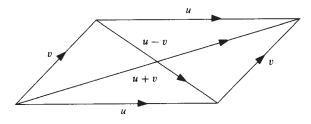
\includegraphics[scale=2.6]{figuras/leiparalelogramo.png}
\caption{Representação da lei do paralelogramo}
\end{figure}

\newpage

\noindent
Vamos calcular $\norm{u+v}^2$ e $\norm{u-v}^2:$
\[
\norm{u+v}^2 = \prin{u+v, u + v} = \textcolor{Blue}{\prin{u,u}} + \textcolor{Red}{\prin{u,v} + \prin{v,u}} + \textcolor{Green}{\prin{v,v}} = \textcolor{Blue}{\norm{u}^2} + \textcolor{Red}{2\prin{u,v}} + \textcolor{Green}{\norm{v}^2}
\]
\[
\norm{u-v}^2 = \prin{u-v, u - v} = \textcolor{Blue}{\prin{u,u}} - \textcolor{Red}{\prin{u,v} - \prin{v,u}} + \textcolor{Green}{\prin{v,v}} = \textcolor{Blue}{\norm{u}^2} - \textcolor{Red}{2\prin{u,v}} + \textcolor{Green}{\norm{v}^2}
\]
Somando as duas equações acima, obtemos
\[
\textcolor{Laranja}{\norm{u+v}^2}  + \textcolor{Purple}{\norm{u-v}^2} = \textcolor{Laranja}{\norm{u}^2 + \cancel{2\prin{u,v}} + \norm{v}^2}  + \textcolor{Purple}{\norm{u}^2 - \cancel{2\prin{u,v}} + \norm{v}^2} = 2 \norm{u}^2 + 2 \norm{v}^2.
\]
}

\exercicio{3} Se $K = \mathbb{R},$ mostre que, para $u, v \in V$, $\norm{u} = \norm{v}$ se, e somente se, $u + v$ e $u - v$ são
ortogonais. Discuta a afirmação para $K = \mathbb{C}.$
\solucao{
\dividiritens{
\task[\pers{a}]
\begin{itemize}
\item[$(\Rightarrow)$] Se $\norm{u} = \norm{v},$ então
\[
\norm{u} = \norm{v} \Rightarrow \norm{u}^2 = \norm{v}^2 \Rightarrow \norm{u}^2 - \norm{v}^2 = 0 \Rightarrow \norm{u}^2 \textcolor{Red}{+\prin{u,v}- \prin{u,v}}- \norm{v}^2 = 0 \Rightarrow \]\[ \norm{u}^2 -\prin{u,v}+ \prin{v,u}- \norm{v}^2 = 0 \Rightarrow \prin{u+v,u-v} = 0
\]
Logo, $u + v$ e $u - v$ são ortogonais.
\item[$(\Leftarrow)$] Se $u+v,$ $u-v$ são ortogonais, então
\[\prin{u+v,u-v} = 0 \Rightarrow \textcolor{Green}{\prin{u,u}} - \prin{u,v} + \prin{v,u} - \textcolor{Blue}{\prin{v,v}} = 0 \Rightarrow \textcolor{Green}{\norm{u}^2} - \textcolor{Blue}{\norm{v}^2} = 0 \Rightarrow \norm{u} = \norm{v} \]
\end{itemize}

\noindent
Observe que em ambos os sentidos da demonstração utilizamos fortemente o fato de que $\prin{u,v} = \prin{v,u},$ e salientamos que isso só é verdade para espaços vetoriais reais.

\task[\pers{b}]  Se $K = \mathbb{C},$ temos que $\prin{u,v} = \overline{\prin{v,u}}.$ Assim, o resultado pode não ser válido. Com efeito, tome por exemplo $u = (3+i, 5, 7+2i, 7 -4\sqrt{2} i)$ e $v = (0, 5, 12, 0).$ Observe que $\norm{u} = \norm{v} = 13,$ mas $u + v = (3+i, 10,19+2i, 7 -4\sqrt{2} i)$ e $u-v = (3+i, 0, -5+2i, 7 -4\sqrt{2} i),$ e
\[
\prin{u+v,u - v} = (3+i)^2 + 10 \cdot 0 + (19+2i)(-5+2i) + (7 -4\sqrt{2} i)^2 = -74 + (34 - 56 \sqrt{2})i \neq 0 .
\]
}
}
\exercicio{4} Seja $V$ um espaço vetorial sobre um corpo $K.$
\dividiritens{
\task[\pers{a}] Se $K = \mathbb{C}$, mostre que vale a \emph{identidade de polarização complexa}, para todos $u, v \in V:$
\[
4 \prin{u,v} = \norm{u+v}^2 - \norm{u-v}^2 + i \norm{u+iv}^2 - i\norm{u-iv}^2
\]
\task[\pers{b}] Se $K = \mathbb{R}$, mostre que vale a \emph{identidade de polarização real}, para todos $u, v \in V:$
\[
4 \prin{u,v} = \norm{u+v}^2 - \norm{u-v}^2
\]
}
\solucao{
\dividiritens{
\task[\pers{a}] Utilizando o mesmo raciocínio do Exercício 2, temos
\[
\norm{u+v}^2 = \prin{u+v, u + v} = \textcolor{Blue}{\prin{u,u}} + \textcolor{Red}{\prin{u,v}} + \textcolor{red}{\prin{v,u}} + \textcolor{Green}{\prin{v,v}}
\]
\[
\norm{u-v}^2 = \prin{u-v, u - v} = \textcolor{Blue}{\prin{u,u}} - \textcolor{Red}{\prin{u,v}} - \textcolor{red}{\prin{v,u}} + \textcolor{Green}{\prin{v,v}}
\]
\[
\norm{u+iv}^2 = \prin{u+iv, u + iv} = \textcolor{Blue}{\prin{u,u}} - i\textcolor{Red}{\prin{u,v}} + i\textcolor{red}{\prin{v,u}} + \textcolor{Green}{\prin{v,v}}
\]
\[
\norm{u-iv}^2 = \prin{u-iv, u - iv} = \textcolor{Blue}{\prin{u,u}} + i\textcolor{Red}{\prin{u,v}} - i\textcolor{red}{\prin{v,u}} + \textcolor{Green}{\prin{v,v}}
\]
assim obtemos:
\[
\norm{u+v}^2 = \textcolor{Blue}{\prin{u,u}} + \textcolor{Red}{\prin{u,v}} + \textcolor{red}{\prin{v,u}} + \textcolor{Green}{\prin{v,v}}
\]
\[
-\norm{u-v}^2 = -\textcolor{Blue}{\prin{u,u}} + \textcolor{Red}{\prin{u,v}} + \textcolor{red}{\prin{v,u}} - \textcolor{Green}{\prin{v,v}}
\]
\[
i\norm{u+iv}^2 = i\textcolor{Blue}{\prin{u,u}} + \textcolor{Red}{\prin{u,v}} - \textcolor{red}{\prin{v,u}} + i\textcolor{Green}{\prin{v,v}}
\]
\[
-i\norm{u-iv}^2 = -i\textcolor{Blue}{\prin{u,u}} + \textcolor{Red}{\prin{u,v}} - \textcolor{red}{\prin{v,u}} - i\textcolor{Green}{\prin{v,v}}
\]
assim somando as quatro equações acima, obtemos:
\[
\norm{u+v}^2 - \norm{u-v}^2 + i \norm{u+iv}^2 - i\norm{u-iv}^2=4 \prin{u,v}.
\]

\task[\pers{b}] Utilizando o mesmo raciocínio do Exercício 2, temos
\[
\norm{u+v}^2 = \prin{u+v, u + v} = \textcolor{Blue}{\prin{u,u}} + \textcolor{Red}{\prin{u,v} + \prin{v,u}} + \textcolor{Green}{\prin{v,v}} = \textcolor{Blue}{\norm{u}^2} + \textcolor{Red}{2\prin{u,v}} + \textcolor{Green}{\norm{v}^2}
\]
\[
\norm{u-v}^2 = \prin{u-v, u - v} = \textcolor{Blue}{\prin{u,u}} - \textcolor{Red}{\prin{u,v} - \prin{v,u}} + \textcolor{Green}{\prin{v,v}} = \textcolor{Blue}{\norm{u}^2} - \textcolor{Red}{2\prin{u,v}} + \textcolor{Green}{\norm{v}^2}
\]
Subtraindo as duas equações acima, vem
\[
\textcolor{Laranja}{\norm{u+v}^2}  - \textcolor{Purple}{\norm{u-v}^2} = \textcolor{Laranja}{\norm{u}^2 + 2\prin{u,v} + \norm{v}^2}  - \textcolor{Purple}{\norm{u}^2 - 2\prin{u,v} + \norm{v}^2} =\]\[ \cancel{\norm{u}^2} + 2\prin{u,v} + \bcancel{\norm{v}^2} - \cancel{\norm{u}^2} + 2\prin{u,v} - \bcancel{\norm{v}^2} = 4 \prin{u,v}.
\]
}
}
\exercicio{5} Encontre uma base ortonormal de cada um dos seguintes subespaços $S$ e determine também, em cada caso, o subespaço $S^{\perp}.$ 
\dividiritens{
\task[\pers{a}] $S$ é o subespaço de $\mathbb{C}^3$ gerado pelos vetores $v_1 = (1, 0, i)$ e $v_2 = (2, 1, 1 + i),$ com o produto interno usual. 
\task[\pers{b}] $S = \{ (x,y,z) \in \mathbb{R}^3 | x + y + z = 0 \},$ com o produto interno usual.
\task[\pers{c}] $S = \{ p(t) \in \mathcal{P}_3 (\mathbb{R}) | tp^{\prime}(t) = p(t) \}$ e $\prin{p,q} = \displaystyle \int\limits_0^1 p(t)q(t) \dif t$
\task[\pers{d}] $S = \{ A \in \mathcal{M}_3(\mathbb{R}) | \tr(A) = 0 \}$ e $\prin{A,B} = \tr(AB^t).$
\task[\pers{e}] $S = \langle (1,-1,1) \rangle,$ com o produto interno usual.%S^{\perp} = \langle (0, 1, 1), (1,1,0) \rangle
}
\solucao{}
\exercicio{6}  Prove que se 
\[\abs{\prin{u,v}} = \norm{u} \norm{v},
\] então $u$ e $v$ são linearmente dependentes.
\solucao{}
\exercicio{7} Sejam $W$ um subespaço de $V$ e $v \in V.$ Um vetor $w \in W$ é uma \emph{melhor aproximação} para $v$ por
vetores em $W$ se \[\norm{v - w} \le \norm{v - u}, \mbox{ para todo } u \in W.\] Prove que
\dividiritens{
\task[\pers{a}] O vetor $w \in W$ é uma melhor aproximação para $v \in V$ por vetores em $W$ se, e somente
se, $v - w \in W^{\perp}.$
\task[\pers{b}] Se uma melhor aproximação para $v \in V$ por vetores em $W$ existe, então ela é única.
\task[\pers{c}] Se $\dim W < \infty$ então existe uma melhor aproximação para $v \in V$ por vetores em $W$ e ela é dada por $w = \displaystyle\sum\limits_{i=1}^k \prin{v,e_i} e_i,$ onde $\{e_1, \ldots, e_k\}$ é uma base ortonormal qualquer de $W.$
}

Tal vetor é chamado de \emph{projeção ortogonal de v em W.}
\solucao{}
\exercicio{8} Sejam $W$ um subespaço de $V$ e $v \in V.$ Seja $E \colon V \to V$ a função tal que $E(v) = w,$ a projeção
ortogonal de $v$ em $W.$ (Assuma que, para todo $v \in V,$ existe tal $w.$) Prove que 
\dividiritens{
\task[\pers{a}] $E$ é um operador linear em $V.$
\task[\pers{b}] $E$ é idempotente.
\task[\pers{c}] $\mbox{Im } E = W$ e $\Ker E = W^{\perp}.$
\task[\pers{d}] $V = W \oplus W^{\perp}.$
}
\solucao{}
\exercicio{9} Seja $W$ um subespaço de dimensão finita de $V.$ Existem, em geral, várias projeções cuja imagem é $W.$ Uma delas, a projeção ortogonal, tem a propriedade que $\norm{E(v)} \le \norm{v},$ para
todo $v \in V.$ Prove se $E \in \mathcal{L}(V)$ é uma projeção cuja imagem é $W$ e $\norm{E(v)} \le \norm{v},$ para todo $v \in V,$ então $E$ é a projeção ortogonal em $W.$
(\textbf{Sugestão:} Prove que $\prin{E(v), v - E(v)} = 0,$ para todo $v \in V$ se, e somente se, $\prin{u, E(v)} = 0,$
para todo $u \in \Ker E$ e $v \in V.$ )
\solucao{}
\exercicio{10}  Sejam $W$ um subespaço de dimensão finita de $V$ e $E$ a projeção ortogonal de $V$ em $W$. Prove que $\prin{E(v), u} = \prin{v, E(u)}$ para todos $u, v \in V.$
\solucao{}
\exercicio{11} Sejam $V$ e $W$ espaços vetoriais de mesma dimensão (finita) sobre $K$ e com produtos internos $\prin{,}_V$ e $\prin{,}_W,$ respectivamente. Seja $T : V \rightarrow W$ uma transformação linear. Prove que as
seguintes afirmações são equivalentes: 
\dividiritens{
\task[\pers{a}] $\prin{T(u), T(v)}_W = \prin{u,v},$ para todos $u,v \in V.$
\task[\pers{b}] $T$ leva \textbf{toda} base ortonormal de $V$ em uma base ortonormal de $W.$
\task[\pers{c}] $T$ leva \textbf{uma} base ortonormal de $V$ em uma base ortonormal de $W.$
\task[\pers{d}] $\norm{T(v)}_W = \norm{v}_V$ para todo $v \in V.$
}
Tal $T$ é um \emph{isomorfismo de espaços com produto interno.}
\solucao{}
\exercicio{12} Uma matriz $A \in \mathcal{M}_n(K)$ é chamada \emph{ortogonal} se $AA^t = I_n$ e \emph{unitária} se $AA^{*} = I_n.$ Encontre um exemplo de uma matriz complexa unitária que não é ortogonal e um exemplo de uma matriz que é ortogonal e não é unitária.
\solucao{}
\exercicio{13} Seja $T \in \mathcal{L}(V)$ um isomorfismo de espaços com produto interno, isto é,
\[\prin{T(u), T(v)} = \prin{u,v},
\] para todos $u, v \in V.$ Prove que $T$ possui um adjunto e $T^{*} = T^{-1}.$ Prove que vale
também a recíproca, isto é, se $T$ possui um adjunto com $T^{*} = T^{-1},$ então $T$ é um isomorfismo de espaços com produto interno. Tal $T$ é chamado \emph{operador unitário} se $K = \mathbb{C}$ e \emph{ortogonal} se $K = \mathbb{R}.$
\solucao{$(\Rightarrow)$ Para provar que $T$ possui um adjunto, precisamos verificar que existe $T^* \in \mathcal{L}(V)$ tal que
\[
\prin{T(u), v} = \prin{u, T^{*}(v)}, \quad \forall u,v \in V
\]
Como $T$ é um isomorfismo, sabemos que existe $T^{-1} \in \mathcal{L}(V).$ Consideremos o vetor $v = T^{-1}(w).$ Daí, $\forall u, w \in V:$
\[
\begin{array}{rcl}
\prin{T(u), T(\textcolor{Green}{v})} = \prin{u,\textcolor{Green}{v}} &\Rightarrow& \prin{T(u), T(\textcolor{Green}{T^{-1}(w)})} = \prin{u,\textcolor{Green}{T^{-1}(w)}} \\&\Rightarrow& \prin{T(u), w} = \prin{u, T^{-1}(w)}.
\end{array}
\]
Logo, $T$ possui um adjunto, e $T^{*} = T^{-1}.$
\newline
$(\Leftarrow)$ Se $T \in \mathcal{L}(V)$ possui um operador adjunto $T^{*} \in \mathcal{L}(V),$ sabemos por definição que
\[
\prin{T(u), v} = \prin{u, T^{*}(v)}, \quad \forall u,v \in V
\]
Como $T^{*} = T^{-1},$ escrevendo $v = T(w),$ temos que
\[
\begin{array}{rcl}
\prin{T(u), v} = \prin{u, \textcolor{Blue}{T^{*}}(v)} &\Rightarrow& \prin{T(u), \textcolor{Violet}{v}} = \prin{u, \textcolor{Blue}{T^{-1}}(\textcolor{Violet}{v})} \\&\Rightarrow& \prin{T(u), \textcolor{Violet}{T(w)}} = \prin{u, \textcolor{Blue}{T^{-1}}(\textcolor{Violet}{T(w)})} \\&\Rightarrow& \prin{T(u), T(w)} = \prin{u, T^{-1}(T(w))} \\&\Rightarrow& \prin{T(u), T(w)} = \prin{u, w}.
\end{array}
\]
Logo, $T$ é um isomorfismo.
}
\solucao{}
\exercicio{14} Seja $T$ o operador linear em $\mathbb{C}^2$ (com o produto interno usual) definido por: $T(1, 0) = (1 +
i, 2)$ e $T(0, 1) = (i, i).$ Determine a matriz de $T^{*}$
em relação à base canônica de $\mathbb{C}^2$. Vale que
$TT^{*} = T^{*}T?$
\solucao{Seja $A \in \mathcal{M}_2(\mathbb{C})$ a matriz que representa $T.$ Pelas informações do enunciado, se
\[
A = \begin{pmatrix}
\alpha & \beta \\
\gamma & \delta
\end{pmatrix},
\]
devemos ter
\[
\begin{pmatrix}
\alpha & \beta \\
\gamma & \delta
\end{pmatrix} \begin{pmatrix}
1 \\ 0
\end{pmatrix} =  \begin{pmatrix}
1+i \\ 2
\end{pmatrix} \quad \mbox{e} \quad \begin{pmatrix}
\alpha & \beta \\
\gamma & \delta
\end{pmatrix} \begin{pmatrix}
0 \\ 1
\end{pmatrix} =  \begin{pmatrix}
i \\ i
\end{pmatrix}.
\]
Daí, segue que $\alpha = 1 + i, \gamma = 2, $ e $\beta = \delta = i.$ Portanto, a matriz de $T$ na base canônica de $\mathbb{C}^2$ é \[\begin{pmatrix}
1+i & i \\
2 & i
\end{pmatrix}.\]
Observe que a matriz adjunta $T^{*}$ corresponde ao hermitiano de $A,$ ou seja,
\[
[T^{*}]_{\mbox{can}} = A^{*} = A^{H} = \overline{A}^t.
\]
Logo, temos que a matriz procurada é
\[[T^{*}]_{\mbox{can}} = A^{*} = \overline{\begin{pmatrix}
1+i & i \\
2 & i
\end{pmatrix}}^t = \begin{pmatrix}
1-i & -i \\
2 & -i
\end{pmatrix}^t = \begin{pmatrix}
1-i & 2\\
-i & -i
\end{pmatrix}\]
Observe que
\[AA^{*} = \begin{pmatrix}
1+i & i \\
2 & i
\end{pmatrix}\begin{pmatrix}
1-i & 2\\
-i & -i
\end{pmatrix} = \begin{pmatrix}
3 & 3 +2i\\
3-2i & 5
\end{pmatrix}
\]
\[
A^{*}A = 
\begin{pmatrix}
1-i & 2\\
-i & -i
\end{pmatrix} \begin{pmatrix}
1+i & i \\
2 & i
\end{pmatrix} =
\begin{pmatrix}
6 & 1+3i\\
1-3i & 2
\end{pmatrix}
\]
Logo $TT^{*} \neq T^{*}T$ nesse caso, ou seja, $T$ não é um operador normal.
}
\exercicio{15} Seja $T$ um operador linear em $V$ que possui um adjunto $T^{*}.$
\dividiritens{
\task[\pers{a}] Mostre que $\Ker T^{*} = (\mbox{Im }T)^{\perp}$ e que $\mbox{Im }T^{*} \subset (\Ker T)^{\perp}.$
\task[\pers{b}] Mostre que se $\dim V < \infty,$ então $\mbox{Im }T^{*} = (\Ker T)^{\perp}.$
\task[\pers{c}] Seja $V = \mathcal{C}([0, 1], \mathbb{R})$ e $T \in \mathcal{L}(V)$ definida por: $f \longmapsto T(f),$, com $(T(f))(t) = t f(t)$ para
todo $t \in [0, 1].$ Determine $T^{*}$ e mostre que $\mbox{Im } T^{*} \neq (\Ker T)^{\perp}.$
}
\solucao{
\dividiritens{
\task[\pers{a}] Provemos que $\Ker T^{*} = (\mbox{Im }T)^{\perp}.$ Temos que
\[
\begin{array}{rcl}
  x \in \Ker T^{*}   &  \Leftrightarrow & T^{*}(x) = 0\\
     &  \Leftrightarrow & \prin{T^{*}(x),y} = 0, \ \forall y \in V\\
     &  \Leftrightarrow & \prin{x,T(y)} = 0, \ \forall y \in V\\
     &  \Leftrightarrow & x \perp \mbox{Im } T \\
     &  \Leftrightarrow & x \in (\mbox{Im }T)^{\perp}
\end{array}
\]
}

}

\exercicio{16} Seja $T \in \mathcal{L}(V).$ Prove que se $T$ é inversível, então $T^{*}$ é inversível e $(T^{*})^{-1} = (T^{-1})^{*}.$
\solucao{Se $T$ é inversível, então existe $T^{-1} \in \mathcal{L}(V)$ tal que $TT^{-1} = I.$ Desse modo, das propriedades da adjunção, temos que
\[
(TT^{-1})^{*} = I^{*} \Rightarrow (T^{-1})^{*} T^{*} = I
\]
Logo, $(T^{-1})^{*} \in \mathcal{L}(V)$ é tal que $(T^{-1})^{*} T^{*} = I.$ Portanto, $T^{*}$ é inversível.

Para mostrar que $(T^{*})^{-1} = (T^{-1})^{*},$ podemos seguir dois caminhos:
\begin{itemize}

\item Temos que
\[
I = I^{*}(TT^{-1})^{*} = (T^{-1})^{*}T^{*}.
\]
Logo, $\left(T^{-1}\right)^{*} = \left(T^{*}\right)^{-1}.$

\item Sabemos que $(T^{*})^{-1}T^{*} = I,$ então $((T^{*})^{-1}T^{*})^{*} = I^{*}.$ Das propriedades de $*,$ temos que $I^{*} = I,$ $(AB)^{*} = B^{*}A^{*}$ e $A^{**} = A.$ Daí,
\[
(\textcolor{Cerulean}{(T^{*})^{-1}} \textcolor{JungleGreen}{T^{*}})^{*} = \textcolor{RawSienna}{I^{*}} \Rightarrow
(\textcolor{JungleGreen}{(T^{*}})^{*} (\textcolor{Cerulean}{T^{*})^{-1}})^{*}  = \textcolor{RawSienna}{I} \Rightarrow \textcolor{Gray}{T^{**}} ((T^{*})^{-1})^{*} = I \Rightarrow \textcolor{Gray}{T} ((T^{*})^{-1})^{*} = I 
\]
Assim, concluímos que $((T^{*})^{-1})^{*}$ é a inversa de $T.$ Ou seja,
\[
T^{-1} = ((T^{*})^{-1})^{*} \Rightarrow (T^{-1})^{*} = (((T^{*})^{-1})^{*})^{*} \Rightarrow (T^{-1})^{*} = ((T^{*})^{-1})^{**}  \Rightarrow \boxed{(T^{-1})^{*} = (T^{*})^{-1}}
\]


    \item Sendo $T^{*}$ o adjunto de $T,$ sabemos por definição que
     \[\langle T(u),v \rangle = \langle u, T^*(v) \rangle \quad \forall u,v\in V\]

Então, substituindo $u$ por $T^{-1}(w),$ onde $w \in V,$ ficamos com
\[
\langle T(\textcolor{Green}{u}),v \rangle = \langle \textcolor{Green}{u}, T^*(v) \rangle \Rightarrow \langle T(\textcolor{Green}{T^{-1}(w)}),v \rangle = \langle \textcolor{Green}{T^{-1}(w)}, T^*(v) \rangle \Rightarrow \langle w, v \rangle = \langle T^{-1}(w), T^{*}(v) \rangle
\]
Por outro lado, para $T^{-1}$ e $x = T^{*}(v) \in V:$
\[
\langle \textcolor{Blue}{T^{-1}}(w),\textcolor{Magenta}{x} \rangle = \langle w, (\textcolor{Blue}{T^{-1}})^*(\textcolor{Magenta}{x}) \rangle \Rightarrow \langle \textcolor{Blue}{T^{-1}}(w),\textcolor{Magenta}{T^{*}(v)} \rangle = \]\[\langle w, (\textcolor{Blue}{T^{-1}})^*(T^{*}(v)) \rangle \Rightarrow  \langle T^{-1}(w),T^{*}(v) \rangle = \langle w, (\textcolor{Laranja}{TT^{-1}})^*(v) \rangle \Rightarrow  \]\[ \langle T^{-1}(w),T^{*}(v) \rangle = \langle w, \textcolor{Laranja}{I}^*(v) \rangle \Rightarrow  \langle T^{-1}(w),T^{*}(v) \rangle = \langle w, v \rangle  
\]
Daí, temos que
\[
\langle T^{-1}(w), T^{*}(v) \rangle = 
\] \textcolor{Red}{MelhorarEXPLICAÇÃO}
%https://math.stackexchange.com/questions/1006975/adjoint-operator-and-inverse
\end{itemize}
}
\exercicio{17}  Seja $E$ um operador linear em $V$ tal que $E^2 = E$ e tal que $E$ possui um adjunto $E^{*}.$ Prove que $E$ é autoadjunto se, e somente se $EE^{*} = E^{*}E.$ Prove também que, neste caso, $E$ é a projeção
ortogonal em $W = \mbox{Im }E.$
\solucao{
Se $E^2=E$ e $EE^*=E^*E$, então para todo $x$ temos o seguinte:
\[
\begin{array}{cl}
&\prin{E(x)-E^*E(x),E(x)-E^*E(x)}\\
=&\prin{E(x),E(x)}-\prin{E(x),\textcolor{Green}{E^*}E(x)}-\prin{\textcolor{Green}{E^*}E(x),E(x)}+\prin{\textcolor{red}{E^*}E(x),\textcolor{blue}{E^*}E(x)}\\
=&\prin{E(x),E(x)}-\prin{\textcolor{Green}{E}E(x),E(x)}-\prin{E(x),\textcolor{Green}{E}E(x)}+\prin{\textcolor{blue}{E}\textcolor{red}{E^*}E(x),E(x)}\\
=&\prin{E(x),E(x)}-\prin{EE(x),E(x)}-\prin{E(x),EE(x)}+\prin{\textcolor{red}{E^*}\textcolor{blue}{E}E(x),E(x)}\\
=&\prin{E(x),E(x)}-\prin{EE(x),E(x)}-\prin{E(x),EE(x)}+\prin{\textcolor{blue}{E}E(x),\textcolor{red}{E}E(x)}\\
=&\prin{E(x),E(x)}-\prin{E(x),E(x)}-\prin{E(x),E(x)}+\prin{E(x),E(x)}\\
=&0,
\end{array}
\]
assim:
\[
E(x)-E^*E(x)=0;
\]
logo:
\[
E=E^*E,
\]
portanto:
\[
E^*=(E^*E)^*=E^*E^{**}=E^*E=E.
\]
Agora, para $x\in V$, então para $y\in V$ temos:
\[
\begin{array}{rcl}
\prin{x-E(x),E(y)}&=&\prin{x,E(y)}-\prin{E(x),E(y)}\\&=&\prin{x,E(y)}-\prin{x,EE(y)}\\&=&\prin{x,E(y)}-\prin{x,E(y)}\\&=&0;
\end{array}
\]
logo $x-E(x)$ é ortogonal a $\mbox{Im }E$. Assim $E$ é a projeção ortogonal a $\mbox{Im E}.$
}

\exercicio{18} Sejam $V$ um espaço vetorial sobre $\mathbb{C}$ e $T \in \mathcal{L}(V).$ Prove que $T$ é autoadjunto se, e somente se $\prin{T(v), v} \in \mathbb{R},$ para todo $v \in V.$
\solucao{$(\Rightarrow)$ Seja $T$ um operador auto-adjunto. Então, sabemos que $T^{*} = T.$ Para mostrar que certo $z \in \mathbb{C}$ é real, basta verificar que $z = \overline{z}.$ Dado  $v \in V,$ tem-se que
\[
\langle T(v), v \rangle = \langle v, \textcolor{Brown}{T^{*}}(v) \rangle = \langle v, \textcolor{Brown}{T^{*}}(v) \rangle = \overline{\langle T(v),v \rangle} \Rightarrow \langle T(v), v \rangle \in \mathbb{R}
\]
$(\Leftrightarrow)$ Dado $v \in V,$ se $\prin{T(v), v} \in \mathbb{R}$, então temos que $\prin{T(v), v} = \overline{\prin{T(v), v}}.$ Assim,
\[
\langle T(v), v \rangle = \overline{ \langle T(v), v \rangle } = \overline{ \langle v, T^{*}(v) \rangle } = \langle T^{*}(v), v \rangle \Rightarrow \langle (T - T^{*})(v), v \rangle = 0 \quad \forall v \in V
\]
Como $V$ é um espaço vetorial sobre $\mathbb{C},$ temos que $T - T^{*},$ acarretando $T = T^{*}.$
}
\exercicio{19} Sejam $V$ um espaço vetorial sobre $\mathbb{C}$ e $T \in \mathcal{L}(V).$ Prove que se $\prin{T(v), v} = 0,$ para todo $v \in V,$ então $T = 0.$ Dê um exemplo para mostrar que o mesmo resultado não é necessariamente
verdadeiro se $V$ é um espaço vetorial sobre $\mathbb{R}.$ 
\solucao{Por hipótese, $\prin{T(v + w), v + w} = 0$ para quaisquer $v,w \in V.$ Assim,
\[
\prin{T(v + w), v + w} = 0 \Rightarrow \prin{T(v) + T(w), v + w} = 0 \Rightarrow  \textcolor{Laranja}{\prin{T(v), v}} + \prin{T(v), w} + \prin{T(w), v} + \textcolor{Laranja}{\prin{T(w), w}} \Rightarrow  \]\[ \textcolor{Laranja}{0} + \prin{T(v), w} + \prin{T(w), v} + \textcolor{Laranja}{0} \Rightarrow \prin{T(v), w} + \prin{T(w), v} = 0
\]
Note que $w$ é arbitrário na igualdade obtida acima.  Daí, podemos substituir $w$ por $iw,$ e usando que
\[
\prin{T(v), i w} = \overline{i} \prin{T(v), w} =  -i \prin{T(v), w} \quad \mbox{e} \quad \prin{T(iw),v} = \prin{iT(w), v} = i \prin{T(w), v},
\]
podemos verificar que
\[
\prin{T(v), \textcolor{Blue}{w}} + \prin{T(\textcolor{Blue}{w}), v} = 0 \Rightarrow \prin{T(v), \textcolor{Blue}{iw}} + \prin{T(\textcolor{Blue}{iw}), v} = 0 \Rightarrow - i \prin{T(v), w} + i \prin{T(w), v} = 0 \Rightarrow \]\[i(\prin{T(w), v} - \prin{T(v), w}) = 0 \Rightarrow \prin{T(w), v} - \prin{T(v), w} = 0
\]
Dessa forma, temos que
\[
\cancel{\prin{T(v), w}} + \prin{T(w), v} + \prin{T(w), v} - \cancel{\prin{T(v), w}} = 0 \Rightarrow 2\prin{T(w), v} = 0 \Rightarrow \boxed{\prin{T(w), v} = 0}
\]
Obtemos portanto que $\prin{T(w), v} = 0$ para quaisquer $v,w \in V.$ Vejamos que isso acarreta $T = 0.$

Faça $v = T(w).$ Então $\prin{T(w), T(w)} = 0$ e daí $T(w) = 0$ para todo $w \in V.$ Consequentemente, $T = 0.$

Observe que na resolução acima tivemos que considerar a unidade imaginária em certo momento. Vejamos que tal resultado não vale para espaços vetoriais sobre $\mathbb{R}.$ Considere o operador linear $T$ em $V = \mathbb{R}^2$ definido por $T(x,y) = (y,-x).$ Então, para todo $v = (v_1, v_2) \in \mathbb{R}^2,$ temos que
\[
\prin{\textcolor{Emerald}{T(v)}, v} = \prin{\textcolor{Emerald}{(-v_2, v_1)}, (v_1, v_2)} = -v_2v_1 + v_1v_2 = 0.
\]
Logo, $\prin{T(v),v} = 0$ para todo $v \in V,$ mas claramente $T \neq 0.$
}
\exercicio{20} Sejam $V$ um espaço vetorial sobre $\mathbb{C}$ e $T$ uma função de $V$ em $V$ tal que, para todos $u, v \in V,$ $\norm{T(u) - T(v)} = \norm{u-v}$ e $T(iv) = iT(v).$ Prove que $T$ é linear e que $\norm{T(v)} = \norm{v},$ para todo $v \in V.$

\solucao{}
\exercicio{21} Seja $T$ um operador linear em $V$ tal que $T$ admite um adjunto. Prove que se $T^{*}T = 0$ então $T = 0.$

\solucao{
Vamos mostrar algo melhor. Provaremos que, para cada $x\in V$, se $T^*T(x)=0$, então $T(x)=0$. De fato, se $T^*T(x)=0$, então:
\[
\prin{T(x),T(x)}=\prin{x,T^*T(x)}=\prin{x,0}=0,
\]
aí $T(x)=0$.
}

\exercicio{22} Seja $A \in \mathcal{M}_n(\mathbb{C}).$ Mostre que $A$ se escreve de modo único como $A = B + iC,$ onde $B$ e $C$ são matrizes autoadjuntas.
\solucao{Façamos 
\[
B = \frac{A + A^{*}}{2} \quad \mbox{e} \quad C = \frac{A - A^{*}}{2i}.
\]
Então
\[
\textcolor{Emerald}{B} + i\textcolor{Cyan}{C} = \textcolor{Emerald}{\frac{A + A^{*}}{2}} + i\textcolor{Cyan}{\frac{A - A^{*}}{2i}} = \frac{A + A^{*}}{2} + \frac{A - A^{*}}{2} = \frac{2A}{2} = A.
\]
Além disso, 
\[
B^{*} = \left(  \frac{A + A^{*}}{2} \right)^{*} =  \frac{A^{*} + A^{**}}{2}  =  \frac{A^{*} + A}{2} = B
\]
e
\[
C^{*} = \left( \frac{A - A^{*}}{2i} \right)^{*} =  \frac{A^{*} - A^{**}}{\overline{2i}} =  - \frac{A^{*} - A}{2i} =  \frac{A - A^{*}}{2i} = C, 
\]
ou seja, $B$ e $C$ são matrizes auto-adjuntas.
}
\exercicio{23}
Sejam $S, T \in \mathcal{L}(V).$ Suponha que $S$ e $T$ admitem adjuntas.

\dividiritens{
\task[\pers{a}] Mostre que se $S$ e $T$ são autoadjuntas, então $ST$ é autoadjunta se, e somente se, $ST = TS.$ 
\task[\pers{b}] Encontre duas matrizes $S$ e $T$ autoadjuntas tais que $ST$ não é autoadjunta.
\task[\pers{c}] Prove que $T^{*}T$ é autoadjunta.
\task[\pers{d}] Se $T$ é autoadjunta, mostre que $S^{*}TS$ é autoadjunta.
\task[\pers{e}] Mostre que se $S$ e $T$ são autoadjuntas, então $ST + TS$ é autoadjunta.
}

\solucao{\dividiritens{
\task[\pers{a}] Se $S$ e $T$ são autoadjuntas, então $S = S^{*}$ e $T = T^{*}.$ 
\newline
$(\Rightarrow)$ Se $ST$ é autoadjunta, então \[(ST)^{*} = \textcolor{Red}{S}\textcolor{Magenta}{T} = \textcolor{Red}{S^{*}}\textcolor{Magenta}{T^{*}} (TS)^{*}
\]
Portanto, da unicidade do operador adjunto, temos
\[
(ST)^* - (TS)^{*} = 0 \Rightarrow (ST - TS)^{*} = 0 \Rightarrow ST - TS = 0 \Rightarrow ST = TS. 
\]

$(\Leftrightarrow)$ Se $ST = TS,$ então
\[
(ST)^{*} = (TS)^{*} \Rightarrow (ST)^{*} = \textcolor{Red}{S^{*}}\textcolor{Magenta}{T^{*}} \Rightarrow  (ST)^{*} = \textcolor{Red}{S}\textcolor{Magenta}{T}.
\]
Portanto, $ST$ é autoadjunta.
\task[\pers{b}] Considere
\[
S = \begin{bmatrix}
1 & 0 \\ 0 & 0
\end{bmatrix} \quad \mbox{e} \quad T = \begin{bmatrix}
1 & 0 \\ 0 & 1 
\end{bmatrix} 
\]
Então $ST = \begin{bmatrix}
0 &1 \\ 0 & 0
\end{bmatrix}$ não é autoadjunta.
\newline
Outro exemplo: Sejam $T, S \in \mathcal{L}(\mathbb{R}^2),$ dadas por
\[
T(x,y) = (x+2y, 2x) \quad \mbox{e} \quad S(x,y)  = (y, x+y)
\]
As matrizes que representam $T$ e $S$ na base canônica (que é ortonormal) são
\[
A = \begin{bmatrix}
1 & 2 \\
2 & 0 
\end{bmatrix} \quad \mbox{e} \quad B = \begin{bmatrix}
0 & 1 \\
1 & 1
\end{bmatrix},
\]
respectivamente. Observe que $T$ e $S$ são autoadjuntos pois $A$ e $B$ são matrizes hermitianas. Temos que
\[
AB = \begin{bmatrix}
2 &3 \\ 0 & 2
\end{bmatrix}.
\]
Essa matriz não é hermitiana. Como a base canônica é ortonormal, então $TS$ não é autoadjunta.

\task[\pers{c}] Se $T$ é autoadjunta, então
\[
T^{*}T = TT^{*}
\]
Pelo item (a), tomando $S = T^{*},$ segue que $T^{*}T$ é autoadjunta.
\task[\pers{d}] Se $T$ é autoadjunta, então $T^{*} = T.$ Logo,
\[
\left(S^*TS\right)^{*} = \left(S^*(TS)\right)^{*} = (TS)^{*} S^{**} = S^{*}\textcolor{Green}{T^{*}}S = S^{*}\textcolor{Green}{T}S.
\]

\task[\pers{e}] Vamos provar $ST + TS$ é autoadjunta pela definição, ou seja, mostraremos que para todo $u,v \in V,$ 
\[
\prin{(ST + TS)(u), v} = \prin{u, (ST + TS)(v)}
\]
Para isso, lembrando que $T^{*} = T$ e $S^{*} = S,$ vemos que
\[
\begin{array}{rcl}
\prin{(ST+TS)(u),v} & = & \prin{(ST)(u),v} + \prin{(TS)(u), v} \\
& =&  \prin{S(\textcolor{Mahogany}{T(u)}),v} + \prin{T(\textcolor{Mahogany}{S(u)}), v} \\
& =&  \prin{\textcolor{Mahogany}{T(v)},\textcolor{Green}{S^{*}}(v)} + \prin{\textcolor{Mahogany}{S(u)}, \textcolor{Blue}{T^{*}}(v)} \\
& =&  \prin{T(v),\textcolor{Green}{S}(v)} + \prin{S(u), \textcolor{Blue}{T(v)}} \\
&=& \prin{u,  \textcolor{Blue}{T^{*}}(S(v))} + \prin{u, \textcolor{Green}{S^{*}}(T(v))} \\
&=& \prin{u,  \textcolor{Blue}{T}(S(v))} + \prin{u, \textcolor{Green}{S}(T(v))} \\
&=& \prin{u,(TS)(v)} + \prin{u, (ST)(v)} \\
& = & \prin{u, (ST + TS)(v)}
\end{array}
\]
Portanto, $\prin{(ST+TS)(u),v} =  \prin{u, (ST + TS)(v)},$ e $ST + TS$ é autoadjunta.
}
}

\exercicio{24} Seja $V$ um espaço vetorial com dimensão finita e seja $T \in \mathcal{L}(V)$ normal. Mostre que
\dividiritens{
\task[\pers{a}] Se $T$ é nilpotente, então $T = 0.$
\task[\pers{b}] Se $T$ é idempotente, então $T^{*} = T.$
\task[\pers{c}] Se $T^3 = T^2,$ então $T$ é idempotente.
\task[\pers{d}] Se $T^{8} = T^{7},$ $T$ é autoadjunto e idempotente.
}

\solucao{
\dividiritens{
\task[\pers{a}] Seja $T$ normal nilpotente. Então, existe um inteiro positivo $k$ tal que $T^k = 0.$ Vamos provar por indução que $T = 0.$ Se $k = 1,$ o resultado é trivial.

\medskip
\noindent
Suponha $k > 1$ e que o caso $k - 1$ funcione. Tome $B = T^{k-1}.$ Note que, como $T$ é normal, então $B$ também é normal.

\medskip
\noindent
Para um vetor $x \in V,$ vamos calcular a norma do vetor $B^{*}Bx$ como segue:
\[
\begin{array}{rcl}
\norm{B^*Bx} &=& \prin{B^*Bx,B^{*}Bx} \\
&=& \prin{Bx,B^{**} B^{*} Bx} \\
&  = & \prin{x,B^* \textcolor{TealBlue}{BB^{*}}Bx} \\
&  = & \prin{x,B^* \textcolor{TealBlue}{B^{*}B}Bx} \\
&=& \prin{x,(B^{*})^2B^2x}\\
&=& 0,
\end{array}
\]
pois $B^2 = T^{2k-2} = 0,$ já que $k \ge 2$ implica $2k-2 \ge k.$ Daí, temos que $B^*Bx = 0$ para todo $x \in V.$

\medskip
\noindent
Assim,
\[
\norm{Bx} = (Bx)^{*}(Bx) = x^*B^*Bx = 0, \quad \forall x \in V.
\]
Consequentemente, $B = 0.$

\medskip
\noindent
Pela hipótese de indução, $T^{k-1} = 0$ implica $T = 0.$ Portanto $T$ é o operador nulo.

\task[\pers{b}] Se $T$ é idempotente, então sabemos que $T^2 = T.$ Sendo normal, sabemos também que $T^*T = TT^*.$ Se $T^{*}T = 0,$ pelo Exercício 21, temos que $T = 0,$ que claramente é autoadjunto. 

\medskip
\noindent 
Consideremos agora $T^{*}T \neq 0.$ Então, observe que
\[
(T - T^{*})(T^{*}T) = T\textcolor{PineGreen}{T^{*}T} - T^{*}T^{*}T = T\textcolor{PineGreen}{TT^*} - \textcolor{ProcessBlue}{(T^2)}^{*}T =  \textcolor{ProcessBlue}{T^2}T^* - \textcolor{ProcessBlue}{T}^{*}T =   \textcolor{ProcessBlue}{T}T^* - \textcolor{PineGreen}{T^{*}T} =   \textcolor{ProcessBlue}{T}T^* - \textcolor{PineGreen}{TT^{*}} = 0
\]
Concluímos portanto que $(T - T^{*})(T^{*}T) = 0.$ Como $T^{*}T \neq 0,$ segue que $T - T^{*} = 0,$ acarretando $T = T^{*}.$
  \task[\pers{c}] Como $T$ é normal, pelo Teorema Espectral, existe uma base ortonormal $\{e_1, e_2, \ldots, e_n \}$ de $V$ consistindo de autovetores de $T.$ Sejam $\lambda_1, \ldots, \lambda_n$ os correspondentes autovalores. Então,
  \[
  T(e_j) = \lambda_j e_j,
  \]
  para $j = 1, \ldots, n.$ Aplicando $T$ uma quantidade adequada de vezes em ambos os membros da equação acima, temos que
\[
T^3(e_j) = \lambda_j^3e_j \quad \mbox{e} \quad T^2(e_j) = \lambda_j^{2}e_j.
\]
Dessa forma,
\[
T^3(e_j) = T^2(e_j) \Rightarrow \lambda_j^3e_j = \lambda_j^{2}e_j \Rightarrow \lambda_j^3 = \lambda_j^2 \Rightarrow \lambda_j^2(\lambda - 1) = 0
\]
Isso implica que $\lambda_j$ vale $1$
 ou $0.$ Em particular, todos os autovalores de $T$ são reais. A matriz de $T$ com respeito à base ortonormal $\{e_1, \ldots, e_n \}$ será a matriz diagona com $\lambda_1, \ldots, \lambda_n$ na diagonal. Esta matriz claramente é equivalente à sua transposta conjugada, e portanto é hermitiana. Daí, $T = T^{*}.$ %Consequentemente, $T$ é autoadjunto.
 Aplicando $T$ em ambos os membros na equação obtida inicialmente, ficamos com
 \[
 T^2(e_j) = \textcolor{Maroon}{\lambda^2_j} e_j = \textcolor{Maroon}{\lambda_j} e_j = T(e_j),
 \]
 onde utilizamos que $\lambda_j^2 = \lambda_j,$ afinal $\lambda_j$ vale $0$ ou $1.$ Como $T^2$ e $T$ coincidem numa base, então devem ser iguais. Logo, $T^2 = T,$ e $T$ é idempotente.
 \task[\pers{d}] Um raciocínio análogo ao do item (c)  permite concluir que $T$  é autoadjunto e idempotente. Em geral, usando uma argumentação similar, pode-se provar que todo operador normal para o qual existe um inteiro positivo $k \ge 1$ tal que $T^{k+1} = T^k$ é autoadjunto e idempotente.
 }
}

\exercicio{25} Seja $T$ um operador qualquer de um espaço com produto interno complexo $V$ de dimensão finita. Então $T$ pode ser representado por uma matriz triangular em relação a alguma base ortonormal de $V.$

\solucao{ Vamos utilizar indução na dimensão $n$ de $V.$ Se $\dim V = 1,$ é claro que a afirmação do teorema é válida. Suponhaentão, que $\dim V  = n > 1$ e que o teorema seja válido para operadores de espaços complexos de dimensão $n - 1.$
Dado que $V$ é um espaço vetorial complexo, $T$ tem, ao menos, um autovalor e, portanto, um autovetor não nulo $v$. Seja $W = \prin{v}$ o
subespaço de $V$ gerado por $v$ e seja $u_1$ um vetor unitário de $W.$ Então $u_1$ é um autovetor de $T$ e temos $T(u_1) = a_{11}u_1.$ Sabemos que $V = W \oplus W^{\perp}.$ Denotemos por $E_{W^{\perp}}$ a projeção ortogonal de $V$ sobre $W^{\perp}$. Claramente, é invariante
pelo operador $ET.$\footnote{Não é o Eduardo Tengan!} Por indução, existe uma base ortonormal $\{u_2, \ldots, u_n\}$ de $W^{\perp}$ tal que, para $i =  2, \ldots, n,$
\[
ET(u_i) = a_{i2}u_2 + a_{i3}u_3 + \ldots + a_{ii}u_i = \sum\limits_{j = 2}^i a_{ij}u_j 
\]
Observe que $\{u_1, u_2, \ldots, u_n\}$ é uma base ortonormal de $V.$ Como $E$ é a projeção ortogonal de $V$ sobre $W^{\perp},$ decorre que
\[
T(u_i) = a_{i1}u_1 + a_{i2}u_2 + a_{i3}u_3 + \ldots + a_{ii}u_i = \sum\limits_{j = 1}^i a_{ij}u_j 
\]
para $i=  2, \ldots, n.$ Como já temos que $T(u_1) = a_{11} u_1,$ temos que $T$ pode ser representado por uma matriz triangular em relação a alguma base ortonormal de $V.$
}


\exercicio{26} Um operador linear $T \in \mathcal{L}(V)$ é \emph{não negativo} (\emph{positivo}) se $T$ é autoadjunto e $\prin{T(v), v} \ge 0$ ($\prin{T(v), v} > 0$), para todo $v \in V.$ 
\dividiritens{
\task[\pers{a}] Se a dimensão de $V$ é finita e $T$ é não negativo, mostre que as autovalores de $T$ são números reais não negativos. 

\task[\pers{b}] Mostre que $T$ é não negativo se, e somente se, existe $S \in \mathcal{L}(V)$ não-singular tal que $T = S^{*}S.$
}

\solucao{
\dividiritens{
\task[\pers{a}]

Vamos 
\task[\pers{b}] $(\Rightarrow)$ Se $T$ é não-negativo (positivo), então $T^{*} = T$ e $\prin{T(v), v} \ge 0$ ($\prin{T(v), v} > 0$), para todo $v \in V.$

Como $T$ é autoadjunto, existe uma base ortonormal $\{e_1, \ldots, e_n\}$ consistindo de autovetores de $T.$ Escrevamos $T(e_i) = \lambda_ie_1.$ Pelo Exercício 25, $\lambda_i$ são reais para $i = 1, \ldots, n.$ Vejamos que $\lambda_i$ não podem ser negativos. Para cada $i,$ temos que
\[
0 \le \prin{\textcolor{Green}{T(u_i)}, u_i} =  \prin{\textcolor{Green}{\lambda_i u_i}, u_i} = \lambda_i \prin{u_i, u_i}
\]
\[
(0 \le \prin{\textcolor{Green}{T(u_i)}, u_i} =  \prin{\textcolor{Green}{\lambda_i u_i}, u_i} = \lambda_i \prin{u_i, u_i})
\]
Assim, $\prin{u_i, u_i} \ge 0$ ($\prin{u_i, u_i} > 0$), o que acarreta $\lambda_i \ge 0$ ($\lambda_i > 0$).


$(\Leftarrow)$ Se existe $S \in \mathcal{L}(V)$ não-singular tal que $T = S^{*}S,$ então $S(v) \neq 0.$ Logo, $\prin{S(u), S(u)}$ é não-negativo (positivo). Vamos mostrar que os autovalores de $T$ são reais e positivos, o que implica $T$ não-negativo (positivo). 

Para tanto, seja $\lambda$ um autovalor de $T$ e $v$ um autovetor associado. Então, $T(v) = \lambda v.$ Daí, temos que
\[
\prin{\textcolor{RawSienna}{T(v)},v} = \prin{\textcolor{RawSienna}{\lambda v},v} = \lambda \prin{v,v},
\]
mas também
\[
\prin{\textcolor{Blue}{T}(v),v} = \prin{\textcolor{Blue}{S^{*}S}(v),v} = \prin{S(v), S(v)}
\]
Como $\prin{v,v}$ e $\prin{S(v), S(v)}$ são não-negativos (positivos), temos que $\lambda$ é não-negativo (positivo), pois $\lambda = \frac{\prin{S(v), S(v)}}{\prin{v,v}}.$
}
}

\textcolor{Red}{Questões Suplementares}

\exercicio{31} Considere o seguinte subespaço de $\mathbb{R}^3:$
\[
W = \{ (x,y,z) \in \mathbb{R}^3 |x + 2y - 3z = 0, x - 2y + z = 0 \}
\]
\dividiritens{
\task[\pers{a}] Descreva o operador de projeção ortogonal de $V$ em $W.$
\task[\pers{b}] Verifique que $\mathbb{R}^3 = W \oplus W^{\perp}.$ 
}
\solucao{}
\exercicio{32} Seja $\mathcal{F}$ o espaço vetorial das funções reais com o produto interno usual, e considere os conjuntos
%https://www.ime.unicamp.br/~marcia/AlgebraLinear/Arquivos%20PDF/exemplos_subespacos.pdf
\[
S_p = \{ f \mid f(x) = f(-x) \} \quad \mbox{e} \quad S_i = \{ f \mid f(x) = -f(-x) \}
\]
\dividiritens{
\task[\pers{a}] Verifique que $S_i$ e $S_p$ são subespaços vetoriais de $\mathcal{F}.$
\task[\pers{b}] Descreva os operadores de projeção ortogonal de $\mathcal{F}$ em $S_i$ e em $S_p.$
\task[\pers{c}] Encontre subespaços $W_1$ e $W_2$ de $\mathcal{F}$ tais que \[\mathcal{F} = S_i \oplus W_1 \quad \mbox{e} \quad \mathcal{F} = S_p \oplus W_2 \]
\task[\pers{d}] Conclua que $\mathcal{F} = S_p \oplus S_i.$%http://www.uel.br/projetos/matessencial/superior/alinear/somadir.htm
%http://vectorsandgeometry.wikidot.com/3-5-exemplos-resolvidos-com-interseccao
}

\solucao{}

\exercicio{33} (Decomposição QR) A \emph{Decomposição QR} de uma matriz $A \in \mathcal{M}_n(K)$ consiste em escrever a matriz $A$ como um produto $QR,$ onde $Q$ é uma matriz ortogonal (se $K = \mathbb{R}$) ou unitária (se $K = \mathbb{C}$) e $R$ é uma matriz triangular superior. Tal decomposição é importante para o método dos mínimos quadrados e é base para algoritmos computacionais de cálculo de autovalores de uma matriz. 
\dividiritens{
\task[\pers{a}] Prove que toda matriz $A \in \mathcal{M}_n(K)$ admite uma decomposição $QR.$
\task[\pers{b}] Encontre a decomposição QR das seguintes matrizes:
\begin{itemize}
    \item[\textbf{($\alpha$)}] $A = \begin{pmatrix}
  12 & -51 &   4 \\
   6 & 167 & -68 \\
  -4 &  24 & -41
\end{pmatrix}$
    \item[\textbf{($\beta$)}]
\end{itemize}
}
%https://pt.wikipedia.org/wiki/Decomposi%C3%A7%C3%A3o_QR
%https://www.ufrgs.br/reamat/AlgebraLinear/livro/s13-o_processo_de_ortogonalizax00e7x00e3o_de_gramx2013schmidt.html
\solucao{}

\exercicio{34} Considere  $T_2 \in \mathcal{L}(\mathbb{R}^2)$ e $T_3 \in \mathcal{L}(\mathbb{R}^3),$ dadas respectivamente por
\[
T_2(x,y) = (x+3y, 3x+2y) \quad \mbox{e} \quad T_3(x,y,z) = (2x+7y+8z, 7x+3y+7z, 8x+7y+5z.
\]
\dividiritens{
\task[\pers{a}] Escreva as matrizes de $T_2$ e $T_3$ nas bases canônicas de $\mathbb{R}^2$ e $\mathbb{R}^3,$ respectivamente.
\task[\pers{b}] Encontre $T_2^{*}$ e $T_3^{*},$ e verifique que $T_2$ e $T_3$ são autoadjuntos.

Sabe-se que $\mathcal{B}_2 = \{ (1,1), (1,0) \}$ é uma base para $\mathbb{R}^2,$ e  $\mathcal{B}_3 = \{ (1,1,-1), (2,-1,0), (3,2,0) \}$ é uma base para $\mathbb{R}^3.$

\task[\pers{c}] Encontre as matrizes que representam $T_2$ e $T_3$ nessas bases.
\task[\pers{d}] Encontre as matrizes que representam $T_2^{*}$ e $T_3^{*}$ nessas bases e observe que ssas matrizes não são hermitianas. Isso entra em contradição com o fato de $T_2$ e $T_3$ serem autoadjuntas?
%$\mathcal{B}_2 = \{ (2,-1), (-3,2) \}$ 
}
\solucao{}

\exercicio{35} Suponha que $T$ é um operador normal em $V$ e $3$ e $4$ são seus autovalores. Prove que existe um vetor $v \in V$ tal que $\norm{v} = \sqrt{2}$ e $\norm{T(v)} = 5.$
\solucao{Sejam $u$ e $v$ os autovetores de $T$ com respeito aos autovalores $3$ e $4,$ respectivamente. Então,
\[
T(u) = 3u \quad \mbox{e} \quad T(w) = 4w.
\]
Trocando $u$ por $\frac{u}{\norm{u}}$ e $w$ por $\frac{w}{\norm{w}},$ podemos assumir sem perda de generalidade que $\norm{u} = \norm{w} = 1.$ 

Como $T$ é normal, $u$ e $w$ são ortogonais. O Teorema de Pitágoras implica que
\[
\norm{u + w} = \sqrt{\norm{u}^2 + \norm{w}^2} = \sqrt{2},
\]
e também
\[
\norm{T(u+w)} = \norm{T(u) + T(w)} = \norm{3u + 4w} = \sqrt{9 \norm{u}^2 + 16 \norm{v}^2} = 5.
\]
Tomando $v = u + w,$ obtemos um vetor $v$ tal que $\norm{v} = \sqrt{2}$ e $\norm{T(v)} = 5,$ como pedido pelo enunciado.
}
\newpage
\section{\textcolor{Floresta}{Lista 5,5}}

\subsection*{Espaços com produto interno}

   \exercicio{1} Determine quais das funções $\prin{,} \colon \mathbb{R}^4 \to \mathbb{R}$ abaixo definem um produto interno em $\mathbb{R}^4:$ 
\dividiritens{
\task[\pers{a}] $\prin{(a,b,c,d), (x,y,z,w)} = ax + 2by + 5cz + dw;$
\task[\pers{b}] $\prin{(a,b,c,d), (x,y,z,w)} = ax - by + cz + 3dw;$
\task[\pers{c}] $\prin{(a,b,c,d), (x,y,z,w)} = ay + 2bx + cz + dw;$
\task[\pers{d}] $\prin{(a,b,c,d), (x,y,z,w)} = ax + 5cz + dw;$
\task[\pers{e}] $\prin{(a,b,c,d), (x,y,z,w)} = ax + 2b + 5z + dw.$
}
\solucao{
Para resolver essa questão, podemos utilizar duas técnicas diferentes:
\begin{itemize}
    \item Verificando se os axiomas de produto interno são satisfeitos:
    \dividiritens{
    \task[\pers{a}] Temos que
    \newline 
    $\clubsuit$ $\prin{u+v,w} = \prin{u,w} + \prin{v,w}.$ 
        
        Sejam $u = (u_1, u_2, u_3, u_4), v = (v_1, v_2, v_3, v_4), w = (w_1, w_2, w_3, w_4) \in \mathbb{R}^4.$ Então
        \[
        \begin{array}{rcl}
        \prin{u +v,w} &=& \prin{\textcolor{Green}{(u_1 + v_1, u_2 + v_2, u_3 + v_3, u_4 + v_4)}, \textcolor{Blue}{(w_1, w_2, w_3, w_4)}} \\
        &=& \textcolor{Green}{(u_1+v_1)}\textcolor{Blue}{w_1} + 2\textcolor{Green}{(u_2+v_2)} \textcolor{Blue}{w_2} + 5 \textcolor{Green}{(u_3+v_3)}\textcolor{Blue}{w_3}+\textcolor{Green}{(u_4+v_4)}\textcolor{Blue}{w_4} \\ 
        &=& u_1w_1 +v_1w_1 + 2u_2w_2 + 2v_2w_2 + 5u_3w_3 + 5v_3w_3 + u_4w_4 + v_4w_4 \\ 
        &=& u_1w_1+ 2u_2w_2+5u_3w_3+ u_4w_4 + v_1w_1+ 2v_2w_2+5v_3w_3+ v_4w_4 \\ &=& \prin{(u_1,u_2,u_3,u_4),(w_1,w_2,w_3,w_4)} + \prin{(v_1,v_2,v_3,v_4),(w_1,w_2,w_3,w_4)} \\
        &=& \prin{u,w} + \prin{v,w}
        \end{array}
        \]
        \newline
$\textcolor{Red}{\varheart}$ $\prin{\alpha u, v} = \alpha \prin{u,v},$

Sejam $u = (u_1, u_2, u_3, u_4), v = (v_1, v_2, v_3, v_4) \in \mathbb{R}^4$ e $\alpha \in \mathbb{R}.$ Temos:
\[
\begin{array}{rcl}
\prin{\alpha u, v} &=& \prin{\textcolor{Green}{(\alpha u_1, \alpha u_2, \alpha u_3, \alpha u_4)}, \textcolor{Blue}{(v_1,v_2, v_3, v_4)}} \\
&=&\textcolor{Green}{\alpha u_1} \textcolor{Blue}{v_1} + 2\textcolor{Green}{\alpha u_2} \textcolor{Blue}{v_2} + 5\textcolor{Green}{\alpha u_3} \textcolor{Blue}{v_3} + \textcolor{Green}{\alpha u_4} \textcolor{Blue}{v_4} \\ &=& \alpha (u_1v_1+ 2u_2v_2+5u_3v_3+ u_4v_4) \\ &=& \alpha \prin{(u_1,u_2, u_3, u_4), (v_1,v_2, v_3, v_4)} \\ &=& \alpha \prin{u,v}
\end{array}
\]
\newline
$\spadesuit$ $\prin{u,v} = \prin{v,u}.$
Sejam $u = (u_1, u_2, u_3, u_4), v = (v_1, v_2, v_3, v_4) \in \mathbb{R}^4.$ Então
\[
\begin{array}{rcl}
\prin{u,v} &=& \prin{\textcolor{Green}{(u_1, u_2, u_3, u_4)}, \textcolor{Blue}{(v_1, v_2, v_3, v_4)} } \\
&=&\textcolor{Green}{u_1} \textcolor{Blue}{v_1} + 2\textcolor{Green}{ u_2} \textcolor{Blue}{v_2} + 5\textcolor{Green}{ u_3} \textcolor{Blue}{v_3} + \textcolor{Green}{ u_4} \textcolor{Blue}{v_4} \\
&=& v_1u_1 + 2v_2u_2 + 5v_3u_3 + v_4u_4 \\
&=& \prin{(v_1, v_2, v_3, v_4),(u_1, u_2, u_3, u_4)} \\
&=& \prin{v,u}
\end{array}
\]
\newline
$\textcolor{Red}{\vardiamond}$ $\prin{u,u} \ge 0; \prin{u,u} = 0 \Leftrightarrow u = 0.$ 

Seja $u = (u_1, u_2, u_3, u_4) \in \mathbb{R}^4.$ Então
\[
\prin{u,u} = \prin{(u_1, u_2, u_3, u_4),(u_1, u_2, u_3, u_4)} = u_1^2 +2u_2^2 + 5u_3^2 + u_4^2 \ge 0
\]
Além disso, 
\[
\prin{u,u} = 0 \Leftrightarrow u_1^2 +2u_2^2 + 5u_3^2 + u_4^2 = 0 \Leftrightarrow u = 0.
\]

Logo, temos que $\prin{(a,b,c,d), (x,y,z,w)} = ax + 2by + 5cz + dw$ é um produto interno em $\mathbb{R}^4.$

    \task[\pers{b}]
    
    
    \item Argumentando via matrizes, escrevendo o produto interno utilizando a notação matricial. 
    
    
    \task[\pers{a}] Podemos escrever
    \[
    \prin{(a,b,c,d), (x,y,z,w)} = u^t A v = (a,b,c,d) \begin{pmatrix}
    1 & 0 & 0 & 0 \\
    0 & 2 & 0 & 0 \\
    0 & 0 & 5 & 0 \\
    0 & 0 & 0 & 1 \\
    \end{pmatrix} \begin{pmatrix}
    x\\ y\\ z \\ w
    \end{pmatrix}.
    \]
    Como $A$ é real e simétrica, basta mostrar que $A$ é positiva definida. Se uma matriz é positiva definida, então é possível reduzí-la a uma matriz diagonal que possui todas as entradas na diagonal positivas. Claramente $A$ é uma matriz diagonal, e todas suas entradas na diagonal são positivas. Logo, $A$ é positiva definida, e $\prin{(a,b,c,d), (x,y,z,w)} = ax + 2by + 5cz + dw$ é um produto interno em $\mathbb{R}^4.$
    
    \task[\pers{b}]
    }
    
\end{itemize}


}

\exercicio{2} Considere a função $\prin{,} \colon \mathbb{C}^2 \to \mathbb{C}^2$ dada por
\[
\prin{u,v} = x_1\overline{y_1} + (1+i)x_1\overline{y_2} + (1-i)x_2\overline{y_1} + 3x_2\overline{y_2}.
\]
\dividiritens{
\task[\pers{a}] Verifique que $\prin{,}$ é um produto interno em $\mathbb{C}^2.$
\task[\pers{b}] Encotnre a norma de $v = (1+2i, 2+3i) \in \mathbb{C}^2$ em relação a esse produto interno.
}

\solucao{}

\exercicio{3} Use a desigualdade de Cauchy-Bunyakovski-Schwarz em $\mathbb{R}^3$ para provar a seguinte desigualdade, para $a_i > 0, i = 1,2,3:$
\[
(a_1 + a_2 + a_3) \left( \frac{1}{a_1} + \frac{1}{a_2} + \frac{1}{a_3} \right) \ge 0
\]

\solucao{Pela desigualdade de Cauchy-Bunyakovski-Schwarz, sabemos que, para todos $u,v \in \mathbb{R}^3,$
\[
\abs{\prin{u,v}} \le \norm{u} \norm{v}
\]
Tome 


}

\exercicio{4} Seja $V = \mathcal{M}_{m \times n}(\mathbb{R}).$ Mostre que \[\prin{A,B} = \tr(B^tA) \] define um produto interno em $V.$

\solucao{}

\exercicio{5} Encontre uma base ortonormal para o subespaço $W \subset \mathbb{C}^3$ gerado por $u_1 = (1,i,1)$ e $u_2 = (1+i,0,2).$

\solucao{
Pelo Processo de Ortonormalização de Gramm-Schmidt, sabemos que existe um conjunto ortonormal $\{u_1, u_2 \}$ tal que $\prin{u_1,u_2} = \prin{(1,i,1),(1+i,0,2)}.$
Temos então que, para $v_1 = (1,i,1)$ e $v_2 = (1+i,0,2),$
\[
u_1 = v_1 = (1,i,1)
\]
e

\[
u_2 = v_2 - \frac{\prin{u_1,v_2}}{\norm{u_1}^2}u_1 = (1+i,0,2) - \frac{\prin{(1+i,0,2),(1,i,1)}}{\norm{(1,i,1)}^2}(1,i,1) \Rightarrow \]\[u_2 = (1+i,0,2) - \frac{3+i}{(\sqrt{3})^2}(1,i,1) \Rightarrow u_2 = \left(\frac{4i}{3}, \frac{i}{3}(-3+i), 1 + \frac{i}{3} \right) 
\]
Em seguida, veja que $\norm{u_1} = \sqrt{3}$ e $\norm{u_2} = 2.$ Logo, normalizando:
\[
\hat{u_1} = \frac{(1,i,1)}{\sqrt{3}} = \Rightarrow \hat{u_1} = \left(\frac{\sqrt{3}}{3}, \frac{i\sqrt{3}}{3}, \frac{\sqrt{3}}{3} \right)
\]
\[
\hat{u_2} = \frac{\left(\frac{4i}{3}, \frac{i}{3}(-3+i), 1 + \frac{i}{3} \right)}{2} =\left(\frac{2i}{3}, -\frac{1}{6} - \frac{i}{2}, \frac{1}{2} + \frac{i}{6} \right)
\]
Logo, uma base ortonormal para $W$ é $\left\{\left(\frac{\sqrt{3}}{3}, \frac{i\sqrt{3}}{3}, \frac{\sqrt{3}}{3} \right), \left(\frac{2i}{3}, -\frac{1}{6} - \frac{i}{2}, \frac{1}{2} + \frac{i}{6} \right) \right\}.$
%https://www.emathhelp.net/calculators/linear-algebra/gram-schmidt-calculator/?i=%5B%5B1%2C1%2Bi%5D%2C%5Bi%2C0%5D%2C%5B1%2C2%5D%5D&steps=on
}

\exercicio{6} Completar até uma base ortogonal em $\mathbb{R}^4$ o seguinte sistema de vetores:
\[
\{ (1,-2,2,-3),(2,-3,2,4) \}
\]

\solucao{}

\exercicio{7} Usando o processo de ortogonalização de Gramm-Schmidt, construir uma base ortogonal de subespaços para cada item:
\dividiritens{
\task[\pers{a}] $\{ (1,2,2,-1), (1,1,-5,3),(3,2,8,-7) \} \subset \mathbb{R}^4;$

\task[\pers{b}] $\{ (1,1,-1,-2),(5,8,-2,-3),(3,9,3,8) \} \subset \mathbb{R}^4;$

\task[\pers{c}] $\{ (1+i,3i,2-i),(2-3i, 10+2i, 5 - i) \} \subset \mathbb{C}^3.$
}
\solucao{}

\exercicio{8} Seja $V = \mathcal{C}([0,1], \mathbb{C})$ o espaço de funções complexas contínuas com produto interno dado por
\[
\prin{f,g} = \displaystyle \int\limits_{0}^1 f(t) \overline{g(t)} \dif t.
\]
Prove que
\dividiritens{
\task[\pers{a}] o sistema de funções
\[
\{1, \sqrt{2} \cos(2 \pi nt), \sqrt{2} \sen(2 \pi n t), n,m = 1,2, \ldots \}
\]
é um conjunto ortonormal em $V;$
\task[\pers{b}] o sistema de funções $\{ e^{2 \pi i nt}, n = 0, \pm 1, \pm 2, \ldots \}$ é um conjunto ortonormal em $V.$
}
\solucao{}

\exercicio{9} Seja $V = \mathcal{M}_N(\mathbb{R})$ com produto interno $\prin{A,B} = \tr(AB^t).$ Achar complementos ortogonais para os subespaços
\dividiritens{
\task[\pers{a}] $\{ A \in \mathcal{M}_n(\mathbb{R}) | \tr(A) = 0 \};$
\task[\pers{b}] $\{ A \in \mathcal{M}_n(\mathbb{R}) | A = A^t \};$
\task[\pers{c}] $\{ A \in \mathcal{M}_n(\mathbb{R}) | A = -A^t \};$
\task[\pers{d}] matrizes com zeros debaixo da diagonal principal.%$\{ A \in \mathcal{M}_n(\mathbb{R}) | \tr(A) = 0 \}.$
}
\solucao{}
\exercicio{10}
Encontre o cosseno do ângulo entre $u$ e $v$ se 
\[
u = \begin{pmatrix}
2 & 1 \\ 3 & -1
\end{pmatrix} \quad \mbox{e} \quad v = \begin{pmatrix}
0 & -1 \\ 2 & 3
\end{pmatrix}
\]
no espaço euclidiano $V = \mathcal{M}_2(\mathbb{R})$ com produto interno do exercício anterior.
\solucao{Temos que
\[
\cos \theta = \frac{\prin{u,v}}{\norm{u} \norm{v}},
\]
onde $\theta$ é o ângulo entre $u$ e $v.$ Calculemos os elementos necessários:
\[
\prin{u,v} = \prin{\begin{pmatrix}
2 & 1 \\ 3 & -1
\end{pmatrix}, \begin{pmatrix}
0 & -1 \\ 2 & 3
\end{pmatrix}} = \tr\left(\begin{pmatrix}
2 & 1 \\ 3 & -1
\end{pmatrix} \begin{pmatrix}
0 & -1 \\ 2 & 3
\end{pmatrix}^t  \right) =  \tr\left(\begin{pmatrix}
2 & 1 \\ 3 & -1
\end{pmatrix} \begin{pmatrix}
0 & -1 \\ 2 & 3
\end{pmatrix}^t  \right)= \]\[ \tr\left(\begin{pmatrix}
2 & 1 \\ 3 & -1
\end{pmatrix} \begin{pmatrix}
0 & 2 \\ -1 & 3
\end{pmatrix} \right) =   \tr\left(\begin{pmatrix}
-1 & 7 \\ 1 & 3
\end{pmatrix} \right) = 2
\]
\[
\prin{u,u} =  \prin{\begin{pmatrix}
2 & 1 \\ 3 & -1
\end{pmatrix},\begin{pmatrix}
2 & 1 \\ 3 & -1
\end{pmatrix} } = \tr\left( \begin{pmatrix}
2 & 1 \\ 3 & -1
\end{pmatrix} \begin{pmatrix}
2 & 1 \\ 3 & -1
\end{pmatrix}^{t}  \right) = \]\[ \tr\left( \begin{pmatrix}
2 & 1 \\ 3 & -1
\end{pmatrix} \begin{pmatrix}
2 & 3 \\ 1 & -1
\end{pmatrix}  \right) =  \tr\left( \begin{pmatrix}
5 & 5 \\ 5 & 10
\end{pmatrix}  \right) = 15
\]
\[
\prin{v,v} =  \prin{ \begin{pmatrix}
0 & -1 \\ 2 & 3
\end{pmatrix}, \begin{pmatrix}
0 & -1 \\ 2 & 3
\end{pmatrix} } = \tr\left( \begin{pmatrix}
0 & -1 \\ 2 & 3
\end{pmatrix}  \begin{pmatrix}
0 & -1 \\ 2 & 3
\end{pmatrix}^{t}  \right) =  \]\[\tr\left(  \begin{pmatrix}
0 & -1 \\ 2 & 3
\end{pmatrix}  \begin{pmatrix}
0 & 2 \\ -1 & 3
\end{pmatrix} \right) =  \tr\left( \begin{pmatrix}
1 & -3 \\ -3 & 13
\end{pmatrix}  \right) = 14
\]
Então
\[
\norm{u} = \sqrt{\prin{u,u}} = \sqrt{15} \quad \mbox{e} \quad \norm{v} = \sqrt{\prin{v,v}} = \sqrt{14}
\]
Logo,
\[
\cos \theta = \frac{\prin{u,v}}{\norm{u} \norm{v}} \Rightarrow \cos \theta = 
\frac{2}{\sqrt{15} \sqrt{14}}  \Rightarrow \cos \theta = 
\frac{2}{\sqrt{210}} \Rightarrow \boxed{\cos \theta = 
\frac{\sqrt{210}}{105}}
\]
}
\exercicio{11} Sejam $\mathbb{R}^4$ com o produto interno usual e 
\[
S = \{ (x,y,z,w) \in \mathbb{R}^4 | x - 2y + z + w = 0 \}
\]
Determine uma base ortogonal de $S$ e uma outra para $S^{\perp}.$

\solucao{Observe que $w = -x +2y-z$. Logo, um vetor $v \in S$ é da forma
\[
v = (x,y,z,-x+2y-z) = x(1,0,0,-1) + y(0,1,0,2) + z(0,0,1,-1).
\]
Portanto, temos que $\mathcal{B} = \{(1,0,0,-1), (0,1,0,2), (0,0,1,-1)\}$ é uma base para $S.$ Vamos ortogonalizá-la, utilizando o processo de Ortogonalização de Gramm-Schmidt. Tomando $u_1 = (1,0,0,-1), u_2 = (0,1,0,2)$ e $u_3 = (0,0,1,-1),$ encontraremos a base ortogonal $\{w_1,w_2,w_3\}:$
\[
w_1 = u_1 = (1,0,0,-1)
\]
\[
w_2 = u_2 - \frac{\prin{u_2,w_1}}{\norm{w_1}^2}w_1 = (0,1,0,2) - \frac{\prin{ (0,1,0,2),(1,0,0,-1)}}{\norm{(1,0,0,-1)}^2}(1,0,0,-1) = \]\[(0,1,0,2) -  \frac{-2}{(\sqrt{2})^2}(1,0,0,-1) = (0,1,0,2) + (1,0,0,-1) = (1,1,0,1)
\]
\[
w_3 = u_3 - \frac{\prin{u_3,w_1}}{\norm{w_1}^2}w_1 - \frac{\prin{u_3,w_2}}{\norm{w_2}^2}w_2 = \]\[(0,0,1,-1) - \frac{\prin{ (0,0,1,-1),(1,0,0,-1)}}{\norm{(1,0,0,-1)}^2}(1,0,0,-1) - \frac{\prin{ (0,0,1,-1),(1,1,0,1)}}{\norm{(1,1,0,1)}^2}(1,1,0,1) = \]\[ 
 (0,0,1,-1) - \frac{1}{(\sqrt{2})^2}(1,0,0,-1) - \frac{-1}{(\sqrt{3})^2}(1,1,0,1) = (0,0,1,-1) = \]\[ \frac{1}{2}(1,0,0,-1) + \frac{1}{3}(1,1,0,1) =\left( -\frac{1}{6},\frac{1}{3},1, -\frac{1}{6} \right)
\]
Logo, $\left\{  (1,0,0,-1),(1,1,0,1),   \left( -\frac{1}{6},\frac{1}{3},1, -\frac{1}{6} \right) \right\}$ é uma base ortogonal de $S.$

Para encontrar uma base para $S^{\perp},$ precisamos primeiro descrever os elementos desse conjunto. Para isso, sabemos que, se $w \in S^{\perp},$ então $\prin{w, v} = 0 \ \forall v \in S.$ Em particular, isso ocorre para os elementos da base de $S.$ Daí, sendo $w = (w_1,w_2,w_3,w_4),$
\[
\begin{cases}
\prin{w,u_1} = 0 \\
\prin{w,u_2} = 0 \\
\prin{w,u_3} = 0 \\
\end{cases} \Rightarrow \begin{cases}
w_1 - w_4 = 0 \\
w_2 + 2w_4 = 0 \\
w_3-w_4 = 0 \\
\end{cases} \Rightarrow w = w_4(1,-2,1,1)
\]
Logo, $\{ (1,-2,1,1) \}$ é uma base ortogonal para $S^{\perp}.$
}

\exercicio{12} Considere o espaço $V = \mathcal{P}_3(\mathbb{R})$ com o produto interno dado por
\[
\prin{f,g} = \displaystyle\int\limits_{0}^1 f(t) g(t) \dif t
\]
Ache uma base ortonormal de $\langle 1, 5+t \rangle^{\perp}.$

\solucao{ Seja $h \in \langle 1, 5+t \rangle^{\perp}.$ Então, temos que
\[
\begin{cases}
\prin{1,h} = 0 \\
\prin{5+t,h} = 0
\end{cases} \Rightarrow
\begin{cases}
\displaystyle\int\limits_0^1 h(t) \dif t = 0 \\
\displaystyle\int\limits_0^1 (5+t)h(t) \dif t = 0
\end{cases} 
\]
Como $h \in \mathcal{P}_3(\mathbb{R}),$ temos que $h(t) = \alpha t^3 + \beta t^2 + \gamma t + \delta.$ Então
\[
\begin{cases}
\displaystyle\int\limits_0^1  \alpha t^3 + \beta t^2 + \gamma t + \delta \dif t = 0 \\
\displaystyle\int\limits_0^1 (5+t)( \alpha t^3 + \beta t^2 + \gamma t + \delta) \dif t = 0
\end{cases}  \Rightarrow \begin{cases}
 \frac{1}{4}\alpha + \frac{1}{3}\beta + \frac{1}{2}\gamma+ \delta = 0 \\
\frac{29}{20} \alpha + \frac{23}{12} \beta + \frac{17}{6} \gamma + \frac{11}{2} \delta = 0
\end{cases} \Rightarrow \]\[(\alpha, \beta, \gamma, \delta) = \gamma \left( \frac{10}{3}, -4,1,0 \right) + \delta (20,-18,0,1)
\]
Logo, sendo $f(t) = \frac{10t^3}{3} - 4t^2 + t$ e $g(t) = 20t^3 - 18t^2 + 1,$ temos que $\{ f, g \}$ é uma base para $\langle 1, 5+t \rangle^{\perp}.$ Observe que $\norm{f} = \frac{\sqrt{105}}{105}, \norm{g} =  \sqrt{\frac{33}{35}}$ e $\prin{f,g} = \frac{19}{210}.$ Logo, vamos precisar ortonormalizá-la, e para isso, utilizaremos o Processo de Ortogonalização de Gramm-Schmidt. Sendo $\{ h_1, h_2 \}$ a base que procuramos, temos:
\[
h_1(t) = f(t) = \frac{10t^3}{3} - 4t^2 + t
\]
\[
h_2(t) = g - \frac{\prin{g, h_1} }{\norm{h_1}^2}h_1  =  20t^3 - 18t^2 + 1 - \frac{\frac{19}{210} }{\left( \frac{\sqrt{105}}{105} \right)^2}\left(\frac{10t^3}{3} - 4t^2 + t\right) = \]\[20t^3 - 18t^2 + 1 - \frac{19}{2}\left(\frac{10t^3}{3} - 4t^2 + t\right) = -\frac{1}{6}(70t^3 - 120t^2 + 57t - 6)
\]
Temos então que $h_1$ e $h_2$ são ortogonais. Basta agora normalizá-los. Como $\norm{h_1} =  \frac{\sqrt{105}}{105}$ e $\norm{h_2} = \frac{\sqrt{3}}{6},$ temos
\[
h_1(t) = \sqrt{105}\left(\frac{10t^3}{3} - 4t^2 + t\right) \quad \mbox{e} \quad h_2(t) = -\frac{\sqrt{3}}{3}(70t^3 - 120t^2 + 57t - 6)
\]
Assim, $\{h_1, h_2 \}$ é a base ortonormal procurada.
}

\exercicio{13} Seja $V = \mathcal{C}([-1,1], \mathbb{R})$ com o produto interno dado por
\[
\prin{f,g} = \displaystyle\int\limits_{-1}^1 f(t) g(t) \dif t
 \]
Seja $W \subset V$ o subespaço formado pelas funções ímpares. Determine $W^{\perp}.$

\solucao{ Seja $f$ uma função ímpar. Então sabemos por definição que $f(-x) = -f(x).$ Além disso, sabemos que, se $f$ é ímpar, então
\[
\displaystyle\int\limits_{-a}^a f(t) \dif t = 0, \forall a \in \mathbb{R}.
\]
Daí, queremos que $h(t) = f(t)g(t)$ seja ímpar, para $f$ ímpar.
Ou seja, $h(-t) = -h(t).$ Mas como
\[
h(-t) = \textcolor{Green}{f(-t)}g(-t) = \textcolor{Green}{-f(t)}g(-t)
\]
\[
-h(t) = -f(t)g(t),
\]
devemos ter então
\[
h(-t) = -h(t) \Rightarrow -f(t)g(-t) = -f(t)g(t) \Rightarrow g(-t) = g(t).
\]
Logo, se $g$ for uma função par, então $\prin{f,g} = 0,$ para toda função $f$ ímpar. Concluímos assim que todas as funções ímpares são ortogonais às funções pares. Portanto, $W^{\perp}$ é o subespaço formado pelas funções pares.
}

\exercicio{14} Para cada caso, encontre a distância entre o vetor $x$ e o subespaço que contém as soluções de cada sistema de equações:
\dividiritens{
\task[\pers{a}] $\begin{cases}
2x_1 + 2x_2 + x_3 + x_4 = 0 \\ 2x_1 + 4x_2 + 2x_3 + 4x_4 = 0
\end{cases}$ e $x = (2,4,0,-1);$
\task[\pers{b}] $\begin{cases}
x_1 + 2x_2 + x_3 - x_4 = 0 \\ x_1 + 3x_2 + x_3 -3x_4 = 0
\end{cases}$ e $x = (3,3,-4,2);$
}

\solucao{}
\exercicio{15} A sequência de polinômios $( p_k )_{k \in \mathbb{N}},$ dada recursivamente por
\[
\begin{cases}
p_0(x) = 1,\\
p_n(x) =  \frac{1}{2^n n!} \od[n]{}{t} (x^2 - 1)^n, n \ge 1
\end{cases}
\]
são chamados \emph{polinômios de Legendre}. Prove que os polinômios de Legendre formam uma base ortonormal no espaço euclidiano $\mathcal{P}_n(\mathbb{R})$ com produto interno $\prin{f,g} = \displaystyle\int\limits_{-1}^1 f(t) g(t) \dif t.$
\solucao{Mostremos que a sequência $(p_k)_{k \le n}$ pode ser obtida por meio da ortonormalização da base $\{ 1, t, t^2, \ldots, t^n \}$ de $\mathcal{P}_n(\mathbb{R}).$


 A tabela abaixo mostra os $11$ primeiros polinômios de Legendre:
 \begin{center}
 \begin{tabular}{|c|c|}
 \hline
 $n$ & $p_n(t)$ \\ \hline
 $0$ & $1$ \\ \hline
  $1$ & $t$ \\ \hline
$2$ &  $\frac{1}{2} \left( 3t^2 - 1 \right)$\\ \hline
$3$ &  $\frac{1}{2} \left( 5t^3 - 3t \right)$ \\ \hline
$4$& $\frac{1}{8} \left( 35t^4 - 30t^2 + 3 \right)$  \\ \hline
$5$ & $\frac{1}{8} \left( 63t^5 - 70t^3 + 15t \right)$   \\ \hline
$6$ &  $\frac{1}{16} \left( 231t^6 - 315t^4 + 105t^2 -5\right)$  \\ \hline
$7$ & $\frac{1}{16} \left( 429t^7 - 693t^5 + 315t^3 -35t\right)$ \\ \hline 
$8$ & $\frac{1}{128} \left( 6435t^8 - 12012t^6 + 6930t^4 -1260t^2 + 35\right)$ \\ \hline
$9$ & $\frac{1}{128} \left( 12155t^9 - 25740t^7 + 18018t^5 -4620t^3 + 315t\right)$  \\ \hline
$10$ &  $\frac{1}{128} \left( 46189t^{10} - 109395t^8 + 90090t^6 -30030t^4 + 3465t^2 - 63\right)$   \\ \hline
 \end{tabular}
 \end{center}
 Os gráficos dos polinômios de Legendre com $n \le 5$ são mostrados abaixo:
 
 \begin{figure}
     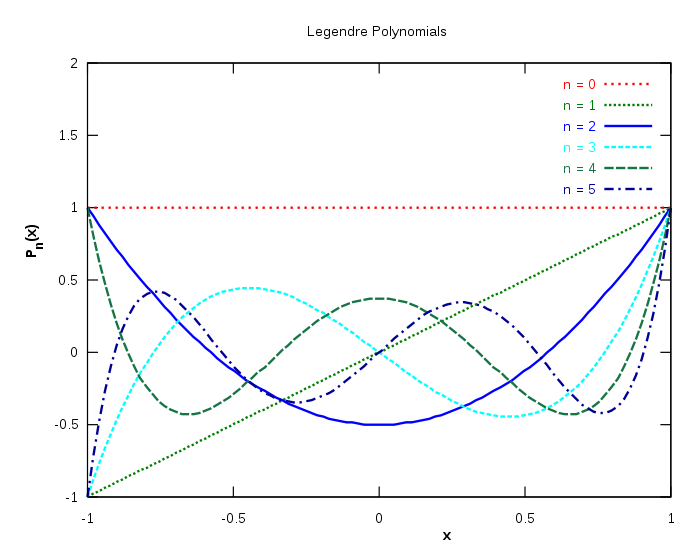
\includegraphics[scale=0.6]{figuras/legendre.png}
     \caption{Gráficos dos polinômios de Legendre com $n \le 5$}
 \end{figure}



 \textbf{Observação:} Vamos mostrar que $(p_n(t))_{n \ge 0}$ é base ortonormal para $L^2[-1,1].$ Tem-se
 \[
 p_n(t) = \frac{1}{2^n n!} \od[n]{}{t} (t^2 - 1)^n
 \]
 
 Segue do Teorema de Stone-Weierstrass que
 \[
 \mathcal{C}([-1,1], \mathbb{R}) = \overline{[t^n, n \ge 0 ]}^{\norm{\centerdot}_\infty} = \overline{[p_n , n \ge 0]}^{\norm{\centerdot}_\infty}
 \]
 Além disso,
 \[
 \norm{f}_2 \le \sqrt{2} \norm{f}_\infty \ \forall f \in L^2[-1,1] 
 \]
 Daí, $[p_n, n \ge 0]$ é denso em $(\mathcal{C}([-1,1], \mathbb{R}), \norm{\centerdot}_2),$ e $[p_n, n \ge 0]$ é denso em $L^2[-1,1].$
 
 Sendo que $(p_n)_{n \ge 0}$ é uma família ortonormal, segue do Teorema da Base Ortonormal que $(p_n)_{n \ge 0}$ é base ortonormal de $L^2[-1,1].$

}

\exercicio{16} Calcule o volume do paralelepípedo formado pelos vetores
\dividiritens{
\task[\pers{a}] $(1,-1,1,-1), (1,1,1,1),(1,0,-1,0),(0,1,0,-1).$
\task[\pers{b}] $(1,1,1,1),(1,-1,-1,1), (2,1,1,3),(0,1,-1,0).$
}

\solucao{}
\exercicio{17} No espaço euclidiano $\mathcal{P}_n(\mathbb{R})$ com o produto interno $\displaystyle\int\limits_{-1}^1 f(x)g(x) \dif x,$ calcule
\dividiritens{
\task[\pers{a}] o volume do paralelepípedo $P[1,x, \ldots, x^n];$
\task[\pers{b}] a distância do vetor $x^n$ até o subespaço $\mathcal{P}_{n-1}(\mathbb{R});$
\task[\pers{c}] o ângulo entre o vetor $x^n$ e o subespaço $\mathcal{P}_{n-1}(\mathbb{R});$
\task[\pers{d}] a distância do vetor $x^k$ até o subespaço $\mathcal{P}_{\ell}(\mathbb{R}),$ onde $k = 0, 1, \ldots, n$ e $\ell \le n;$
\task[\pers{e}] o ângulo entre o vetor $x^n$ e o subespaço $\mathcal{P}_{n-1}(\mathbb{R}),$ onde $k = 0, 1, \ldots, n$ e $\ell \le n.$
}
\solucao{
}


\exercicio{18} Considere $\mathcal{C}([0, 2 \pi], \mathbb{R})$ munido do produto interno
\[
\prin{f,g} = \displaystyle\int\limits_{0}^{2 \pi} f(x)g(x) \dif x.
\]
Determine a função $h \in \prin{1, \sen x, \cos x}$ que melhor se aproxime de $f \colon [0, 2 \pi] \to \mathbb{R} $ dada por $f(t) = t - 1.$
\solucao{}

\exercicio{19} Sabemos que é possível representar um sistema linear a partir de um operador linear $T \in \mathcal{L}(V,U)$, escrevendo o sistema na forma $Tx = b.$ Mesmo assim, esse sistema pode ser insolúvel. Vamos então procurar um $x$ tal que a distância para a imagem de $T$ seja a menor possível. Considere então $x \in U$ ta que para todo $v \in \mbox{Im }(T),$ tenhamos $\prin{T(x)-b,v} = 0.$
\dividiritens{
\task[\pers{a}] Prove que $x$ satisfaz
\[
(T^{*}T)(x) = T^{*}(b)
\]
\task[\pers{b}] Verifique que o sistema representado pela equação acima sempre possui solução.
}
\solucao{
\dividiritens{
\task[\pers{a}] Se $\prin{T(x)-b,v} = 0$ para todo $v \in \mbox{Im }(T),$ então $T(x)-b \in (\mbox{Im }(T))^{\perp}.$ Mas $(\mbox{Im }(T))^{\perp} = \Ker(T^{*}).$ Daí,
\[
T^{*}(T(x) - b) = 0 \Rightarrow (T^{*}T)(x) = T^{*}(b).
\]

\task[\pers{b}] Claramente $T(x) \in \mbox{Im }(T).$ Logo, o sistema $T^{*}(T(x)) = T^{*}(b)$ possui solução.
}
}

\exercicio{20} Determine a reta que melhor se ajusta aos pontos $(-1, -10), (0, -6), (1, -4), (2, -2)$ de $\mathbb{R}^2$.
\solucao{
Considere $\alpha x + \beta y + \gamma = 0$ a equação da reta desejada. Queremos que esses pontos pertençam à reta. Logo, formamos o seguinte sistema:
\[
\begin{cases}
-\alpha -10 \beta + \gamma = 0\\
-6 \beta + \gamma = 0\\
\alpha - 4 \beta + \gamma = 0\\
2\alpha - 2 \beta + \gamma = 0\\
\end{cases} \Rightarrow A = [T]_{\mbox{can}} = \begin{bmatrix}
-1 & -10 & 1 \\
0  & -6  & 1 \\
1  & -4  & 1 \\
2  & -2  & 1
\end{bmatrix} \begin{bmatrix}
\alpha \\ \beta \\ \gamma
\end{bmatrix} = \begin{bmatrix}
0 \\ 0 \\ 0
\end{bmatrix}
\]
Sendo $x = (\alpha, \beta, \gamma)^t$ e $b = (0,0,0)^t,$ queremos encontrar $x$ que resolva
\[
(A^{*}A)(x) = A^{*}(b).
\]
Logo, temos que
\[
\left(\begin{matrix}
6 & 2 & 2 \\
2 & 156 & -22 \\
2 & -22 & 4
\end{matrix}\right)   \begin{bmatrix}
\alpha \\ \beta \\ \gamma
\end{bmatrix} = \left(\begin{matrix}
-1 & 0 & 1 & 2 \\
-10 & -6 & -4 & -2 \\
1 & 1 & 1 & 1
\end{matrix}\right) \begin{bmatrix}
0 \\ 0 \\ 0
\end{bmatrix} \Rightarrow \begin{cases}
6\alpha + 2\beta + 2 \gamma =0 \\
2\alpha + 156\beta  -22 \gamma =0 \\
2\alpha  -22\beta + 4 \gamma =0
\end{cases}
\]
}

\exercicio{21} Determine o polinômio de grau $2$ que melhor se ajusta aos pontos $(-1, 0), (0, -1), (1, 1), (2, 4)$ de $\mathbb{R}^2$.
\solucao{}
\exercicio{22} Determine a melhor solução aproximada do sistema
\[
\begin{cases}
x-2y=1\\
x-y=0\\
2x+2y=2
\end{cases}
\]
\solucao{A matriz que representa o sistema será
\[
A = \begin{bmatrix}
1 & -2 \\
1 & -1 \\
2 & 2
\end{bmatrix}
\]
Logo, tomando $z = (x,y)^t$ e $b = (1,0,2)^t,$ 
\[
Az = b
\]
Vamos encontrar $z$ tal que $A^{*}Az = A^*b:$
\[
A^{*}Az = A^{*}b \Rightarrow \begin{bmatrix}
6 & 1 \\
1 & 9
\end{bmatrix}  \begin{bmatrix}
x \\
y
\end{bmatrix} = \begin{bmatrix}
1 & 1 & 2 \\
-2 & -1 & 2
\end{bmatrix}\begin{bmatrix}
1 \\
0 \\
2
\end{bmatrix} \Rightarrow \begin{cases}
6x+y = 5\\
x + 9y = 2
\end{cases} \Rightarrow Z = \left( \frac{43}{53}, \frac{7}{53} \right)
\]
Portanto, a melhor solução aproximada para o sistema será $\left( \frac{43}{53}, \frac{7}{53} \right).$
}


\exercicio{23} Considere o espaço vetorial $\mathcal{P}_3(\mathbb{R})$ com produto interno dado por
\[
\prin{f,g} = \displaystyle\int\limits_{0}^{1} f(x)g(x) \dif x.\]

Determine o polinômio do subespaço $\prin{1,x^2}$ que melhor se aproxima de $f(x) = x^3-x.$

\solucao{
Seja $W =\prin{1,x^2}.$ Vamos encontrar 
\[
d(f, W) = \{ \norm{f - w} | w \in W \} 
\]
Sabemos que $d(f,W) = \norm{f - E_W(f)},$ onde 
\[
E_W(f) = \sum\limits_{i=1}^2 \frac{\prin{f, w_i}}{\norm{w_i}^2} w_i =  \frac{\prin{f, 1}}{\norm{1}^2} + \frac{\prin{f, x^2}}{\norm{x^2}^2}
\]
Logo, 
\[
E(x^3 - x) = \frac{\prin{x^3 - x, 1}}{\norm{1}^2} + \frac{\prin{x^3 - x, x^2}}{\norm{x^2}^2} =  \frac{-\frac{1}{4}}{1} + \frac{-\frac{1}{12}}{\frac{1}{5}} = -\frac{2}{3}
\]
e
\[
d(f,W) = \norm{x^3 - x +\frac{2}{3}} = \displaystyle\int\limits_0^1  \left(x^3 - x +\frac{2}{3} \right) \left(x^3 - x +\frac{2}{3} \right)  \dif x = \frac{59}{315}.
\]
Basta encontrar um $g(x)$ tal que
\[
\norm{f - g} = \frac{59}{315}
\]

}


\exercicio{24}  Ache $a, b, c \in \mathbb{R}$ de forma a minimizar o valor da integral
\[
\displaystyle\int\limits_{-1}^1 \abs{x^3 - ax^2 - bx -c}^2 \dif x.
\]

\solucao{}

\exercicio{25}  Sejam $U, V$ espaços com produtos internos e $T \colon U \to V$ uma aplicação tal que $\prin{T(u), T(v)} = \prin{u, v} \ \forall u,v \in U.$ Mostre que $T$ é linear.

\solucao{Para verificar que $T$ é linear, precisamos mostrar que, para todo $u, v \in V$ e $\alpha \in K,$ temos que $T(u + v) =  T(u) + T(v)$ e $T(\alpha u) = \alpha T(u).$ De fato,
\begin{itemize}
    \item para $u,v, w\in U,$ temos que 
    \[\prin{T(u+v), T(w)} = \prin{(u+v),w} = \prin{u,w} + \prin{v,w} = \prin{T(u), T(w)} + \prin{T(v), T(w)} =\]\[ \prin{T(u) + T(v), T(w)} \Rightarrow T(u+v) = T(u) + T(v).\]
    \item para $u,v, w\in U,$ temos que 
    \[\prin{T(\alpha u), T(w)} = \prin{\alpha u,w} = \alpha \prin{u,w} = \alpha \prin{T(u), T(w)} + \prin{\alpha T(v), T(w)} \Rightarrow T(\alpha u) = \alpha T(u).\]

\end{itemize}
Logo, $T$ é linear.
}
\subsection*{Operadores lineares em espaços com produto interno}
\exercicio{26} Para cada um dos seguintes funcionais lineares $\varphi \in V^{*},$ encontre um vetor $u \in V$ tal que $\varphi(v) = \prin{v, u} \ \forall v \in V:$

\dividiritens{
\task[\pers{a}] $V = \mathbb{R}^3, \varphi(x,y,z) = x + 2y -3z;$
\task[\pers{b}] $V = \mathbb{C}^3, \varphi(x,y,z) = ix + (2+3i)y + (1-2i)z;$
\task[\pers{c}] $V = \mathcal{P}_2(\mathbb{R}), \varphi(f) = f(1);$
}

\solucao{\dividiritens{
\task[\pers{a}] Note que
\[
x +2y-3z = \prin{(1,2,-3),(x,y,z)}.
\]
Portanto, temos que para $u = (1,2,-3),$ $\varphi(v) = \prin{u, v}, \ \forall v \in V.$
\task[\pers{b}] Veja que
\[
 ix + (2+3i)y + (1-2i)z = \prin{(i,2+3i,1-2i),(x,y,z)}.
\]
Portanto, temos que para $u = (i,2+3i,1-2i),$ $\varphi(v) = \prin{u, v}, \ \forall v \in V.$

\task[\pers{c}] Sejam $f(x) = ax^2 + bx +c$ e $g(x) = \alpha x^2 + \beta x + \gamma.$ Como $f(1) = a + b + c,$ temos que
\[
\varphi(f) = a + b + c.
\]
Queremos encontrar $g$ tal que $\varphi(f) = \prin{g,f}.$ Logo, devemos ter
\[
\prin{g,f} = a + b + c \Rightarrow \prin{g,f} = \displaystyle\int\limits_{0}^1 g(x) f(x) \dif x \Rightarrow \displaystyle\int\limits_{0}^1 (\alpha x^2 + \beta x + \gamma) (ax^2 + bx +c) \dif x = a + b + x
\]
%https://www.wolframalpha.com/input/?i=%5Cint_0%5E1+%28%5Calpha+x%5E2+%2B+%5Cbeta+x+%2B+%5Cgamma%29+%28ax%5E2+%2B+bx+%2Bc%29++dx+%3D+a+%2B+b+%2B+c
}


}

\exercicio{27} Seja $V = \mathcal{P}_n(\mathbb{R}),$ com o produto interno usual
\[
\prin{f,g} = \displaystyle\int\limits_{0}^1 f(t) g(t) \dif t, \ \forall f,g \in V.
\]
Dado o funcional linear $\varphi \in V^{*},$ definido por
\[
\varphi(f) = f(\alpha), \alpha \in \mathbb{R},
\]
encontre $g \in V$ tal que $\varphi(f) = \prin{g,f}.$

\solucao{}

\exercicio{28} Seja $T \in \mathcal{L}(\mathbb{C}^2)$ o operador dado por $T(1, 0) = (7 + i, 8)$ e $T(0, 1) = (2i, i).$ Considerando $\mathbb{C}^2$ com o produto interno canônico, determine $T^{*}.$

\solucao{Observe que a representação matricial de $T$ na base canônica de $\mathbb{C}^2$ é
\[
A = [T]_{\mbox{can}} = \begin{bmatrix}
7 + i & 8 \\
2i & i
\end{bmatrix}
\]
Como a base canônica é uma base ortonormal, a matriz que representa $T^{*}$ na base canônica será a hermitiana de $A,$ ou seja,
\[
[T^{*}]_{\mbox{can}} = A^{H} = A^{*} = [T^{*}]_{\mbox{can}} = \overline{ \begin{bmatrix}
7 + i & 8 \\
2i & i
\end{bmatrix}^t} = \begin{bmatrix}
7 - i & -2i \\
8 & -i
\end{bmatrix}
\]
Logo, o operador $T^{*} \in \mathcal{L}(\mathbb{C}^2)$ é dado por $T^*(1,0) = (7-i,-2i)$ e $T^{*}(0,1) = (8,-i).$
}

\exercicio{29} Considere $\mathbb{C}^2$ com o produto interno canônico. Seja $T \in \mathcal{L}(\mathbb{C}^2)$ tal que sua matriz na base canônica é dada por
\[
a_{jk} = i^{j+k}, \ \mbox{onde i é a unidade imaginária.}
\]
Determine uma base de $\Ker T^{*}.$
\solucao{Como $T \in \mathcal{L}(\mathbb{C}^2),$ temos que $[T]_{\mbox{can}} \in \mathcal{M}_2(\mathbb{C}).$ Pela descrição do enunciado, trata-se da matriz
\[
A = [T]_{\mbox{can}} = \begin{bmatrix}
i^{1+1} & i^{1 + 2} \\
i^{2+1} & i^{2+2}
\end{bmatrix}  = \begin{bmatrix}
-1 & -i \\
-i & 1
\end{bmatrix}
\]
Como a base canônica é ortonormal, a matriz que representa $T^{*}$ na base canônica será exatamente a hermitiana da matriz que representa $T.$ Assim,
\[
 [T^{*}]_{\mbox{can}} = A^{H} = A^{*} = \overline{\begin{bmatrix}
-1 & -i \\
-i & 1
\end{bmatrix}^t } = \begin{bmatrix}
-1 & i \\
i & 1
\end{bmatrix}
\]
Considere agora $v = (x,y) \in \Ker(T^{*}).$ Devemos então ter
\[
A^{*}v = 0 \Rightarrow \begin{bmatrix}
-1 & i \\
i & 1
\end{bmatrix} \begin{bmatrix}
x \\ y
\end{bmatrix} = \begin{bmatrix}
0 \\ 0
\end{bmatrix} \Rightarrow \begin{cases}
-x+iy = 0\\
ix + y = 0
\end{cases} \Rightarrow v = y(i , 1)
\]
Portanto, $\{ (i,1) \}$ é uma base para $\Ker T^{*}.$
}

\exercicio{30} Sejam $V = \mathbb{C}^n$ com produto interno canônico e $v, w \in \mathbb{C}^n.$ Defina a aplicação
\[
\fullfunction{T}{\mathbb{C}^n}{\mathbb{C}^n}{u}{T(u) = \prin{u,v}w}
\]
\dividiritens{
\task[\pers{a}] Mostre que $T \in \mathcal{L}(\mathbb{C}^n).$
\task[\pers{b}] Descreva $T^{*}.$
\task[\pers{c}] Qual é a matriz de $T$ na base canônica de $\mathbb{C}^n?$ Qual é o posto dessa matriz?
}

\solucao{\dividiritens{
\task[\pers{a}] Vejamos que $T$ é linear:
\begin{itemize}
    \item $T(u_1 + u_2) = T(u_1) + T(u_2), \ \forall u_1, u_2 \in \mathbb{C}^n:$
    Temos que
    \[
    T(u_1 + u_2) = \prin{u_1 + u_2,v}w = (\prin{u_1,v} + \prin{u_2,v})w = \prin{u_1,v}w + \prin{u_2,v}w = T(u_1) + T(u_2).
    \]
   \item $T(\alpha u) = \alpha T(u), \ \forall u \in \mathbb{C}^n, \forall \alpha \in \mathbb{C}:$
    Temos que
    \[
    T(\alpha u) = \prin{\alpha u,v}w = \alpha \prin{u_,v}w = \alpha T(u).
    \]
\end{itemize}
Logo, $T \in \mathcal{L}(\mathbb{C}^n).$
\task[\pers{b}] Vamos encontrar a matriz que representa $T^{*}$ na base canônica de $\mathbb{C}^n.$ Lembramos que a base canônica é $\{e_1, e_2, \ldots, e_n \},$ onde
\[
e_i = (0, \ldots, 0, \underbrace{1}_{i-\mbox{ésima posição}},0, \ldots, 0).
\]
Vejamos como $T$ se comporta na base canônica. Dado $v = (v_1, v_2, \ldots, v_n) \in \mathbb{C}^n,$
\[
T(e_i) = \prin{e_i, v}w = v_iw
\]
Portanto, sendo $w = (w_1, w_2, \ldots, w_n),$ a matriz que representa $T$ na base canônica é
\[
A = [T]_{\mbox{can}} = \begin{bmatrix}
v_1w_1 & v_2w_1 & \ldots & v_nw_1 \\
v_1w_2 & v_2w_2 & \ldots & v_nw_2 \\
\vdots & \vdots & \ddots & \vdots \\
v_1w_n & v_2w_n & \ldots & v_nw_n \\
\end{bmatrix}.
\]
Como a base canônica é ortonormal, a matriz que representa $T^{*}$ na base canônica será a transposta conjugada de $A,$ ou seja, $A^H:$
\[
[T^{*}]_{\mbox{can}} = A^H = A^{*} = \overline{\begin{bmatrix}
v_1w_1 & v_2w_1 & \ldots & v_nw_1 \\
v_1w_2 & v_2w_2 & \ldots & v_nw_2 \\
\vdots & \vdots & \ddots & \vdots \\
v_1w_n & v_2w_n & \ldots & v_nw_n \\
\end{bmatrix}^t} = \begin{bmatrix}
\overline{v_1w_1} & \overline{v_1w_2} & \ldots & \overline{v_1w_n} \\
\overline{v_2w_1 }& \overline{v_2w_2} & \ldots & \overline{v_2w_n} \\
\vdots & \vdots & \ddots & \vdots \\
\overline{v_nw_1} & \overline{v_nw_2} & \ldots & \overline{v_nw_n} \\
\end{bmatrix}
\]
Assim, temos pela representação acima que
\[
T^{*}(e_i) = \overline{v w_i} = \overline{v} \prin{e_i, \overline{w}} \Rightarrow T^{*}(u) =  \overline{v} \prin{u, \overline{w}}.
\]
\task[\pers{c}] 
}
}
\exercicio{31} Encontre uma matriz ortogonal cuja primeira linha seja $\left( \frac{1}{3}, \frac{2}{3},\frac{2}{3}\right).$

\solucao{A matriz $P$ será ortogonal se os três vetores que compõem suas linhas forem ortonormais e ortogonais entre si. Ou seja, se $u_1, u_2, u_3$ formam as linhas da matriz, $\prin{u_1, u_2} = \prin{u_2,u_3} = \prin{u_1, u_3} = 0.$ Em nosso caso, $u_1 = \left( \frac{1}{3}, \frac{2}{3},\frac{2}{3}\right).$ Inicialmente, procuremos por um vetor não nulo $w_2 =(x, y, z)$ que seja ortogonal a $u_1,$ ou seja, para o qual
\[
0 = \prin{u_1, w_2} = \frac{x}{3} + \frac{2y}{3} + \frac{2z}{3} = 0.
\]
Uma solução para essa equação é $w_2 = (0,1,-1).$ Normalizando $w_2,$ poderemos encontrar a segunda linha para $P:$
\[
u_2 = \frac{w_2}{\norm{w_2}}= \frac{(0,1,-1)}{\sqrt{2}} = \left(0, \frac{\sqrt{2}}{2} ,- \frac{\sqrt{2}}{2} \right)
\]
Em seguida, devemos encontrar um vetor não nulo $w_3 = (x, y, z)$ que seja simultaneamente ortogonal a $u_1$ e a $u_2,$ ou seja, para o qual
\[
\begin{cases}
\prin{u_1,w} = 0 \\
\prin{u_2,w} = 0
\end{cases} \Rightarrow \begin{cases}
\frac{x}{3} + \frac{2y}{3} + \frac{2z}{3} = 0\\
\frac{y \sqrt{2}}{2} - \frac{z \sqrt{2}}{2} = 0
\end{cases} \Rightarrow \begin{cases}
x + 2y+2z = 0\\
y-z = 0
\end{cases}  \Rightarrow w_3 = z(-4,1,1)
\]
Logo, fazendo $z = 1,$ podemos tomar $w_3 = (-4,1,1).$ Daí, normalizando $w_3,$
\[
u_3 = \frac{w_3}{\norm{w_3}} = \frac{(-4,1,1)}{\sqrt{18}} = \left( -\frac{2\sqrt{2}}{3}, \frac{\sqrt{2}}{6}, \frac{\sqrt{2}}{6} \right)
\]
Dessa forma, obtemos a matriz
\[
P = \begin{bmatrix}
\frac{1}{3} & \frac{2}{3} & \frac{2}{3} \\
0 & \frac{\sqrt{2}}{2} & - \frac{\sqrt{2}}{2} \\
-\frac{2\sqrt{2}}{3} & \frac{\sqrt{2}}{6} & \frac{\sqrt{2}}{6}
\end{bmatrix}.
\]
É importante notar que a matriz $P$ não é única.
}
\exercicio{32} Prove que $\mbox{Im }T^{*} = (\Ker T)^{\perp}, \Ker T^{*} = (\mbox{Im }T)^{\perp}.$


\solucao{Veja itens a e b do exercício 15 da lista 5.}

\exercicio{33} Mostre que $T^*T = 0$ implica $T = 0.$

\solucao{Veja Exercício 21 da lista 5.}

\exercicio{34} Considere o produto interno
\[
\prin{f,g} = \displaystyle\int\limits_{-1}^1 f(x) g(x) \dif x.
\]
\dividiritens{
\task[\pers{a}] Tome $V = \mathcal{P}_n(\mathbb{R}),$ com o produto interno acima. Prove que o operador derivação $D$ não tem adjunto em $V.$ 

\task[\pers{b}] Seja $V$ o espaço de funções reais infinitamente deriváveis periódicos de período $1$ com o produto interno apresentado. Prove que o operador de derivação $D$ tem adjunto em $V$ e determine-o.
\task[\pers{c}] No espaço $V$ do item b, considere o operador definido por
\[
(T(f))(x) = \sen^2(2 \pi x) D^2(f) + 2 \pi \cos(4 \pi x) D(f).
\]
Prove que $T^{*} = T.$
}

\solucao{}

\exercicio{35} Seja $T$ um operador autoadjunto. Mostre que $\Ker T^2 = \Ker T.$

\solucao{Vamos mostrar as duas inclusões:
\begin{itemize}
    \item $\Ker T \subset \Ker T^2:$ é óbvio, bastando notar que, se $x \in \Ker T,$ então $T(x) = 0,$ e consequentemente \[T^2(x) = T(\textcolor{Red}{T(x)}) = T(\textcolor{Red}{0}) = 0.\]
    
    \item $\Ker T^2 \subset \Ker T:$ Sendo $T$ autoadjunto, então para todos $u, w \in V$ temos que
\[
\prin{T(u), w} = \prin{u, T(w)}
\]
Escrevendo $w = T(v),$ ficamos com
\[
\prin{T(u), \textcolor{Mahogany}{w}} = \prin{u, T(\textcolor{Mahogany}{w})} \Rightarrow \prin{T(u), \textcolor{Mahogany}{T(v)}} = \prin{u, T(\textcolor{Mahogany}{T(v)})} \Rightarrow \prin{T(u), T(v)} = \prin{u, T^2(v)}
\]
Seja $x \in \Ker T^2.$ Então, $T^2(x) = 0.$ Fazendo $u = v = x$ na expressão acima, vem
\[\prin{T(x), T(x)} = \prin{x, \textcolor{PineGreen}{T^2(x)}} = \prin{x, \textcolor{PineGreen}{0}} = 0 \Rightarrow \prin{T(x), T(x)} = 0 \Rightarrow \norm{T(x)}^2 = 0 \Rightarrow T(x) = 0.\]
Portanto, concluímos que $x \in \Ker T.$
\end{itemize}
Logo, $\Ker T^2 = \Ker T$ se $T$ for autoadjunto.
}

\exercicio{36} Seja $V$ um espaço complexo com produto interno. Prove que se $\prin{T(v), v}$ é real para
qualquer $v \in V,$ então $T$ é autoadjunto.

\solucao{Veja o exercício 18 da lista 5.}

\exercicio{37} Sejam $S$ e $T$ autoadjuntos. Mostre que $ST$ é autoadjunto se e somente se $ST = TS.$

\solucao{Veja o item a do exercício 23 da lista 5.}

\exercicio{38} Para cada uma das seguintes matrizes simétricas $A,$, encontre uma matriz ortogonal $P$ para a qual a matriz $P^tAP$ seja diagonal, ou seja, encontre a Forma Alternativa de cada matriz:

\dividiritensdiv{3}{
\task[\pers{a}] $A = \begin{pmatrix}
1 & 2 \\
2 & -2
\end{pmatrix}$
\task[\pers{b}] $B = \begin{pmatrix}
5 & 4 \\
4 & -1
\end{pmatrix}$
\task[\pers{c}] $C = \begin{pmatrix}
7 & 3 \\
3 & -1
\end{pmatrix}$
}
\solucao{
\dividiritens{
\task[\pers{a}] Vamos primeiramente encontrar os autovalores e autovetores de $A.$ Temos:
\[
p_A(\lambda) = \det(A - \lambda I) = \det \left( \begin{pmatrix}
1 & 2 \\
2 & -2
\end{pmatrix} - \begin{pmatrix}
\lambda & 0 \\
0 & \lambda
\end{pmatrix}  \right) = \det \left( \begin{pmatrix}
1-\lambda & 2 \\
2 & -2-\lambda
\end{pmatrix}  \right) = \lambda^2 + \lambda - 6
\]
Como $p_A(\lambda) = (\lambda + 3)(\lambda - 2),$ os autovalores são $\lambda_1 = -3$ e $\lambda_2 = 2.$ Encontremos autovetores associados a eles. Seja $v_i = (x_i,y_i)$ um autovetor associado a $\lambda_i, i =1,2.$ Então
\[
Av=  \lambda_1 v_1 \Rightarrow \begin{pmatrix}
1 & 2 \\
2 & -2
\end{pmatrix} \begin{pmatrix}
x_1 \\ y_1
\end{pmatrix} =  \begin{pmatrix}
-3x_1 \\ -3y_1
\end{pmatrix} \Rightarrow \begin{cases}
4x_1+2y_1 = 0 \\
2x_1 + y_1 = 0
\end{cases} \Rightarrow v_1 = y_1 \left(-\frac{1}{2}, 1 \right).
\]
Podemos tomar $v_1 = (-1,2)$ como autovetor associado a $\lambda_1 = -3.$ Analogamente,
\[
Av=  \lambda_2 v_2 \Rightarrow \begin{pmatrix}
1 & 2 \\
2 & -2
\end{pmatrix} \begin{pmatrix}
x_2 \\ y_2
\end{pmatrix} =  \begin{pmatrix}
2x_2 \\ 2y_2
\end{pmatrix} \Rightarrow \begin{cases}
-x_2+2y_2 = 0 \\
2x_2 - 4y_2 = 0
\end{cases} \Rightarrow v_2 = y_2 \left(2, 1 \right).
\]

Logo, temos que $v_2 = (2,1)$ é um autovetor associado a $\lambda_2 = 2.$ 
Podemos escolher as colunas da matriz $P$ como autovetores ortogonais normalizados de $A,$ e os elementos diagonais serão os autovalores associados.
Já que $A$ é simétrica, temos que$\prin{v_1, v_2} = 0.$ Basta agora normalizá-los. Dado que $\norm{v_1} = \norm{v_2} = \sqrt{5},$ os autovetores ortogonais normalizados de $A$ que procuramos são
\[
w_1 = \frac{v_1}{\norm{v_1}} = \frac{(-1,2)}{\sqrt{5}} = \left(-\frac{\sqrt{5}}{5}, \frac{2 \sqrt{5}}{5} \right) \quad \mbox{e} \quad w_2 = \frac{v_2}{\norm{v_2}} = \frac{(2,1)}{\sqrt{5}} = \left(\frac{2\sqrt{5}}{5}, \frac{ \sqrt{5}}{5} \right) 
\]
Portanto, temos que
\[
P = \begin{pmatrix}
-\frac{\sqrt{5}}{5} & \frac{2\sqrt{5}}{5} \\
\frac{2 \sqrt{5}}{5} & \frac{\sqrt{5}}{5} 
\end{pmatrix}
\]
De fato, uma rápida verificação confirma que
\[
 \begin{pmatrix}
-3 & 0 \\
0 & 2
\end{pmatrix} = \begin{pmatrix}
-\frac{\sqrt{5}}{5} & \frac{2\sqrt{5}}{5} \\
\frac{2 \sqrt{5}}{5} & \frac{\sqrt{5}}{5} 
\end{pmatrix}
 \begin{pmatrix}
1 & 2 \\
2 & -2
\end{pmatrix}
\begin{pmatrix}
-\frac{\sqrt{5}}{5} & \frac{2\sqrt{5}}{5} \\
\frac{2 \sqrt{5}}{5} & \frac{\sqrt{5}}{5} 
\end{pmatrix}
\]

\task[\pers{b}] Encontremos os autovalores e autovetores de $B:$
\[
p_B(\lambda) = \det(B - \lambda I) = \det \left( \begin{pmatrix}
5 & 4 \\
4 & -1
\end{pmatrix} - \begin{pmatrix}
\lambda & 0 \\
0 & \lambda
\end{pmatrix}  \right) = \det \left( \begin{pmatrix}
5-\lambda & 4 \\
4 & -1-\lambda
\end{pmatrix}  \right) = \lambda^2 - 4\lambda - 21
\]
Como $p_B(\lambda) = (\lambda + 3)(\lambda - 7),$ os autovalores são $\lambda_1 = -3$ e $\lambda_2 = 7.$ Encontremos autovetores associados a eles. Seja $v_i = (x_i,y_i)$ um autovetor associado a $\lambda_i, i =1,2.$ Então
\[
Bv=  \lambda_1 v_1 \Rightarrow \begin{pmatrix}
5 & 4 \\
4 & -1
\end{pmatrix} \begin{pmatrix}
x_1 \\ y_1
\end{pmatrix} =  \begin{pmatrix}
-3x_1 \\ -3y_1
\end{pmatrix} \Rightarrow \begin{cases}
8x_1+4y_1 = 0 \\
4x_1 + 2y_1 = 0
\end{cases} \Rightarrow v_1 = y_1 \left(-\frac{1}{2}, 1 \right).
\]
Podemos tomar $v_1 = (-1,2)$ como autovetor associado a $\lambda_1 = -3.$ Analogamente,
\[
Bv=  \lambda_2 v_2 \Rightarrow \begin{pmatrix}
5 & 4 \\
4 & -1
\end{pmatrix} \begin{pmatrix}
x_2 \\ y_2
\end{pmatrix} =  \begin{pmatrix}
7x_2 \\ 7y_2
\end{pmatrix} \Rightarrow \begin{cases}
-2x_2+4y_2 = 0 \\
4x_2 - 8y_2 = 0
\end{cases} \Rightarrow v_2 = y_2 \left(2, 1 \right).
\]

Logo, temos que $v_2 = (2,1)$ é um autovetor associado a $\lambda_2 = 7.$ 
Sendo $B$ simétrica, $\prin{v_1, v_2} = 0.$ Basta agora normalizá-los. Dado que $\norm{v_1} = \norm{v_2} = \sqrt{5},$ os autovetores ortogonais normalizados de $B$ que procuramos são
\[
w_1 = \frac{v_1}{\norm{v_1}} = \frac{(-1,2)}{\sqrt{5}} = \left(-\frac{\sqrt{5}}{5}, \frac{2 \sqrt{5}}{5} \right) \quad \mbox{e} \quad w_2 = \frac{v_2}{\norm{v_2}} = \frac{(2,1)}{\sqrt{5}} = \left(\frac{2\sqrt{5}}{5}, \frac{ \sqrt{5}}{5} \right) 
\]
Portanto, temos que
\[
P = \begin{pmatrix}
-\frac{\sqrt{5}}{5} & \frac{2\sqrt{5}}{5} \\
\frac{2 \sqrt{5}}{5} & \frac{\sqrt{5}}{5} 
\end{pmatrix}
\]
Assim,
\[
 \begin{pmatrix}
-3 & 0 \\
0 & 7
\end{pmatrix} = \begin{pmatrix}
-\frac{\sqrt{5}}{5} & \frac{2\sqrt{5}}{5} \\
\frac{2 \sqrt{5}}{5} & \frac{\sqrt{5}}{5} 
\end{pmatrix}
 \begin{pmatrix}
5 & 4 \\
4 & -1
\end{pmatrix}
\begin{pmatrix}
-\frac{\sqrt{5}}{5} & \frac{2\sqrt{5}}{5} \\
\frac{2 \sqrt{5}}{5} & \frac{\sqrt{5}}{5} 
\end{pmatrix}
\]

\task[\pers{c}] Encontremos os autovalores e autovetores de $C:$
\[
p_C(\lambda) = \det(C - \lambda I) = \det \left( \begin{pmatrix}
7 & 3 \\
3 & -1
\end{pmatrix} - \begin{pmatrix}
\lambda & 0 \\
0 & \lambda
\end{pmatrix}  \right) = \det \left( \begin{pmatrix}
7-\lambda & 3 \\
3 & -1-\lambda
\end{pmatrix}  \right) = \lambda^2 - 6\lambda - 16
\]
Como $p_B(\lambda) = (\lambda + 2)(\lambda - 8),$ os autovalores são $\lambda_1 = -2$ e $\lambda_2 = 8.$ Encontremos autovetores associados a eles. Seja $v_i = (x_i,y_i)$ um autovetor associado a $\lambda_i, i =1,2.$ Então
\[
Cv=  \lambda_1 v_1 \Rightarrow \begin{pmatrix}
7 & 3 \\
3 & -1
\end{pmatrix} \begin{pmatrix}
x_1 \\ y_1
\end{pmatrix} =  \begin{pmatrix}
-2x_1 \\ -2y_1
\end{pmatrix} \Rightarrow \begin{cases}
9x_1+3y_1 = 0 \\
3x_1 + y_1 = 0
\end{cases} \Rightarrow v_1 = y_1 \left(-\frac{1}{3}, 1 \right).
\]
Podemos tomar $v_1 = (-1,3)$ como autovetor associado a $\lambda_1 = -2.$ Analogamente,
\[
Cv=  \lambda_2 v_2 \Rightarrow \begin{pmatrix}
7 & 3 \\
3 & -1
\end{pmatrix} \begin{pmatrix}
x_2 \\ y_2
\end{pmatrix} =  \begin{pmatrix}
8x_2 \\ 8y_2
\end{pmatrix} \Rightarrow \begin{cases}
-x_2+3y_2 = 0 \\
3x_2 - 9y_2 = 0
\end{cases} \Rightarrow v_2 = y_2 \left(3, 1 \right).
\]

Logo, temos que $v_2 = (3,1)$ é um autovetor associado a $\lambda_2 = 8.$ 
Sendo $B$ simétrica, $\prin{v_1, v_2} = 0.$ Basta agora normalizá-los. Dado que $\norm{v_1} = \norm{v_2} = \sqrt{10},$ os autovetores ortogonais normalizados de $B$ que procuramos são
\[
w_1 = \frac{v_1}{\norm{v_1}} = \frac{(-1,3)}{\sqrt{10}} = \left(-\frac{\sqrt{10}}{10}, \frac{3 \sqrt{10}}{10} \right) \quad \mbox{e} \quad w_2 = \frac{v_2}{\norm{v_2}} = \frac{(3,1)}{\sqrt{10}} = \left(\frac{3\sqrt{10}}{10}, \frac{ \sqrt{10}}{10} \right) 
\]
Portanto, 
\[
P = \begin{pmatrix}
-\frac{\sqrt{10}}{10} & \frac{3\sqrt{10}}{10} \\
\frac{3 \sqrt{10}}{10} & \frac{\sqrt{10}}{10} 
\end{pmatrix}
\]
Logo,
\[
 \begin{pmatrix}
-2 & 0 \\
0 & 8
\end{pmatrix} = \begin{pmatrix}
-\frac{\sqrt{10}}{10} & \frac{3\sqrt{10}}{10} \\
\frac{3 \sqrt{10}}{10} & \frac{\sqrt{10}}{10} 
\end{pmatrix}
 \begin{pmatrix}
7 & 3 \\
3 & -1
\end{pmatrix}
\begin{pmatrix}
-\frac{\sqrt{10}}{10} & \frac{3\sqrt{10}}{10} \\
\frac{3 \sqrt{10}}{10} & \frac{\sqrt{10}}{10}  
\end{pmatrix}
\]
} 
}

\exercicio{39} Seja $T \in \mathcal{L}(\mathbb{C}^2)$ definido por $T(1, 0) = (1 + i, 2)$ e $T(0, 1) = (i, i).$ $T$ é normal?

\solucao{Não. Veja o exercício 14 da lista 5.}

\exercicio{40} Sejam $V$ um espaço unitário e $T \in \mathcal{L}(V)$ um operador normal. Mostre que
\dividiritens{
\task[\pers{a}] $T$ é autoadjunto se e somente se $\mbox{Spec }T \subseteq \mathbb{R}.$
\task[\pers{b}] $T$ é unitário se e somente se, para todo $\lambda \in \mbox{Spec }T, \abs{\lambda} = 1.$
}

\solucao{
\dividiritens{
\task[\pers{a}] Seja $\lambda$ um autovalor de $T.$ Considere $v \neq 0$ um autovetor associado a $\lambda,$ ou seja, tal que $T(v) = \lambda v.$ Observe que
\[
\begin{array}{rcl}
\lambda \prin{v,v} &=& \prin{\textcolor{Cerulean}{\lambda v},v } \\
&=& \prin{\textcolor{Cerulean}{T(v)},v } \\
&=& \prin{v, \textcolor{Blue}{T^{*}}(v)} \\
&=& \prin{v, \textcolor{Blue}{T}(v)} \\
&=& \overline{\prin{\textcolor{Cerulean}{T(v)},v}} \\
&=& \overline{\prin{\textcolor{Cerulean}{\lambda v},v}} \\
&=& \overline{\lambda} \prin{v,v}
\end{array}
\]
Como $v \neq 0,$ então $\prin{v,v} \neq 0.$ Portanto,
\[
\lambda \prin{v,v} = \overline{\lambda} \prin{v,v} \Rightarrow \lambda = \overline{\lambda} \Rightarrow \lambda \in \mathbb{R}.
\]
A recíproca é análoga.
\task[\pers{b}] Sabemos que um operador unitário preserva o produto interno, isto é, para todos $u, v \in V,$
\[
\prin{T(u), T(v) } = \prin{u,v}
\]
tome $\lambda$ um autovalor de $T$ e  $w \neq 0$ um autovetor associado a $\lambda.$ Então, $T(w) = \lambda w,$ e daí
\[
\prin{w,w} = \prin{T(w), T(w) } = \prin{\lambda w, \lambda w} = \lambda \overline{\lambda} \prin{w,w} = \abs{\lambda}^2 \prin{w,w}
\]
Sendo $\prin{w,w} \neq 0,$ pois $w$ é um autovetor, então concluímos que $\abs{\lambda}^2 = 1 \Rightarrow \abs{\lambda} = 1.$
Novamente, a recíproca é análoga.
}
}

\exercicio{41} Seja $V = \mathbb{R}^n$ com produto interno usual e $T \in \mathcal{L}(\mathbb{R}^n).$ Suponhamos que $v_1 = (1, 1, \ldots , 1), v_2 = (1, 1, \ldots , 1, 0), \ldots , v_n = (1, 0, .\ldots, 0)$ sejam autovetores de $T.$
Mostre que $T$ é autoadjunto se e somente se $T$ possui um único autovalor.
\solucao{$(\Rightarrow)$ Suponha que $T$ seja autoadjunto. Considere $\lambda_i \in \mathbb{R}$ (pelo exercício 40) autovalores distintos de $T.$ Temos portanto que:
\[
T(1, 1, \ldots , 1) = \lambda_1(1, 1, \ldots , 1)
\]


}

\exercicio{42} Consideremos $V = \mathbb{C}$ como um $\mathbb{R}$-espaço vetorial.
\dividiritens{
\task[\pers{a}] Mostre que $\prin{\alpha, \beta} = \mbox{Re}(\alpha \overline{\beta})$ é um produto interno em $\mathbb{C}.$

\task[\pers{b}] Para cada $\gamma \in V,$ seja a função $M_{\gamma} \colon \mathbb{C} \to \mathbb{C}$ dada por $M_{\gamma}(\alpha) = \gamma \alpha.$ Mostrar
que $(M_{\gamma})^{*} = M_{\overline{\gamma}}.$

\task[\pers{c}] Para quais $\gamma \in \mathbb{C}$, $M_{\gamma}$ é autoadjunto?

\task[\pers{d}] Para quais $\gamma \in \mathbb{C}$, $M_{\gamma}$ é unitário?
}

\solucao{
\dividiritens{
\task[\pers{a}] Vaamos verificar os axiomas de produto interno:
\begin{itemize}
    \item[$\clubsuit$] $\prin{\alpha+\beta, \gamma} = \prin{\alpha, \gamma} + \prin{\beta, \gamma}.$
    Sejam $\alpha = \alpha_1 + i \alpha_2, \beta = \beta_1 + \beta_2 i, \gamma = \gamma_1 + \gamma_2 i \in \mathbb{C}.$ Então
    \[
    \prin{\alpha+\beta, \gamma} =  \mbox{Re}((\alpha+\beta) \overline{\gamma}) =  \mbox{Re}((\alpha_1 + i \alpha_2+\beta_1 + \beta_2 i) \overline{ \gamma_1 + \gamma_2 i}) =  \mbox{Re}(((\alpha_1 + \beta_1) + i (\alpha_2+\beta_2))(\gamma_1 - \gamma_2 i))
    \]
    \item[$\textcolor{Red}{\varheart}$]
    \item[$\spadesuit$]
    \item[$\textcolor{Red}{\vardiamond}$]
\end{itemize}
}

}

\textcolor{white}{oi}
\newline
\textcolor{Red}{Questões Suplementares}


\exercicio{k} Prove que para qualquer triângulo, a soma dos quadrados das medidas de suas três medianas é igual a três quartos da soma dos quadrados das medidas de seus lados.

%https://repositorio.unesp.br/bitstream/handle/11449/144302/pontes_rc_me_rcla.pdf?sequence=3


\solucao{}

\exercicio{k+1} Considere um tetraedro. Chamamos de \emph{bimediana} o segmento que liga os pontos médios de duas
arestas opostas do tetraedro.
\dividiritens{
\task[\pers{a}] Prove que, para qualquer tetraedro, a soma dos quadrados das medidas de suas três bimedianas é igual a um quarto da soma dos quadrados das medidas de suas arestas.

\task[\pers{b}] Encontre  %https://repositorio.unesp.br/bitstream/handle/11449/144302/pontes_rc_me_rcla.pdf?sequence=3
}
\solucao{}

\exercicio{k+2} Lembramos que, dado $T \in \mathcal{L}(V),$ definimos o \emph{espectro} de $T$ por
\[
\mbox{Spec }(T) = \{\lambda \in K| \lambda \mbox{ é autovalor de T.} \}
\]
Suponha que $T$ seja um operador normal.
\dividiritens{
\task[\pers{a}] Prove que $\overline{\mbox{Spec }(T)} \subseteq \mbox{Spec }(T^{*}).$
\task[\pers{b}] Seja $T \colon \mathbb{C}^2 \to \mathbb{C}^2$ dado por $T(1,0) = (1,1)$ e $T(0,1) = (1, 3+2i).$ Encontre os autovalores de $T^{*}.$
}
\newpage
\section{\textcolor{Floresta}{Lista 6}}

   \exercicio{1}
   
   
   \textcolor{Red}{Questões Suplementares}

\exercicio{31} 
\solucao{}
\end{document} 

%Interessante:

%https://en.wikipedia.org/wiki/Berlekamp%E2%80%93Massey_algorithm
%https://math.stackexchange.com/questions/1186477/given-minimal-characteristic-polynomial-how-to-derive-linear-recurrence

%http://www.kurims.kyoto-u.ac.jp/~kyodo/kokyuroku/contents/pdf/2033-19.pdf

%http://correio.fdvmg.edu.br/downloads/DET142/alglin_UFF.pdf